% Generated by Sphinx.
\def\sphinxdocclass{puthesis}
\documentclass[a4paper,10pt,english,lof,lot,twoside]{puthesis}
\usepackage[utf8]{inputenc}
\DeclareUnicodeCharacter{00A0}{\nobreakspace}
\usepackage{cmap}

\usepackage{babel}


\usepackage{longtable}

\usepackage{multirow}

\setcounter{tocdepth}{1}
\input{preamble._tex}
\usepackage{sphinx}


\title{AlphaTrainer - an Android based neurofeedback system using low-cost consumer Brain-Computer Interfaces}
\date{December 01, 2013}
\release{0.1}
\author{Martin Poulsen and Pelle Krøgholt}
\newcommand{\sphinxlogo}{}
\renewcommand{\releasename}{Release}
\makeindex

\makeatletter
\def\PYG@reset{\let\PYG@it=\relax \let\PYG@bf=\relax%
    \let\PYG@ul=\relax \let\PYG@tc=\relax%
    \let\PYG@bc=\relax \let\PYG@ff=\relax}
\def\PYG@tok#1{\csname PYG@tok@#1\endcsname}
\def\PYG@toks#1+{\ifx\relax#1\empty\else%
    \PYG@tok{#1}\expandafter\PYG@toks\fi}
\def\PYG@do#1{\PYG@bc{\PYG@tc{\PYG@ul{%
    \PYG@it{\PYG@bf{\PYG@ff{#1}}}}}}}
\def\PYG#1#2{\PYG@reset\PYG@toks#1+\relax+\PYG@do{#2}}

\expandafter\def\csname PYG@tok@gd\endcsname{\def\PYG@tc##1{\textcolor[rgb]{0.63,0.00,0.00}{##1}}}
\expandafter\def\csname PYG@tok@gu\endcsname{\let\PYG@bf=\textbf\def\PYG@tc##1{\textcolor[rgb]{0.50,0.00,0.50}{##1}}}
\expandafter\def\csname PYG@tok@gt\endcsname{\def\PYG@tc##1{\textcolor[rgb]{0.00,0.27,0.87}{##1}}}
\expandafter\def\csname PYG@tok@gs\endcsname{\let\PYG@bf=\textbf}
\expandafter\def\csname PYG@tok@gr\endcsname{\def\PYG@tc##1{\textcolor[rgb]{1.00,0.00,0.00}{##1}}}
\expandafter\def\csname PYG@tok@cm\endcsname{\let\PYG@it=\textit\def\PYG@tc##1{\textcolor[rgb]{0.25,0.50,0.56}{##1}}}
\expandafter\def\csname PYG@tok@vg\endcsname{\def\PYG@tc##1{\textcolor[rgb]{0.73,0.38,0.84}{##1}}}
\expandafter\def\csname PYG@tok@m\endcsname{\def\PYG@tc##1{\textcolor[rgb]{0.13,0.50,0.31}{##1}}}
\expandafter\def\csname PYG@tok@mh\endcsname{\def\PYG@tc##1{\textcolor[rgb]{0.13,0.50,0.31}{##1}}}
\expandafter\def\csname PYG@tok@cs\endcsname{\def\PYG@tc##1{\textcolor[rgb]{0.25,0.50,0.56}{##1}}\def\PYG@bc##1{\setlength{\fboxsep}{0pt}\colorbox[rgb]{1.00,0.94,0.94}{\strut ##1}}}
\expandafter\def\csname PYG@tok@ge\endcsname{\let\PYG@it=\textit}
\expandafter\def\csname PYG@tok@vc\endcsname{\def\PYG@tc##1{\textcolor[rgb]{0.73,0.38,0.84}{##1}}}
\expandafter\def\csname PYG@tok@il\endcsname{\def\PYG@tc##1{\textcolor[rgb]{0.13,0.50,0.31}{##1}}}
\expandafter\def\csname PYG@tok@go\endcsname{\def\PYG@tc##1{\textcolor[rgb]{0.20,0.20,0.20}{##1}}}
\expandafter\def\csname PYG@tok@cp\endcsname{\def\PYG@tc##1{\textcolor[rgb]{0.00,0.44,0.13}{##1}}}
\expandafter\def\csname PYG@tok@gi\endcsname{\def\PYG@tc##1{\textcolor[rgb]{0.00,0.63,0.00}{##1}}}
\expandafter\def\csname PYG@tok@gh\endcsname{\let\PYG@bf=\textbf\def\PYG@tc##1{\textcolor[rgb]{0.00,0.00,0.50}{##1}}}
\expandafter\def\csname PYG@tok@ni\endcsname{\let\PYG@bf=\textbf\def\PYG@tc##1{\textcolor[rgb]{0.84,0.33,0.22}{##1}}}
\expandafter\def\csname PYG@tok@nl\endcsname{\let\PYG@bf=\textbf\def\PYG@tc##1{\textcolor[rgb]{0.00,0.13,0.44}{##1}}}
\expandafter\def\csname PYG@tok@nn\endcsname{\let\PYG@bf=\textbf\def\PYG@tc##1{\textcolor[rgb]{0.05,0.52,0.71}{##1}}}
\expandafter\def\csname PYG@tok@no\endcsname{\def\PYG@tc##1{\textcolor[rgb]{0.38,0.68,0.84}{##1}}}
\expandafter\def\csname PYG@tok@na\endcsname{\def\PYG@tc##1{\textcolor[rgb]{0.25,0.44,0.63}{##1}}}
\expandafter\def\csname PYG@tok@nb\endcsname{\def\PYG@tc##1{\textcolor[rgb]{0.00,0.44,0.13}{##1}}}
\expandafter\def\csname PYG@tok@nc\endcsname{\let\PYG@bf=\textbf\def\PYG@tc##1{\textcolor[rgb]{0.05,0.52,0.71}{##1}}}
\expandafter\def\csname PYG@tok@nd\endcsname{\let\PYG@bf=\textbf\def\PYG@tc##1{\textcolor[rgb]{0.33,0.33,0.33}{##1}}}
\expandafter\def\csname PYG@tok@ne\endcsname{\def\PYG@tc##1{\textcolor[rgb]{0.00,0.44,0.13}{##1}}}
\expandafter\def\csname PYG@tok@nf\endcsname{\def\PYG@tc##1{\textcolor[rgb]{0.02,0.16,0.49}{##1}}}
\expandafter\def\csname PYG@tok@si\endcsname{\let\PYG@it=\textit\def\PYG@tc##1{\textcolor[rgb]{0.44,0.63,0.82}{##1}}}
\expandafter\def\csname PYG@tok@s2\endcsname{\def\PYG@tc##1{\textcolor[rgb]{0.25,0.44,0.63}{##1}}}
\expandafter\def\csname PYG@tok@vi\endcsname{\def\PYG@tc##1{\textcolor[rgb]{0.73,0.38,0.84}{##1}}}
\expandafter\def\csname PYG@tok@nt\endcsname{\let\PYG@bf=\textbf\def\PYG@tc##1{\textcolor[rgb]{0.02,0.16,0.45}{##1}}}
\expandafter\def\csname PYG@tok@nv\endcsname{\def\PYG@tc##1{\textcolor[rgb]{0.73,0.38,0.84}{##1}}}
\expandafter\def\csname PYG@tok@s1\endcsname{\def\PYG@tc##1{\textcolor[rgb]{0.25,0.44,0.63}{##1}}}
\expandafter\def\csname PYG@tok@gp\endcsname{\let\PYG@bf=\textbf\def\PYG@tc##1{\textcolor[rgb]{0.78,0.36,0.04}{##1}}}
\expandafter\def\csname PYG@tok@sh\endcsname{\def\PYG@tc##1{\textcolor[rgb]{0.25,0.44,0.63}{##1}}}
\expandafter\def\csname PYG@tok@ow\endcsname{\let\PYG@bf=\textbf\def\PYG@tc##1{\textcolor[rgb]{0.00,0.44,0.13}{##1}}}
\expandafter\def\csname PYG@tok@sx\endcsname{\def\PYG@tc##1{\textcolor[rgb]{0.78,0.36,0.04}{##1}}}
\expandafter\def\csname PYG@tok@bp\endcsname{\def\PYG@tc##1{\textcolor[rgb]{0.00,0.44,0.13}{##1}}}
\expandafter\def\csname PYG@tok@c1\endcsname{\let\PYG@it=\textit\def\PYG@tc##1{\textcolor[rgb]{0.25,0.50,0.56}{##1}}}
\expandafter\def\csname PYG@tok@kc\endcsname{\let\PYG@bf=\textbf\def\PYG@tc##1{\textcolor[rgb]{0.00,0.44,0.13}{##1}}}
\expandafter\def\csname PYG@tok@c\endcsname{\let\PYG@it=\textit\def\PYG@tc##1{\textcolor[rgb]{0.25,0.50,0.56}{##1}}}
\expandafter\def\csname PYG@tok@mf\endcsname{\def\PYG@tc##1{\textcolor[rgb]{0.13,0.50,0.31}{##1}}}
\expandafter\def\csname PYG@tok@err\endcsname{\def\PYG@bc##1{\setlength{\fboxsep}{0pt}\fcolorbox[rgb]{1.00,0.00,0.00}{1,1,1}{\strut ##1}}}
\expandafter\def\csname PYG@tok@kd\endcsname{\let\PYG@bf=\textbf\def\PYG@tc##1{\textcolor[rgb]{0.00,0.44,0.13}{##1}}}
\expandafter\def\csname PYG@tok@ss\endcsname{\def\PYG@tc##1{\textcolor[rgb]{0.32,0.47,0.09}{##1}}}
\expandafter\def\csname PYG@tok@sr\endcsname{\def\PYG@tc##1{\textcolor[rgb]{0.14,0.33,0.53}{##1}}}
\expandafter\def\csname PYG@tok@mo\endcsname{\def\PYG@tc##1{\textcolor[rgb]{0.13,0.50,0.31}{##1}}}
\expandafter\def\csname PYG@tok@mi\endcsname{\def\PYG@tc##1{\textcolor[rgb]{0.13,0.50,0.31}{##1}}}
\expandafter\def\csname PYG@tok@kn\endcsname{\let\PYG@bf=\textbf\def\PYG@tc##1{\textcolor[rgb]{0.00,0.44,0.13}{##1}}}
\expandafter\def\csname PYG@tok@o\endcsname{\def\PYG@tc##1{\textcolor[rgb]{0.40,0.40,0.40}{##1}}}
\expandafter\def\csname PYG@tok@kr\endcsname{\let\PYG@bf=\textbf\def\PYG@tc##1{\textcolor[rgb]{0.00,0.44,0.13}{##1}}}
\expandafter\def\csname PYG@tok@s\endcsname{\def\PYG@tc##1{\textcolor[rgb]{0.25,0.44,0.63}{##1}}}
\expandafter\def\csname PYG@tok@kp\endcsname{\def\PYG@tc##1{\textcolor[rgb]{0.00,0.44,0.13}{##1}}}
\expandafter\def\csname PYG@tok@w\endcsname{\def\PYG@tc##1{\textcolor[rgb]{0.73,0.73,0.73}{##1}}}
\expandafter\def\csname PYG@tok@kt\endcsname{\def\PYG@tc##1{\textcolor[rgb]{0.56,0.13,0.00}{##1}}}
\expandafter\def\csname PYG@tok@sc\endcsname{\def\PYG@tc##1{\textcolor[rgb]{0.25,0.44,0.63}{##1}}}
\expandafter\def\csname PYG@tok@sb\endcsname{\def\PYG@tc##1{\textcolor[rgb]{0.25,0.44,0.63}{##1}}}
\expandafter\def\csname PYG@tok@k\endcsname{\let\PYG@bf=\textbf\def\PYG@tc##1{\textcolor[rgb]{0.00,0.44,0.13}{##1}}}
\expandafter\def\csname PYG@tok@se\endcsname{\let\PYG@bf=\textbf\def\PYG@tc##1{\textcolor[rgb]{0.25,0.44,0.63}{##1}}}
\expandafter\def\csname PYG@tok@sd\endcsname{\let\PYG@it=\textit\def\PYG@tc##1{\textcolor[rgb]{0.25,0.44,0.63}{##1}}}

\def\PYGZbs{\char`\\}
\def\PYGZus{\char`\_}
\def\PYGZob{\char`\{}
\def\PYGZcb{\char`\}}
\def\PYGZca{\char`\^}
\def\PYGZam{\char`\&}
\def\PYGZlt{\char`\<}
\def\PYGZgt{\char`\>}
\def\PYGZsh{\char`\#}
\def\PYGZpc{\char`\%}
\def\PYGZdl{\char`\$}
\def\PYGZhy{\char`\-}
\def\PYGZsq{\char`\'}
\def\PYGZdq{\char`\"}
\def\PYGZti{\char`\~}
% for compatibility with earlier versions
\def\PYGZat{@}
\def\PYGZlb{[}
\def\PYGZrb{]}
\makeatother

\begin{document}

\makefrontmatter

\phantomsection\label{index_tex::doc}



\chapter{Introduction}
\label{ch-intro/index:introduction}\label{ch-intro/index:ch-intro}\label{ch-intro/index::doc}

\section{Neurofeedback, stress and brain-computer interfaces}
\label{ch-intro/index:ch-intro-neurofeedback-stress-and-bci}\label{ch-intro/index:neurofeedback-stress-and-brain-computer-interfaces}
Neurofeedback training (or neurofeedback therapy) is based on giving real time
feedback on brain activity. This feedback enables the brain to navigate towards
some desired brain state. Certain brain states have been shown to be
positively correlated with cognitive performance, de-stressing etc. Such brain
states form the goal for the neurofeedback.

Stress - a big and growing problem to both society and individuals -
is one of the conditions neurofeedback therapy is targeting within a
clinical context. For example, it is used within the US army as treatment
for veteran soldiers suffering from post-traumatic stress disorder
(PTSD) \cite{white_alphatheta_2009}. However,
neurofeedback systems targeting consumers remain rare and expensive
due to the required specialized hardware - in order to sense brain
states, a neurofeedback system includes a Brain-Computer Interface
(BCI). Though most BCIs are expensive and aimed at professionals,
within recent years a number of BCIs targeting consumers with prices
starting from \$ 50,- have emerged. Interaxon's \emph{Muse} \footnote{
\href{http://www.interaxon.ca}{http://www.interaxon.ca}
} BCI exemplifies the new generation of
discrete consumer BCIs (Figure \ref{ch-intro/index:fig-muse-headband}).
\begin{figure}[tbp]
\centering
\capstart

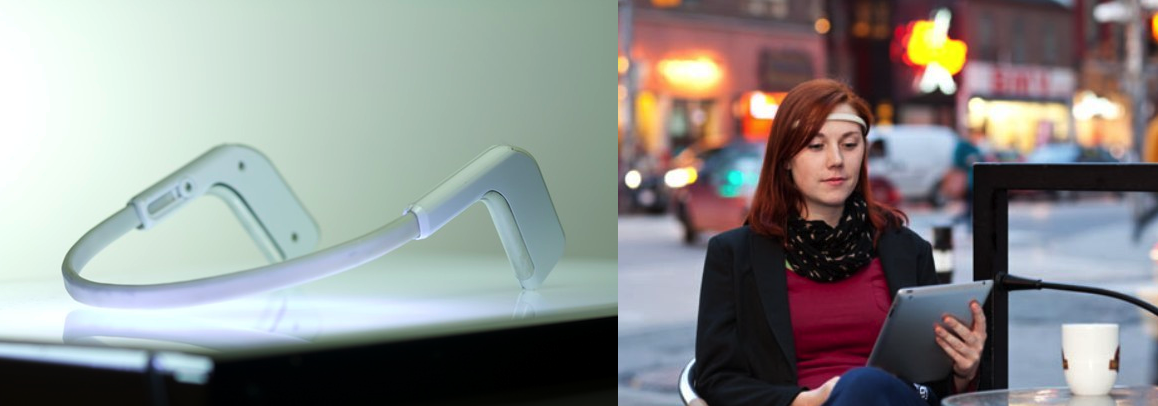
\includegraphics[width=0.800\linewidth]{muse-headband-collage.png}
\caption[Muse consumer BCI]{Muse consumer BCI (Image courtesy of Interaxon).}\label{ch-intro/index:fig-muse-headband}\end{figure}

The combination of the emerging consumer interfaces and the prospects of
neurofeedback motivates our hypothesis.


\section{Hypothesis}
\label{ch-intro/index:ch-intro-hypothesis-goals}\label{ch-intro/index:hypothesis}
We hypothesize that it is feasible to build a neurofeedback system comprising of
a consumer BCI and a mobile device which will enable neurofeedback training in
an everyday setting.

To test our hypothesis, we have set the following goals:

G1
\begin{quote}

Evaluate relevant consumer BCI's feasibility for neurofeedback training.
\end{quote}

G2
\begin{quote}

Design, implement and evaluate AlphaTrainer - a system enabling
neurofeedback training in an everyday setting.
\end{quote}

If such a system shows feasible, it would enable wide adoption of
neurofeedback training in eliminating the obstacle of expensive hardware. This
could move the neurofeedback practice out of a clinical setting and into the
homes and workplaces of people motivated to reduce their stress.


\section{Method}
\label{ch-intro/index:ch-intro-method}\label{ch-intro/index:method}
The vision and goal of AlphaTrainer - to enable neurofeedback training in an everyday
context - is rooted in the ideas of the early pioneers of ubiquitous computing
(ubicomp) who envisioned invisible computing, prototypes and the move away
from desktop computers into devices that ``\emph{weave themselves into the fabric of
everyday life}`` \cite{weiser_computer_1991} \cite{weiser_world_1994} \cite{weiser_computer_1999}.

In short, our method is to design, implement, deploy and evaluate
AlphaTrainer. This approach is inspired by later adapters of ubicomp stressing
the importance of deploying working systems for real usage. For example, Bardram
and Friday argue that ``\emph{...  the most valuable lessons to take from looking at
successful ubicomp systems is the need to mature the system through actual use}`` \cite{bardram_ubiquitous_2010}. By deploying AlphaTrainer for actual
use in an everyday context, we are able to learn about the system and
the usage ``\emph{in situ}'' which can not be investigated in a lab or by means of
lo-fi prototypes.

The process of building AlphaTrainer involves several activities. Which can be
mapped and understood through a framework proposed by Mackay and Fayard \cite{mackay_hci_1997}. The framework explains how HCI research can benefit
from triangulating across science and design disciplines while continuously
producing artifacts. Figure \ref{ch-intro/index:fig-triangulation} outlines the major
activities of this thesis. The arrows between activities show when output of
one activity has been fed into another thus mapping how activities have
benefited from each other across disciplines.
\begin{figure}[tbp]
\centering
\capstart

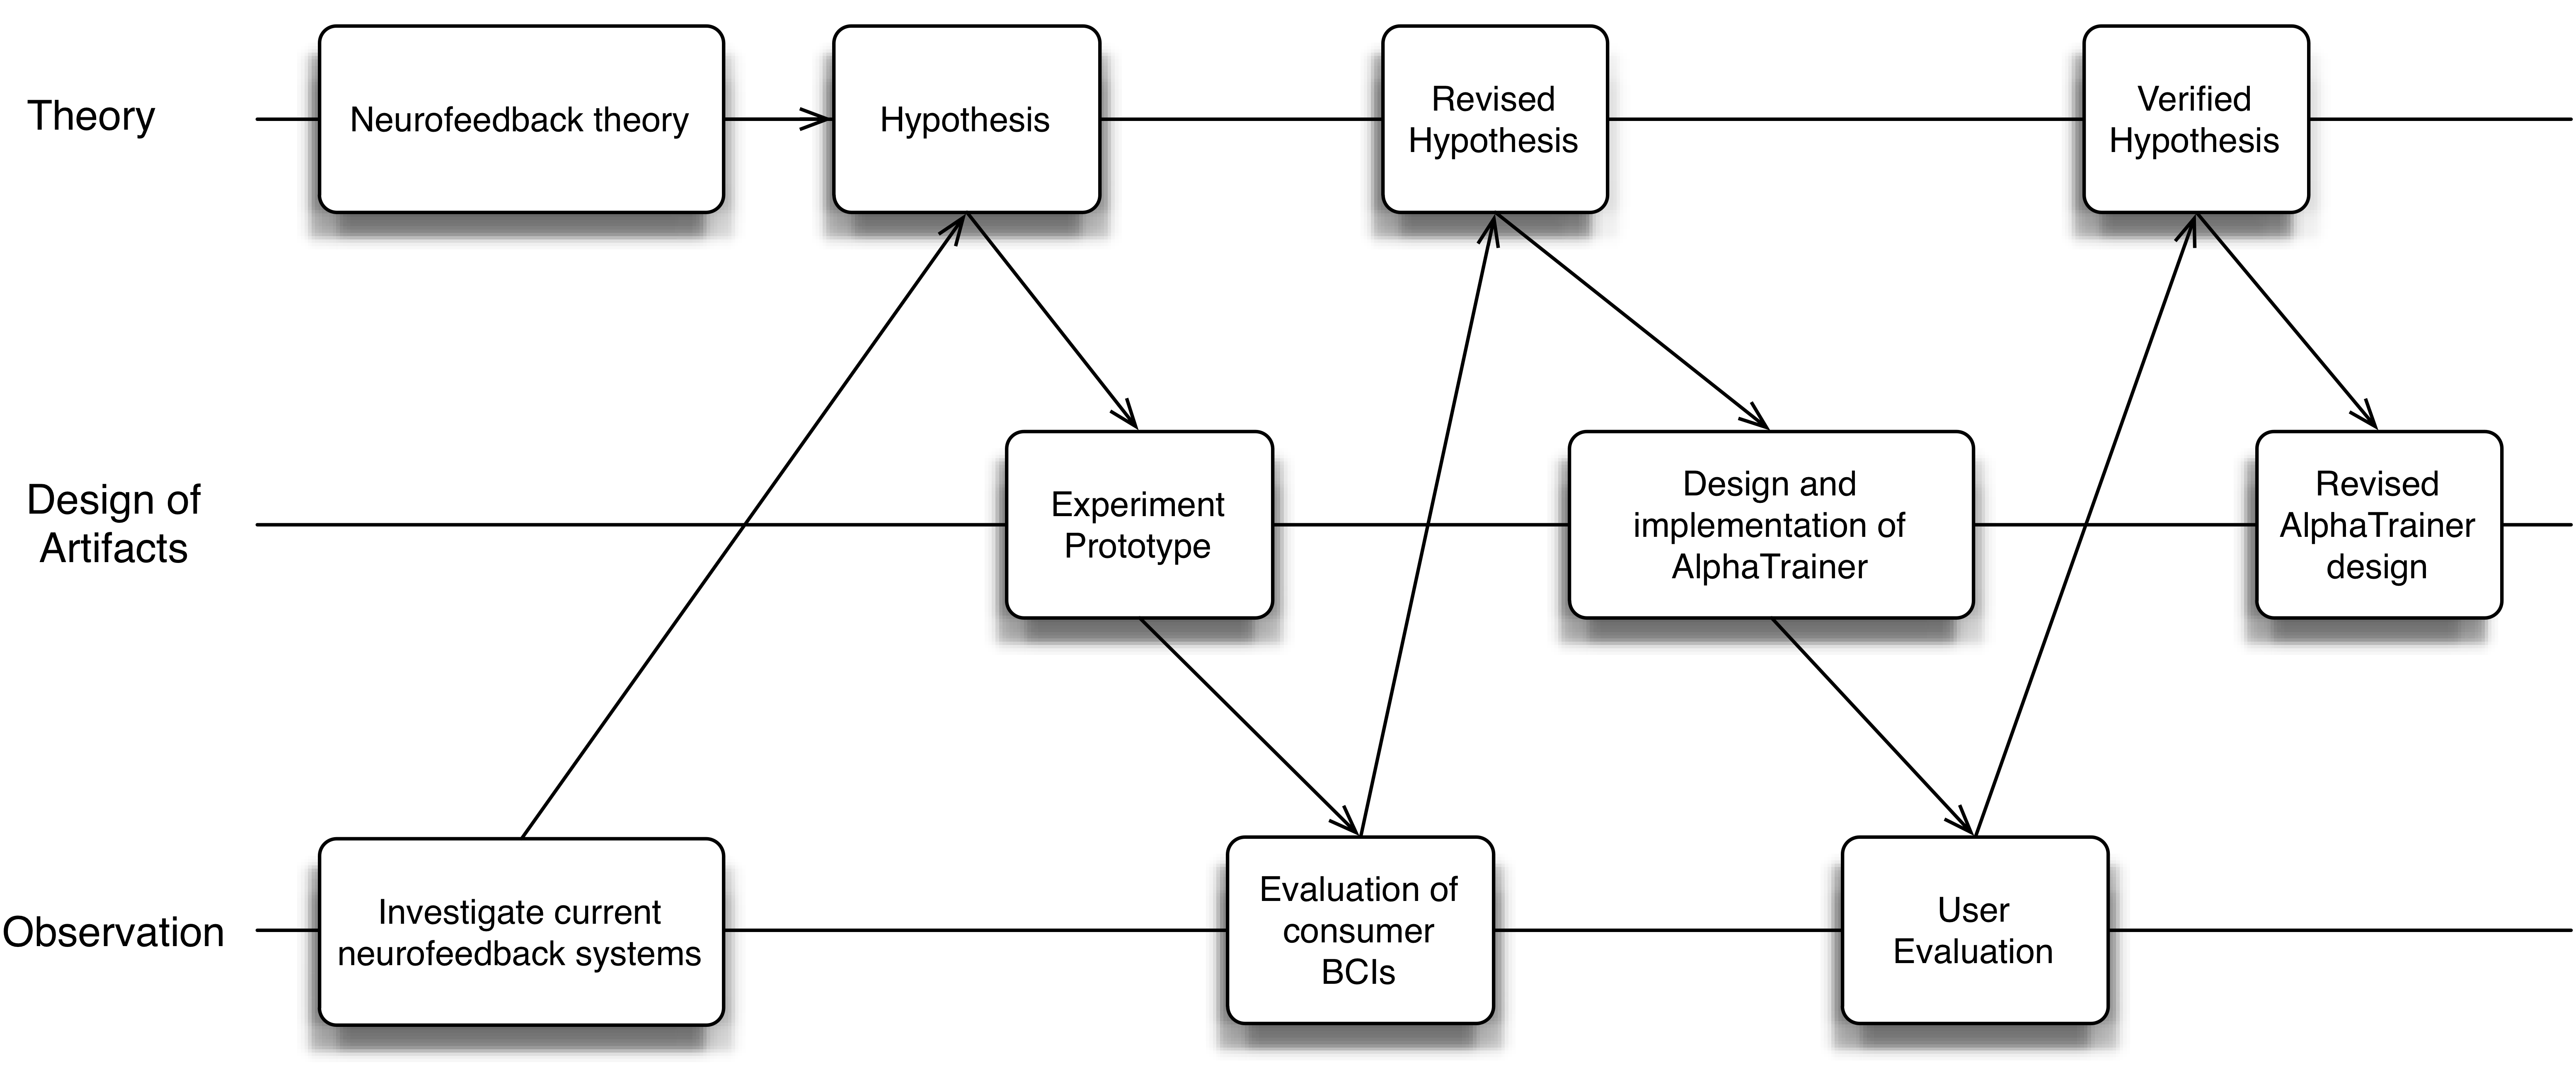
\includegraphics[width=1.000\linewidth]{triangulation.png}
\caption[Mapping of activities in the thesis activities and process]{Mapping of the thesis activities and process - applying the triangulation
framework proposed by Mackay and Fayard \cite{mackay_hci_1997}.}\label{ch-intro/index:fig-triangulation}\end{figure}


\section{Thesis overview}
\label{ch-intro/index:ch-intro-thesis-overview}\label{ch-intro/index:thesis-overview}
We outline the structure of this thesis below based on the thesis activities
mapped in Figure \ref{ch-intro/index:fig-triangulation}.

In Chapter {\hyperref[ch-background/index:ch-background]{2}} we establish a broad overview of
BCIs and neurofeedback training. The chapter describes related consumer
products and related works within the area of consumer BCIs and
neurofeedback. This is the foundation of our hypothesis and it frames
\emph{Neurofeedback theory} and \emph{Investigate current neurofeedback systems}.

Chapter {\hyperref[ch-experiment/index:ch-experiment]{3}} describes the design of the \emph{Experimental
prototype} and the \emph{Evaluation of consumer BCIs} within the designed
experiment. This evaluation addresses our first goal - \textbf{G1} (Section {\hyperref[ch-intro/index:ch-intro-hypothesis-goals]{1.2}}). The gained knowledge of the BCIs
capabilities leads us to a \emph{Revised Hypothesis}
which enables us to develop the system design in the next chapter.

The \emph{Design and implementation of AlphaTrainer} is split in two chapters.
Chapter {\hyperref[ch-design/index:ch-design]{4}} outlines the design activities, decisions and
process that lead us to our final design, while Chapter {\hyperref[ch-implementation/index:ch-implementation]{5}} covers the implementation of the AlphaTrainer system.

In Chapter {\hyperref[ch-evaluation/index:ch-evaluation]{6}} we evaluate the system through a
\emph{User Evaluation of AlphaTrainer}. The chapter addresses directly our
second goal - \textbf{G2} (Section {\hyperref[ch-intro/index:ch-intro-hypothesis-goals]{1.2}}) and leads
us to a \emph{Verified Hypothesis} and a \emph{Revised AlphaTrainer design}.

Finally we make out the conclusion and outline future works - Chapter {\hyperref[ch-conclusion/index:ch-conclusion]{7}}.


\section{Limitations}
\label{ch-intro/index:ch-intro-limitations}\label{ch-intro/index:limitations}
This thesis does not attempt to make any clinical claims about AlphaTrainer's
efficacy regarding stress treatment. Nor does it address the security aspects
of data management which would be required for a system for clinical use.

Rather, it explores whether a neurofeedback system can actually be build
using a mobile device and a low-cost consumer BCI. Furthermore, it explores
through real world deployment of a prototype whether it makes sense for users
to perform neurofeedback training in an everyday context.


\chapter{Background}
\label{ch-background/index:ch-background}\label{ch-background/index::doc}\label{ch-background/index:background}
In this chapter we start out briefly explaining what EEG is and how a
Brain-Computer Interface (BCI) works including typical approaches to data
processing and classical applications. We then move on to describe relevant
consumer BCIs. Finally, we outline neurofeedback training and how it relates to
stress reduction. We conclude the chapter with an overview of neurofeedback
systems which are either aimed at consumers or using consumer BCIs.


\section{BCI / EEG}
\label{ch-background/index:bci-eeg}
The brain consists of billions of neurons. Communication between neurons is
manifested in electrical signals. Electroencephalography (EEG) measures this
electrical activity along the scalp. This is a well established technique from
the 1920s. EEG has a low spatial but a high temporal resolution which makes it
ideal for recording changes in brain activities in response to events. A BCI
takes brain activity - for example in the form of an EEG signal (which is the
case for all BCIs mentioned in this thesis) - as input \cite{tong_quantitative_2009}. For example, Figure \ref{ch-background/index:fig-eeg-with-alpha-waves} shows an EEG signal with visible alpha waves.
\begin{figure}[tbp]
\centering
\capstart

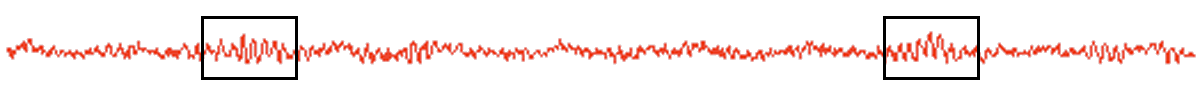
\includegraphics[width=1.000\linewidth]{eeg_wave_with_alpha.png}
\caption[EEG with alpha waves]{EEG signal with alpha waves marked with black boxes.}\label{ch-background/index:fig-eeg-with-alpha-waves}\end{figure}

Brain activity is not the only source of electrical signals along the
scalp. Muscle activation also relies on electrical signals, the measuring of
which is called electromyography (EMG). Eye movement furthermore discharges
electricity due to the eyes dipole properties - measuring this signal is called
electrooculography (EOG). In the context of measuring EEG, EMG and EOG are
typical noise artifacts \cite{majumdar_human_2011}.

EEG is measured either with stand-alone electrodes or electrodes attached to a
cap. Examples of high fidelity EEG BCIs are the \emph{gamma-2-cap} from \emph{g.tec}\footnote{
\href{http://www.gtec.at}{http://www.gtec.at}
} and \emph{Easy Cap} from EASYCAP
\footnote{
\href{http://www.easycap.de/easycap}{http://www.easycap.de/easycap}
}. Some caps can even have up to 256 electrodes
mounted \cite{tong_quantitative_2009}. Caps need mounting preparations
with gel to improve the conductivity between scalp and electrodes. We have tried
out the \emph{gamma-2-cap} during a BCI seminar in Aalborg 2013 (Figure 
\ref{ch-background/index:fig-bci-classic-cap-martin-pelle}). A hi-fi EEG based BCI cost around
10-15.000 Euro and includes, for example, a cap with electrodes, cables
and an amplifier.

The EEG data is usually processed and analyzed off line with tools like EEG-lab \cite{delorme_eeglab:_2004} or FieldTrip \cite{oostenveld_fieldtrip:_2011} which are open-source plug-ins to MATLAB \footnote{
\href{http://www.mathworks.se/products/matlab}{http://www.mathworks.se/products/matlab}
}.
\begin{figure}[tbp]
\centering
\capstart

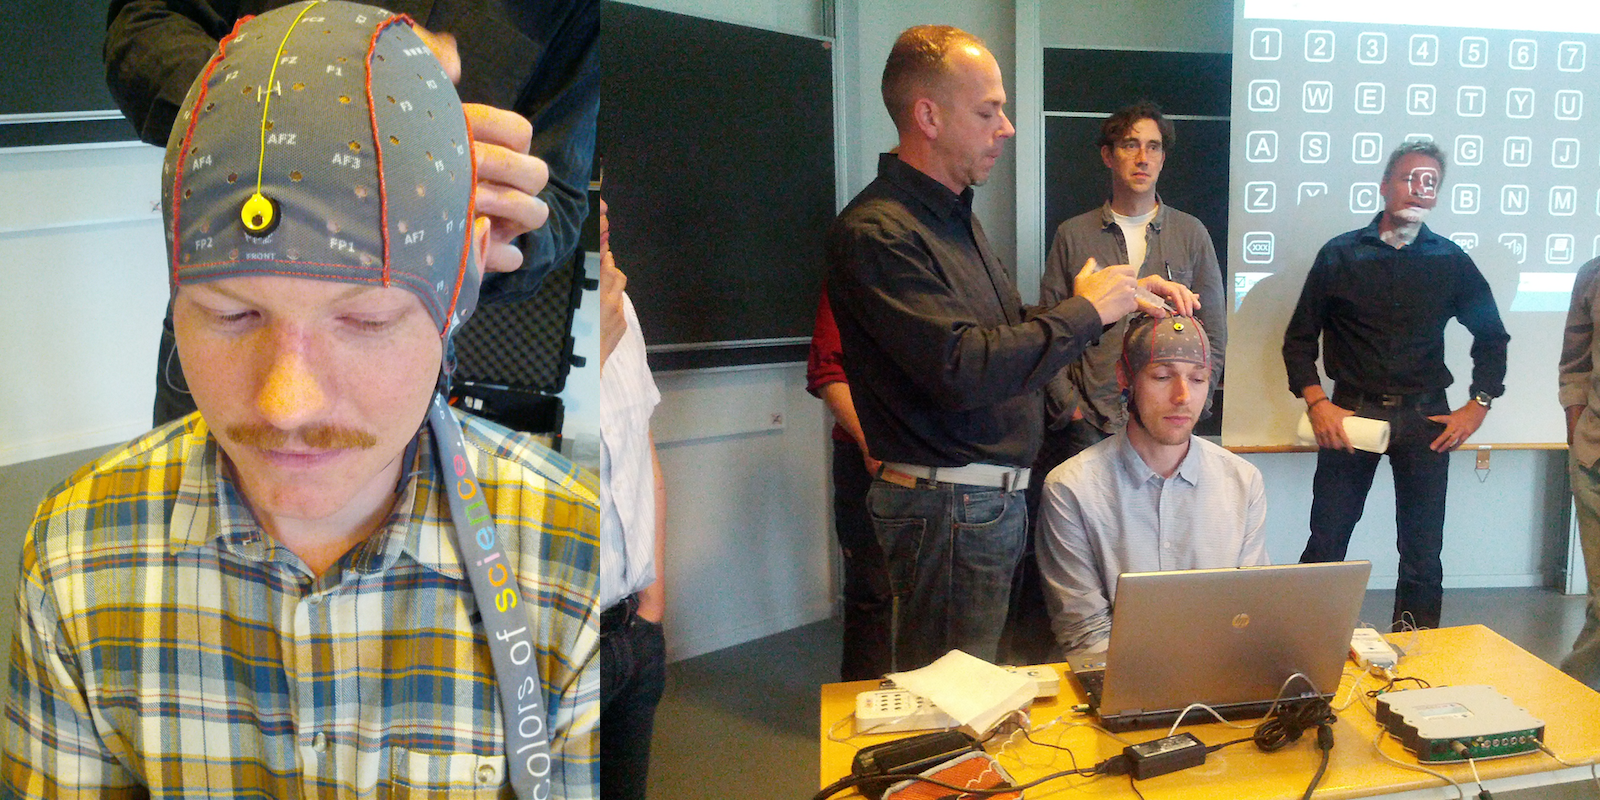
\includegraphics[width=0.700\linewidth]{gcap2_martin_pelle_collage.png}
\caption[Gamma-2-cap]{Martin and Pelle wearing a gamma-2-cap mounted by Gunther Krausz from g.tec}\label{ch-background/index:fig-bci-classic-cap-martin-pelle}\end{figure}


\subsection{Classic BCI applications and techniques}
\label{ch-background/index:classic-bci-applications-and-techniques}
There are different approaches to processing a raw EEG signal. Some of these and
their typical applications are briefly covered below.

Evoked Potentials correlates visual/auditory stimuli with EEG responses. When an
event of significance is perceived, the brain fires certain action
responses. One widely used response is the P300 which manifests itself as a peak
in the EEG signal 300 ms after a stimulus - for example a flash of an image. In
the \emph{intendiX} \footnote{
\href{http://www.gtec.at/Products/Complete-Solutions/intendiX-Specs-Features}{http://www.gtec.at/Products/Complete-Solutions/intendiX-Specs-Features}
} P300 speller application from
\emph{g.tec} different letters are flashed for user while the P300 action response is
used to determine which letter the user wants to select.

Motor imagery is another classic approach to BCI in which an imagined movement
of a body part causes motor cortex activity which is detected by the BCI. In
this way imagined movement can be used for example to control wheel chairs and
other vehicles \cite{mcfarland_brain-computer_2011}. This technique
has been used in gaming as well, e.g. for trigger activation \cite{coyle_eeg-based_2011}. Motor imagery requires spatialization
(localization) of brain activity especially within motor cortex. This
presents a challenge for EEG based BCIs since they have a low spatial
resolution.

Classification of EEG signals are widely used within BCI applications. For
example, it has been used for unique identification of a person for
authentication purpose \cite{schmalstieg_gaze-directed_2010}. Various
research groups uses classifications to predict epilepsy attacks \cite{stam_nonlinear_2005}\cite{meng_feature_2010}. Others do pattern
matching on walking motions for assisting in rehabilitation after strokes
\cite{kuramoto_trigger_2012}. This approach has also been used to classify:
(\emph{i}) emotions like joy and anger; and (\emph{ii}) human expressions like a happy
facial expression or a mental mood  \cite{hutchison_emotional_2011}
\cite{bekkedal_human_2011} \cite{ichi_ito_association_2010}.

\begin{figure}
\centering
\capstart
\begin{subfigure}[t]{0.48\linewidth}
\centering
\capstart

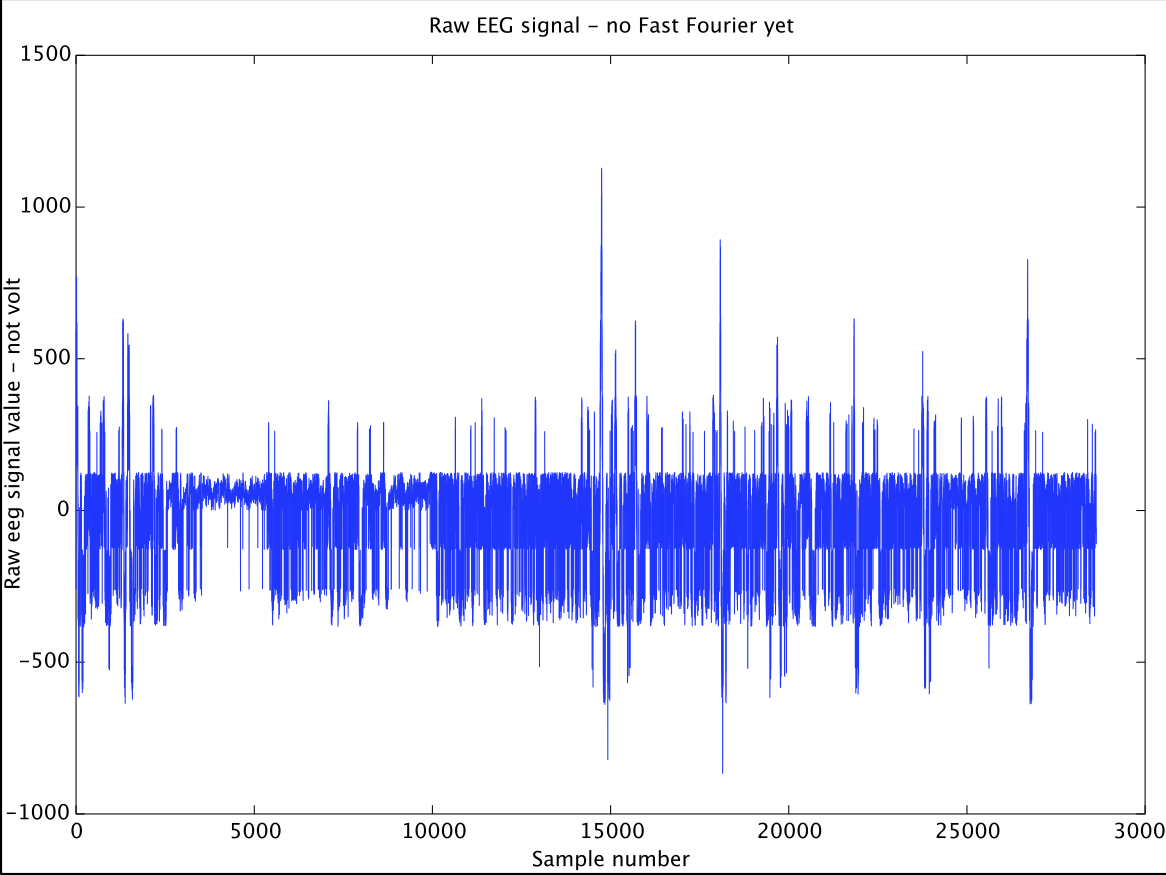
\includegraphics[width=1.000\linewidth]{mindwave_eeg_raw.png}
\caption[Single channel raw EEG]{Single channel raw EEG with 512 samples per second.}\label{ch-background/index:fig-background-mindwave-eeg-raw}\end{subfigure}
\begin{subfigure}[t]{0.48\linewidth}
\centering
\capstart

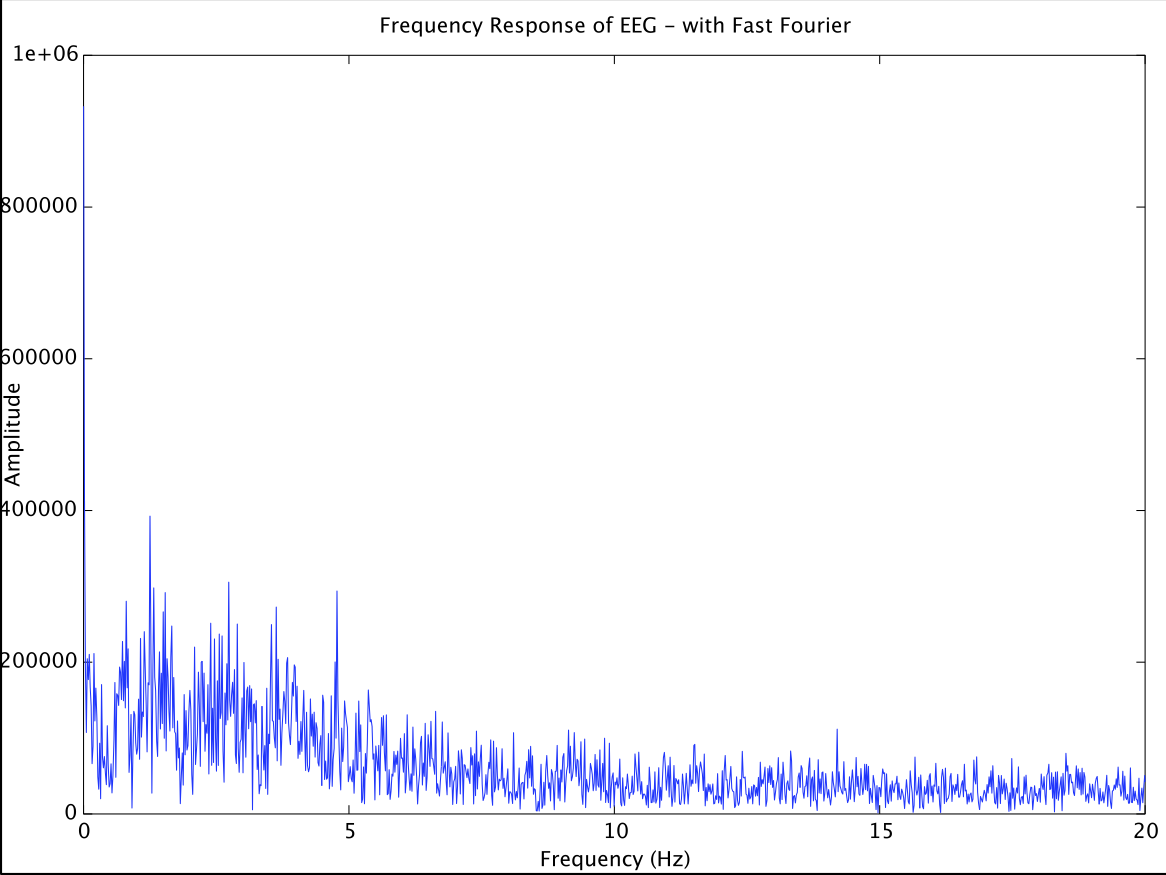
\includegraphics[width=1.000\linewidth]{mindwave_eeg_fft.png}
\caption[Single channel raw EEG applied FFT]{Single channel EEG after Fast Fourier transform (FFT) has been applied.}\label{ch-background/index:fig-background-mindwave-eeg-fft}\end{subfigure}
\caption[Raw EEG and processed EEG]{Raw EEG and Fast Fourier transformed EEG.}\phantomsection\label{ch-background/index:fig-background-eeg-raw-fft}

\end{figure}


Frequency analysis is another technique for processing EEG data.
Neurons are organized in networks and communication among them is always ongoing
in oscillatory patterns. Frequency analysis estimates the power of each
frequency component. One common approach to frequency analysis is to apply Fast
Fourier transform (FFT) - a simple example is plotted in Figure \ref{ch-background/index:fig-background-eeg-raw-fft}. When applying FFT we go from a time domain
into a frequency domain as can be seen on the x-axis values of the plots before
and after FFT. Frequency analysis is often used in conjunction with
other methods of analysis - for example to extract features for classification \cite{tong_quantitative_2009}. It is also used stand-alone either for
neurofeedback or in research aiming to correlate certain frequency patterns with
some condition or cognitive task. This is very typical within EEG research
exemplified by a study showing that ``\emph{... high resting theta power in healthy
older adults is associated with better cognitive function}`` \cite{finnigan_resting_2011}.

Frequency analysis is interesting due to the correlation between frequencies and
mental states \cite{hammond_what_2007} \cite{rangaswamy_beta_2002}. A rough overview is lined up in Table \ref{ch-background/index:table-background-frequency-bands}.


\begin{table}
\capstart
\begin{center}

\begin{tabular}{l l l}

\toprule
\textsf{\relax 
Brainwave Type
} & \textsf{\relax 
Frequency range
} & \textsf{\relax 
Mental states and conditions
}\\
\hline\midrule

\textbf{Delta}
 & 
0.5Hz to 3.5Hz
 & 
Deep sleep
\\

\textbf{Theta}
 & 
3.5Hz to 8Hz
 & 
Falling asleep
\\

\textbf{Alpha}
 & 
8Hz to 12Hz
 & 
Relaxed awake state (dominant with eyes closed)
\\

\textbf{Beta}
 & 
12Hz to 30Hz
 & 
Mental activity, attention, concentration
\\

\textbf{Midrange
Beta}
 & 
16Hz to 20Hz
 & 
Thinking, aware of self \& surroundings
\\

\textbf{High Beta}
 & 
21Hz to 30Hz
 & 
Alertness, agitation
\\

\textbf{Gamma}
 & 
30Hz to 100Hz
 & 
Reflects the mechanism of consciousness
\\
\hline\bottomrule

\end{tabular}
\caption[Generalized frequency bands]{Generalized frequency bands}\phantomsection\label{ch-background/index:table-background-frequency-bands}
\end{center}
\end{table}

The hi-fi BCIs are getting mobile. This trend is exemplified by a mobile version
of the \emph{Easy Cap} and helmets with built in EEG sensors for soldiers \cite{matthews_real_2008}. Another branch of BCIs that have come far in
getting mobile are the consumer BCIs as described in the next section.


\section{Consumer BCIs}
\label{ch-background/index:consumer-bcis}\label{ch-background/index:ch-background-consumer-bcis}
Within recent years consumer BCIs have emerged and moved BCIs outside the
laboratories. An early consumer BCI was the Neural Impulse Actuator (NIA) \footnote{
\href{http://ocz.com/consumer/company/newsroom/news/ocz-announces-availability-of-vista-64-bit-drivers-for-the-nia-neural-impulse-actuator-gaming-peripheral}{http://ocz.com/consumer/company/newsroom/news/ocz-announces-availability-of-vista-64-bit-drivers-for-the-nia-neural-impulse-actuator-gaming-peripheral}
} released in 2008 featuring a three forehead sensor
configuration and connectivity through a desktop box with cables. NIA was
intended primarily for gaming and cost around 100 USD (it is not in production
any longer). Consumer headsets today typically offer additional sensors
(accelerometer, gyroscope, etc) and wireless connectivity.  An overview of
current state consumer BCIs is presented in Table \ref{ch-background/index:table-consumer-bcis}.


\begin{table}
\capstart
\begin{center}

\bodyspacing

\begin{tabular}{>{\raggedright\arraybackslash}p{0.18\linewidth} p{0.14\linewidth} p{0.14\linewidth} p{0.14\linewidth} p{0.14\linewidth} p{0.14\linewidth}}

\toprule
\textsf{\relax 
Feature
} & \textsf{\relax 
Emotiv EPOC (Research)
} & \textsf{\relax 
MindWave Mobile
} & \textsf{\relax 
TrueSense Kit (OPI)
} & \textsf{\relax 
Muse
} & \textsf{\relax 
Emotiv INSIGHT
}\\
\hline\midrule

\textbf{Raw EEG}
 & 
No / Yes
 & 
Yes
 & 
Yes
 & 
Yes
 & 
Yes
\\

\textbf{Electrodes}
 & 
14
 & 
1
 & 
2
 & 
4
 & 
5
\\

\textbf{Locations}
 & 
AF3, F7, F3, FC5, T7,
P7, O1, O2, P8, T8,
FC6, F4, F8, AF4
 & 
--
 & 
--
 & 
AF3, AF4, TP9, TP10
 & 
AF3, AF4, T7, T8, Pz
\\

\textbf{Sensors type}
 & 
Wet
 & 
Dry
 & 
Dry/gel
 & 
Dry
 & 
Dry
\\

\textbf{Sampling rates}
 & 
128Hz
 & 
512Hz
 & 
512Hz
 & 
100-600Hz
 & 
128Hz
\\

\textbf{Protocol}
 & 
USB Dongle
 & 
Bluetooth
 & 
ZigBee
 & 
Bluetooth
 & 
Bluetooth
\\

\textbf{Power}
 & 
12 hours
 & 
6-8 hours (AAA bat.)
 & 
18 hours
 & 
10 hours
 & 
4 hours
\\

\textbf{Off Line recording}
 & 
N/A
 & 
N/A
 & 
Memory chip
 & 
N/A
 & 
microSD card
\\

\textbf{Extra Sensors}
 & 
Gyroscope
 & 
None
 & 
Accelerometer,
temperature
 & 
Accelerometer
 & 
Accelerometer,
magnetometer
\\

\textbf{SDK}
 & 
OSX, Windows
 & 
Android, IOS, Windows,
OSX
 & 
Linux, Windows, OSX
 & 
Android, IOS, Linux,
Windows, OSX
 & 
Android, IOS, Linux,
Windows, OSX
\\

\textbf{Price}
 & 
300/750 USD
 & 
100 EURO
 & 
40 EURO
 & 
269 EURO
 & 
300 USD
\\

\textbf{Released}
 & 
2009
 & 
2011
 & 
2013
 & 
Ann. 2014
 & 
Ann. 2014
\\
\hline\bottomrule

\end{tabular}
\caption[Listing of consumer BCIs compared by selected features]{Listing of consumer BCIs compared by selected features.}\phantomsection\label{ch-background/index:table-consumer-bcis}
\end{center}
\end{table}

These headsets are interesting to our project. Relevant features and how they
have been used in research is lined out in the next sections.

\begin{figure}
\centering
\capstart
\begin{subfigure}[t]{0.45\linewidth}
\centering
\capstart

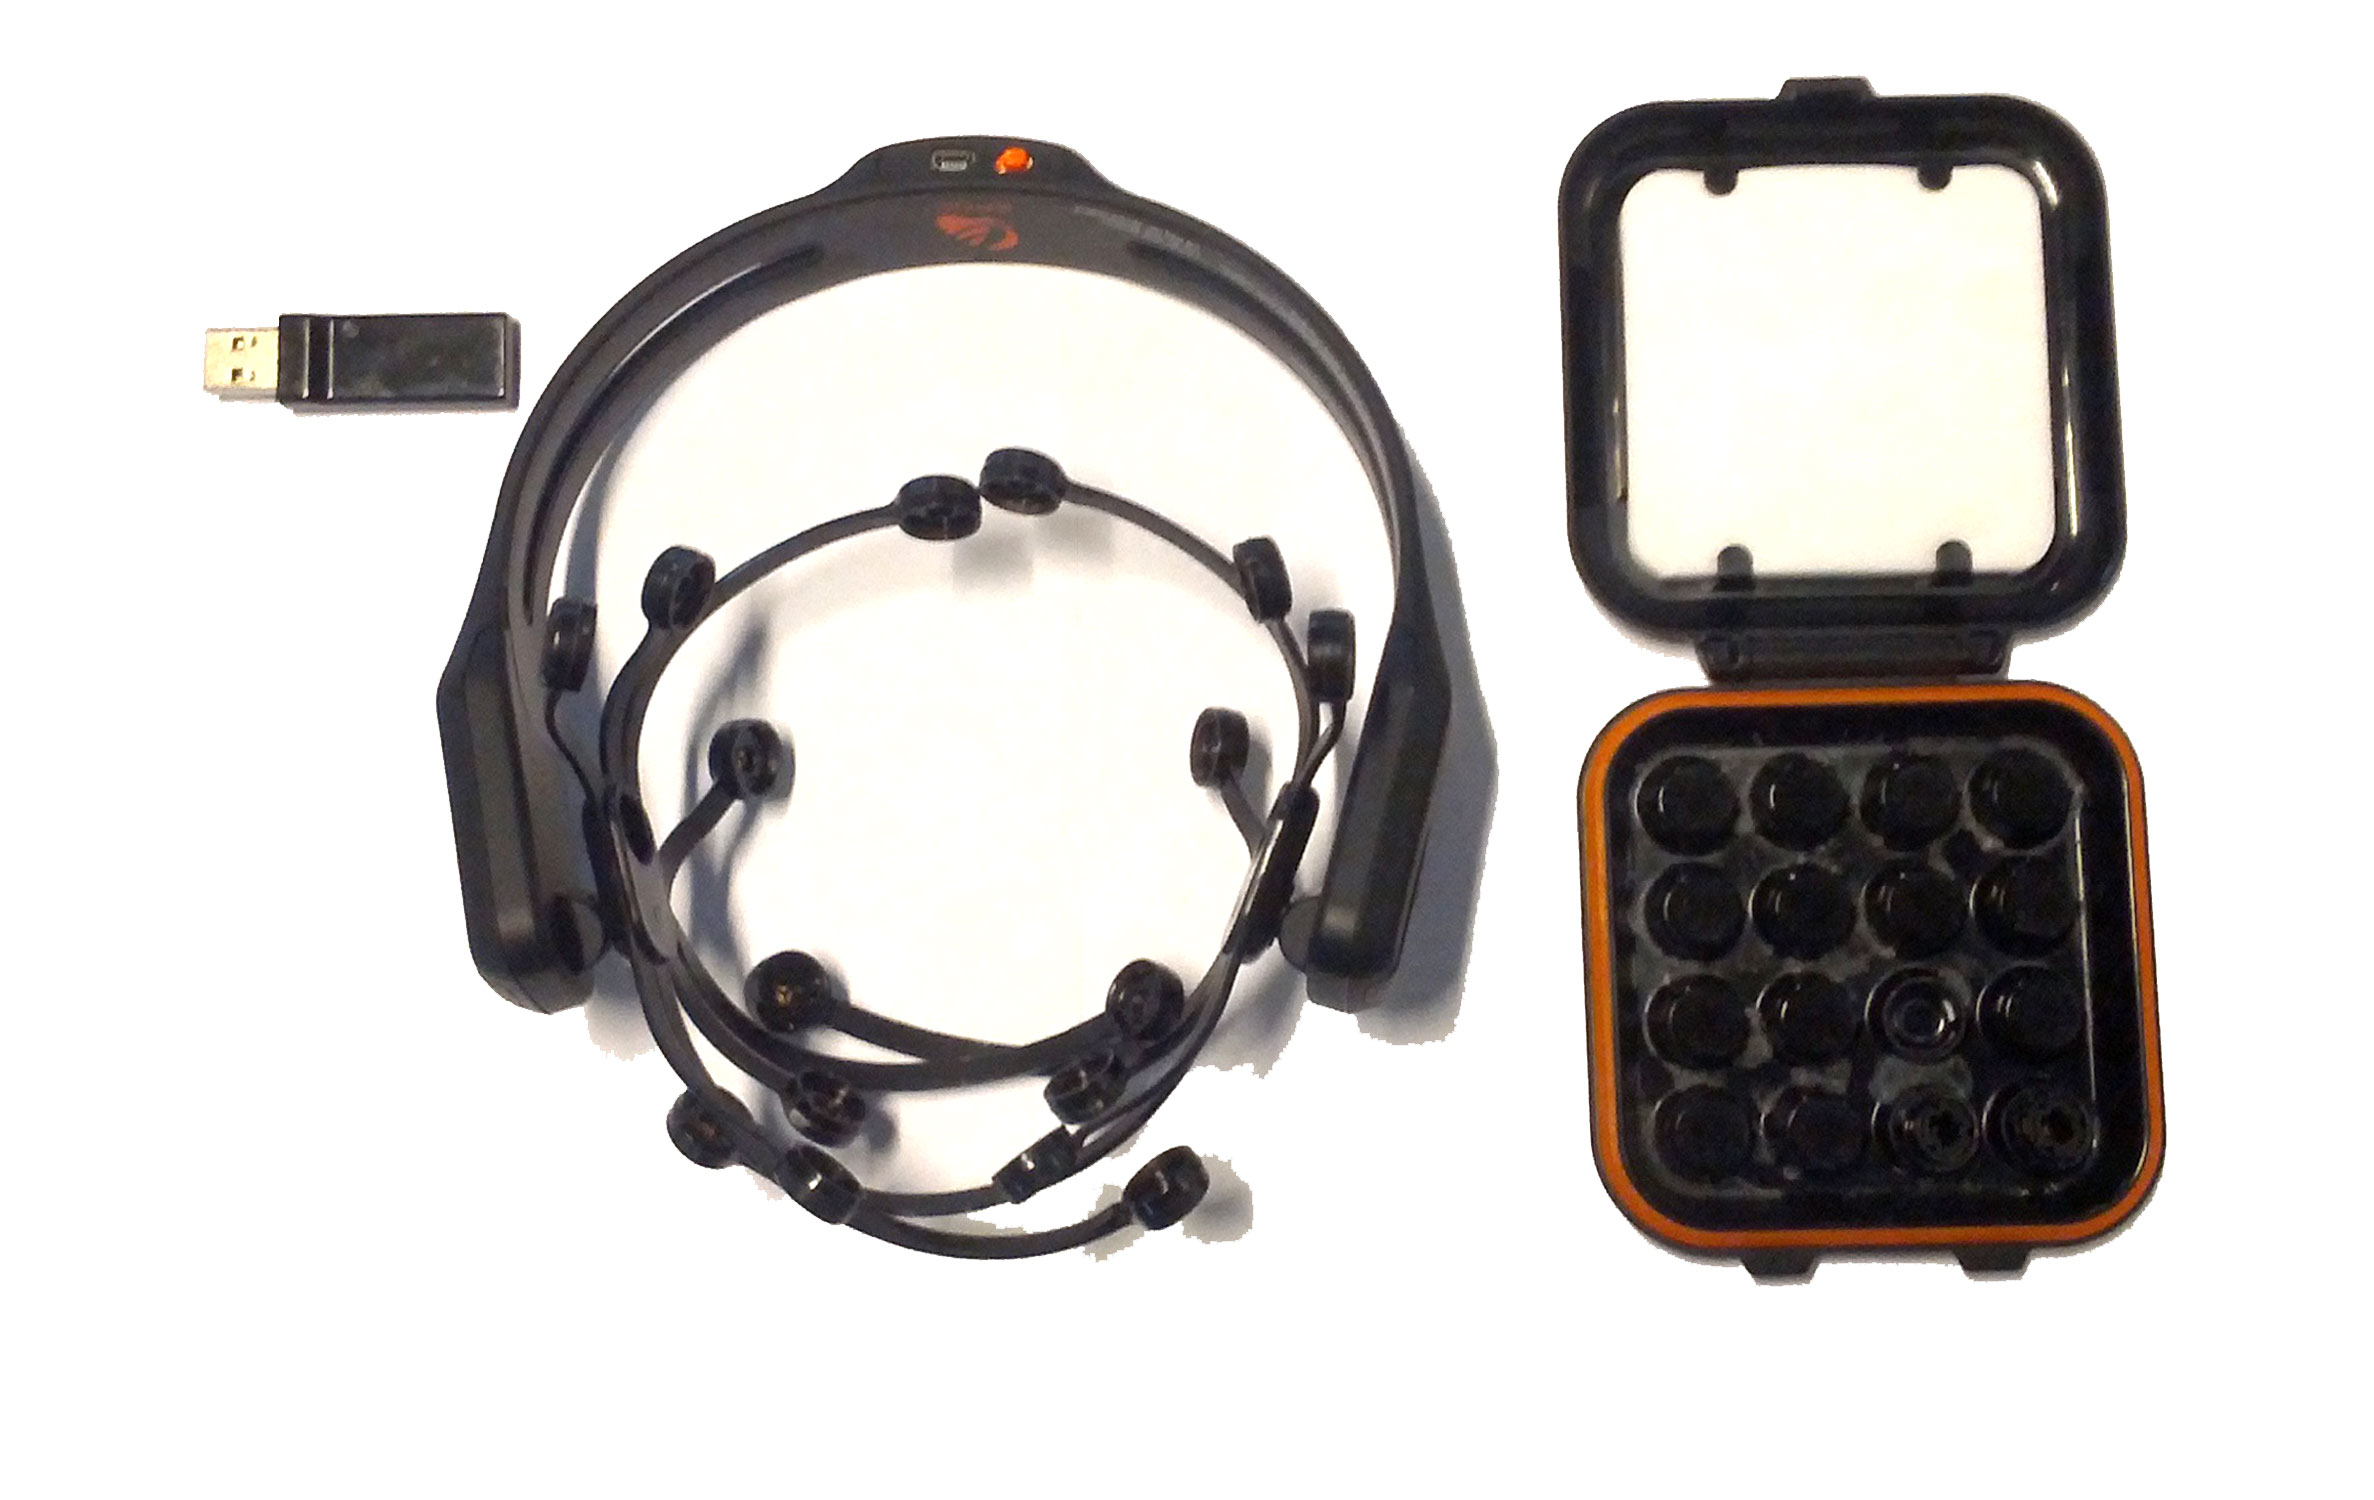
\includegraphics[width=1.000\linewidth]{bci-emotiv-epoc.jpg}
\caption[Emotiv EPOC]{Emotiv EPOC. The image show USB Dongle, electrodes and the EPOC headset}\label{ch-background/index:fig-background-consumer-bcis-epoc}\end{subfigure}
\begin{subfigure}[t]{0.45\linewidth}
\centering
\capstart

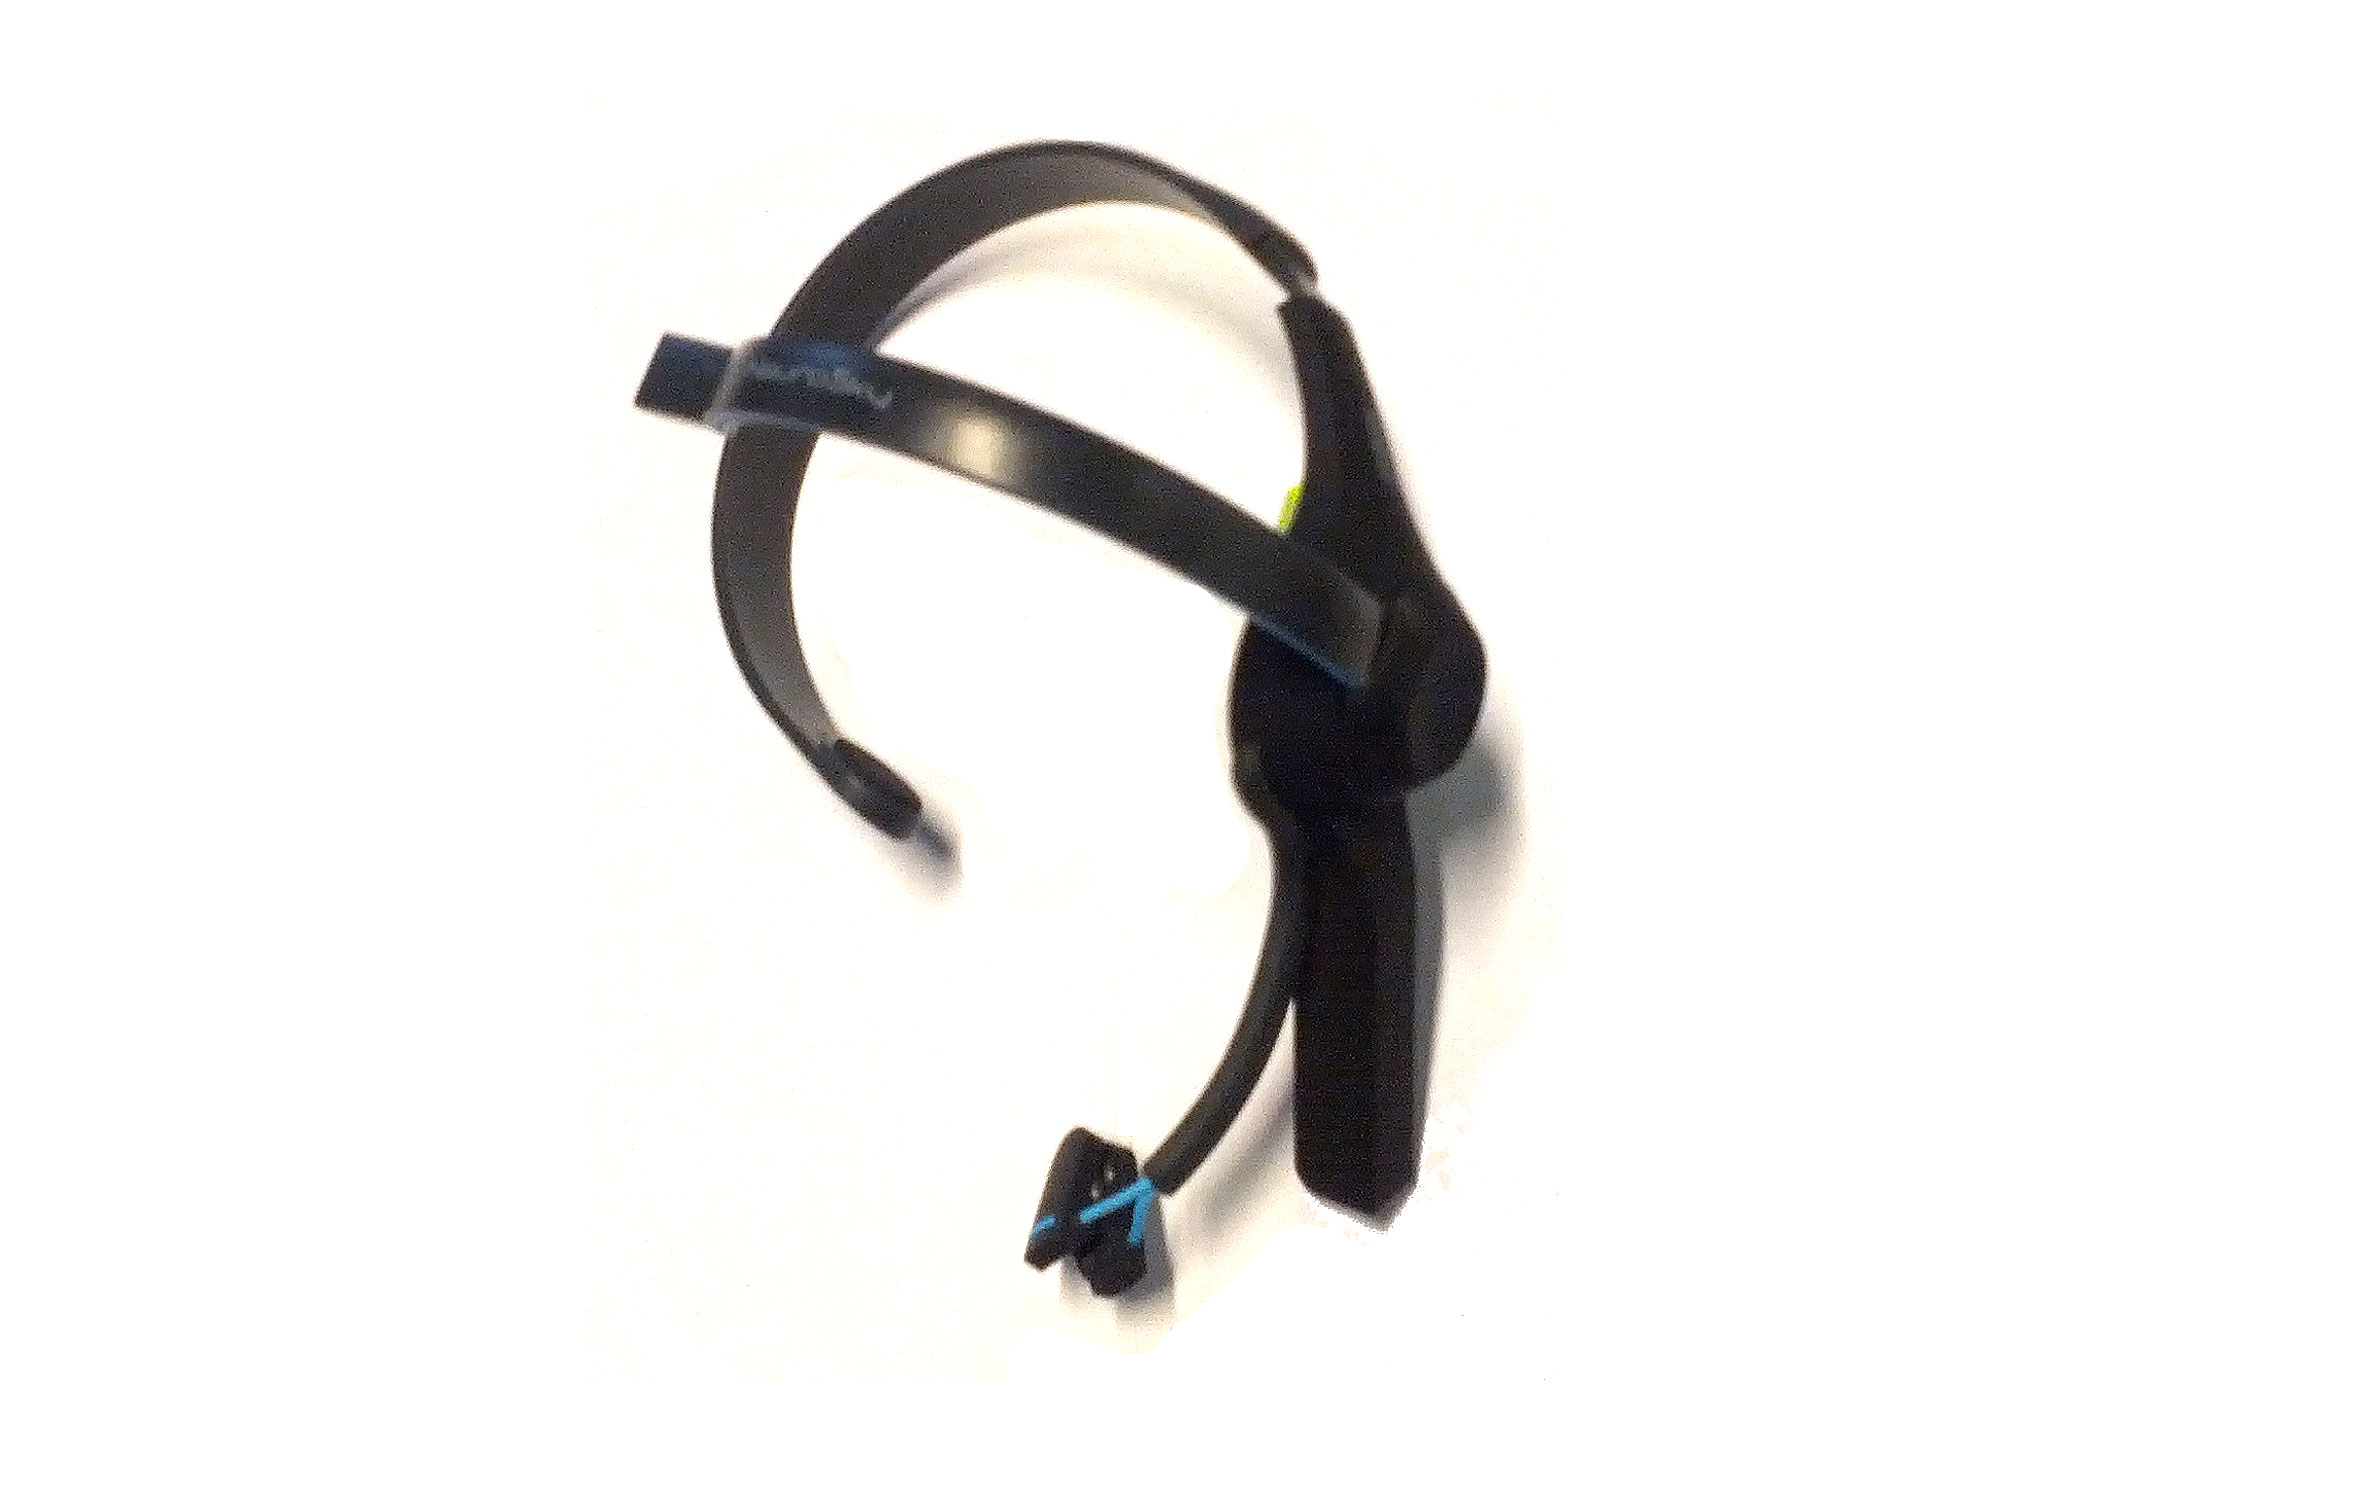
\includegraphics[width=1.000\linewidth]{bci-neurosky-mindwave-mobile.jpg}
\caption[NeuroSky MindWave Mobile]{NeuroSky MindWave Mobile headset.}\label{ch-background/index:fig-background-consumer-bcis-mindwave}\end{subfigure}
\begin{subfigure}[t]{0.45\linewidth}
\centering
\capstart

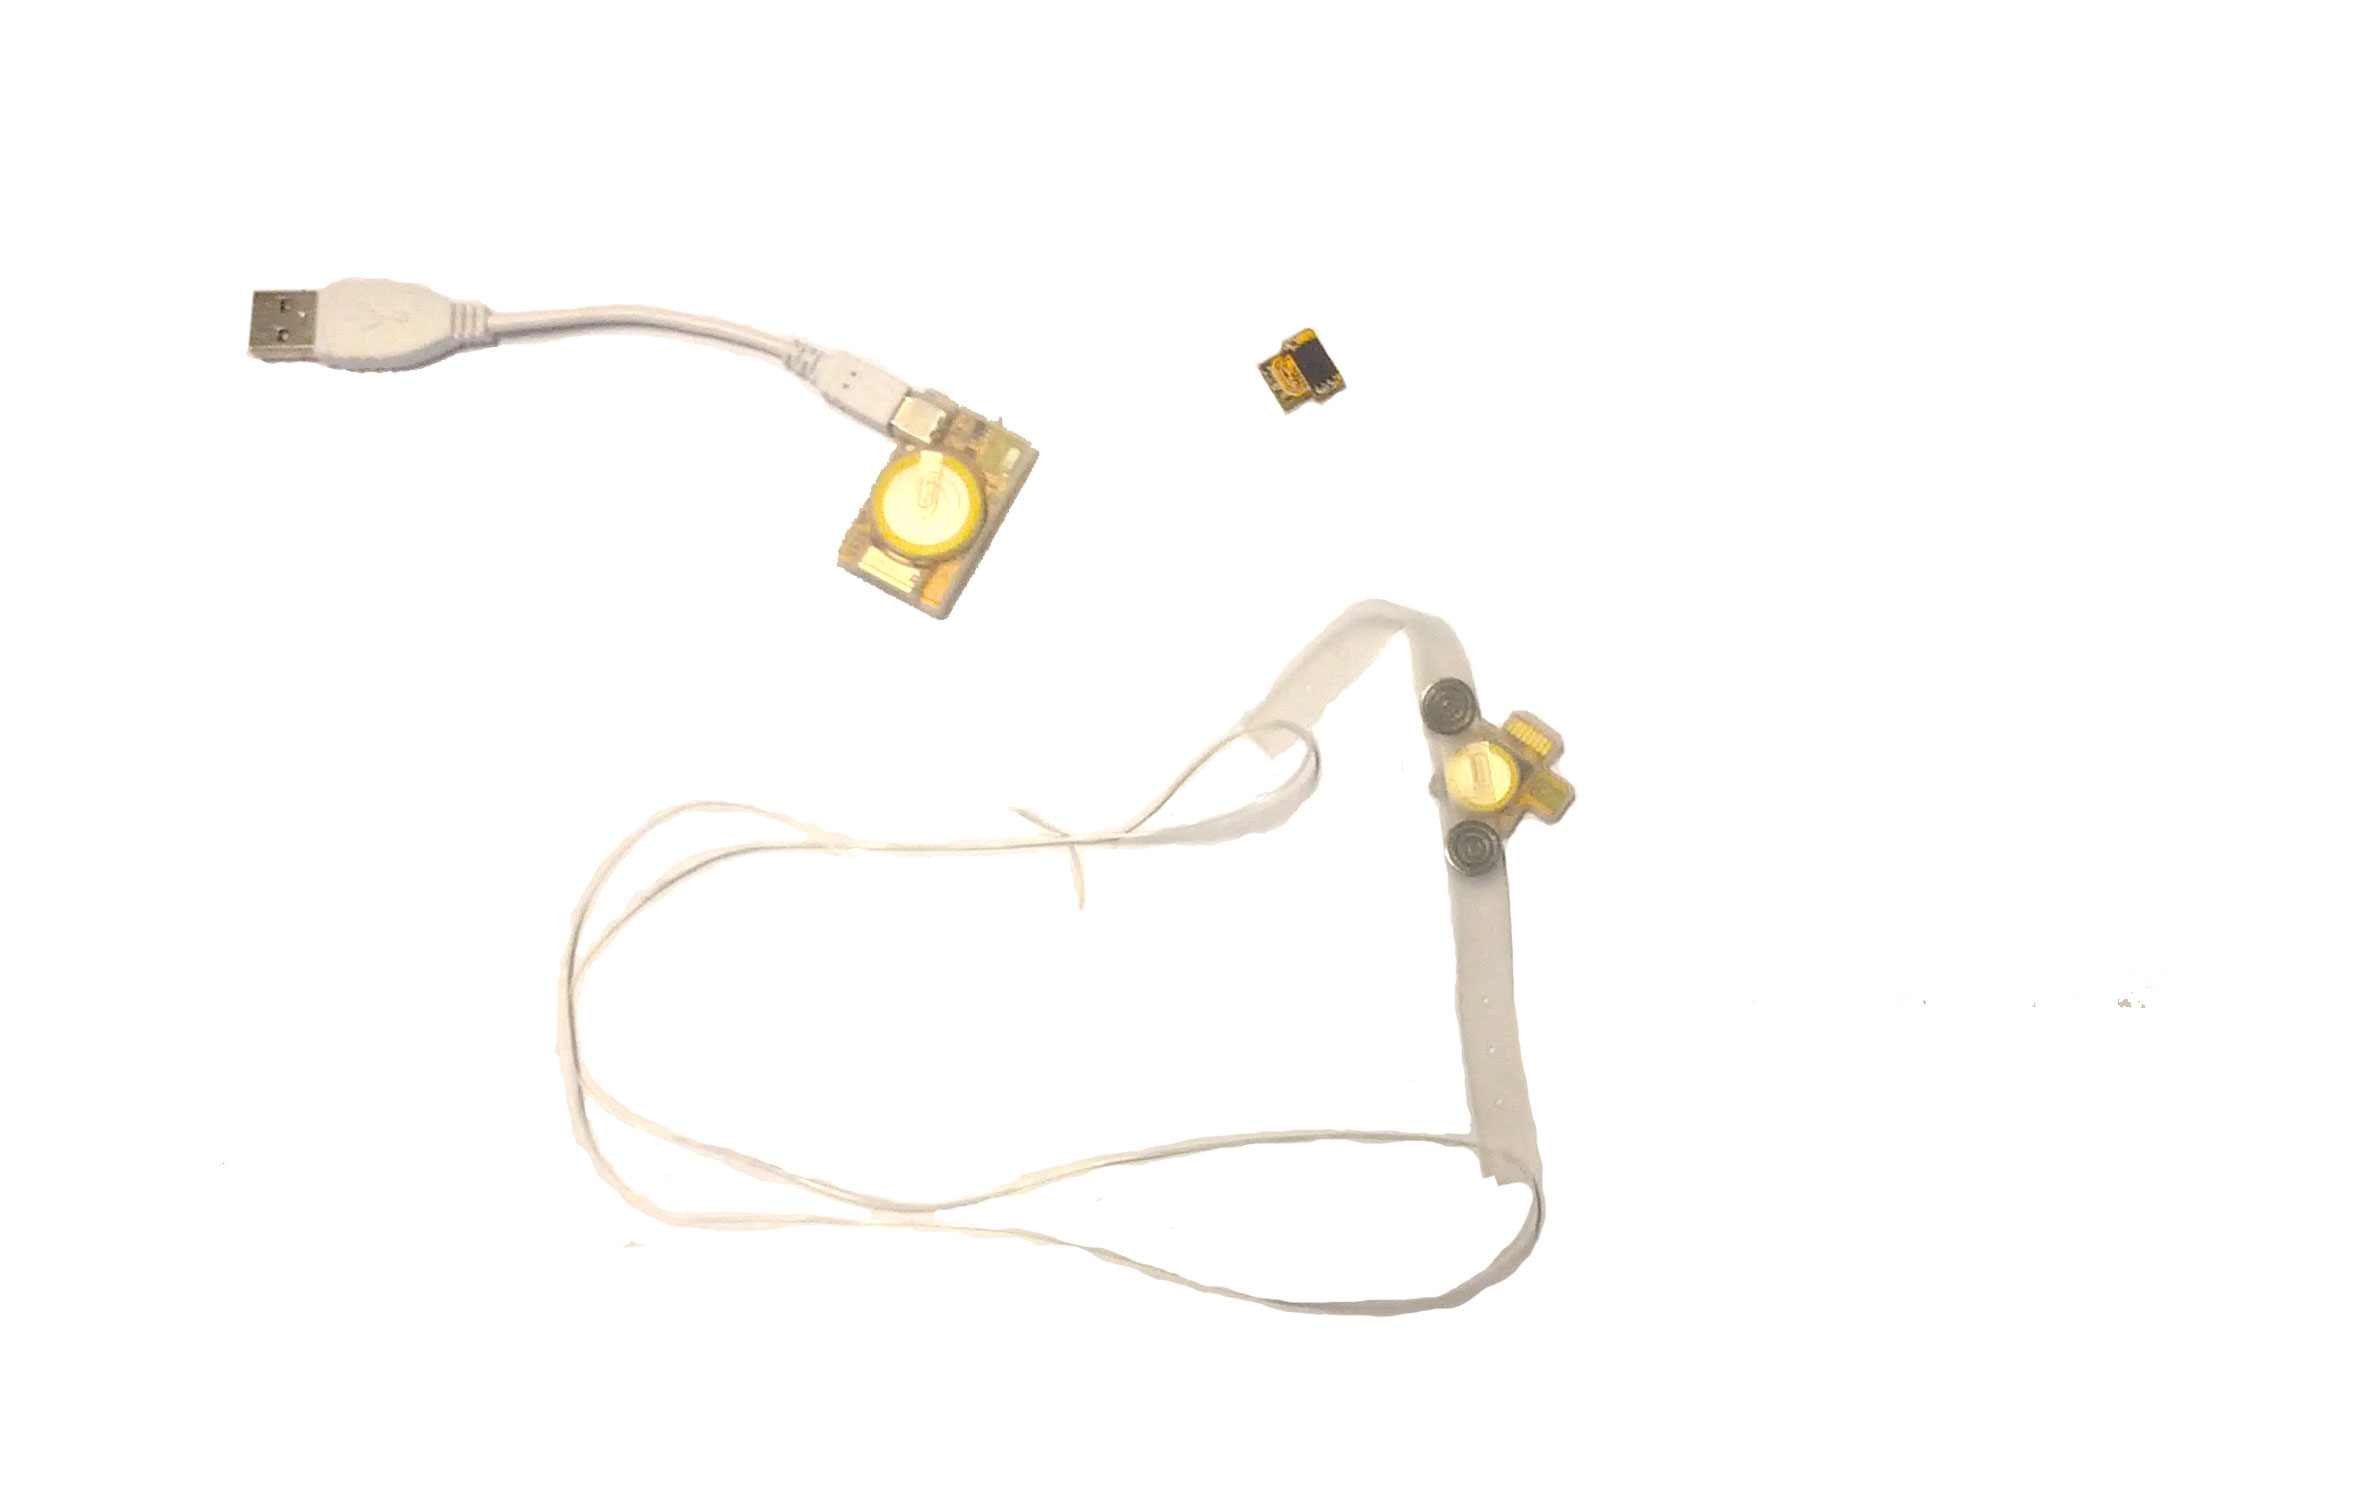
\includegraphics[width=1.000\linewidth]{bci-truesense-kit.jpg}
\caption[TrueSense Kit]{TrueSense Kit. The image show USB controller (w. ZigBee receiver), memory module and TrueSense sensor band.}\label{ch-background/index:fig-background-consumer-bcis-truesense}\end{subfigure}
\caption[Images of consumer BCIs]{Images of 3 consumer BCIs.}\phantomsection\label{ch-background/index:fig-background-consumer-bcis-images}

\end{figure}



\subsection{Emotiv EPOC}
\label{ch-background/index:emotiv-epoc}\label{ch-background/index:fig-background-consumer-bcis-images}\label{ch-background/index:ch-background-epoc}
EPOC has out of the box a desktop SDK and a set of tools aimed at gaming. The
closed source SDK provides detection of emotions, expressions, cognitive states
and more \footnote{
\href{http://emotiv.com}{http://emotiv.com}
} (Figure \ref{ch-background/index:fig-background-consumer-bcis-epoc}).

There is also a research edition of the EPOC headset which can record raw
EEG. It comes with the \emph{TestBench} desktop application for
recording and viewing the raw EEG data. TestBench can process EEG into
various frequency bands and the raw EEG data can be exported in an EDF-format
(multichannel biological and physical signals) \footnote{
\href{http://www.edfplus.info}{http://www.edfplus.info}
} (Appendix {\hyperref[appendix_background_testbench:appendix-background-testbench]{\emph{Emotiv EPOC TestBench}}}).

Before using the EPOC headset, the user has to moist each of its 14 electrode in
a saline solution and then attach each electrode to the headset. This
preparation took us about 10-15 minutes when some routine was achieved.

The EPOC has no SDK for mobile devices, but has been hacked for mobile usage in
conjunction with the USB dongle - we return to this in Section {\hyperref[ch-background/index:sec-related-works]{2.4}}.

EPOC seems to be the consumer BCI that appears most frequently in research
papers. An overview of its application within research is given below.

The \emph{FlyingBuddy2} uses motor imagery to make it possible for a disabled person
to steer a Drone with the future perspective of steering a wheel chair \cite{yu_flyingbuddy2:_2012}. A group in Spain uses the out of the box SDK
classified facial expression (based on EMG) such as open and close clinch
combined with EOG data to steer a tractor \cite{gomez-gil_steering_2011}. Again using SDK classifications, an emotion
based chat application has been build featuring avatars that changes their
expression from angry to happy based on the emotional state of a person \cite{wright_emochat_2010}. In a recent M.Sc. thesis the EPOC was used for a
brain wave biometrics authentication system \cite{petersen_development_2012}. The \emph{NeuroPhone} project used a P300
approach to make phone calls on a smart phone - however the EEG processing was
performed on a laptop \cite{campbell_neurophone:_2010}. Finally, EPOC
has also been used in a human-robot interaction study where they used EEG to
classify human satisfaction of the interaction with a robot \cite{esfahani_using_2011}.

EPOC has also been used by media researchers at the Danish
Broadcasting Corporation (DR) as a supplemental tool to qualitative interviews
and questionnaires. Throughout the video screening of a TV Drama production,
the screening participants' brain states were measured in terms of EPOC SDK
values such as excitement, frustration and attention. In an
interview with Harddisken (a DR radio program about technology), Jacob Lyng
Wieland - in charge of the experimental usage of BCI during video screenings -
reported that they had skipped using the EPOC headset because it was too
cumbersome to use \footnote{
\href{http://www.dr.dk/radio/player/ondemand/legacybyrid/1588020\#!}{http://www.dr.dk/radio/player/ondemand/legacybyrid/1588020\#!}
}.


\subsection{NeuroSky MindWave Mobile}
\label{ch-background/index:neurosky-mindwave-mobile}\label{ch-background/index:ch-background-mindwave}
NeuroSky MindWave Mobile (MindWave) \footnote{
\href{http://www.neurosky.com/products/mindwavemobile.aspx}{http://www.neurosky.com/products/mindwavemobile.aspx}
} offers
desktop and mobile SDKs (IOS and Android). The closed source SDK features
frequencies processing and analysis outputting values for the level of
``attention'' and ``meditation'' \cite{neurosky_brain_2009} (Figure \ref{ch-background/index:fig-background-consumer-bcis-mindwave}). The SDK also provides information
about eye blinks and a number of frequency bands which we previously have lined
out in Figure \ref{ch-background/index:table-background-frequency-bands}. The
MindWave SDK outputs the following frequency bands: delta (0.5 - 2.75Hz), theta (3.5 - 6.75Hz),
low-alpha (7.5 - 9.25Hz), high-alpha (10 - 11.75Hz), low-beta (13 - 16.75Hz),
high-beta (18 - 29.75Hz), low-gamma (31 - 39.75Hz) and mid-gamma (41 - 49.75Hz) \cite{neurosky_thinkgear_2012}.

The headset is easy to use and the SDK includes a simple Bluetooth API that
seamlessly supports device connectivity. Due to its connectivity options and SDK
signal processing, the MindWave Mobile requires little effort to embed in a
prototype. This has been done, for example, in a recent paper by Marchesi.
He uses MindWave in the
BRAVO project to detect attention among school children in an e-learning
setting. If a child's attention level is under some threshold, it its reported
to the other children who are encouraged to offer their help \cite{marchesi_bravo:_2013}. In another study, a research group uses
MindWave to measure
attention during an online game. They specifically look at the attention
levels provided by the SDK versus self reported attention levels among a group of
participants. They conclude that the self reports and the SDK values are correlated \cite{hutchison_assessing_2009}. Another paper uses the attention and
meditation SDK values to examine the stress levels among participants while
performing various tasks. It concluded that the
MindSet \footnote{
The experiment used a MindSet headset (the generation before
MindWave but with the same chipset and electrode) \cite{crowley_evaluating_2010}.
} was able to measure an increase in stress
induced by the tasks performed (Stroop test, Tower of Hanoi) \cite{crowley_evaluating_2010}.
In \cite{yasui_brainwave_2009}
the brain state - defined in terms
of EEG frequency composition - of a test subject driving a car is measured by
a predecessor to the MindWave. Raw EEG data is recorded to a mobile phone via
bluetooth and its frequency composition is analyzed offline.
Interestingly, the results show a change in the brain wave frequency pattern
when the driver performed, for example, a phone call.
Finally, in a M.Sc. thesis, classification of the raw EEG data from the MindSet
is used to control a snake-like game aimed at children \cite{larsen_classification_2011}.

MindWave comes out of the box with a mobile application named \emph{Brainwave
Visualizer} which let its user inspect the current levels of the 8 frequency
bands supported by the SDK. The app also provides simple neurofeedback by
letting its user control the flying height of a ball by the SDK ``meditation''
value or the intensity of a flame by the SDK ``attention'' value. The same
approach to neurofeedback is used in the third party app \emph{Transcend} by Personal
Neuro. During meditation the user can get a flower to grow by increasing the
``meditation'' SDK value \footnote{
Android app: \href{https://play.google.com/store/apps/details?id=com.personalneuro.transcend}{https://play.google.com/store/apps/details?id=com.personalneuro.transcend}
}.


\subsection{TrueSense Kit}
\label{ch-background/index:ch-background-truesense-kit}\label{ch-background/index:truesense-kit}
TrueSense Kit is the newest, cheapest, most portable headset. It comes with OPI
Console, an open source desktop application for recording and viewing raw EEG
data and analyzing sleep, meditation etc. from recorded EEG. It also enables exporting data as
EDF-files for further processing and analysis in other applications. The OPI
Console also offers sleep analysis and yoga performance analysis \footnote{
\href{http://op-innovations.com}{http://op-innovations.com}
} (Figure \ref{ch-background/index:fig-background-consumer-bcis-truesense}, Appendix {\hyperref[appendix_background_truesense_console:appendix-background-truesense-console]{\emph{TrueSense Kit console}}}). The TrueSense Kit sensor(s) can
be placed on various parts of the body for measuring blood flow, heart rate, body
temperature and body movements.

TrueSense Kit records either directly to an internal memory module or transmit
data over ZigBee radio to the OPI Console through a USB receiver. The sensors
can be combined in a multi sensor configuration attached various places on the
head or body.

TrueSense Kit provides no immediate mobile device connectivity but the OPI Console
application can likely be ported to Android since it is build with the QT
framework \footnote{
\href{http://qt-project.org}{http://qt-project.org}
}. Another approach would be to build a
native C++ Android module from the TrueSense Kit C++ SDK. Since few Android
devices currently support ZigBee out of the box, this would require an
external receiver board.

TrueSense Kit is not yet covered in any papers despite its support for flexible
experimental setups. TrueSense Kit was warmly received by the quantified self
community at the yearly QS conference in Amsterdam 2013 \footnote{
\href{http://quantifiedself.com/conference/Amsterdam-2013}{http://quantifiedself.com/conference/Amsterdam-2013}
}.


\subsection{Future headsets}
\label{ch-background/index:ch-background-future-headsets}\label{ch-background/index:future-headsets}
New consumer BCIs are about to arrive, for example \emph{Muse} \footnote{
\href{http://www.interaxon.ca}{http://www.interaxon.ca}
} (as briefly mentioned in the Introduction Section {\hyperref[ch-intro/index:ch-intro-neurofeedback-stress-and-bci]{1.1}}) and \emph{Emotiv INSIGHT} \footnote{
\href{http://www.kickstarter.com/projects/tanttle/emotiv-insight-optimize-your-brain-fitness-and-per}{http://www.kickstarter.com/projects/tanttle/emotiv-insight-optimize-your-brain-fitness-and-per}
}. These new headsets have some characteristics in
common which seem to be representative for the new generation of consumer BCIs:
\begin{itemize}
\item {} 
they support Bluetooth

\item {} 
they use dry electrodes

\item {} 
they are discrete and comfortable to wear

\end{itemize}

An interesting fact is that both of these headbands are
crowdfunded. Muse raised 287,472 USD in 2012 from an unknown amount of
supporters at Indiegogo \footnote{
\href{http://www.indiegogo.com/projects/muse-the-brain-sensing-headband-that-lets-you-control-things-with-your-mind}{http://www.indiegogo.com/projects/muse-the-brain-sensing-headband-that-lets-you-control-things-with-your-mind}
}. EPOC Insight had
pledged 1,643,117 USD by the end of September 2013 from nearly 5000 people on
Kickstarter \footnote{
\href{http://www.kickstarter.com}{http://www.kickstarter.com}
}. This trends an interest in
low cost consumer BCIs and exemplifies pretotyping by presenting and selling the
product before it has actually been build \cite{jeremy_pretotypingwork_2012}.

Most importantly, these new BCIs strengthen the possibility for neurofeedback
among consumers in their daily settings. In the next section we focus on the
neurofeedback concept.


\section{Neurofeedback}
\label{ch-background/index:neurofeedback}
When given real time feedback on its oscillations, the brain can learn to
control and change them. This is interesting since the brains oscillations are
significantly correlated with brain functions and behavior as well as with
psychiatric diseases \cite{zoefel_neurofeedback_2011}. Neurofeedback
training exploits this mechanism by providing feedback based on oscillation
frequencies correlated with some desirable function or behavior.

The neurofeedback mechanism was discovered and developed in the 1960s, but the
first controlled studies providing clinical evidence supporting neurofeedback
training effects were published in the 1980s \cite{angelakis_eeg_2007}. Since then, the efficacy of neurofeedback therapy
has been documented in several studies \cite{lofthouse_review_2012} \cite{arns_efficacy_2009} \cite{white_alphatheta_2009} and
neurofeedback \footnote{
a subset of biofeedback which is the term mentioned in the The American
Academy of Pediatrics (AAC) recommendations.
} is listed among the treatments with highest evidence
support for certain conditions according to The American Academy of Pediatrics
(AAP) \cite{_aap_2013}. Neurofeedback is routinely used in
treatment of a number of conditions including Attention Deficit Hyperactivity
Disorder (ADHD), anxiety, epilepsy, and addictive disorders \cite{angelakis_eeg_2007}.

Besides its clinical usage, a number of studies show that neurofeedback training
can increase cognitive performance. For example, it has been shown to increase
semantic working memory,
focused attention, perceptual sensitivity and reaction time \cite{angelakis_eeg_2007}. Neurofeedback training has also been shown
effective by real-life behavioral measures - e.g. by increasing musical
performance in a stressful context among conservatory students in a study
designed to ensure ecological validity \cite{egner_ecological_2003}.


\subsection{Neurofeedback in practice}
\label{ch-background/index:neurofeedback-in-practice}
In a typical clinical context, neurofeedback sessions of 45-60 minutes duration
are performed twice per week. The number of treatments depend on the individual
response to the training and the condition being treated - e.g. 40-80 sessions
are suggested in ADHD treatment \cite{angelakis_eeg_2007}.

Neurofeedback therapy is relatively expensive. For example, 40 training sessions
cost \textgreater{} DKR 30.000,- at Ann-Helen Pettersen's clinic \footnote{
\href{http://www.hjernetraening.dk/prisliste.html}{http://www.hjernetraening.dk/prisliste.html}
}.


\subsection{Stress and alpha feedback training}
\label{ch-background/index:sec-background-stress-alpha-feedback-training}\label{ch-background/index:stress-and-alpha-feedback-training}
Alpha feedback training is the subset of neurofeedback training for
which the goal state of the feedback is defined in terms of the amount
of alpha waves - thereby seeking to increase the alpha activity.

Alpha activity is associated with a relaxed consciousness \cite{angelakis_eeg_2007}. Together with theta, alpha is the EEG
frequency band in which effects of meditation are most significant \cite{aftanas_changes_2003} \cite{brandmeyer_meditation_2013}. Alpha `blocking' (i.e.,
reduction) is associated with alertness \cite{angelakis_eeg_2007}. Thus, by increasing alpha levels, alpha
feedback training has been shown - amongst other positive effects such
as increased cognitive performance - to reduce stress and anxiety \cite{zoefel_neurofeedback_2011} \cite{angelakis_eeg_2007} \cite{white_alphatheta_2009}.

With a classification approach, EEG has been used to classify subjects
from either a chronically stressed or a control group with a success
rate higher than 90\% \cite{khosrowabadi_brain-computer_2011}. This
testifies to the manifestation of stress in EEG data.

The dominant frequency within the alpha band - the \emph{alpha peak} - and the
amplitude of the alpha band varies between individuals \cite{bazanova_comments_2012} \cite{angelakis_eeg_2007} \cite{zoefel_neurofeedback_2011}. An alpha feedback training
system can account for this by calibrating according
to the individual alpha peak and the baseline amount of alpha. This is,
for example, the approach taken in the alpha feedback system presented in \cite{stopczynski_smartphones_2013}. The importance of giving
feedback on individually determined frequency bands is investigated in \cite{bazanova_comments_2012}
and concludes that
``\emph{Neurofeedback training
applied in individual EEG frequency ranges was much
more efficient than neurofeedback training of standard
EEG frequency ranges}''.


\section{Related works}
\label{ch-background/index:related-works}\label{ch-background/index:sec-related-works}
Having explained current state of consumer EEG BCIs, the neurofeedback mechanism
and how alpha feedback training can help to reduce stress, we now present
existing systems and research within the consumer neurofeedback domain. There is
only a limited number of such systems and research for reasons already mentioned
above:
\begin{enumerate}
\item {} 
Neurofeedback therapy is expanding but not widely adopted yet.

\item {} 
Consumer BCIs have only emerged within recent years. They are still maturing and not
widely adopted yet.

\end{enumerate}

This section present and discuss the commercially available systems
Brainball and BioZen and the research project SmartphoneBrainScanner2.


\subsection{Brainball}
\label{ch-background/index:ch-background-brain-ball}\label{ch-background/index:brainball}
According to the researchers behind, Brainball ``\emph{... dwells in the realm between
art and research, entertainment and science, method and object}`` \cite{hjelm_research+_2003}. They present a game with a tangible user
interface in which two opponents sit on a chair separated by a table. A steel
ball lies between them. The players wear specialized BCIs
mounted on their foreheads and somewhat similar to the NIA system (see Section
{\hyperref[ch-background/index:ch-background-consumer-bcis]{2.2}}).
The EEG signal is analyzed into its frequency components and the ball
will roll away from the most relaxed player (drawing on the correlation between
alpha activity and relaxation). While playing, the players are able to see a
screen visualizing their EEG activity. The creators of Brainball interestingly
reports that playing the game leads to increased relaxation by measure of both
Galvanic Skin Response (GSR) and self reports
\cite{hjelm_research+_2003}. Brainball experienced a lot of attention
including honorary mention at Ars Electronica 2000 and 100+ appearances on
TV. However, it remains a niche product within gaming and entertainment due to
the dependency on specialized hardware (BCI, ball, screen, etc). The
Brainball BCI system is commercially available through a Swedish
company under the name \emph{Mindball} \footnote{
\href{http://www.mindball.se}{http://www.mindball.se}
} (Figure \ref{ch-background/index:fig-bci-related-mindball-game}).
\begin{figure}[tbp]
\centering
\capstart

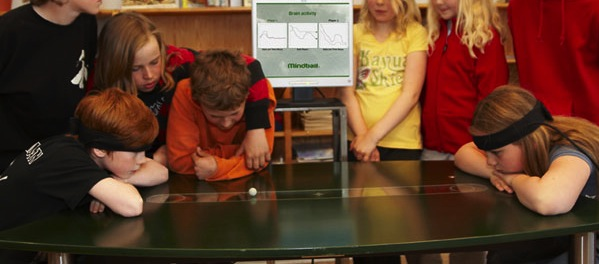
\includegraphics[width=0.800\linewidth]{mindball-game.jpg}
\caption[Mindball game]{Brainball BCI system in the new version named Mindball. A
monitor displays the brain activity of the participants (Image courtesy of
Interactive Productline IP AB).}\label{ch-background/index:fig-bci-related-mindball-game}\end{figure}


\subsection{BioZen}
\label{ch-background/index:biozen}\label{ch-background/index:ch-background-bio-zen}
BioZen \footnote{
\href{http://t2health.org/apps/biozen}{http://t2health.org/apps/biozen}
} is a consumer biofeedback system
developed by the National Center for Telehealth and Technology (T2) under the US
Department of Defense. The fact alone that this organization is behind a
biofeedback system witnesses to the increasing adoptation of the biofeedback
(here under neurofeedback) method. The system consists of an Android application \footnote{
Android App: \href{https://play.google.com/store/apps/details?id=com.t2}{https://play.google.com/store/apps/details?id=com.t2}
} in conjunction with one or more consumer
bio-sensors. Several sensors are supported including heart rate, skin
temperature, GSR and EEG sensors. For EEG measurements, the Neurosky MindWave
(and some older Neurosky BCIs) are supported. The BioZen app uses processed data
delivered from the Neurosky SDK (Delta, Theta, Low Alpha, High Alpha, Low Beta,
High Beta, Low Gamma, Mid Gamma, (e)Attention, (e)Meditation) and these values
can form the basis for neurofeedback training. Relying on the Neurosky SDK for
frequency analysis, BioZen is bound to the limited set of frequency spectra
mentioned above.

On the BioZen web page, T2 claims that ``\emph{BioZen is the first portable, low-cost
method for clinicians and patients to use biofeedback in and out of the clinic}''
and that ``\emph{{[}BioZen{]} takes many of the large medical sensors in a clinic and puts
them in the hands of anyone with a smart phone}`` \footnotemark[23]. In other words, it is promoted for clinical usage -
a claim the authors of this thesis are very cautious about making on behalf of
AlphaTrainer (see Section {\hyperref[ch-intro/index:ch-intro-limitations]{1.5}}).

\begin{figure}
\centering
\capstart
\begin{subfigure}[t]{0.30\linewidth}
\centering
\capstart

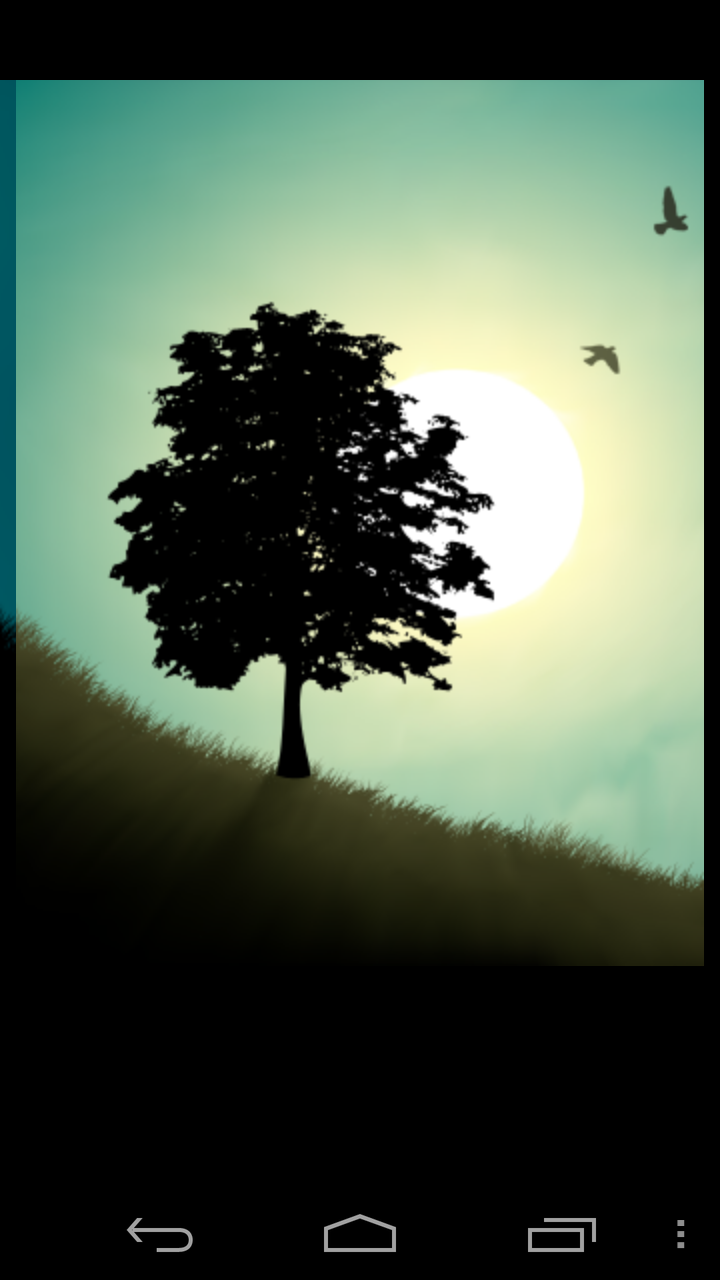
\includegraphics[width=0.800\linewidth]{biozen_feedback.png}
\caption[BioZen feedback]{BioZen feedback consisting of a sun varying from dark (low alpha) to light (high alpha).
A new age soundtrack loops in the background (can be
disabled in the configuration).}\label{ch-background/index:fig-background-biozen-feedback}\end{subfigure}
\begin{subfigure}[t]{0.30\linewidth}
\centering
\capstart

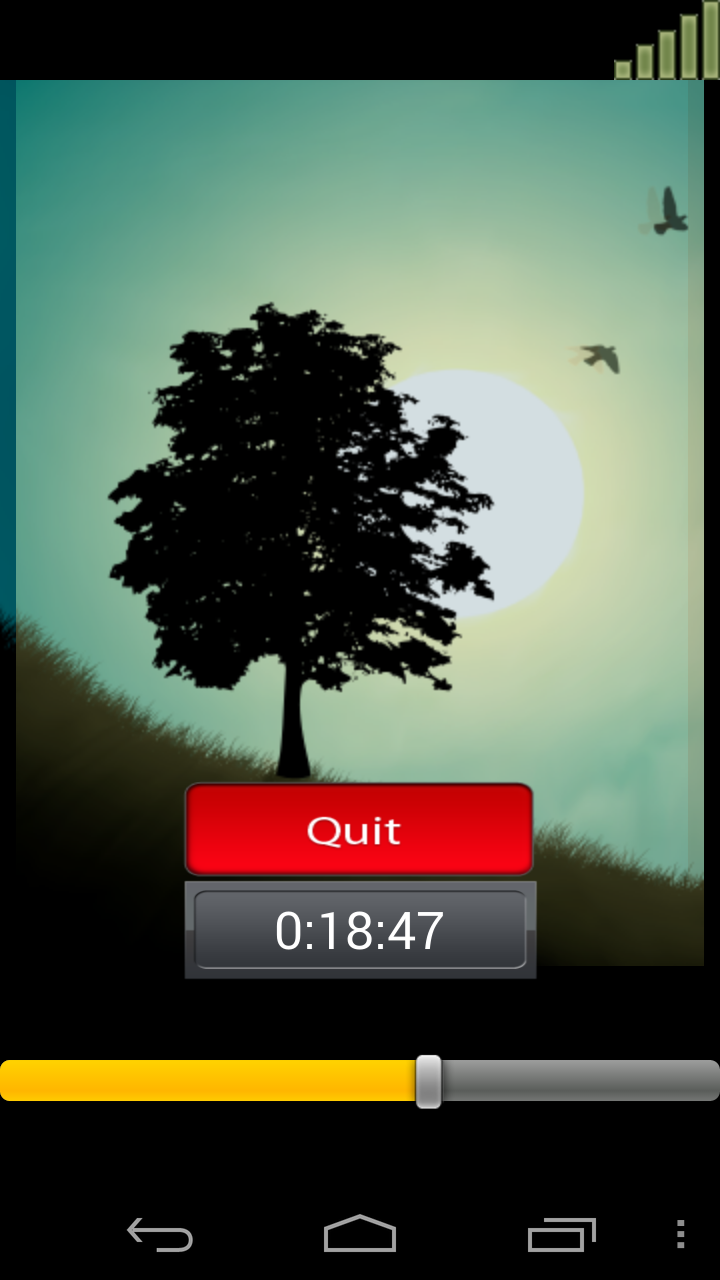
\includegraphics[width=0.800\linewidth]{biozen_feedback_gain_control.png}
\caption[Gain alpha.]{The input gain of the feedback parameter (i.e. the alpha band) can be adjusted through a slider thus providing a manual calibration.}\label{ch-background/index:fig-background-biozen-feedback-gain-control}\end{subfigure}
\begin{subfigure}[t]{0.30\linewidth}
\centering
\capstart

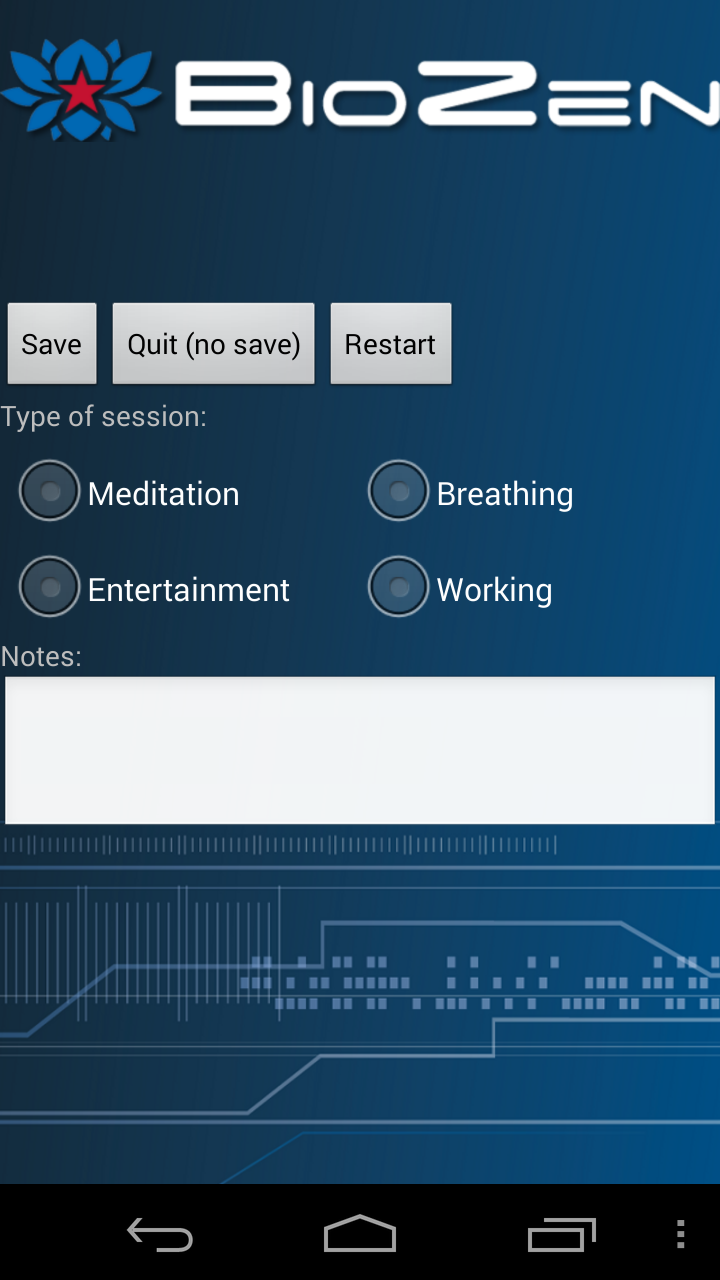
\includegraphics[width=0.800\linewidth]{biozen_feedback_save.png}
\caption[Save feedback session.]{Save feedback session with a tag (meditation, breathing, entertainment or
working) and a note.}\label{ch-background/index:fig-background-biozen-feedback-save}\end{subfigure}
\caption[Screen shoots of the neurofeedback from the BioZen Android app using the MindWave BCI]{Screenshots of the neurofeedback from the BioZen Android app using
the MindWave BCI (Images courtesy of BioZen).}\phantomsection\label{ch-background/index:fig-background-biozen-app-feedback}

\end{figure}


The feedback consists of an image of a hill in which the background brightness
and the visibility of a foreground tree are the feedback variables. The
background is brighter when the chosen parameter (e.g. some EEG power band) is
higher while the foreground tree is more visible when the chosen parameter is
more stable \cite{t2_biozenusersman_1_7_0.pdf_2013} (see Figure \ref{ch-background/index:fig-background-biozen-app-feedback}).


\subsection{Smartphone Brain Scanner 2}
\label{ch-background/index:smartphone-brain-scanner-2}\label{ch-background/index:ch-background-smartphone-brain-scanner-2}
The Smartphone Brain Scanner is developed at the Technical University of Denmark
(DTU). The project aims at moving EEG research out of the laboratory by means of
low cost wireless BCIs and smart phone based real-time neuroimaging software
which ``\emph{may transform neuroscience experimental paradigms}`` \cite{stopczynski_smartphones_2013}. The important notion here is that while
leaving the laboratory and using consumer interfaces, the focus is still on
research.

They are in principle headset agnostic and support the \emph{Easy Cap} and EPOC (described in Section {\hyperref[ch-background/index:ch-background-epoc]{2.2.1}})
BCIs. The EPOC is both used in its standard configuration and in a modified
configuration in which it is merged with hi-fi gel based electrodes. On the
software side, they use their Smartphone Brain Scanner (SBS2) open source
software framework including state of the art EEG signal processing such as
source reconstruction, noise filtering and frequency analysis \footnote{
: \href{https://github.com/SmartphoneBrainScanner}{https://github.com/SmartphoneBrainScanner}
}. It is build on the QT C++ framework \footnotemark[14] which allows compilation to the major desktop and
mobile operating systems. However, it is not trivial to embed a QT module inside
another native applications e.g. on the Android platform. Wireless connection to
the EPOC BCI goes via an USB dongle and requires an Android phone to be rooted
to function, the platform does not provide an easy way of interfacing with BCIs
via bluetooth. Furthermore it requires the research edition of the EPOC.

To validate the design of the Smartphone Brain Scanner, the research team behind
has build 3 brain imaging applications including an alpha training
application. Again, the focus is on research - specifically, the interface
parameters of neurofeedback training are investigated. The efficacy of two
different feedbacks were compared in a controlled study by measuring increase in
alpha amplitudes with each interface during a week of intensive training. One
feedback show a square changing colors between blue over gray to red for which
red represents high alpha. In another interface, high alpha amplitudes manifests
itself in the creation of small boxes and the color of the boxes created. By
keeping the created boxes visible during the 5 minute training period, the
interface reveals performance history thus ``\emph{allowing the user to easily compare
methods for increasing the amplitudes}`` \cite{stopczynski_smartphones_2013} (Figure \ref{ch-background/index:fig-related-smartphone-brain-scanner-feedback}). The training effect
measured by comparing baselines revealed only a statistic significant increase
in alpha for the box changing colors while the alpha levels during training were
significantly higher using the square creation interface.

The conclusions especially relevant to this thesis are that:
\begin{enumerate}
\item {} 
Alpha feedback training is feasible in a mobile setup.

\item {} 
Alpha levels during training (effect of feedback) is not necessarily
correlated with a general increase in alpha levels (effect of training).

\end{enumerate}
\begin{figure}[tbp]
\centering
\capstart

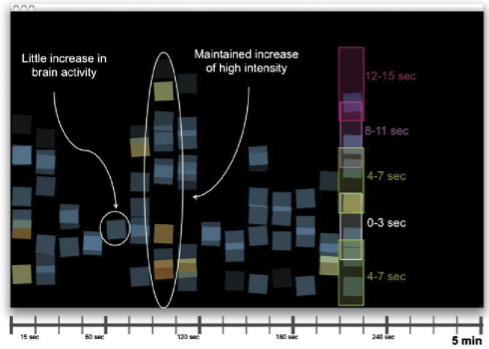
\includegraphics[width=0.600\linewidth]{smartphone-brain-scanner-feedback.png}
\caption[Smartphone Brain Scanner neurofeedback interface]{Smartphone Brain Scanner neurofeedback interface. High alpha amplitudes manifests
itself in the creation of small boxes and their color. By
keeping the created boxes visible during the 5 minute training period, the
interface reveals performance history \cite{stopczynski_smartphones_2013}.
Image courtesy of the Smartphone Brain Scanner project.}\label{ch-background/index:fig-related-smartphone-brain-scanner-feedback}\end{figure}


\section{Sum up of background and related systems}
\label{ch-background/index:sum-up-of-background-and-related-systems}
Table \ref{ch-background/index:table-related-systems} lists neurofeedback systems
which are either commercially available or use a consumer BCI.
These systems have been chosen because they
outline the current state of systems in the domain of AlphaTrainer.
The parameters highlighted in the table express
parameters desirable or necessary for a consumer neurofeedback system.
No existing system includes all parameters. For example,
no consumer available system includes the ability to give feedback on individually
adapted frequency bands which is important for the effectiveness of
the feedback training (see Section {\hyperref[ch-background/index:sec-background-stress-alpha-feedback-training]{2.3.2}}).
This ``gap'' among current neurofeedback systems is our motivation
for designing and building
AlphaTrainer as discussed in the following chapters.


\begin{table}
\capstart
\begin{center}

\bodyspacing

\begin{tabular}{>{\raggedright\arraybackslash}p{0.20\linewidth} p{0.20\linewidth} p{0.10\linewidth} p{0.10\linewidth}  p{0.20\linewidth}}

\toprule
\textsf{\relax 
Parameters
} & \textsf{\relax 
Brainwave Visualizer \&
Transcend
} & \textsf{\relax 
Brianball
} & \textsf{\relax 
BioZen
} & \textsf{\relax 
Alpha feedback app -
Smartphone Brain Scanner
}\\
\hline\midrule

\textbf{Convenient (dry sensor +
bluetooth connectivity)}.
 & 
yes
 & 
no
 & 
yes
 & 
no
\\

\textbf{Headset agnostic}.
 & 
no
 & 
no
 & 
yes
 & 
(yes)
\\

\textbf{Individual feedback.
spectra}
 & 
no
 & 
n/a
 & 
no
 & 
yes
\\

\textbf{Efficacy documented}.
 & 
no
 & 
no
 & 
no
 & 
yes
\\

\textbf{Available to customers}.
 & 
yes
 & 
yes
 & 
yes
 & 
no
\\

\textbf{Low cost}.
 & 
yes
 & 
no
 & 
yes
 & 
n/a
\\
\hline\bottomrule

\end{tabular}
\caption[Related systems]{Related systems}\phantomsection\label{ch-background/index:table-related-systems}
\end{center}
\end{table}


\chapter{Evaluation of 3 consumer BCIs}
\label{ch-experiment/index:ch-experiment}\label{ch-experiment/index::doc}\label{ch-experiment/index:evaluation-of-3-consumer-bcis}
This chapter addresses \textbf{G1} (Section {\hyperref[ch-intro/index:ch-intro-hypothesis-goals]{1.2}})
by evaluating 3 of the consumer BCIs presented in the Background Chapter {\hyperref[ch-background/index:ch-background]{2}}: EPOC (Section {\hyperref[ch-background/index:ch-background-epoc]{2.2.1}}), MindWave (Section {\hyperref[ch-background/index:ch-background-mindwave]{2.2.2}}) and TrueSense Kit (Section {\hyperref[ch-background/index:ch-background-truesense-kit]{2.2.3}}).  The BCIs are evaluated based on their
feasibility for alpha feedback training and finally in the conclusion of this
chapter we will select a BCI to use in the further development of
AlphaTrainer. This conclusion will be based on several aspects such as comfort
and connectivity. However, the main effort of this chapter is put into answering
the least accessible - and arguably the most important - factor: ``\emph{are the
BCIs able to measure alpha waves}''?

In designing an experiment to answer this, we did a
pre-study which is explained in the next section. After that we move on to
explain the setup, execution and data analysis of the actual experiment.

\textbf{Method}

To answer whether a BCI can measure alpha, we exploit the property of alpha
activity, that it is generally higher when eyes are closed compared to when eyes
are open \cite{bazanova_comments_2012}.  By comparing alpha levels
recorded under a closed-eyes condition to alpha levels recorded under an
open-eyes condition, we get a measure of how able a BCI is to detect alpha
activity.


\section{Pre-study}
\label{ch-experiment/index:pre-study}\label{ch-experiment/index:ch-experiment-pre-study}
The first BCI we got our hands on was the MindWave. Eager to find out
whether it could measure alpha levels, we implemented a simple proof-of-concept
prototype (explained in more detail in Chapter {\hyperref[ch-design/index:ch-design]{4}}) able
to store SDK alpha values (high and low alpha bands) as well as the
raw EEG signal. To get an initial idea whether the headset could measure
alpha, we used this prototype to record and compare SDK alpha values under
closed and open-eyes condition. Concretely, we performed some recordings
in which a test subject would have open eyes the first half and closed
eyes the last half of the recording. Figure \ref{ch-experiment/index:fig-mindwave-sdk-values}
shows two plots of SDK values recorded in this way - the plot on the right
has a y-axis limit while the plot on the left
shows the actual values.

\begin{figure}
\centering
\capstart
\begin{subfigure}[t]{0.48\linewidth}
\centering
\capstart

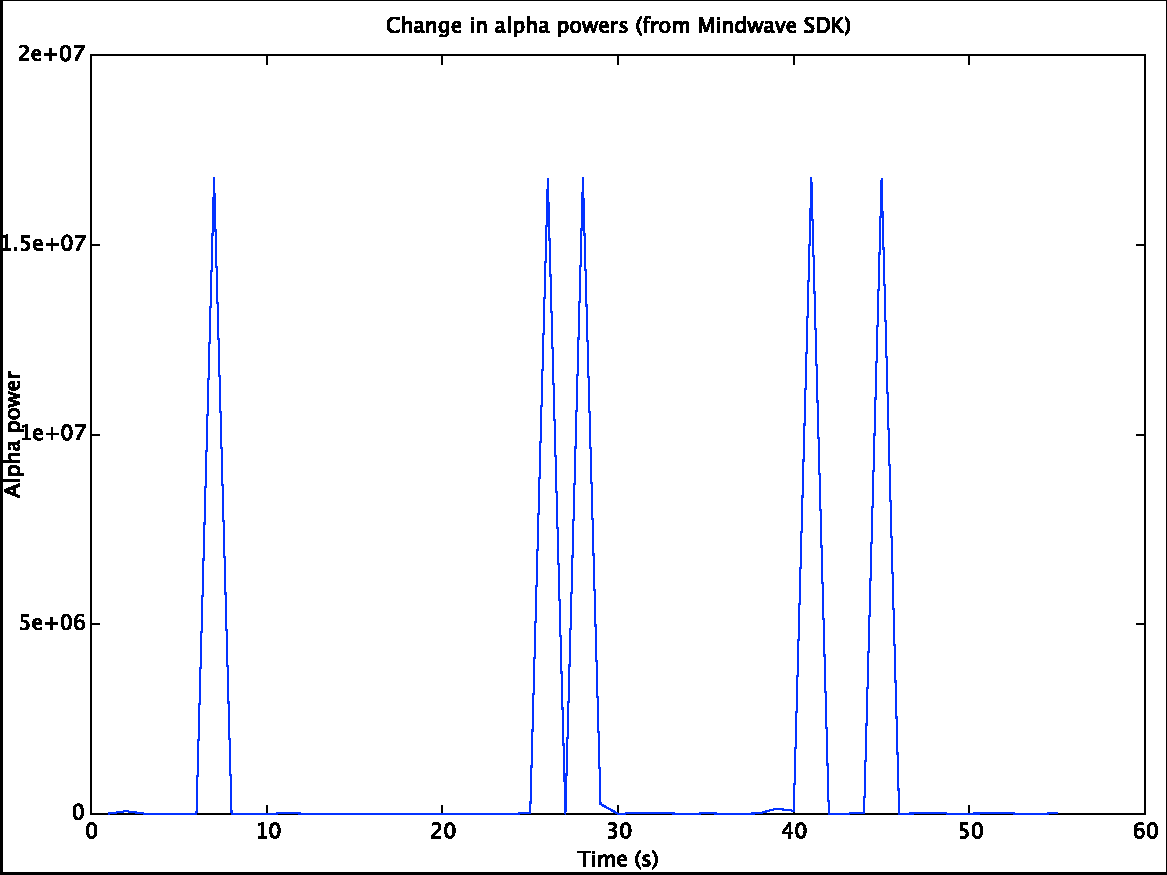
\includegraphics[width=1.000\linewidth]{mindwave_sdk_low_alpha_power.pdf}
\caption[No y-axis zoom]{No y-axis zoom.}\label{ch-experiment/index:fig-mindwave-sdk-low-alpha-power}\end{subfigure}
\begin{subfigure}[t]{0.48\linewidth}
\centering
\capstart

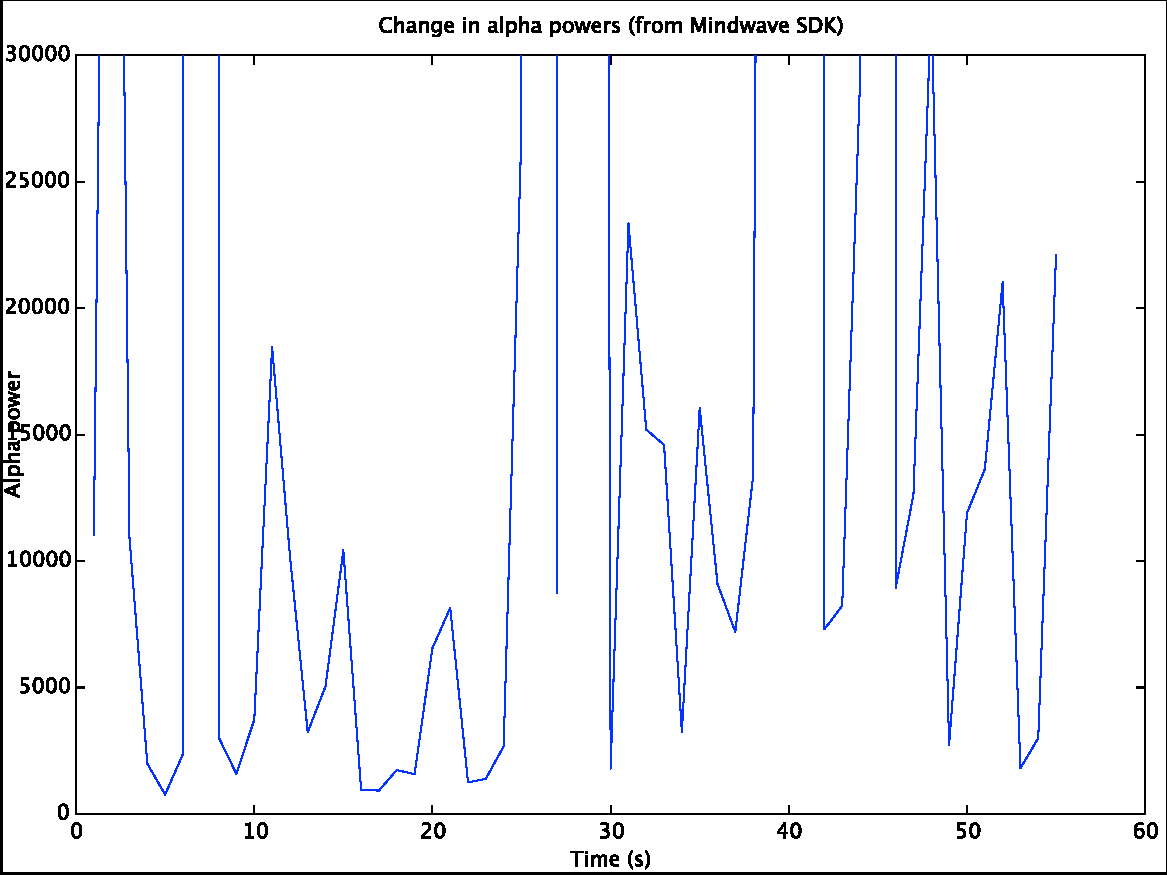
\includegraphics[width=1.000\linewidth]{mindwave_sdk_low_alpha_power_y_lim_30000.pdf}
\caption[With y-axis zoom (0 - 30,000)]{With y-axis zoom (0 - 30,000).}\label{ch-experiment/index:fig-mindwave-sdk-y-lim-30000}\end{subfigure}
\caption[Two plots of the same MindWave SDK alpha powers with/without zoom]{Two plots of the same MindWave SDK alpha powers with/without zoom.}\phantomsection\label{ch-experiment/index:fig-mindwave-sdk-values}

\end{figure}


The plot is representative for many similar recordings we performed and show some giant
outliers in the SDK values. Similar outliers were present in the other power
bands as well. To find out whether the outliers originated from the raw data or
the SDK data processing, we applied offline frequency analysis to the raw data
in Octave \footnote{
\href{http://www.gnu.org/software/octave}{http://www.gnu.org/software/octave}
} - an open-source equivalent to
MATLAB.  We were not able to reproduce the outliers which means they were not
present in the raw data. We initiated a correspondence with NeuroSky technicians
(see Appendix {\hyperref[appendix_experiment_mindwave_fora_posts:appendix-experiment-mindwave-fora-posts]{\emph{MindWave forum posts}}}) but they
were unable to pinpoint the origin of the outliers in spite of receiving both
SDK values and the originating raw data. They were also unable to disclose how
the SDK values are calculated due to the closed source nature of their SDK.

In the process of investigating the origin of the outliers, we also suspected
EMG and EOG noise. This led us to compare recordings in which we induced such
noise to recordings where we minimized it as much as possible by relaxing facial
muscles and avoiding eye movement.  While this did not prevent the outliers, it
showed a significant impact of the noise in the form of a general increase in band power
across all frequency bands. This led us to the insight that we would need to
minimize facial muscles and eye movement in the actual experiment as much as
possible.

From this point, we cleaned the MindWave SDK data by replacing the outliers with
the mean value of the non-outliers. We carried on the recordings to compare the
alpha levels when eyes are open to when they are closed. A representative plot
of the resulting data can be seen in Figure \ref{ch-experiment/index:fig-early-open-closed-experiments}.  In this case we recorded for 4
minutes and summed the alpha levels in bins of 2 seconds. As exemplified in the
plot, we measured a clear tendency of an increase in alpha when the test subject
closed the eyes at the midpoint of the recording.

\begin{figure}
\centering
\capstart
\begin{subfigure}[t]{0.48\linewidth}
\centering
\capstart

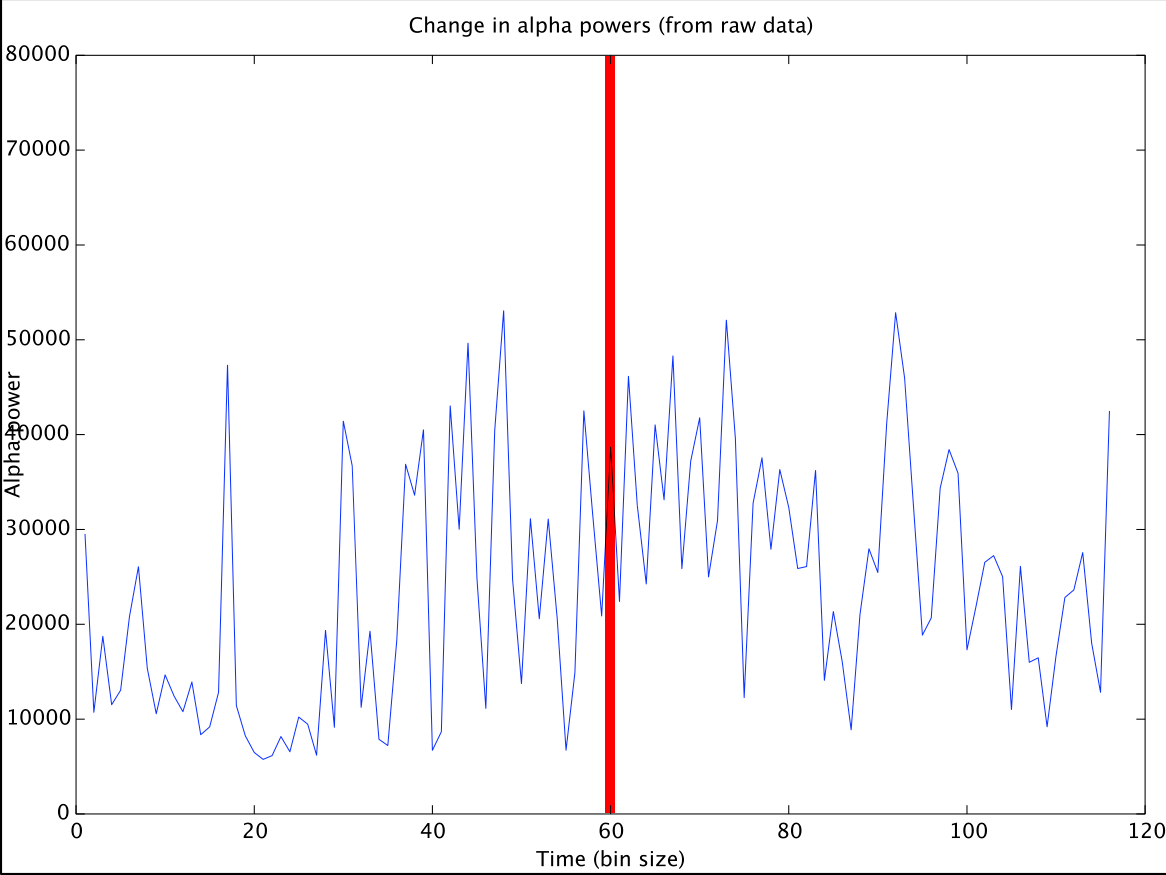
\includegraphics[width=1.000\linewidth]{alpha-bin-2s-raw-eeg.png}
\caption[Alpha powers (from raw data)]{Alpha powers (from raw data).}\label{ch-experiment/index:fig-experiment-alpha-bin-2s-raw-eeg}\end{subfigure}
\begin{subfigure}[t]{0.48\linewidth}
\centering
\capstart

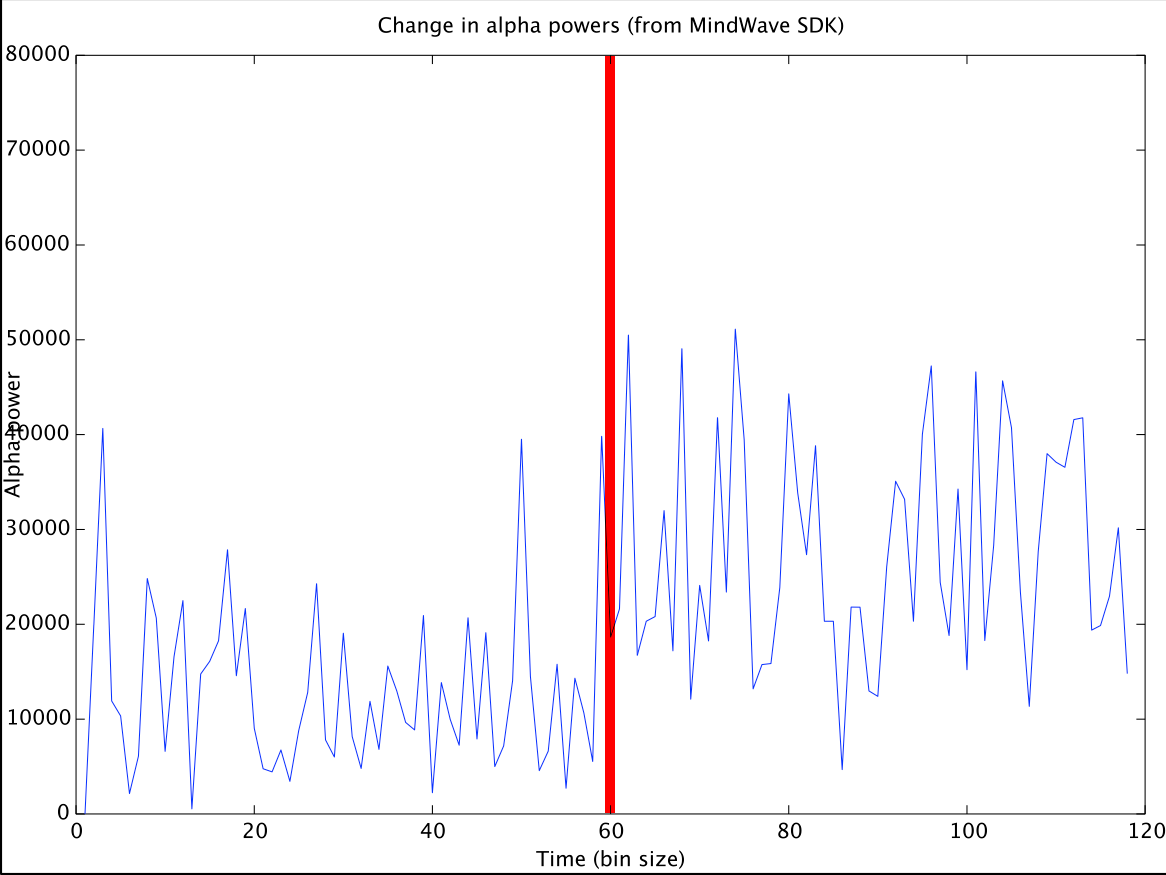
\includegraphics[width=1.000\linewidth]{alpha-bin-2s-sdk.png}
\caption[Alpha powers (from MindWave SDK)]{Alpha powers (from MindWave SDK, outliers removed).}\label{ch-experiment/index:fig-experiment-alpha-bin-2s-sdk}\end{subfigure}
\caption[Alpha levels recorded with open eyes (first half) and closed eyes (second half)]{Alpha levels recorded with open eyes (first half) and closed eyes (second half).}\phantomsection\label{ch-experiment/index:fig-early-open-closed-experiments}

\end{figure}


To avoid dependencies on black box SDK calculations and to get comparable
results across different BCIs, we chose to rely only on our own signal
processing from this point.  Both the TrueSense Kit and the EPOC (research
edition) BCIs support raw EEG out of the box through their bundled software OPI
Console and TestBench (Appendix {\hyperref[appendix_background_truesense_console:appendix-background-truesense-console]{\emph{TrueSense Kit console}}} and Appendix {\hyperref[appendix_background_testbench:appendix-background-testbench]{\emph{Emotiv EPOC TestBench}}}).

Next step was to select which of the 16 electrode(s) to use from the EPOC
headset. We chose to use one of the electrodes placed at location O1 or O2 (back
of the head) - the electrodes used in the Smartphone Brain Scanner alpha
feedback training application \cite{stopczynski_smartphones_2013}. This placement has the advantage of
little EOG and EMG noise (which we tested by comparing recordings from different
electrodes while introducing eye movement and facial muscle activation). We did
not experience significant difference between the two channels and we decided to
use only the O1 electrode in order to make sure results could be directly
compared to the results of the other single channel BCIs.

Furthermore we had to decide the placement of the TrueSense Kit BCI. It features
flexible mounting by its small size and elastic band mount, so placement is not
obvious. To obtain the advantages of recording from the back of the head, we
tried mounting the sensor on top of the neck hair at O1. This gave us very noisy
data both in the dry and the gel-pad electrode configuration probably due to low
scalp conductivity. The same was the case when trying to place the sensor on the
temple. We ended up placing the sensor at the side of the forehead as
recommended by TrueSense Kit for measuring alpha \footnote{
\href{http://op-innovations.com/en/wearsensor}{http://op-innovations.com/en/wearsensor}
}. Finally, we decided to record the TrueSense
Kit over radio (ZigBee) rather than to the memory module attachable to the
sensor. The latter would presumably give better
recording quality. However, in a neurofeedback context offline
recording is not relevant since the data must be fed into the feedback
mechanism instantly.

This concludes the pre-study which incrementally has led to all the building
blocks necessary for designing an experiment which will answer whether the BCIs
of interest can measure alpha.


\section{Experiment design}
\label{ch-experiment/index:experiment-design}
This section formalizes the design of our experiment which will
answer to which degree the BCIs can measure alpha from guidelines
by MacKenzie \cite{mackenzie_human-computer_2013}.
Revisiting our
method, it is assumed that alpha levels are higher when eyes are
closed than when eyes are open. From this assumption, we reach
the hypothesis tested in the experiment:

H1
\begin{quote}

The EEG recorded while eyes are closed contains higher alpha levels
than EEG recorded while eyes are open.
\end{quote}

The independent variables (factors) of the experiment are the \emph{eye states}:
(\emph{i}) open; and (\emph{ii}) closed. The dependent variable is simply the alpha
level. The task of the participants is to relax as much as possible (keep
blink, face muscles and eye-movement at a minimum). We did a pilot experiment on
our selves and on a domain expert within experimental psychology to catch
potential problems which led to a slight refining of the execution procedure.
We later carried out the experiment on 6 participants (4 males and 2 females).

To ensure that we would not only measure a precedence effect or some other
learning effect - i.e. gaining familiarity with wearing a brain interface and
thus being increasingly comfortable and relaxed (which minimizes EMG and EOG
noise) - we varied the BCI recording order as lined out in Table \ref{ch-experiment/index:table-experiment-headset-latin-square}. We now describe in more detail
the execution of the experiment.


\begin{table}
\capstart
\begin{center}

\begin{tabular}{r l l l}

\toprule
\textsf{\relax 
Participant
} & \textsf{\relax 
Headset 1
} & \textsf{\relax 
Headset 2
} & \textsf{\relax 
Headset 3
}\\
\hline\midrule

1
 & 
EPOC (o/c)
 & 
MindWave (c/o)
 & 
TrueSense Kit (o/c)
\\

2
 & 
MindWave (c/o)
 & 
TrueSense Kit (o/c)
 & 
EPOC (c/o)
\\

3
 & 
TrueSense Kit (o/c)
 & 
EPOC (c/o)
 & 
MindWave (o/c)
\\

4
 & 
TrueSense Kit (c/o)
 & 
MindWave (o/c)
 & 
EPOC (c/o)
\\

5
 & 
EPOC (o/c)
 & 
TrueSense Kit (c/o)
 & 
MindWave (o/c)
\\

6
 & 
MindWave (c/o)
 & 
EPOC (o/c)
 & 
TrueSense Kit (c/o)
\\
\hline\bottomrule

\end{tabular}
\caption[Experiment order for headsets and participants]{Experiment order for headsets and participants - o = open and c = closed}\phantomsection\label{ch-experiment/index:table-experiment-headset-latin-square}
\end{center}
\end{table}


\subsection{Execution}
\label{ch-experiment/index:table-experiment-headset-latin-square}\label{ch-experiment/index:execution}
The setting was a dark room with no sun light, a lap top computer with
a still image to focus on (Hokusai, ``The great wave''), a table and an office
chair (Figure \ref{ch-experiment/index:fig-experiment-setup}).

\begin{figure}
\centering
\capstart
\begin{subfigure}[t]{0.35\linewidth}
\centering
\capstart

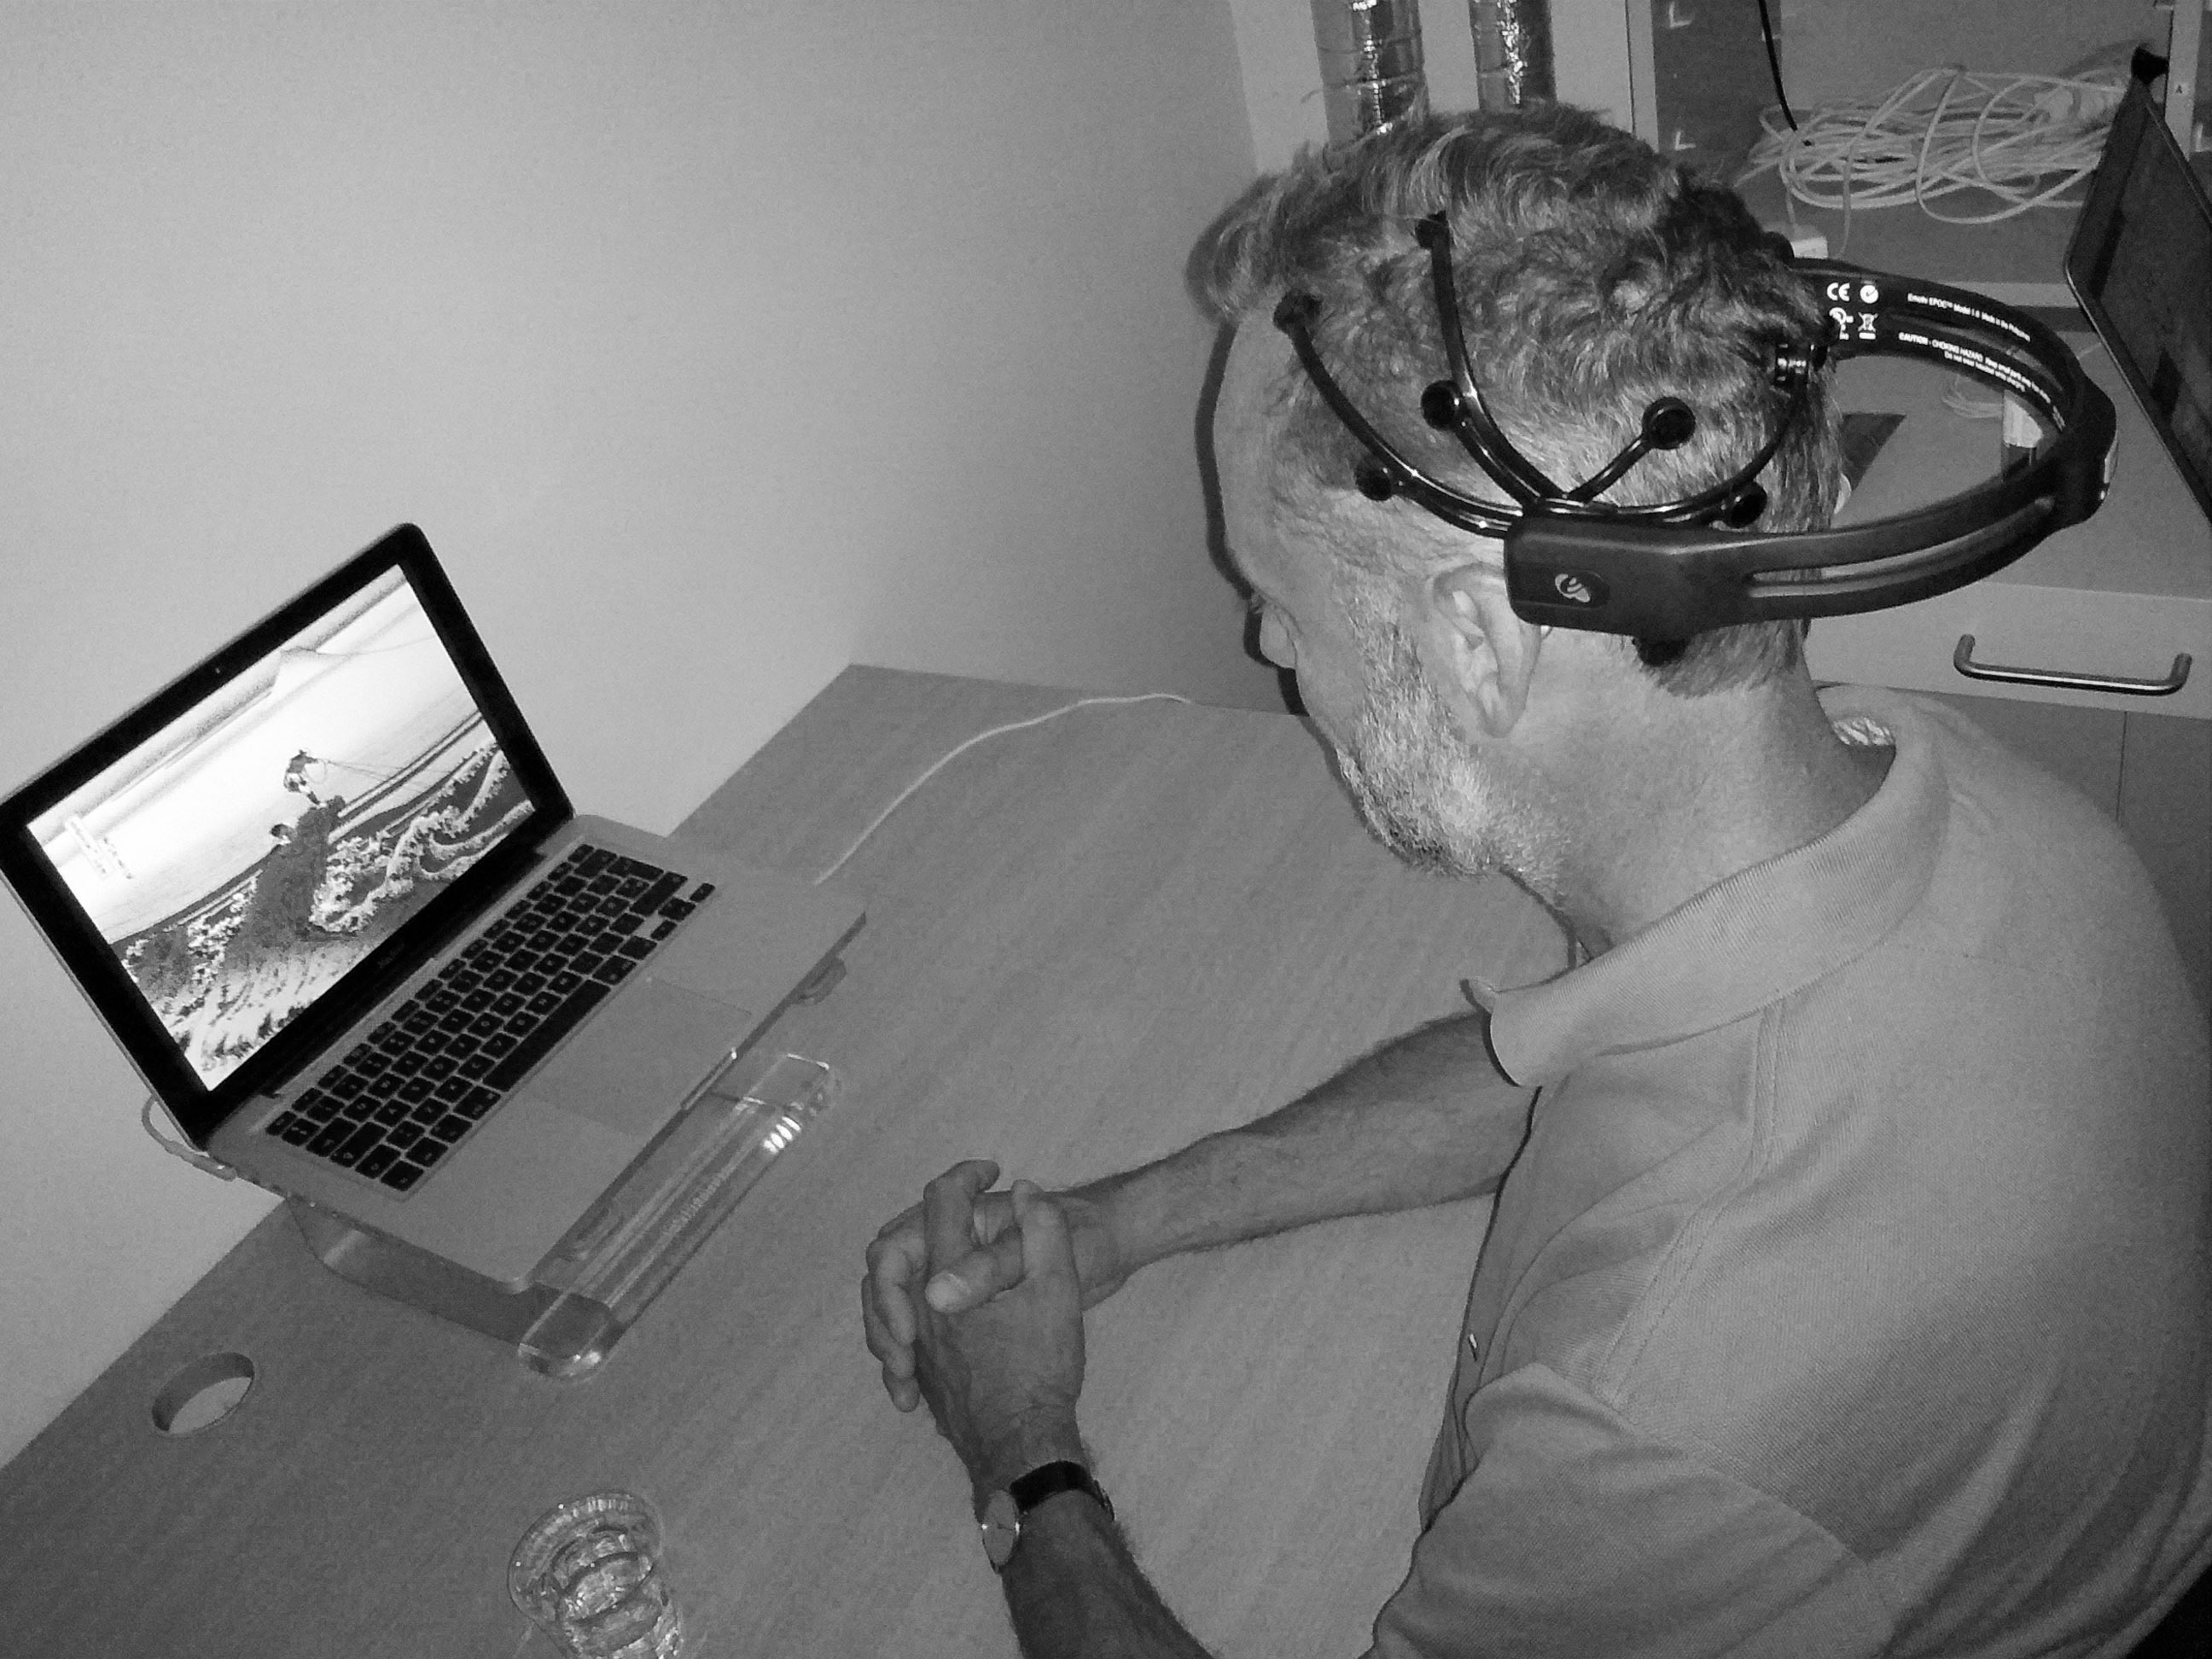
\includegraphics[width=1.000\linewidth]{experiment-setup-w-epoc.jpg}
\caption[Using EPOC]{Using EPOC.}\label{ch-experiment/index:fig-experiment-setup-w-epoc}\end{subfigure}
\begin{subfigure}[t]{0.35\linewidth}
\centering
\capstart

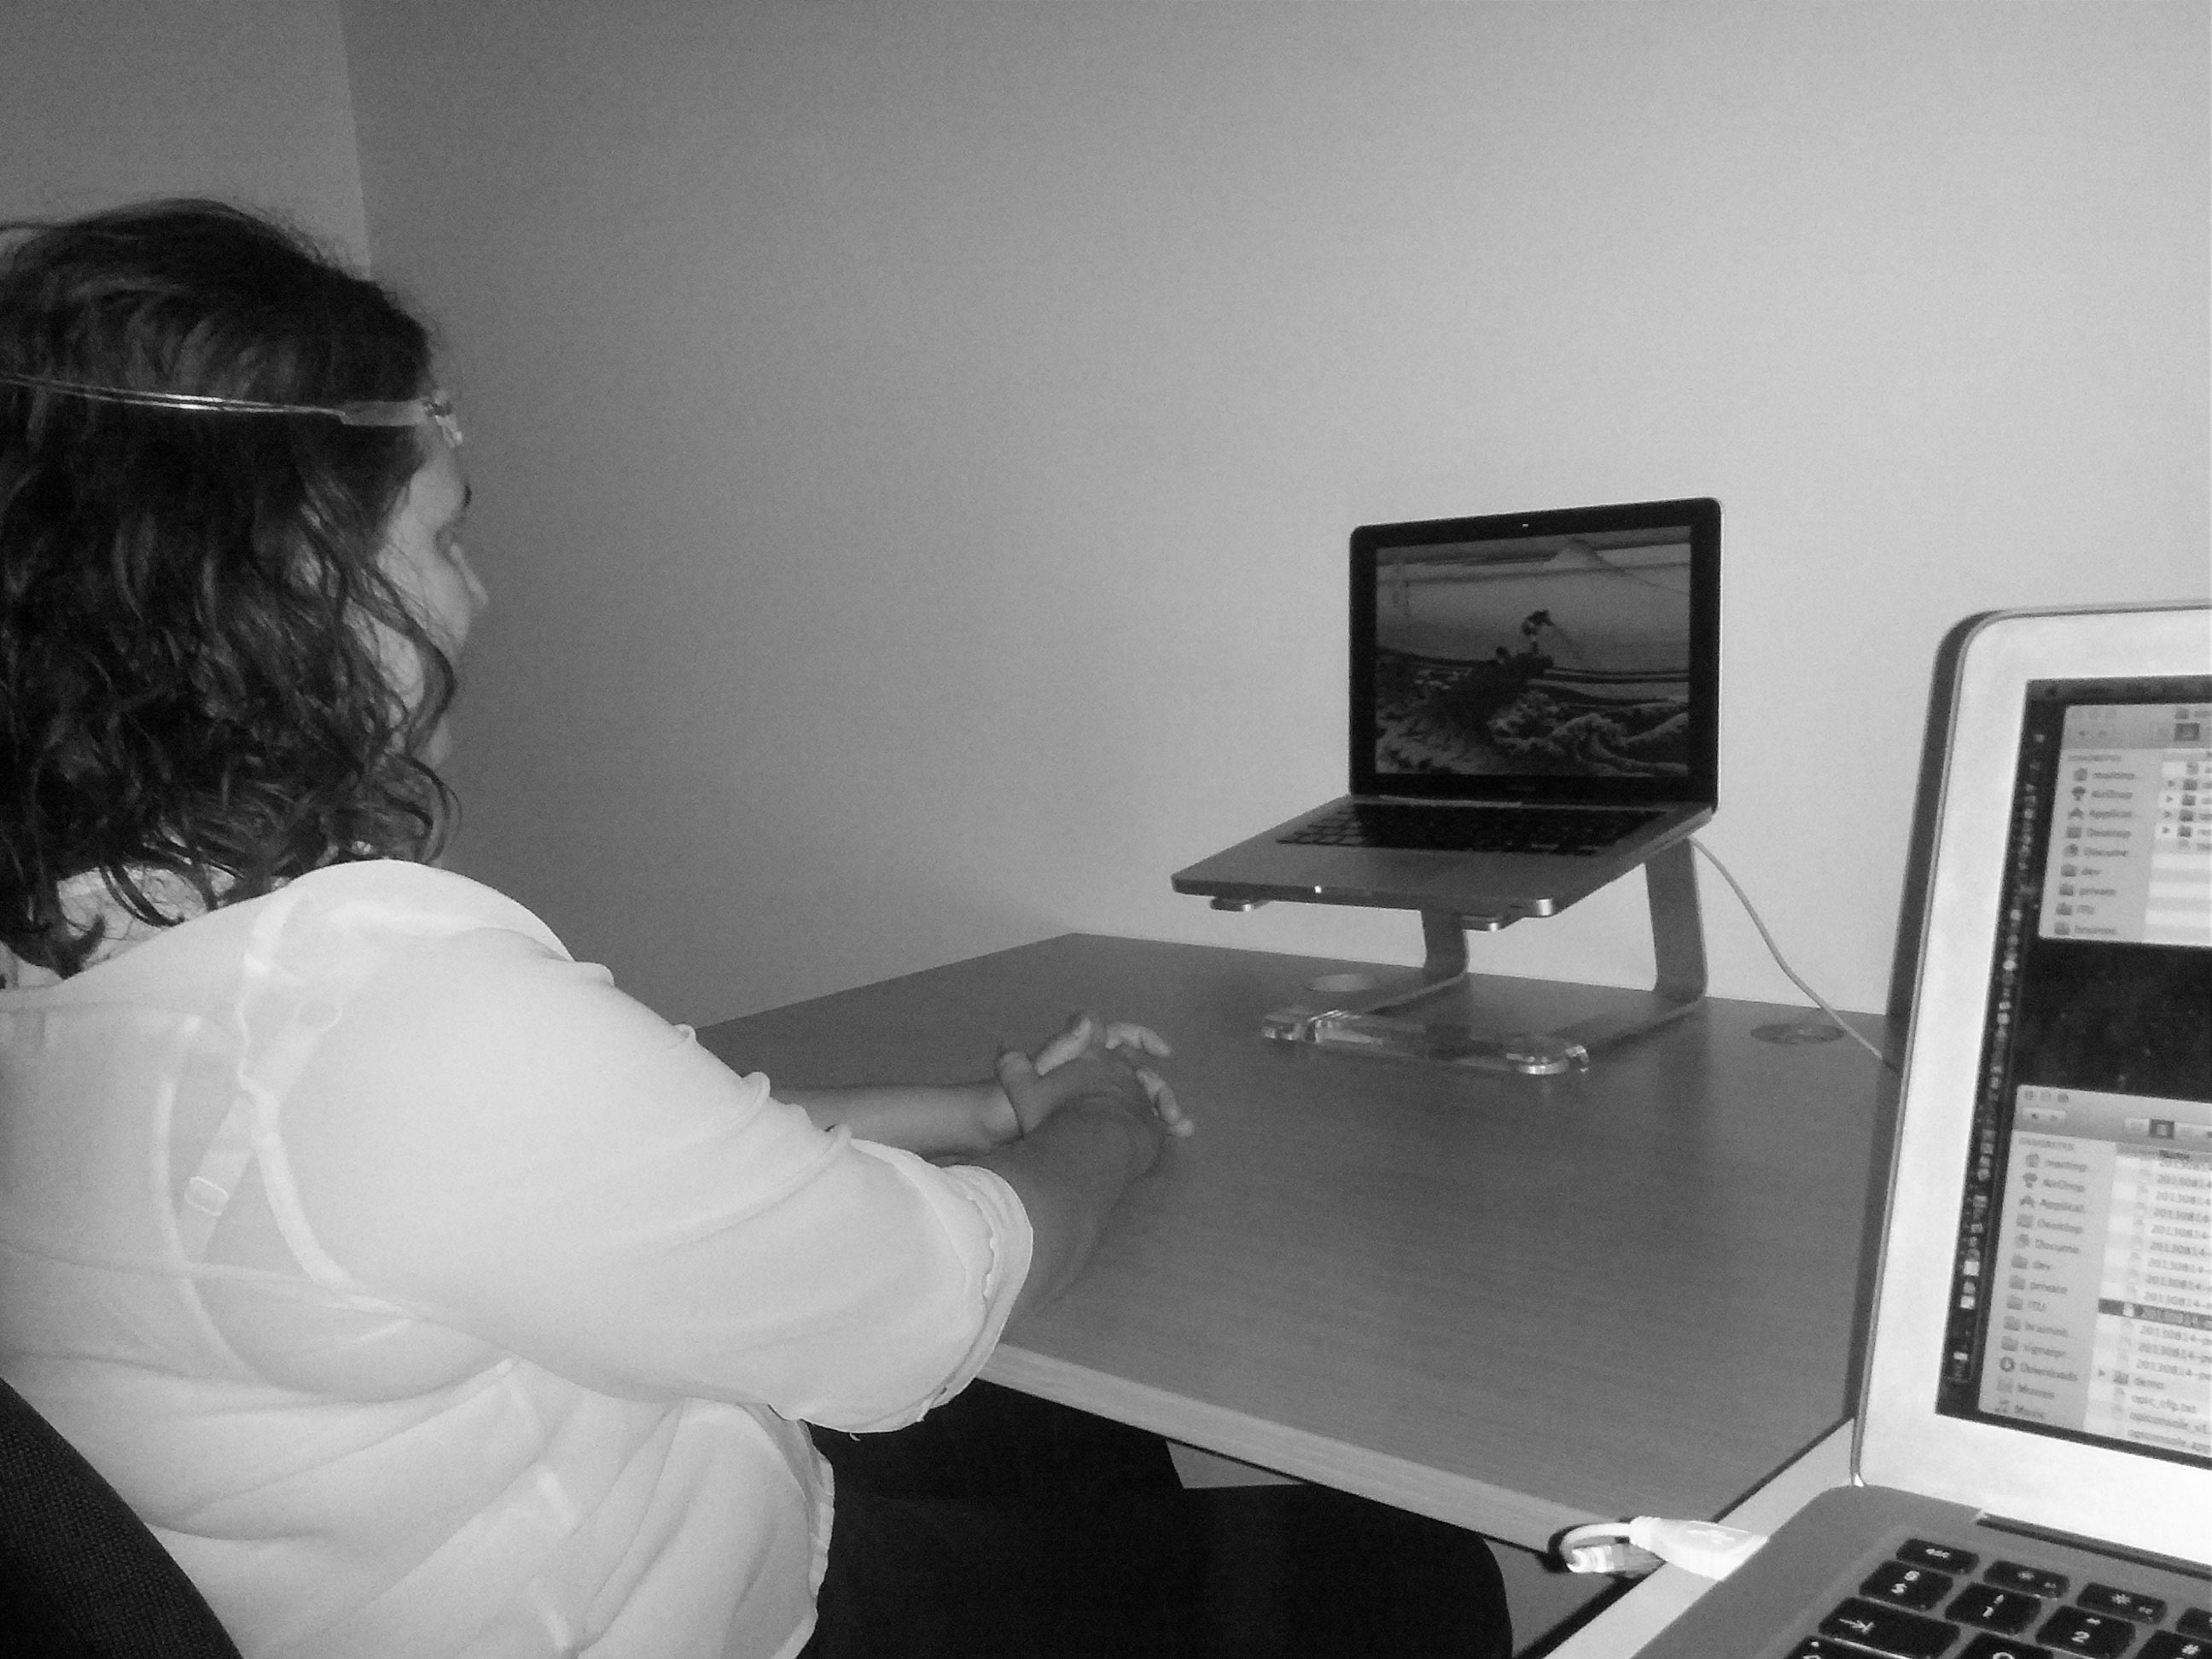
\includegraphics[width=1.000\linewidth]{experiment-setup-w-truesense.jpg}
\caption[Using TrueSense Kit]{Using TrueSense Kit.}\label{ch-experiment/index:fig-experiment-setup-w-sense}\end{subfigure}
\begin{subfigure}[t]{0.35\linewidth}
\centering
\capstart

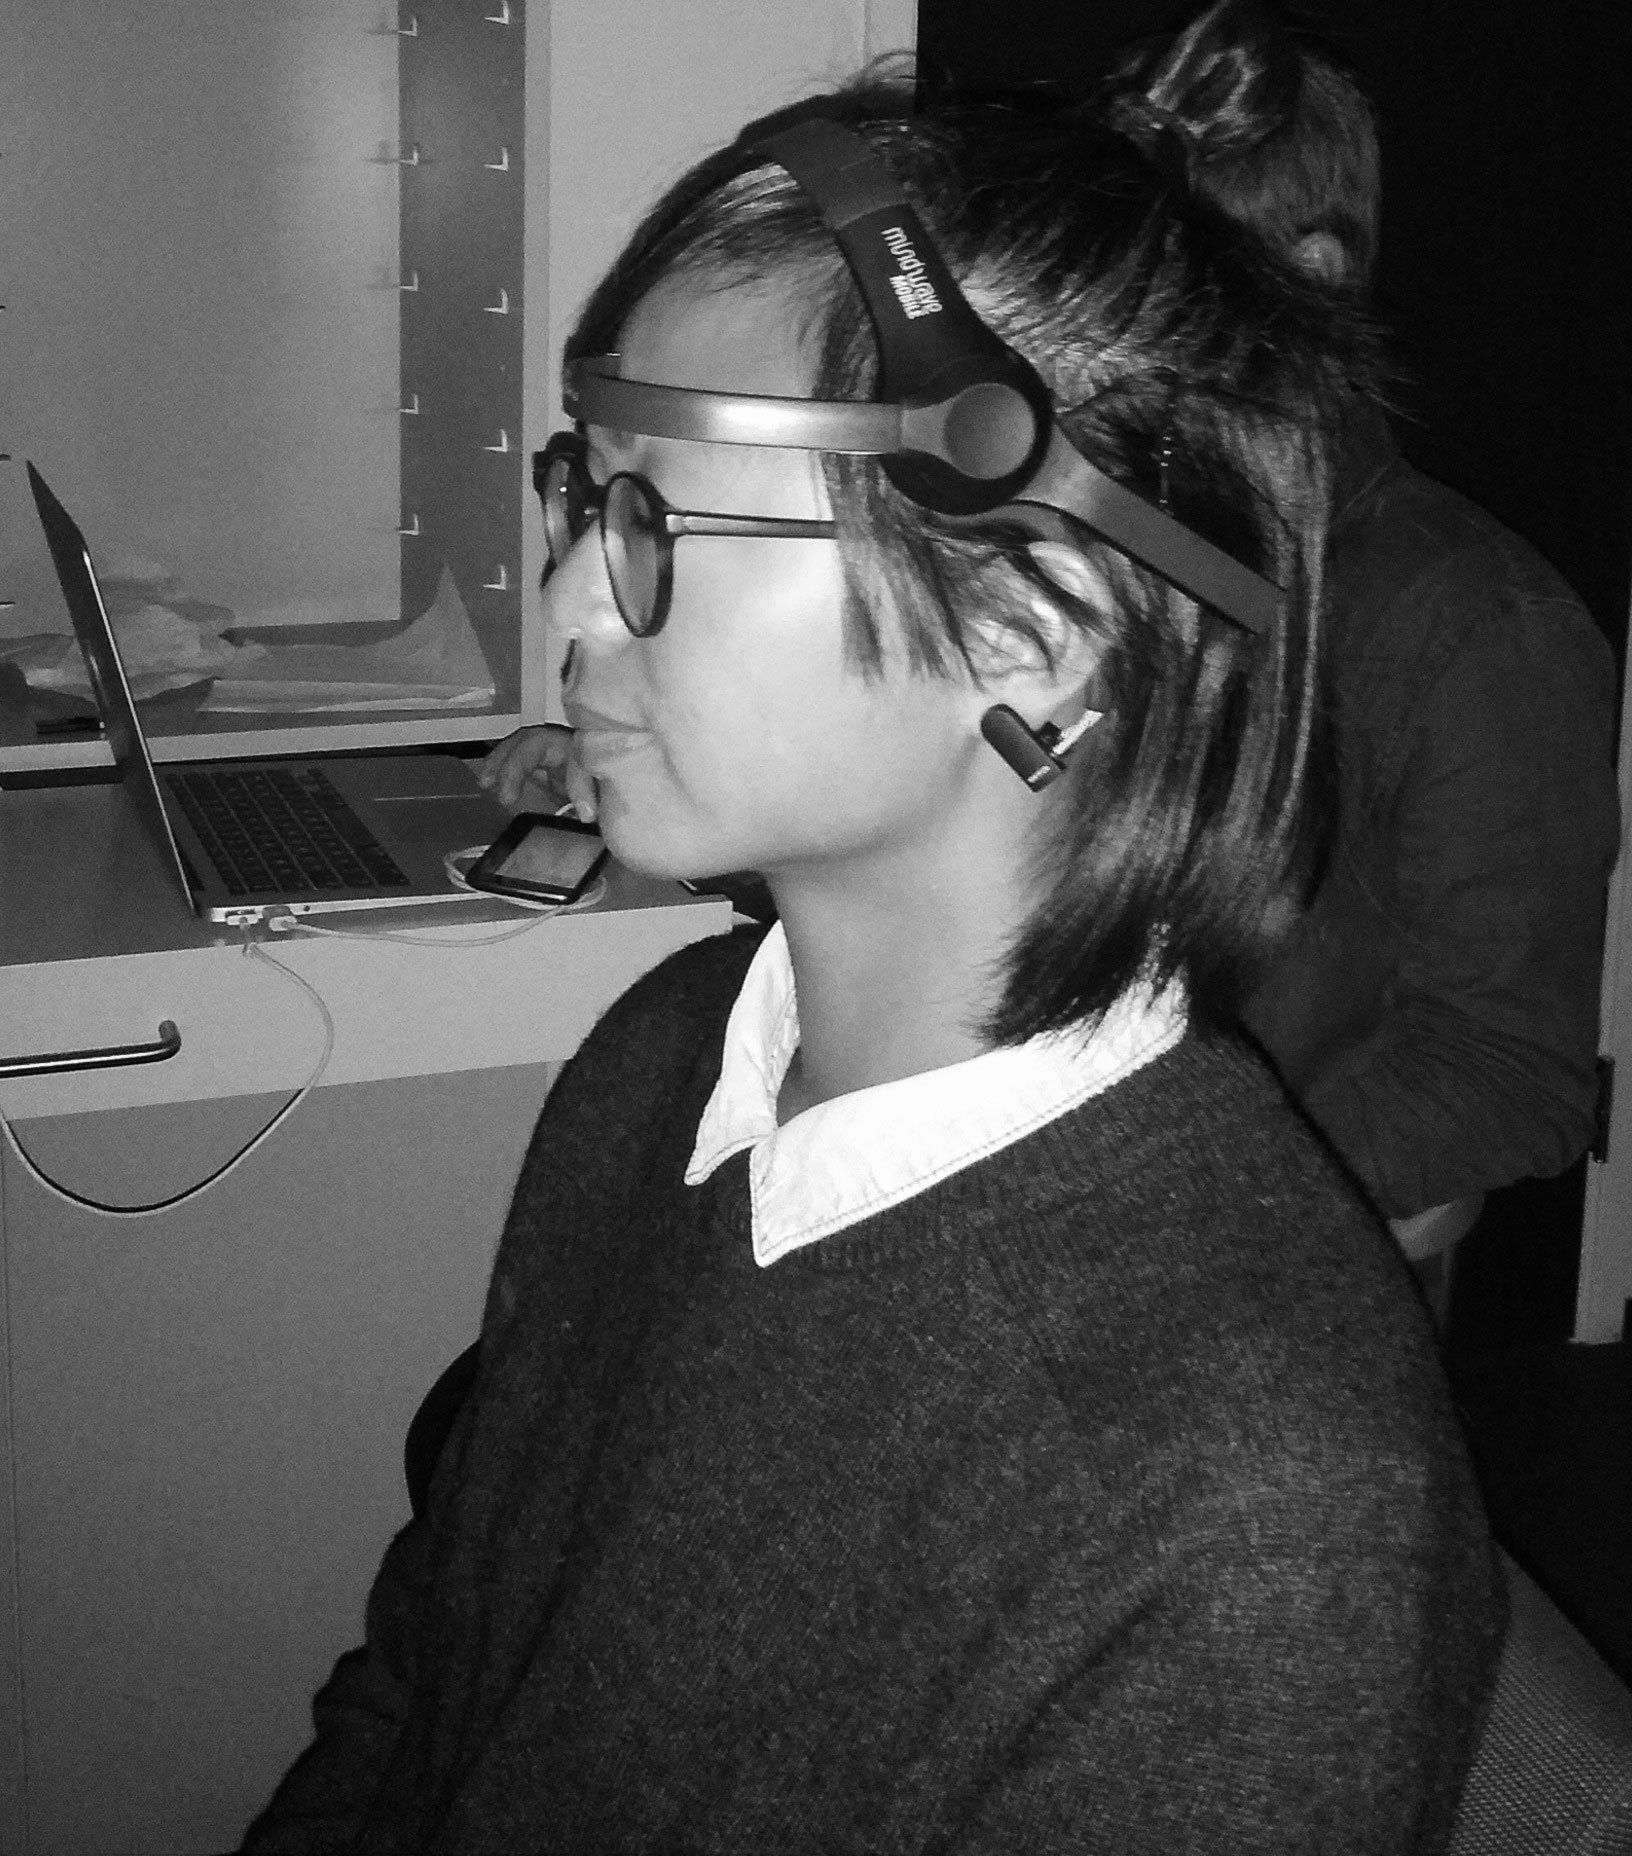
\includegraphics[width=0.700\linewidth]{experiment-setup-w-mindwave.jpg}
\caption[Using MindWave.]{Using MindWave.}\label{ch-experiment/index:fig-experiment-setup-w-mindwave}\end{subfigure}
\caption[Experiment setup]{Experiment setup.}\phantomsection\label{ch-experiment/index:fig-experiment-setup}

\end{figure}


Before entering the recording room, the participant was instructed in a
breathing exercise to help her relax. The exercise consisted of breathing slowly
through the nose while continuously counting 1 down when exhaling. The count
down starts from 4 and whenever 0 is reached it starts over from 4.

The procedure for each participant - BCI combination was this:
\begin{itemize}
\item {} 
The participant entered the recording room, sat down and got a headset mounted.

\item {} 
The participant was instructed to sit still, keep eye movement and
blinking to a minimum, relax face muscles and to do the simple
breathing exercise instructed earlier.

\item {} 
The participant was instructed to focus at a specific point in the image
when having open eyes (to hold visual stimuli constant across all participants and
headsets).

\item {} 
3 times in a row, we recorded for 5 minutes. After 2.5 minutes
the participant is instructed verbally to close or open her eyes.

\end{itemize}

This procedure was repeated until all 3 BCIs had been recorded.
After each session (3 recordings with the same headset) we asked
the participant: (\emph{i}) ``\emph{how relaxed did you feel during the recordings
from 1 to 10, where 10 is very relaxed?}''; and (\emph{ii}) ``\emph{how comfortable was
it to wear the headset from 1 to 10, where 10 is very comfortable?}''. The
results of this questionnaire are listed in Table \ref{ch-experiment/index:table-experiment-final-relaxed-comfort}. They indicate that
TrueSense Kit is the most comfortable BCI to wear and that the EPOC and
MindWave BCIs are both ``medium'' comfortable. The results also indicates
that the subjects were quite evenly relaxed across the different BCIs.


\begin{table}
\capstart
\begin{center}

\begin{tabular}{l l l l}

\toprule
\textsf{\relax } & \textsf{\relax 
EPOC
} & \textsf{\relax 
MindWave
} & \textsf{\relax 
TrueSense Kit
}\\
\hline\midrule

Level of relaxation
 & 
7.17 \(\pm\)1.60
 & 
8.17 \(\pm\)1.17
 & 
8.33 \(\pm\)0.82
\\

BCI comfort
 & 
5.67 \(\pm\)2.73
 & 
5.00 \(\pm\)1.67
 & 
8.50 \(\pm\)2.06
\\
\hline\bottomrule

\end{tabular}
\caption[Experiment micro questionary]{Experiment micro questionary}\phantomsection\label{ch-experiment/index:table-experiment-final-relaxed-comfort}
\end{center}
\end{table}


\subsection{Data processing, cleaning and analysis}
\label{ch-experiment/index:table-experiment-final-relaxed-comfort}\label{ch-experiment/index:ch-experiment-processing}\label{ch-experiment/index:data-processing-cleaning-and-analysis}
From the 5 minutes recorded, we extract 2 minutes of open eyes and 2 minutes of
closed eyes - thus discarding a 15 second margin on either side of each
extraction. These two extractions are subject for the frequency comparison.

For frequency estimation, we use the \emph{P.D. Welch algorithm} which cuts up the data
in small time windows and for each frequency in each window the density of that
frequency is calculated/estimated using FFT \cite{welch_use_1967}. These frequency densities are then squared and summed
up within a frequency band resulting in a total estimation of the power of that
frequency band in the input signal (Appendix {\hyperref[appendix_experiment:appendix-experiment]{\emph{Experiment - signal processing}}}).

We compare alpha levels between the open/closed eyes conditions in two ways:
(\emph{i}) Direct comparison by dividing alpha band power under closed-eyes condition
with alpha band power under open-eyes condition. This is how the alpha band
power is calculated in the Smartphone Brain Scanner alpha feedback training
experiment \cite{stopczynski_smartphones_2013}. We call this the
``\emph{absolute alpha}'' measure. (\emph{ii}) We also compare the relative alpha levels of
each condition. The relative alpha level is found by dividing the alpha band
power with a broad ``total'' band power (in our case 5 Hz - 25 Hz) to get a
measure of how much the total band power is made up of alpha. Dividing the
relative alpha level under closed-eyes condition with the relative alpha level
under open-eyes condition gives us the ``\emph{relative alpha}'' measure. This approach
is used in \cite{finnigan_resting_2011} to estimate theta band power.
\phantomsection\label{ch-experiment/index:equation-eq-absolute-alpha}\begin{gather}
\begin{split}\alpha_\textrm{absolute} = \frac{\sum \alpha_\textrm{closed eyes}} {\sum \alpha_\textrm{open eyes}}\end{split}\label{ch-experiment/index-eq-absolute-alpha}\\\begin{split}\end{split}\notag
\end{gather}\phantomsection\label{ch-experiment/index:equation-eq-relative-alpha}\begin{gather}
\begin{split}\alpha_\textrm{relative} = \frac{\dfrac{\sum \alpha_\textrm{closed eyes}}{\sum \textrm{ EEG power closed eyes} }}{\dfrac{\sum \alpha_\textrm{open eyes}}{ \sum \textrm{EEG power open eyes}}}\end{split}\label{ch-experiment/index-eq-relative-alpha}\\\begin{split}\end{split}\notag
\end{gather}
The absolute alpha measure compares the alpha levels under each condition
(open/closed eyes) isolated from the total EEG power level (Equation \eqref{ch-experiment/index-eq-absolute-alpha}). The relative alpha measure will account for the total
EEG power by comparing alpha relative to the total EEG power under each
condition (Equation \eqref{ch-experiment/index-eq-relative-alpha}). We expect the latter to be the most
reliable measure of alpha in that it will be more resistant to EMG/EOG noise
(under the assumption that such noise will raise the overall EEG power level
somewhat evenly which matches our observations from recordings under induced EMG
and EOG).

We did some simple filtering by discarding bins where the alpha or total band
power deviates from mean by more than 4 * std.dev.  In these cases, the power
would mainly origin from EMG/EOG. For each headset, this cleaning excluded 2 of
the 18 recordings.  The mean values \(\pm\) standard deviation are listed in Table \ref{ch-experiment/index:table-experiment-final-result-mean}. The mean value of the absolute
and relative alpha measures inform about the degree to which a higher alpha
level has been detected under closed-eyes condition.  The standard deviation
informs about the consistency of the recording measure and BCI combination
(lower std.dev. means more consistent).  The resulting data suggests:
\begin{itemize}
\item {} 
The EPOC and MindWave BCIs can detect alpha (mean is \textgreater{} 1).

\item {} 
The EPOC headset detect the most alpha.

\item {} 
The relative alpha measure is the most reliable (i.e. lower std.dev.) as
expected.

\item {} 
The TrueSense Kit sensor only shows a vague difference in alpha between the
two conditions which is unlikely to be
sufficient for alpha feedback training. Furthermore Figure \ref{ch-experiment/index:fig-experiment-final-7-truesense-alpha-power} exemplifies the general tendency that
the recordings of TrueSense Kit are noisy and lack the expected alpha peak
under closed-eyes condition. The narrow peak around 12,5 Hz is likely to be
some power grid noise being picked up (which we experienced a lot with the
TrueSense Kit). Figure \ref{ch-experiment/index:fig-experiment-final-13-truesense-alpha-power} also
show noisy data from the TrueSense Kit. In this case we see a lot of
low frequency noise and its harmonics - the series of peaks appearing approximately
every 3 Hz. This noise pattern is roughly the same under
open and closed eyes conditions which indicates that the main source of the
recording is not EEG (i.e. the alpha peak is missing).

\end{itemize}

Figure \ref{ch-experiment/index:fig-final-experiment-recording-7} and
Figure \ref{ch-experiment/index:fig-final-experiment-recording-13} show recordings of each
BCI for two different participants. They exemplify how the alpha peak varies
between individuals. For example, Participant 3 has an alpha peak under
closed-eyes condition around 10.5 Hz while participant 5 has one around 11.5 Hz.


\begin{table}
\capstart
\begin{center}

\begin{tabular}{r l l l}

\toprule
\textsf{\relax 
Measure
} & \textsf{\relax 
EPOC
} & \textsf{\relax 
MindWave
} & \textsf{\relax 
TrueSense Kit
}\\
\hline\midrule

Absolute alpha
 & 
4.50 \(\pm\)3.12
 & 
2.37 \(\pm\)1.54
 & 
0.87 \(\pm\)0.40
\\

Relative alpha
 & 
2.12 \(\pm\)0.63
 & 
1.55 \(\pm\)0.60
 & 
1.06 \(\pm\)0.21
\\
\hline\bottomrule

\end{tabular}
\caption[alpha measurement ability result]{Mean values of the absolute and relative alpha measures}\phantomsection\label{ch-experiment/index:table-experiment-final-result-mean}
\end{center}
\end{table}

\begin{figure}
\centering
\capstart
\begin{subfigure}[t]{0.49\linewidth}
\centering
\capstart

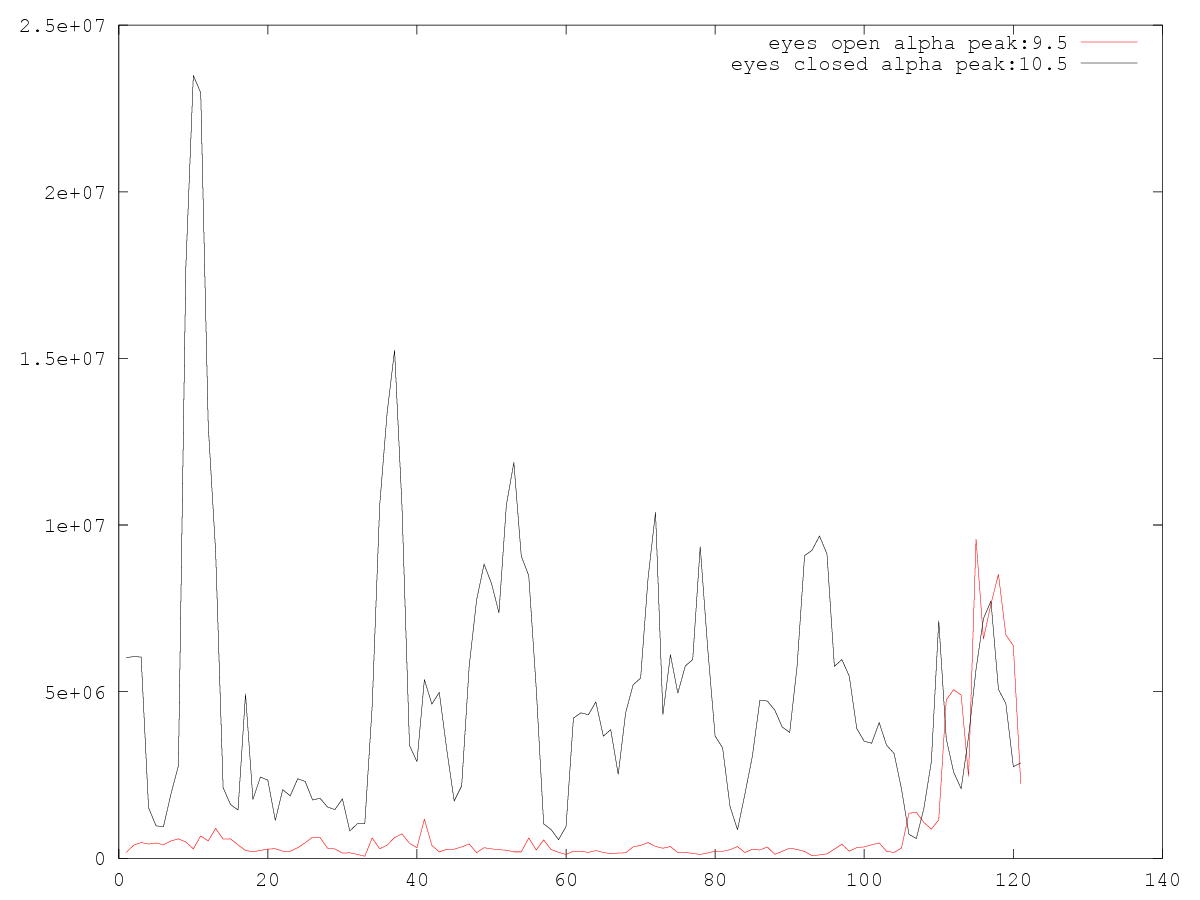
\includegraphics[width=1.000\linewidth]{experiment-final-7-epoc-alpha-progress.png}
\caption[EPOC alpha progress.]{EPOC alpha progress. Alpha peaks: 9,5 Hz (open eyes) and 10,5 Hz (closed eyes).}\label{ch-experiment/index:fig-experiment-final-7-emotiv-alpha-progress}\end{subfigure}
\begin{subfigure}[t]{0.49\linewidth}
\centering
\capstart

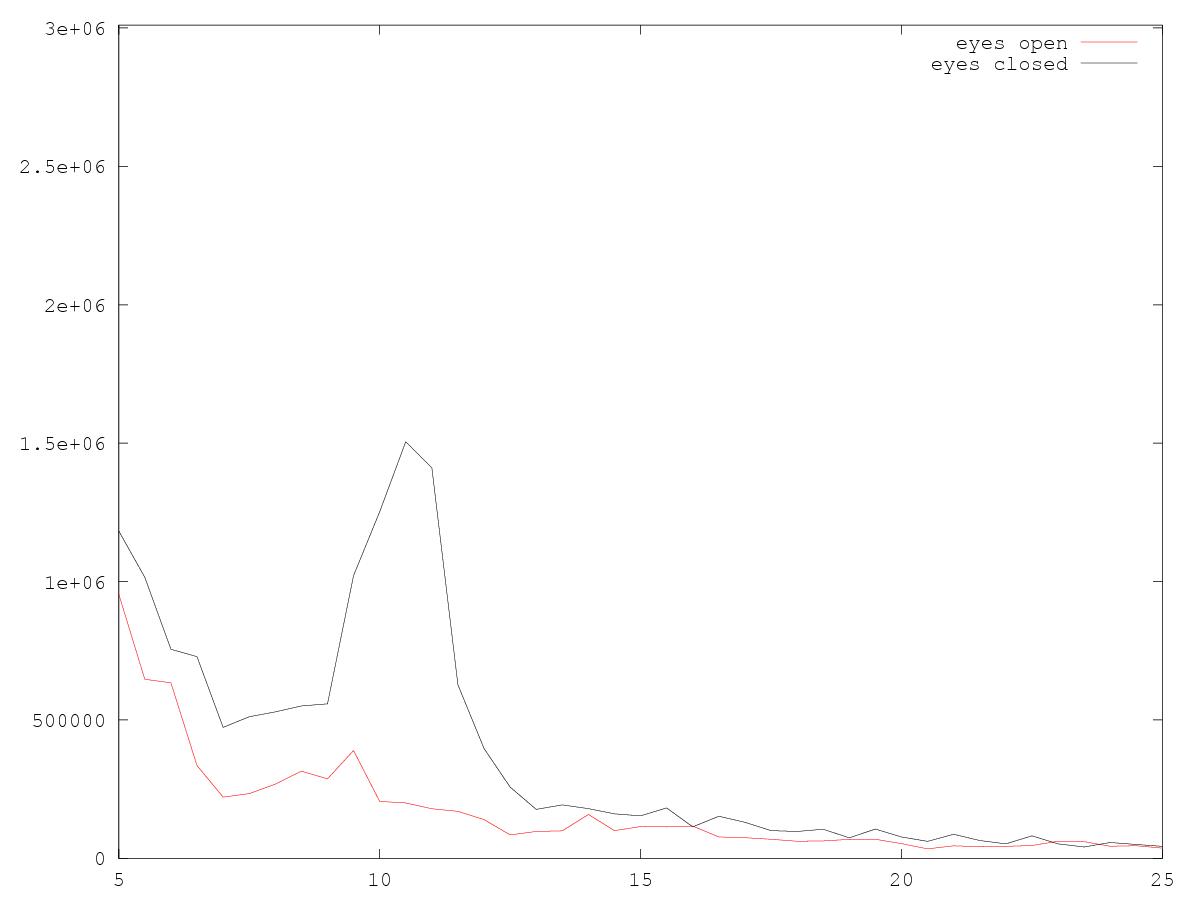
\includegraphics[width=1.000\linewidth]{experiment-final-7-epoc-pwelch-power.png}
\caption[EPOC (pwelch) power.]{EPOC power of each frequency.}\label{ch-experiment/index:fig-experiment-final-7-emotiv-alpha-power}\end{subfigure}
\begin{subfigure}[t]{0.49\linewidth}
\centering
\capstart

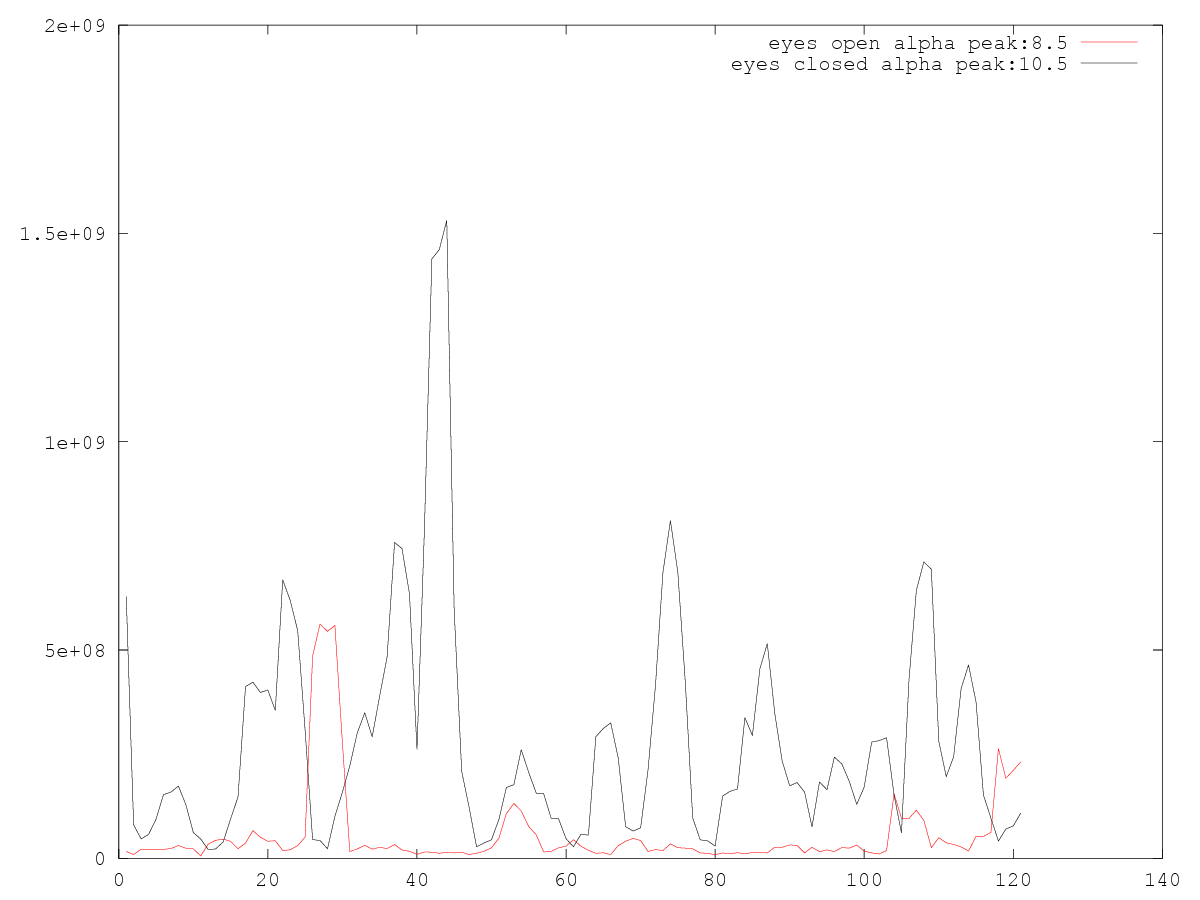
\includegraphics[width=1.000\linewidth]{experiment-final-7-mindwave-alpha-progress.png}
\caption[EPOC alpha progress.]{Mindwave alpha progress. Alpha peaks: 8,5 Hz (open eyes) and 10,5 Hz (closed eyes).}\label{ch-experiment/index:fig-experiment-final-7-mindwave-alpha-progress}\end{subfigure}
\begin{subfigure}[t]{0.49\linewidth}
\centering
\capstart

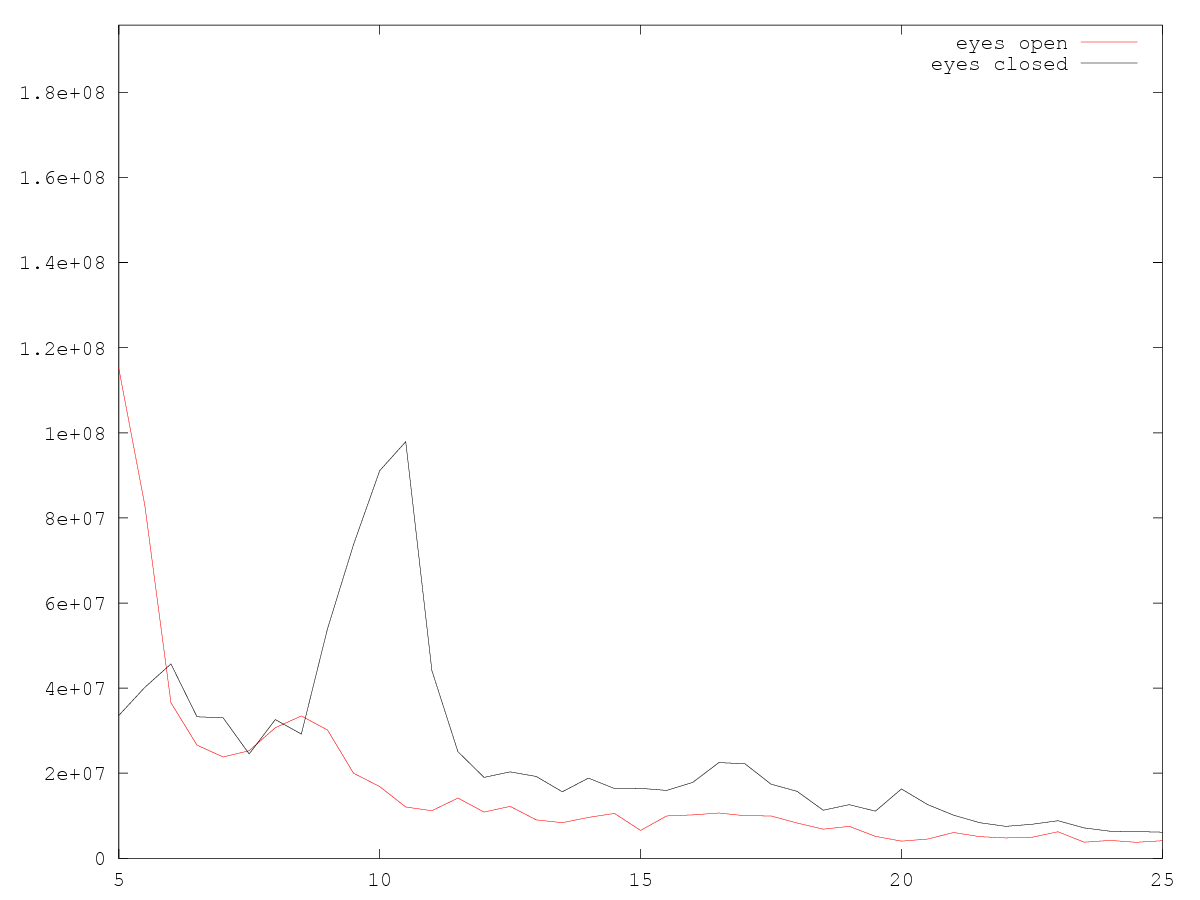
\includegraphics[width=1.000\linewidth]{experiment-final-7-mindwave-pwelch-power.png}
\caption[Mindwave power of each frequency.]{Mindwave power of each frequency.}\label{ch-experiment/index:fig-experiment-final-7-mindwave-alpha-power}\end{subfigure}
\begin{subfigure}[t]{0.49\linewidth}
\centering
\capstart

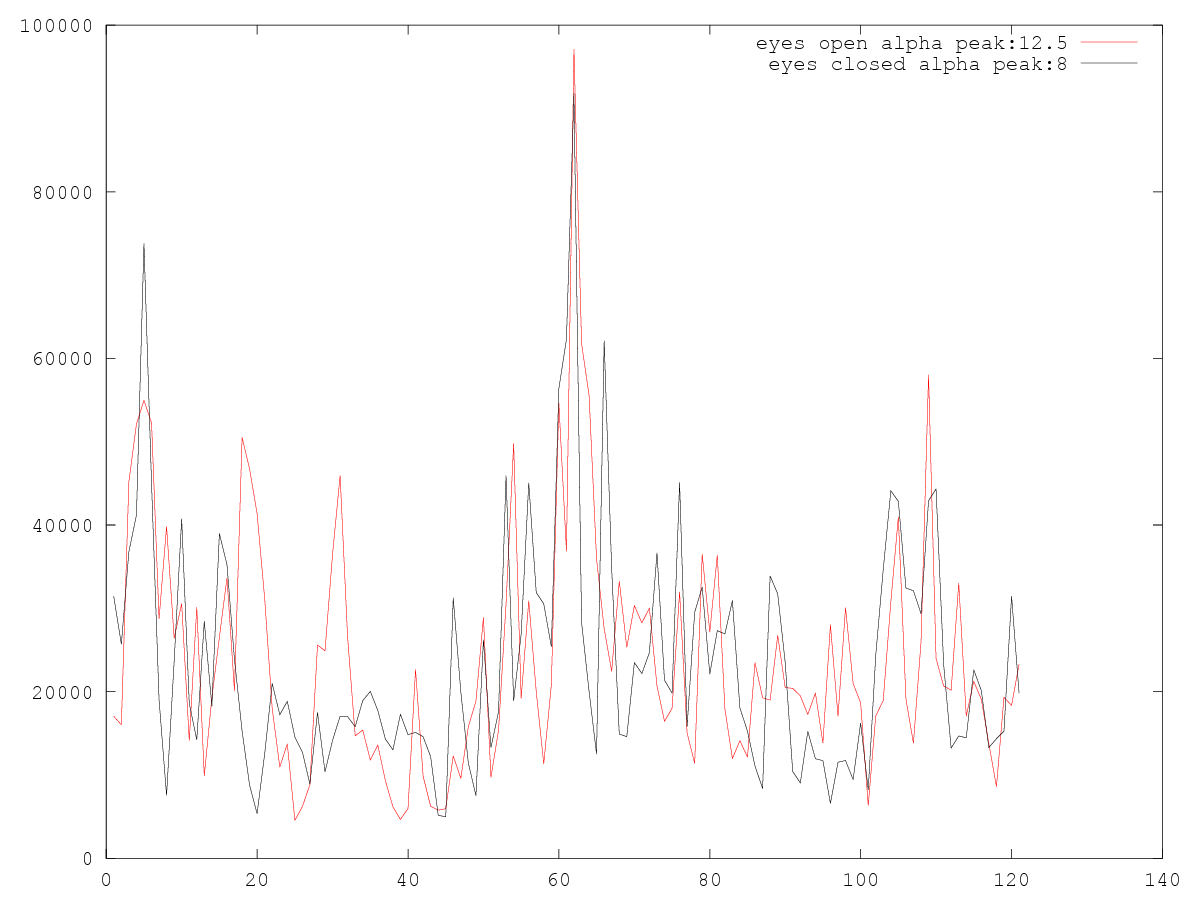
\includegraphics[width=1.000\linewidth]{experiment-final-7-truesense-alpha-progress.png}
\caption[True Sense Kit alpha progress.]{True Sense Kit alpha progress. Alpha peaks: 12,5 Hz (open eyes) and 8 Hz (closed eyes).}\label{ch-experiment/index:fig-experiment-final-7-truesense-alpha-progress}\end{subfigure}
\begin{subfigure}[t]{0.49\linewidth}
\centering
\capstart

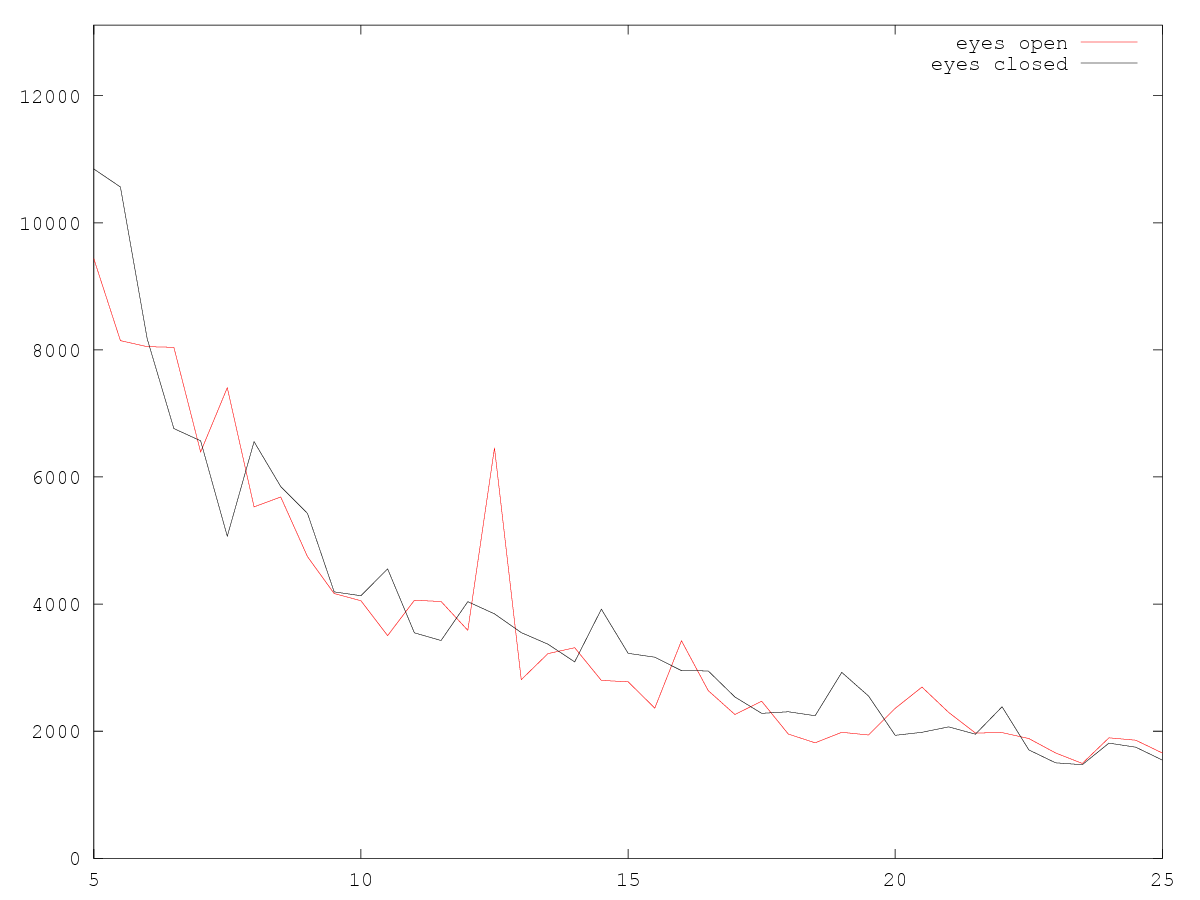
\includegraphics[width=1.000\linewidth]{experiment-final-7-truesense-pwelch-power.png}
\caption[True Sense Kit power of each frequency.]{True Sense Kit power of each frequency. Pay attention to the narrow (noise) peak around 12,5 with open eyes.}\label{ch-experiment/index:fig-experiment-final-7-truesense-alpha-power}\end{subfigure}
\caption[Experiment recording 7]{Plots from recordings of participant 3 from the experiment. On the left, alpha progress
with eyes open (red line) and eyes closed (black line) are plotted. On the right,
the power of each
frequency is plotted - notice the alpha peak around 10 Hz in the EPOC and MindWave
recordings under closed-eyes condition.}\phantomsection\label{ch-experiment/index:fig-final-experiment-recording-7}

\end{figure}


\begin{figure}
\centering
\capstart
\begin{subfigure}[t]{0.49\linewidth}
\centering
\capstart

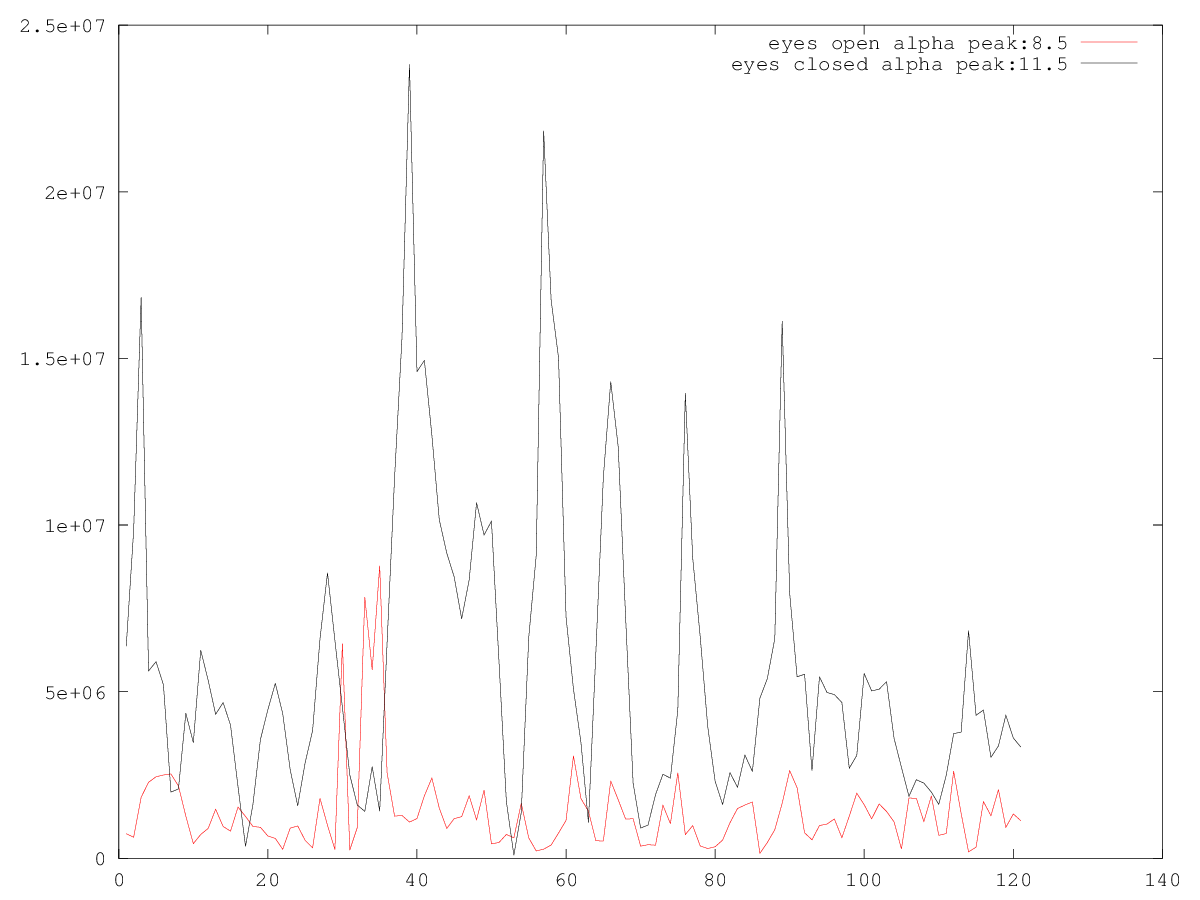
\includegraphics[width=1.000\linewidth]{experiment-final-13-epoc-alpha-progress.png}
\caption[EPOC alpha progress.]{EPOC alpha progress. Alpha peaks: 8,5 Hz (open eyes) and 11,5 Hz (closed eyes).}\label{ch-experiment/index:fig-experiment-final-13-emotiv-alpha-progress}\end{subfigure}
\begin{subfigure}[t]{0.49\linewidth}
\centering
\capstart

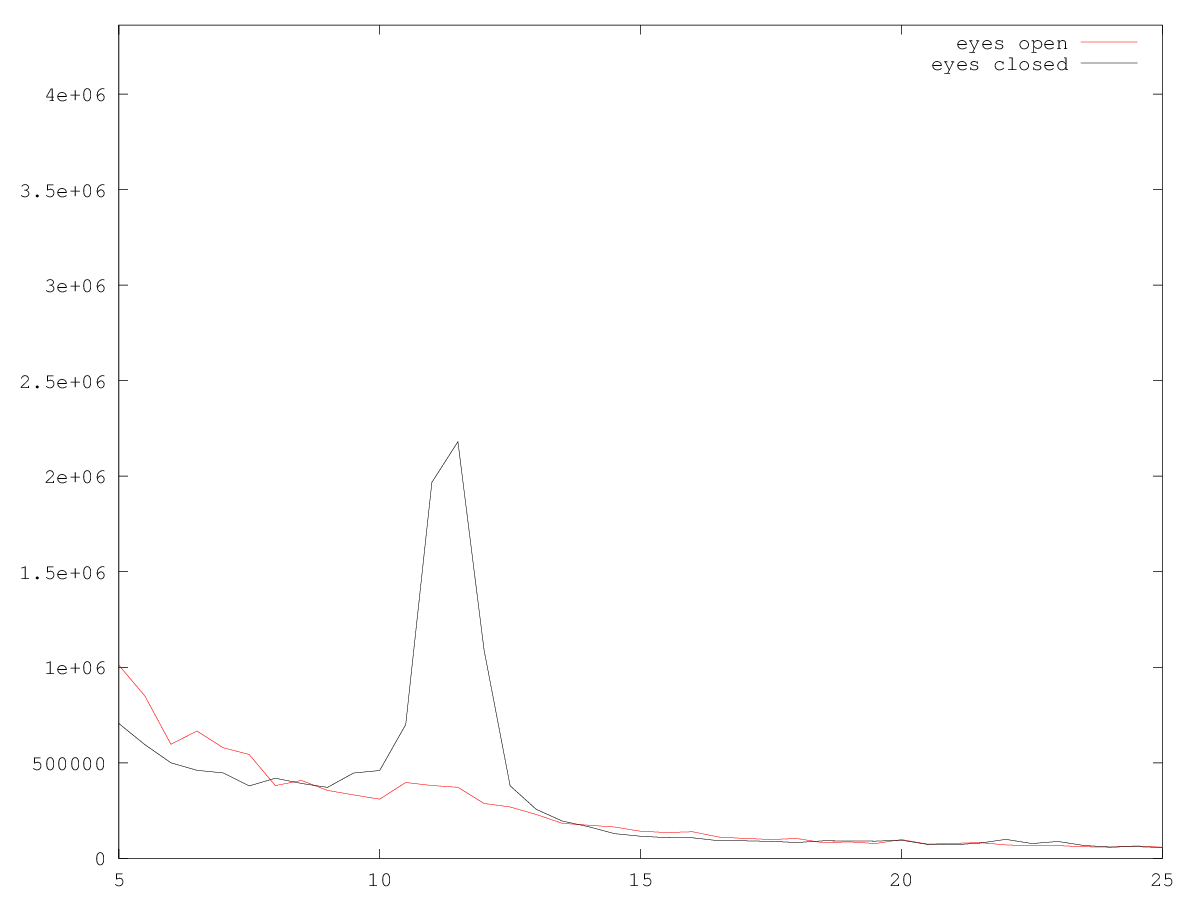
\includegraphics[width=1.000\linewidth]{experiment-final-13-epoc-pwelch-power.png}
\caption[EPOC (pwelch) power.]{EPOC power of each frequency.}\label{ch-experiment/index:fig-experiment-final-13-emotiv-alpha-power}\end{subfigure}
\begin{subfigure}[t]{0.49\linewidth}
\centering
\capstart

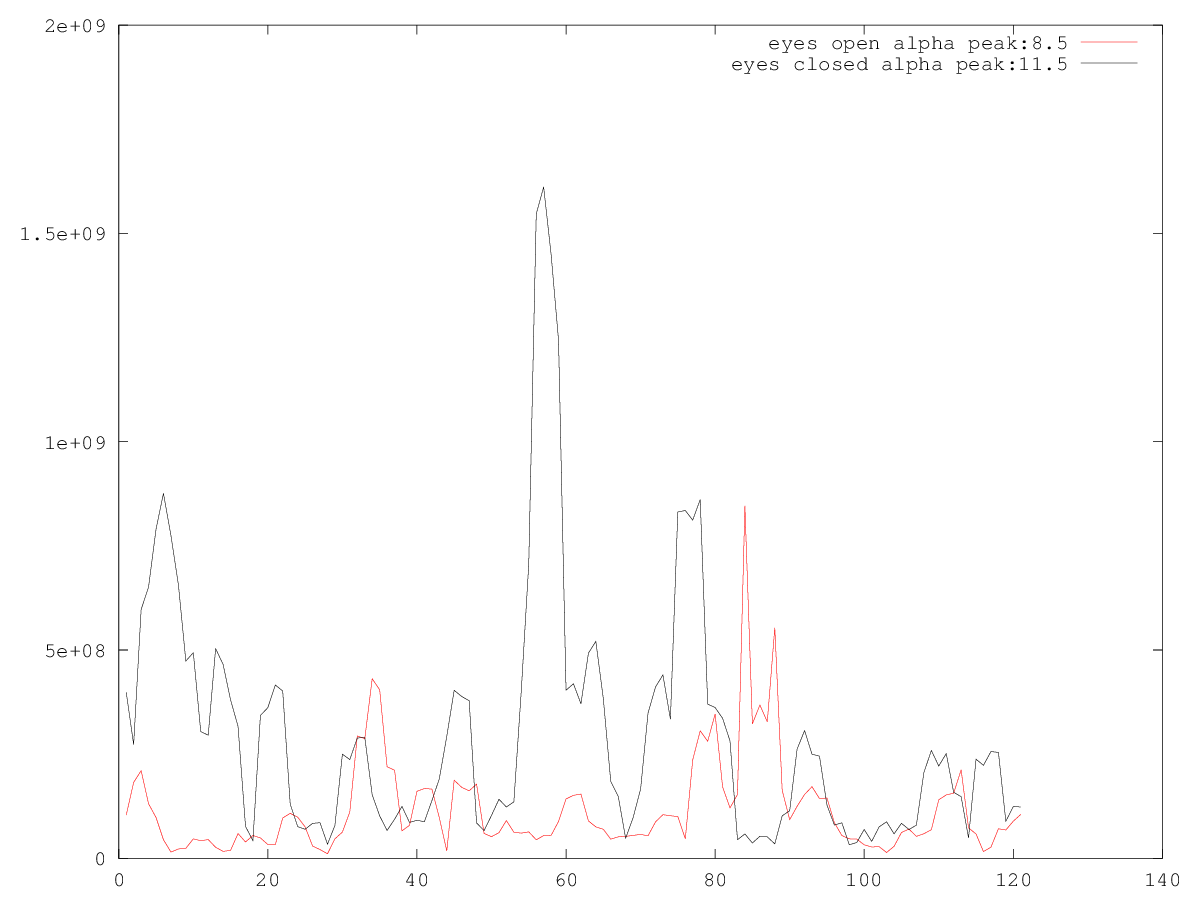
\includegraphics[width=1.000\linewidth]{experiment-final-13-mindwave-alpha-progress.png}
\caption[EPOC alpha progress.]{Mindwave alpha progress. Alpha peaks: 8,5 Hz (open eyes) and 11,5 Hz (closed eyes).}\label{ch-experiment/index:fig-experiment-final-13-mindwave-alpha-progress}\end{subfigure}
\begin{subfigure}[t]{0.49\linewidth}
\centering
\capstart

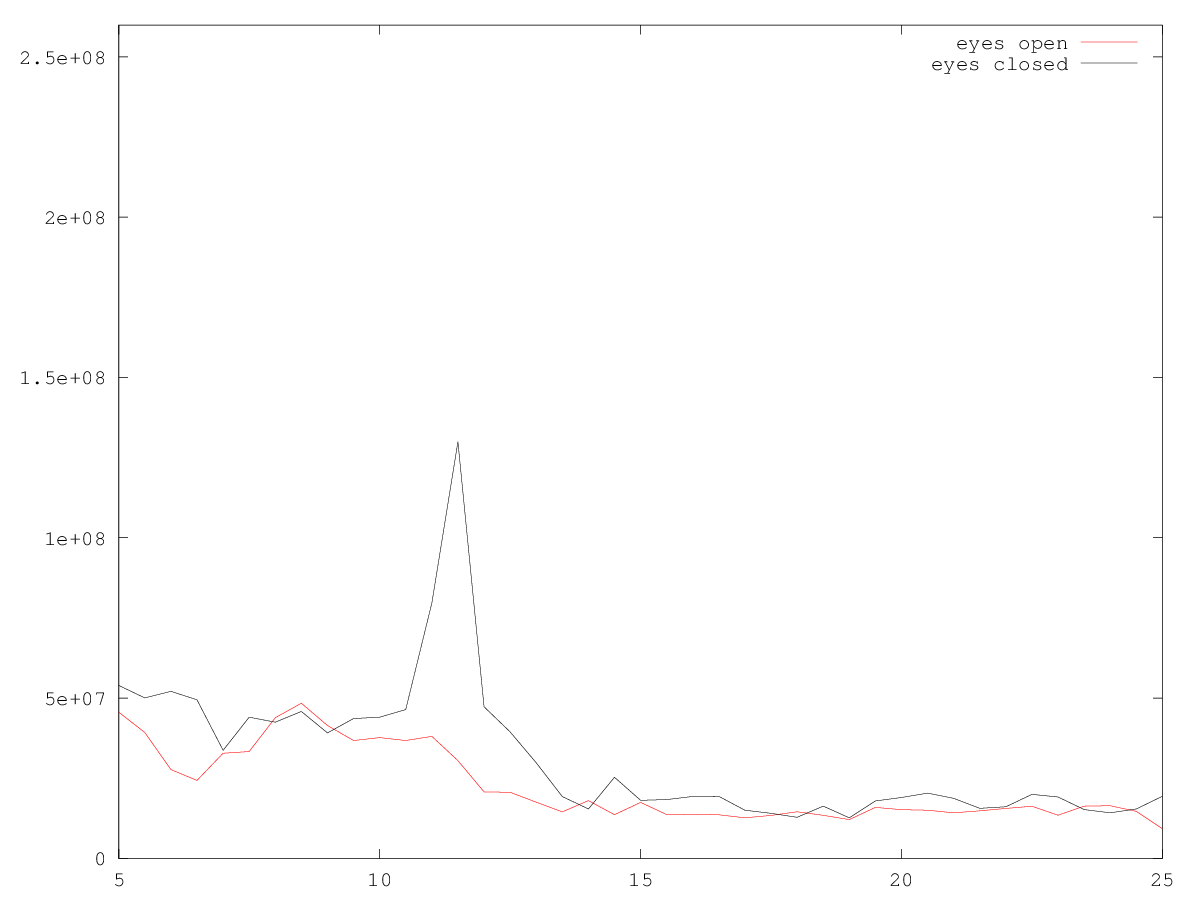
\includegraphics[width=1.000\linewidth]{experiment-final-13-mindwave-pwelch-power.png}
\caption[Mindwave power of each frequency.]{Mindwave power of each frequency.}\label{ch-experiment/index:fig-experiment-final-13-mindwave-alpha-power}\end{subfigure}
\begin{subfigure}[t]{0.49\linewidth}
\centering
\capstart

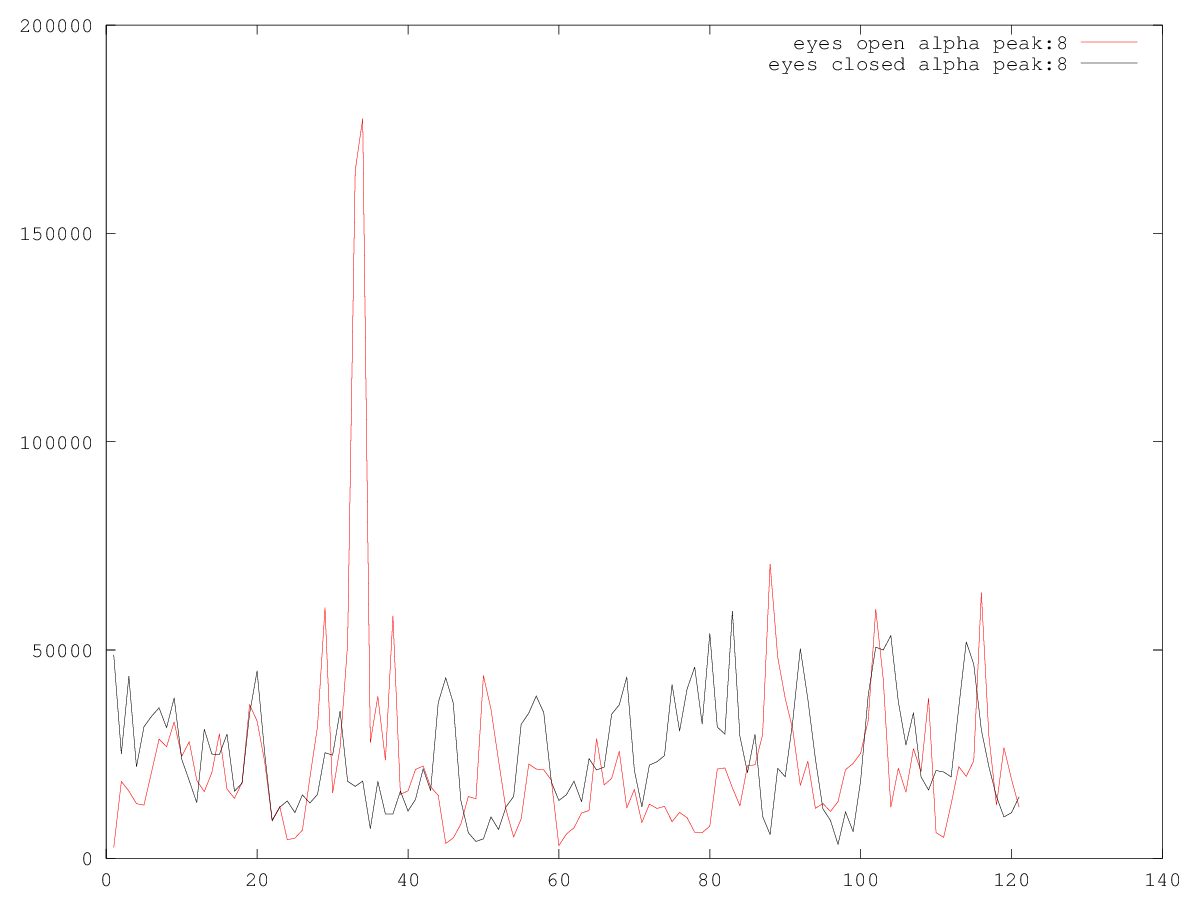
\includegraphics[width=1.000\linewidth]{experiment-final-13-truesense-alpha-progress.png}
\caption[True Sense Kit alpha progress.]{True Sense Kit alpha progress. Alpha peaks: 8 Hz (open eyes) and 8 Hz (closed eyes).}\label{ch-experiment/index:fig-experiment-final-13-truesense-alpha-progress}\end{subfigure}
\begin{subfigure}[t]{0.49\linewidth}
\centering
\capstart

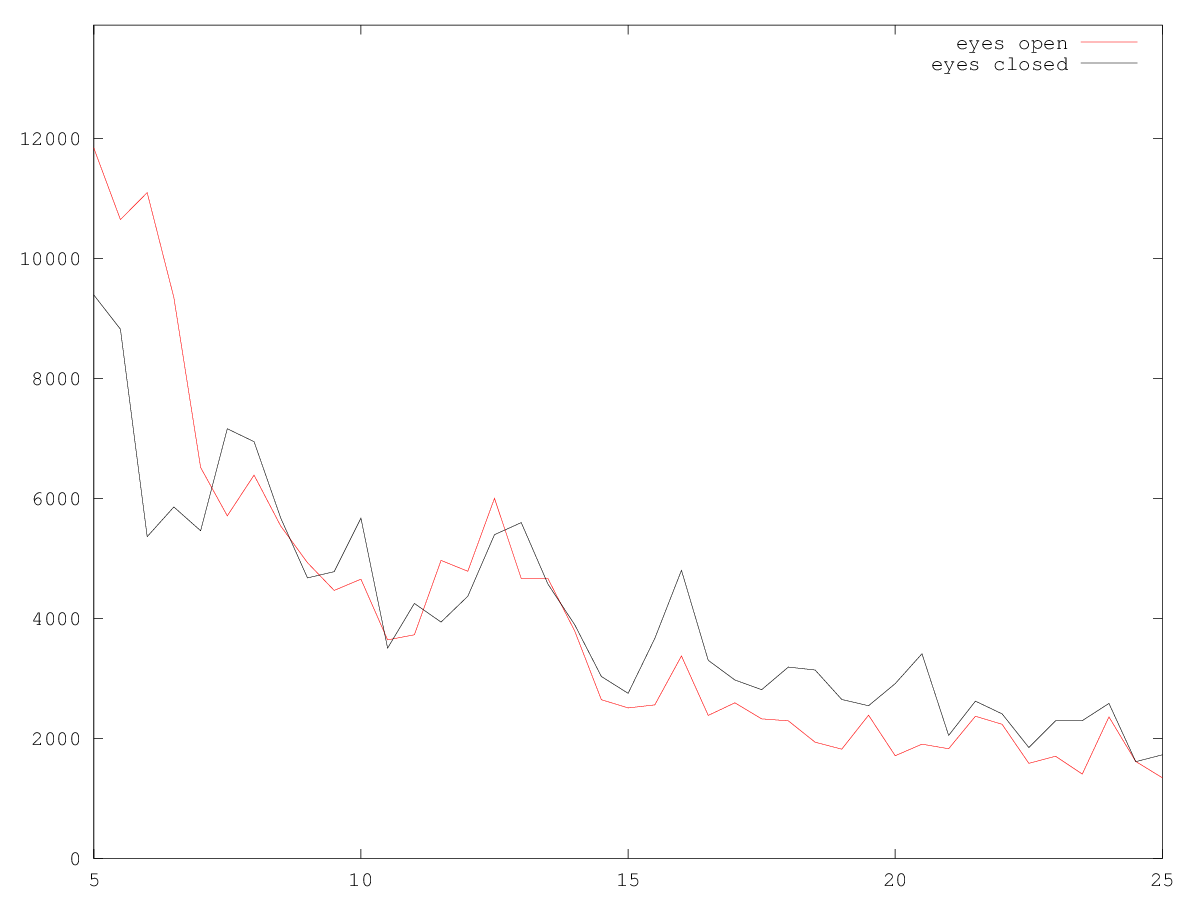
\includegraphics[width=1.000\linewidth]{experiment-final-13-truesense-pwelch-power.png}
\caption[True Sense Kit power of each frequency.]{True Sense Kit power of each frequency.}\label{ch-experiment/index:fig-experiment-final-13-truesense-alpha-power}\end{subfigure}
\caption[Experiment recording 1]{Plots from recordings of participant 5. On the left, alpha progress
with eyes open (red line) and eyes closed (black line) are plotted. On the right,
the power of each
frequency is plotted - notice the alpha peak around 11.5 Hz in the EPOC and MindWave
recordings under closed-eyes condition.}\phantomsection\label{ch-experiment/index:fig-final-experiment-recording-13}

\end{figure}



\section{Choice of BCI}
\label{ch-experiment/index:choice-of-bci}\label{ch-experiment/index:fig-final-experiment-recording-13}
We have lined up the parameters of the evaluation in Table \ref{ch-experiment/index:table-bci-evaluation}. We choose the MindWave BCI in the further
development of AlphaTrainer because: (\emph{i}) it can detect alpha; (\emph{ii}) it does
not require assistance or preparation time to use; (\emph{iii}) it supports Bluetooth
communication; finally (\emph{ii-ii}) it has out of the box SDK support for mobile
devices including access to raw EEG data.

The rationale behind these arguments is based on our overall method which
includes building a system deployable for actual use. In a research context (or
any context requiring spatial resolution), the EPOC is an excellent choice. And
in a quantified-self context in which offline recording and processing is
possible, the TrueSense Kit is the obvious choice due to its size and comfort.

Another advantage of the MindWave is that it seems to best represent the future
of consumer BCIs. As mentioned in Section {\hyperref[ch-background/index:ch-background-future-headsets]{2.2.4}}, the next generation of consumer BCIs
feature Bluetooth connectivity and a dry sensor configuration. By using MindWave
in the further development of AlphaTrainer, we are best prepared for adapting to
future BCIs.


\begin{table}
\capstart
\begin{center}

\bodyspacing

\begin{tabular}{>{\raggedright\arraybackslash}p{0.40\linewidth} p{0.20\linewidth} p{0.20\linewidth} p{0.20\linewidth}}

\toprule
\textsf{\relax } & \textsf{\relax 
EPOC
} & \textsf{\relax 
MindWave
} & \textsf{\relax 
TrueSense Kit
}\\
\hline\midrule

\textbf{Outputs raw EEG}
 & 
(yes)
 & 
yes
 & 
yes
\\

\textbf{Channels}
 & 
14
 & 
1
 & 
1 and up
\\

\textbf{Ability to measure alpha
(1-10)}
 & 
10
 & 
7
 & 
0
\\

\textbf{Preparation time
(minutes)}
 & 
\textgreater{} 10 min
 & 
\textless{} 1 min
 & 
1-5 min
\\

\textbf{Dry sensors}
 & 
No
 & 
Yes
 & 
Yes
\\

\textbf{Comfort to wear (1 - 10)}
 & 
5.67 \(\pm\)2.73
 & 
5.00 \(\pm\)1.67
 & 
8.50 \(\pm\)2.06
\\

\textbf{Bluetooth support}
 & 
no
 & 
yes
 & 
no
\\

\textbf{Mobile SDKs}
 & 
(yes)
 & 
yes
 & 
(yes)
\\
\hline\bottomrule

\end{tabular}
\caption[BCI evaluation]{BCI evaluation}\phantomsection\label{ch-experiment/index:table-bci-evaluation}
\end{center}
\end{table}


\chapter{Design}
\label{ch-design/index:design}\label{ch-design/index::doc}\label{ch-design/index:ch-design}
So far, this thesis has established some important notions that we use as input
to the design of AlphaTrainer: (\emph{i}) from the Background Chapter {\hyperref[ch-background/index:ch-background]{2}} we learned that alpha feedback training can benefit to
reduce stress; (\emph{ii}) from the BCI Evaluation Chapter {\hyperref[ch-experiment/index:ch-experiment]{3}} we learned that the MindWave Mobile BCI is feasible for
building an alpha feedback training system; and (\emph{iii}) in the Introduction
Chapter {\hyperref[ch-intro/index:ch-intro]{1}} we presented our overall method which includes
the need for a robust system deployable for real world use.

These three notions span the design space for building AlphaTrainer. This
chapter first describes the design model and method used and then moves on to
explain some of the important design activities and choices made during the
design process and finally present the design of AlphaTrainer.


\section{Design model and method}
\label{ch-design/index:ch-design-model-and-method}\label{ch-design/index:design-model-and-method}
This section presents the model used throughout the design of AlphaTrainer and
the set of methods used during the design process. We start out by placing the
design problem at hand within a Human-Computer Interaction (HCI) context which
motivates the choice of design model.

The ISO 9241-210:2010 standard for ``Human-centred design for interactive
systems'' states the following about HCI design:

``\emph{The complexity of human-computer interaction means that it is impossible to
specify completely and accurately every detail of every aspect of the
interaction at the beginning of development. Many of the needs and expectations
of users and other stakeholders only emerge {[}...{]} as the designers refine their
understanding of users and their tasks, and as users are better able to express
their needs in response to potential solutions}`` \cite{iso_iso_2010}
Section 4.5 p. 6.

Since we are designing a system which aims to enable a currently non-existing
practice - namely to perform alpha feedback training on a mobile device in an
everyday context - we are certainly struck by the complexity in regard to
specifying user needs up-front.

When designing for ubicomp, additional aspects has to be taken in consideration
which further increase complexity: (\emph{i}) different devices; (\emph{ii}) mobile users;
and (\emph{iii}) changing environment and context \cite{bardram_ubiquitous_2010}. We recognize that we are not only designing
interfaces but also designing interactions between people and the system through
some artifacts embedded in an environment \cite{beaudouin-lafon_designing_2004}. In a neurofeedback training system we
have: (\emph{i}) a user; (\emph{ii}) using artifacts in form of the mobile device and the
headset; and (\emph{iii}) in an environment with a lot of parameters such as noise,
changing lights, other people etc. This requires us to think of the interaction
in context - \emph{in-situ} - at home, at work or somewhere in between (e.g. when
commuting) \cite{benyon_designing_2005} \cite{abowd_human_2002}.

To deal with the complexity and difficulty of specifying user needs and system
requirements up front, we take a user centered approach to our design
process. This approach enables specifications to emerge during the design
process through experiments and prototypes from which we will learn and design
new experiments and prototypes \cite{benyon_designing_2005} \cite{klemmer_how_2006}. We have drawn the model in Figure \ref{ch-design/index:fig-iterative-model}.
\begin{figure}[tbp]
\centering
\capstart

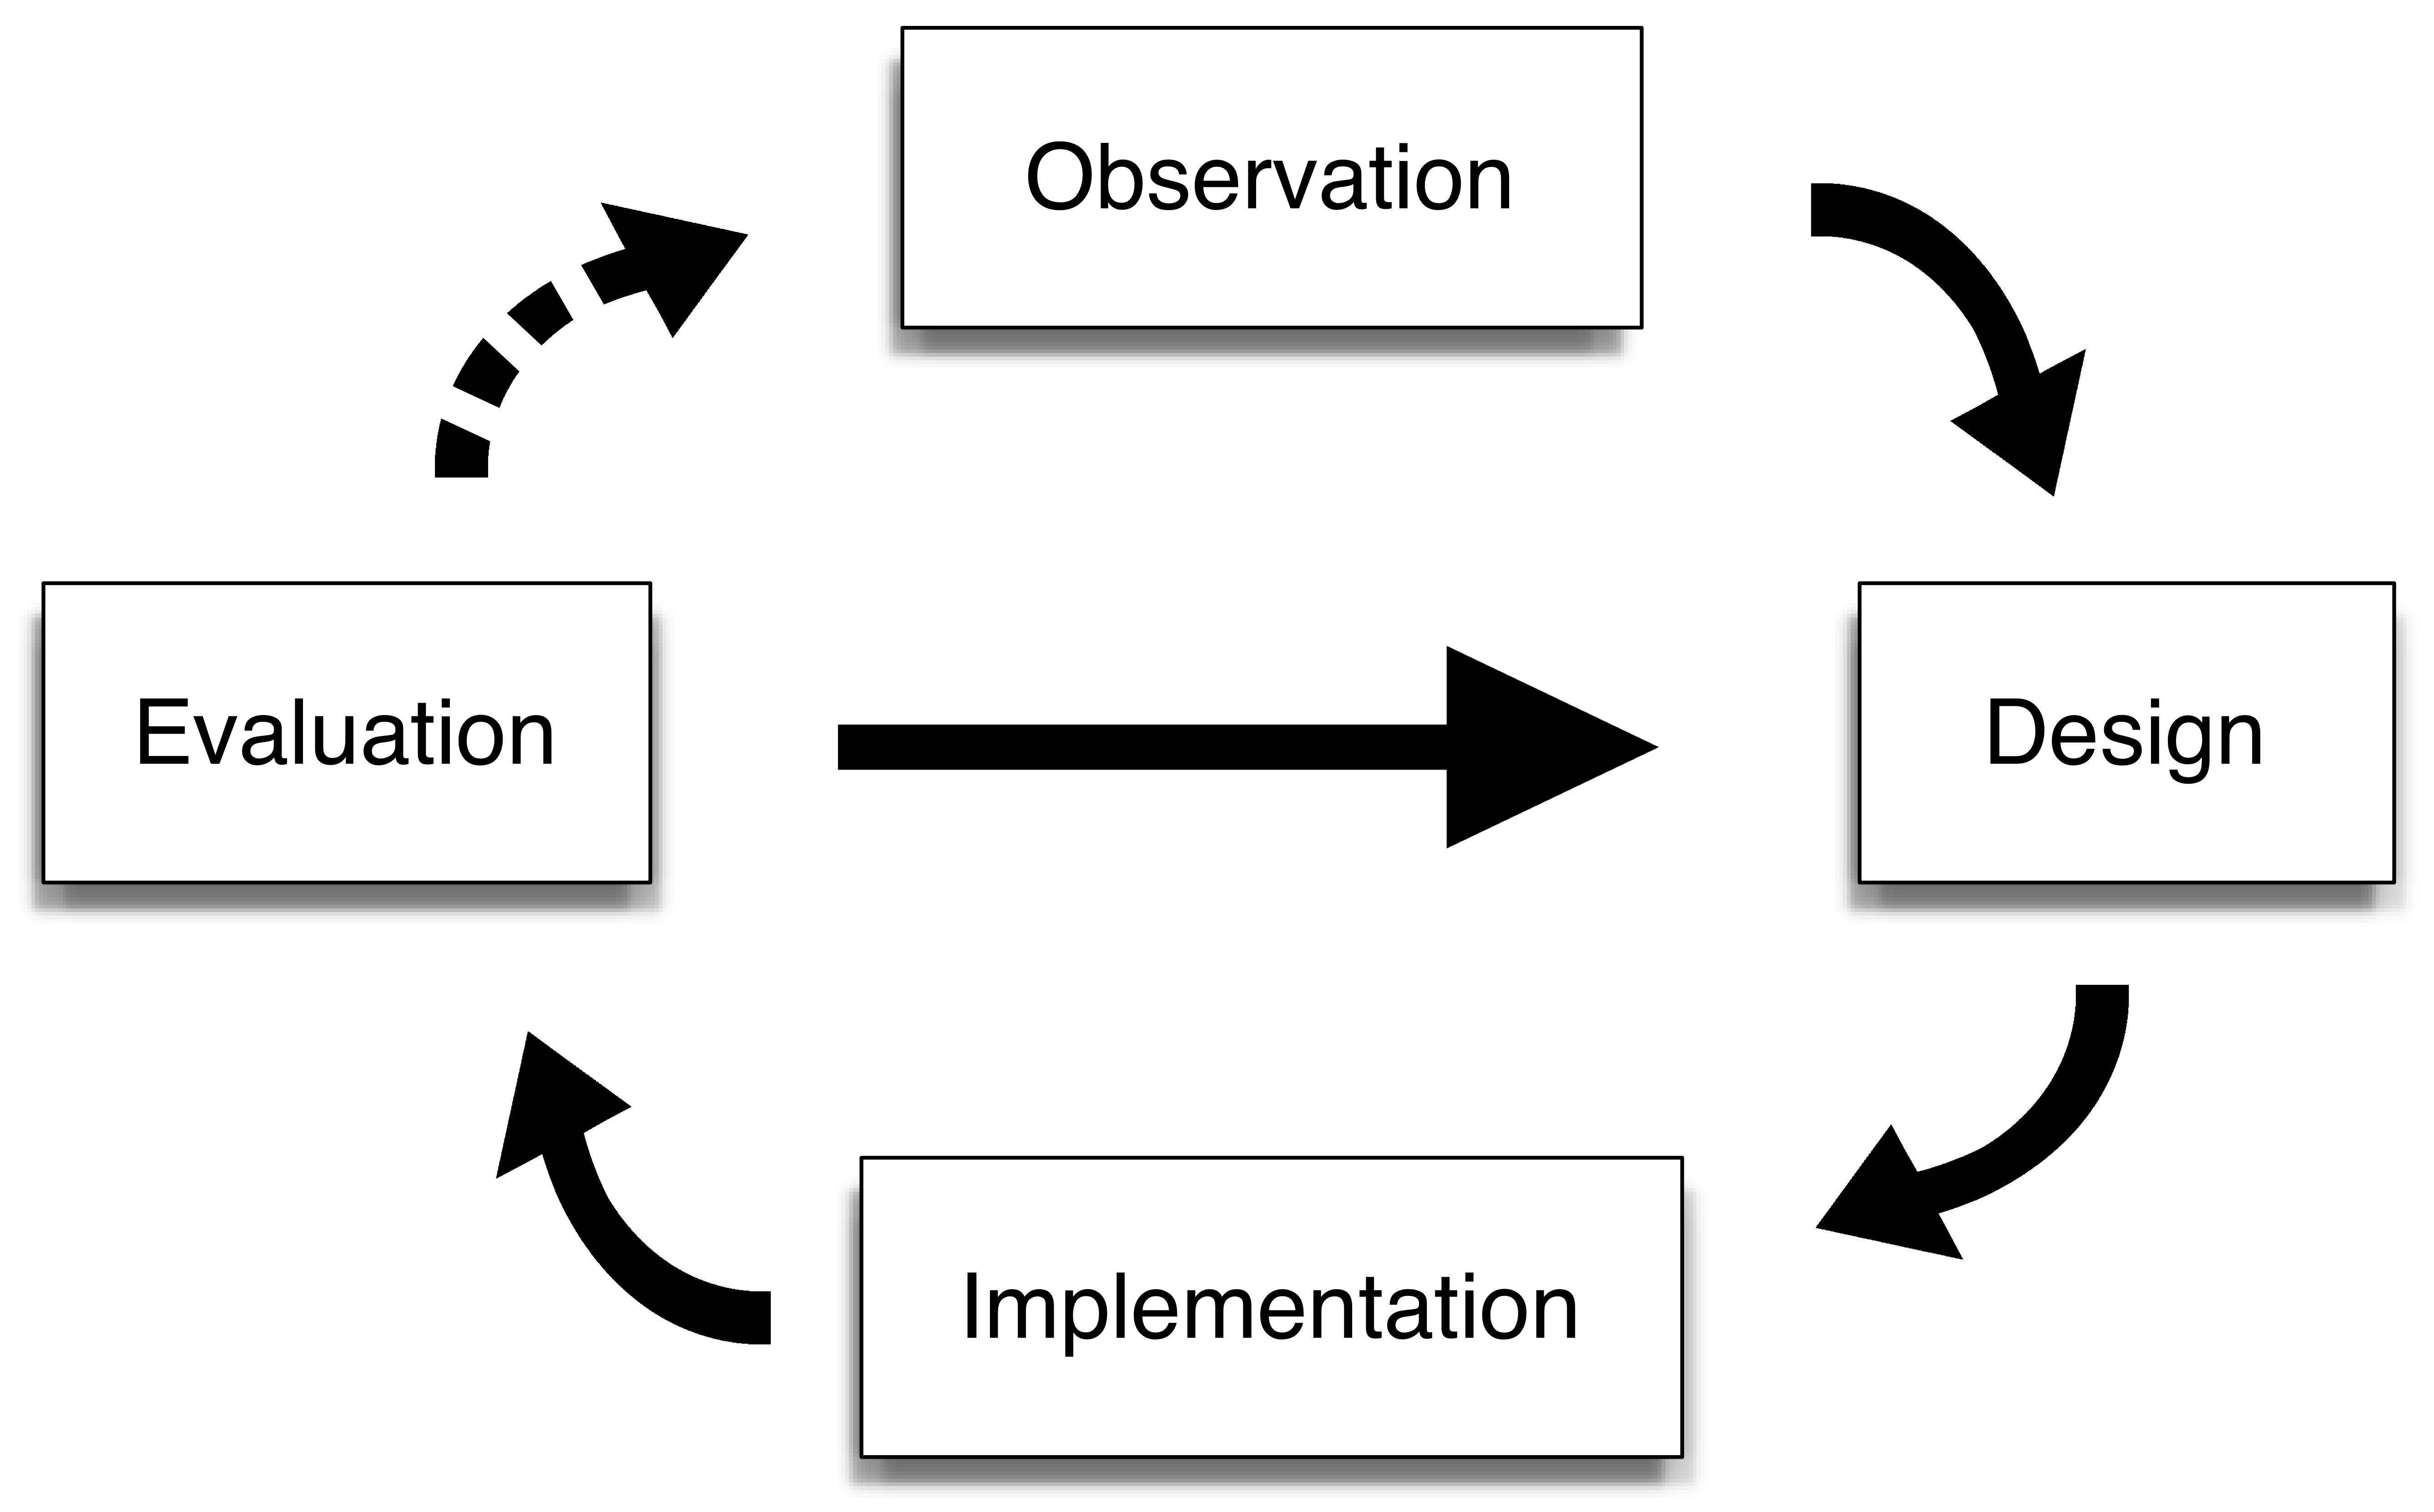
\includegraphics[width=0.600\linewidth]{theiterativemodel.png}
\caption[The iterative model.]{The iterative model.}\label{ch-design/index:fig-iterative-model}\end{figure}

To envision the needs and goals of the users of our system we have been using
personas and scenarios \cite{kollmann_importance_2009}\cite{benyon_designing_2010}. A persona simply model a certain user in order
to delimit the target group for whom we are designing AlphaTrainer. We have
created four personas named Morten, Niels, Olivia and Peter (Appendix {\hyperref[appendix_design_personas:appendix-design-personas]{\emph{Design - personas}}}). We are using scenarios to frame the context
and situation when and where the system is used. As a subset of scenarios we
have worked with some simple storyboards to capture the setting, sequence and
satisfaction of the actual alpha training (Appendix 
{\hyperref[appendix_design_storyboards:appendix-design-storyboards]{\emph{Design - storyboards}}}).

One of the storyboards cover a work scenario and the person could be \emph{Peter}
(Figure \ref{ch-design/index:fig-design-scenario-work}). \emph{Peter} has had a busy day with
a lot of meetings and deadlines waiting around the corner. It is 11.30 and he
realizes that he can squeeze in alpha feedback training just before lunch to get
his mind clear. Peter finds a silent spot in the office space which mostly
consists of big open spaces but luckily there has been arranged some quiet
spots around. He chooses one of the feedbacks with sound because it is
convenient to use when training with earphones in an office environment.
First he does the calibration, then the reference recording as the app
asks for and finally he performs three 5 minutes training sessions in a row. He
improves his alpha during training and finds himself in a relaxed mental state
after the training. Back to work.
\begin{figure}[tbp]
\centering
\capstart

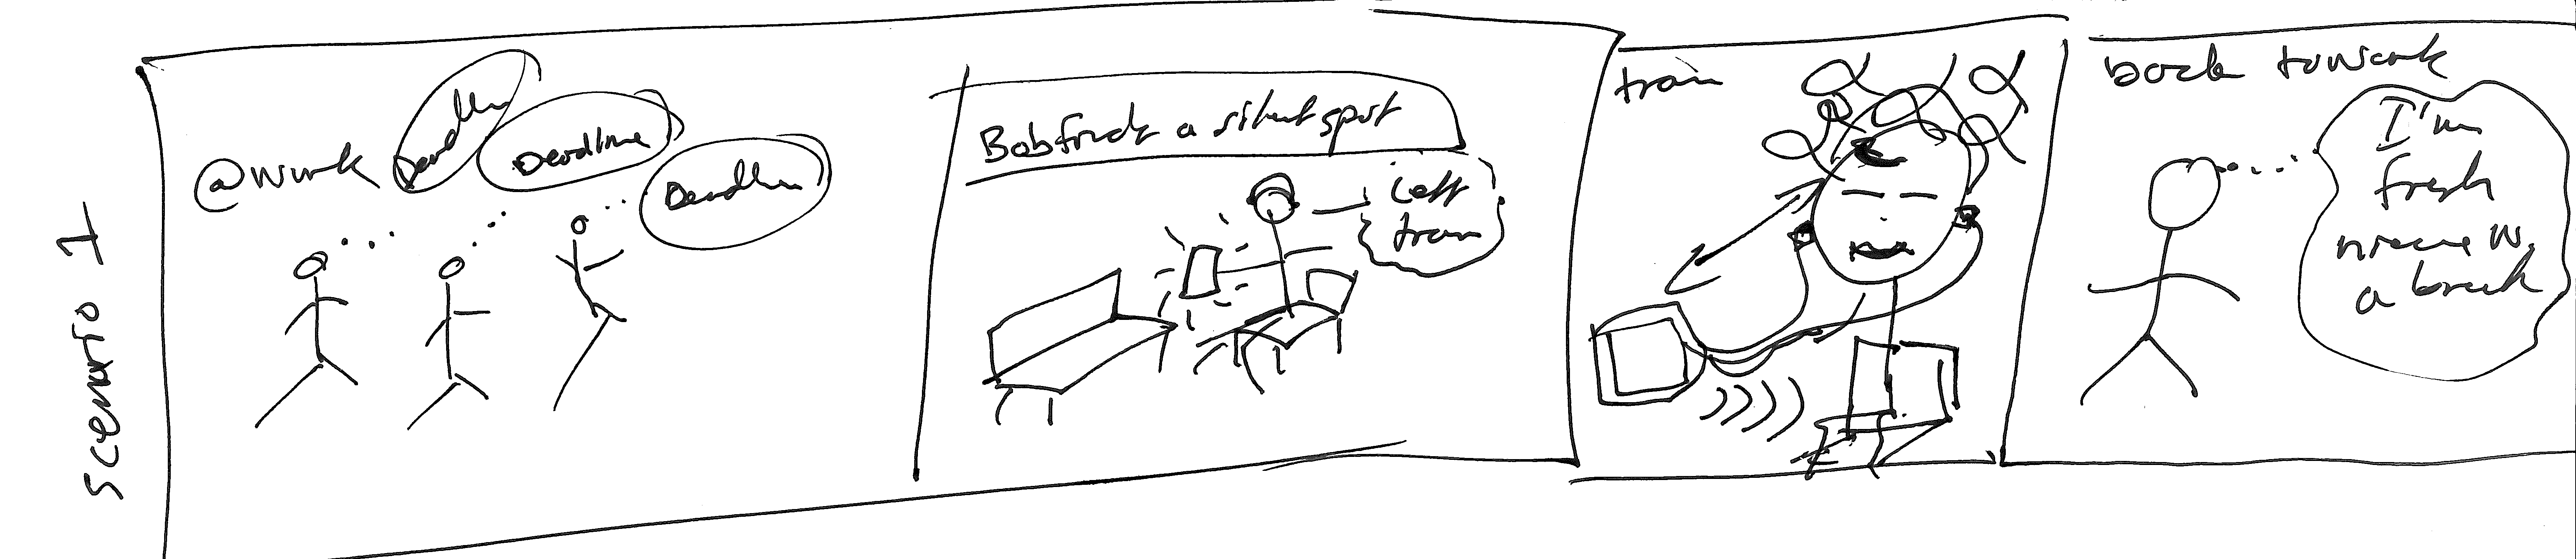
\includegraphics[width=1.000\linewidth]{design-scenario-work1.png}
\caption[Alpha training at work]{Peter performing alpha training at work. Frame 1: Peter has a busy day with a lot of deadlines waiting around the corner. Frame 2: Before lunch, he finds a quiet spot. Frame 3: He performs 15 minutes of alpha training. Frame 4: He finds himself relaxed and gets back to work.}\label{ch-design/index:fig-design-scenario-work}\end{figure}


\section{Design process}
\label{ch-design/index:ch-design-process}\label{ch-design/index:design-process}
Since we have deployed an iterative approach to the design process, we have
decided to present important design activities and decisions
chronologically. This clarifies how we continuously have fed the output of one
design activity as input to another.


\subsection{Initial experimental prototype}
\label{ch-design/index:initial-experimental-prototype}
We started out by making a very simple prototype in the form of an Android app
as proof of concept on getting data from the NeuroSky MindWave Mobile BCI and to
tryout of their SDK signal processing. In a bottom up approach to investigate
what we could control by means of alpha levels, we tried assigning different
audio parameters (volume, pitch, placement in 3D perspective) to the SDK power
band values for low and high alpha. The power band values are listed in Section {\hyperref[ch-background/index:ch-background-mindwave]{2.2.2}}.

We tried out the prototype informally on our selves and on fellow students and
learned that the SDK alpha values contained giant outliers as already mentioned
in the BCI Evaluation Chapter {\hyperref[ch-experiment/index:ch-experiment]{3}}. Besides, we were
unsure whether to use the low alpha or high alpha frequency band from the SDK
since the literature states - as explained in Section {\hyperref[ch-background/index:sec-background-stress-alpha-feedback-training]{2.3.2}} - that the alpha band
varies between individuals and that neurofeedback is significantly more
effective when the feedback is given on individually adapted frequency bands.

In researching how neurofeedback is practiced, we contacted Ann-Helen
Pettersen - one of the few Danish psychiatrists specializing in neurofeedback
therapy \footnote{
\href{http://www.hjernetraening.dk}{http://www.hjernetraening.dk}
}.  She also stressed the
importance of accounting for individually determined frequency bands.  When
practicing neurofeedback therapy, she starts out by recording a map of EEG
frequency intensities. This ``brain map'', as she calls it, serves as input to the
choice of an appropriate feedback frequency band.

Based on the notions from the literature on alpha feedback training backed up by a
clinician's neurofeedback practice, we decided that our alpha training system
would need the ability to give feedback on an alpha band adapted to the
individual alpha peak frequency. This led us to experiment with doing the
frequency analysis our selves. This
also enabled us to test whether we could reproduce the outliers experienced from
the SDK alpha values which would inform about whether they originated from the
raw data or from the SDK processing.

We did the signal processing offline (see Section {\hyperref[ch-experiment/index:ch-experiment-pre-study]{3.1}}) and interestingly we were not able to reproduce
the outliers we got from the SDK. Another interesting find during the data
analysis was that the alpha wave intensity comes in chunks of a few seconds
length as can be seen, for example, in Figure \ref{ch-experiment/index:fig-experiment-final-7-mindwave-alpha-progress}.  The chunks of high alpha
activity can even be observed directly from a raw EEG signal such as the one
shown in Figure \ref{ch-background/index:fig-eeg-with-alpha-waves}.


\subsection{Early functioning Android prototype}
\label{ch-design/index:early-functioning-android-prototype}
As the next step we implemented a working Android alpha feedback training
prototype. We focused on the needs for custom signal processing revealed in our
previous prototype experiments and from the literature. Our approach to signal
processing is covered in the Implementation Chapter {\hyperref[ch-implementation/index:ch-implementation]{5}}. We also created a set of 5 different feedback views
inspired by other neurofeedback systems.

The views were variations over a bar changing height and a box changing
color. We read about the bar feedback in \cite{larsen_classification_2011} describing its clinical usage in ADHD
treatment. The goal for the trainee is to raise the bar which in our case
represents the magnitude of alpha waves. The basic bar feedback is shown in
Figure \ref{ch-design/index:fig-early-prototype-feedback-bar}. The feedback consisting
of a box changing colors was used in the Smartphone Brain Scanner alpha feedback
training application as mentioned in the Background Chapter {\hyperref[ch-background/index:ch-background]{2}}. In our case, the
box gradually change from red over yellow to green. The trainees goal is to make
and keep the box green which represents high alpha magnitude. The basic bar
feedback is shown in Figure \ref{ch-design/index:fig-early-prototype-feedback-box}. Inspired by the Smartphone Brain
Scanner alpha feedback training app (Section {\hyperref[ch-background/index:ch-background-smartphone-brain-scanner-2]{2.4.3}}) - which included another
feedback in which performance history was visible - we implemented a version of
each interface showing recent performance history of a sliding time frame of 30
seconds.

In the case of the box feedback, history was visible in the frame color - see
Figure \ref{ch-design/index:fig-early-prototype-feedback-box-w-history}. In the case of
the bar, we implemented performance history in the form of a horizontal line
showing performance history of a 30 seconds sliding time frame. Additionally, we
visualized performance history of the entire training session in the form of
background color changes - see Figure \ref{ch-design/index:fig-early-prototype-feedback-bar-w-history}. From our initial experience
with the feedback bar, we thought the rather violent movements from low to high
due to the intrinsic variance in alpha magnitude might introduce EOG
noise. Therefor we made another variation of the bar interface in which the bar
only grows. High alpha magnitudes makes it grow fast while low alpha magnitudes
slows the growing down or stops it completely (Figure \ref{ch-design/index:fig-early-prototype-feedback-bar-growing}).

In sum, the prototype featured: (\emph{i}) alpha feedback training through 5
different feedback views; (\emph{ii}) individual alpha peak detection; (\emph{iii}) alpha
feedback training based on flexible alpha band definition; and (\emph{ii-ii}) a view
showing performance history in a plot (Figure \ref{ch-design/index:fig-early-prototype-screen-history}).

Using the app relied on the following sequence of actions:
\begin{enumerate}
\item {} 
The user should turn on and mount the MindWave BCI and launch the Android
application prototype.

\item {} 
The user should calibrate according to the individual alpha peak which is
done by pushing the ``Calibrate'' button. The alpha peak frequency is used to
delimit the alpha band for which to give feedback on.

\item {} 
The user should record a baseline while under influence of random feedback
which is done by pushing the ``Baseline'' button. The baseline is used in
mapping the current alpha level to a feedback state. Furthermore, the
baseline recordings are used to track alpha activity gains over time, the
\emph{training effect} of using AlphaTrainer.

\item {} 
The app is now ready for training which is started by pushing the ``Feedback''
button.

\end{enumerate}

The prototype app uses standard Android UI components (see Figure \ref{ch-design/index:fig-early-prototype-app-screen-start}) and the interaction form is manual
as it is clear from the training procedure listed above. In designing and
building the prototype we thought in terms of \emph{availability} regarding app
functionality and the information dimensions present in the feedbacks (for
example feedbacks showing current alpha state + performance history).

\begin{figure}
\centering
\capstart
\begin{subfigure}[t]{0.30\linewidth}
\centering
\capstart

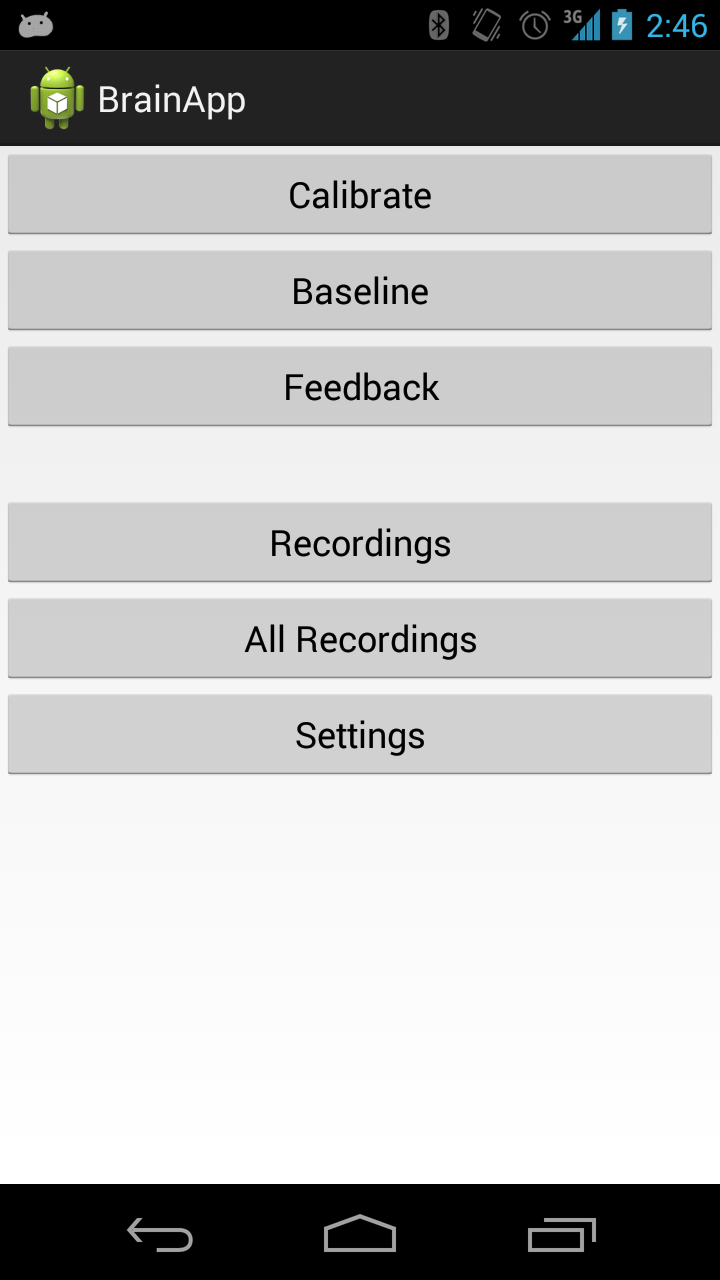
\includegraphics[width=0.800\linewidth]{early-prototype-app-screen-start.png}
\caption[Start screen]{Early prototype app screen start.}\label{ch-design/index:fig-early-prototype-app-screen-start}\end{subfigure}
\begin{subfigure}[t]{0.30\linewidth}
\centering
\capstart

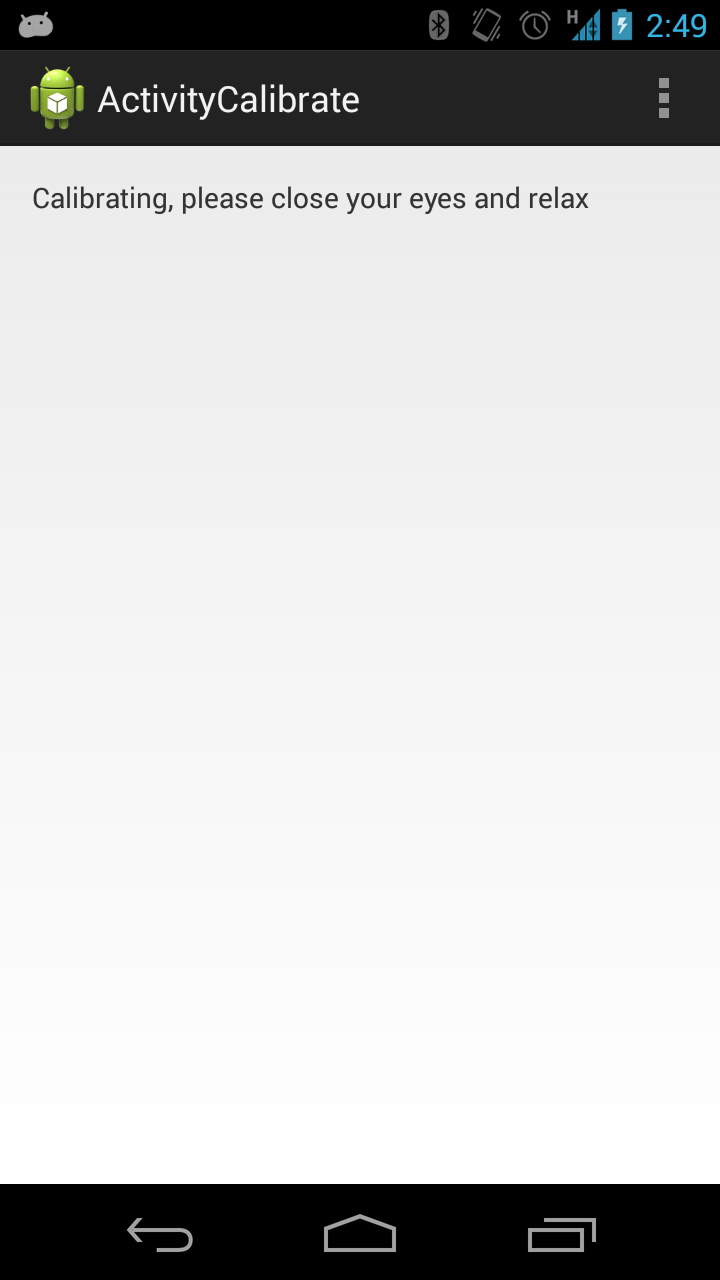
\includegraphics[width=0.800\linewidth]{early-prototype-screen-calibrate.png}
\caption[Calibration screen]{Calibration screen.}\label{ch-design/index:fig-early-prototype-screen-calibrate}\end{subfigure}
\begin{subfigure}[t]{0.30\linewidth}
\centering
\capstart

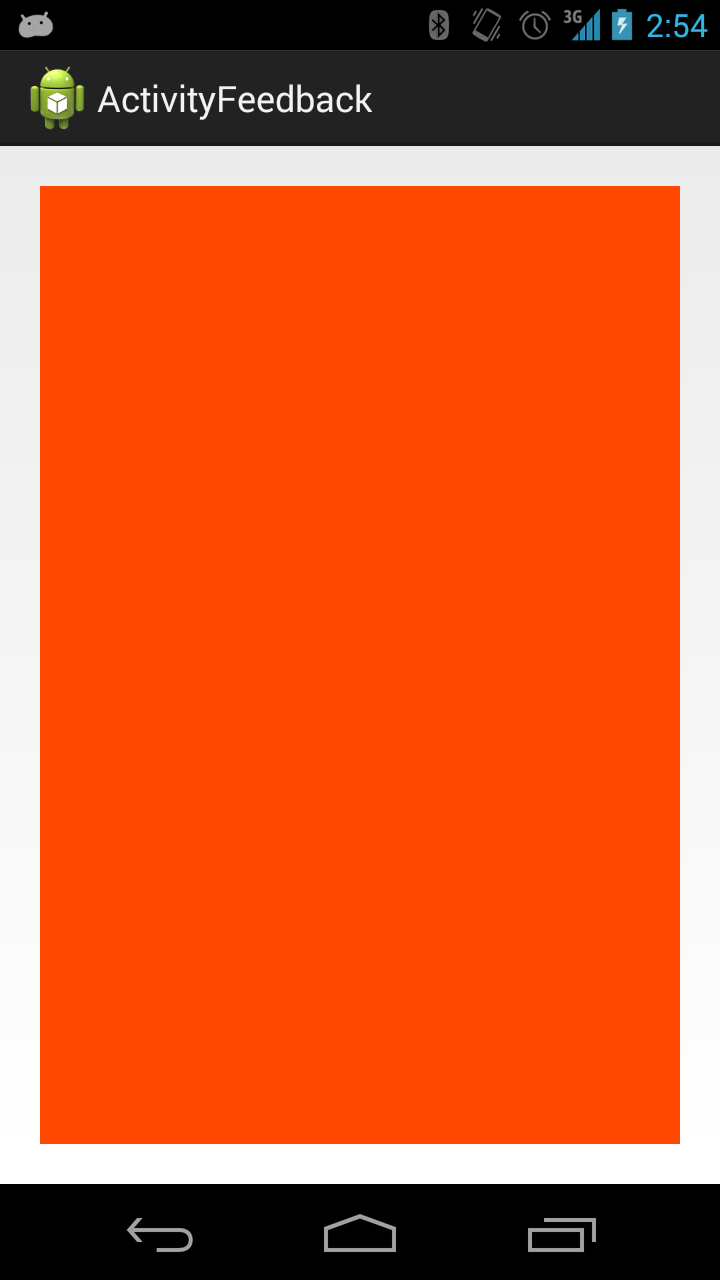
\includegraphics[width=0.800\linewidth]{early-prototype-feedback-box.png}
\caption[Feedback box]{Feedback box.}\label{ch-design/index:fig-early-prototype-feedback-box}\end{subfigure}
\begin{subfigure}[t]{0.30\linewidth}
\centering
\capstart

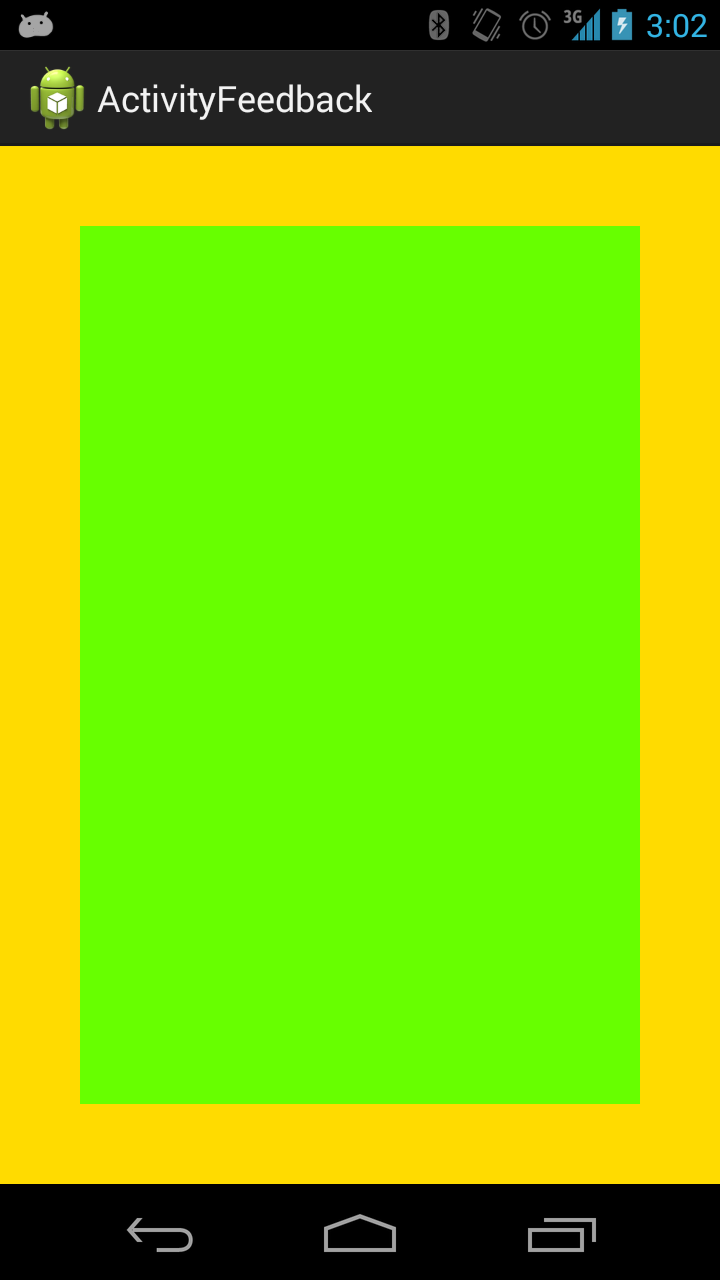
\includegraphics[width=0.800\linewidth]{early-prototype-feedback-box-w-history.png}
\caption[Feedback box with history]{Feedback box with history. Green is current feedback and border is history.}\label{ch-design/index:fig-early-prototype-feedback-box-w-history}\end{subfigure}
\begin{subfigure}[t]{0.30\linewidth}
\centering
\capstart

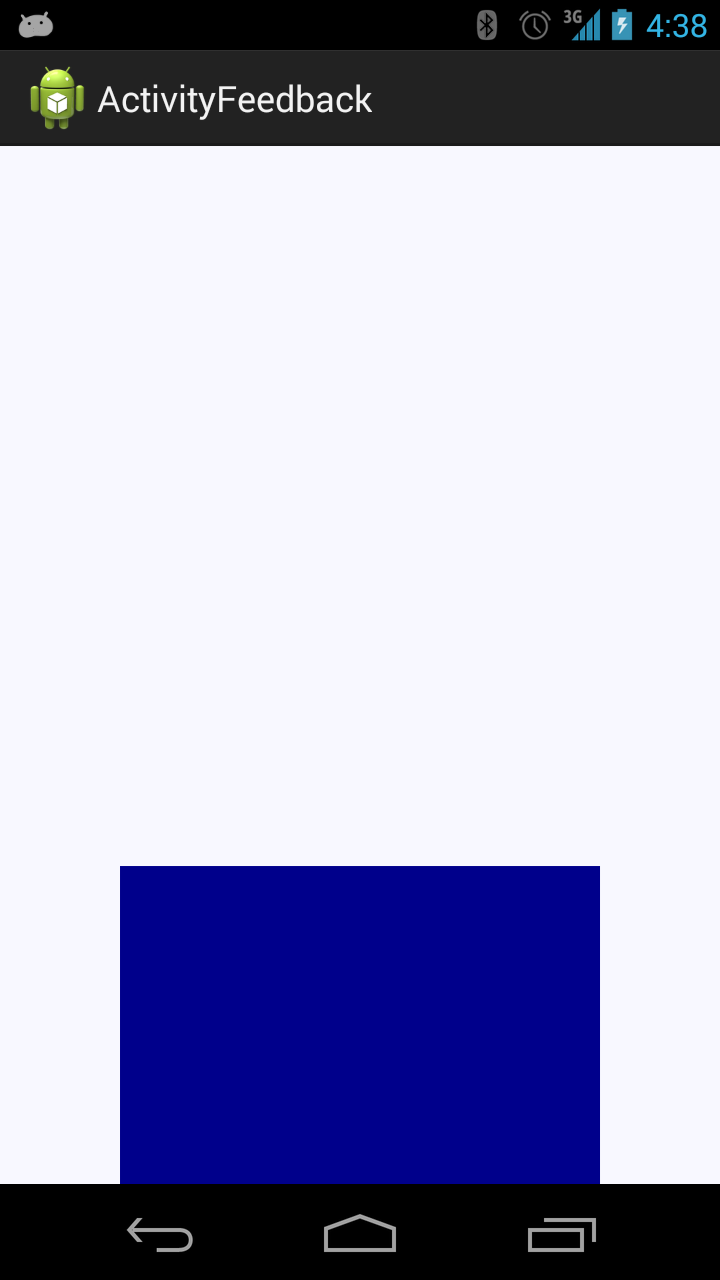
\includegraphics[width=0.800\linewidth]{early-prototype-feedback-bar.png}
\caption[Feedback bar]{Feedback bar goes up and down based on alpha level.}\label{ch-design/index:fig-early-prototype-feedback-bar}\end{subfigure}
\begin{subfigure}[t]{0.30\linewidth}
\centering
\capstart

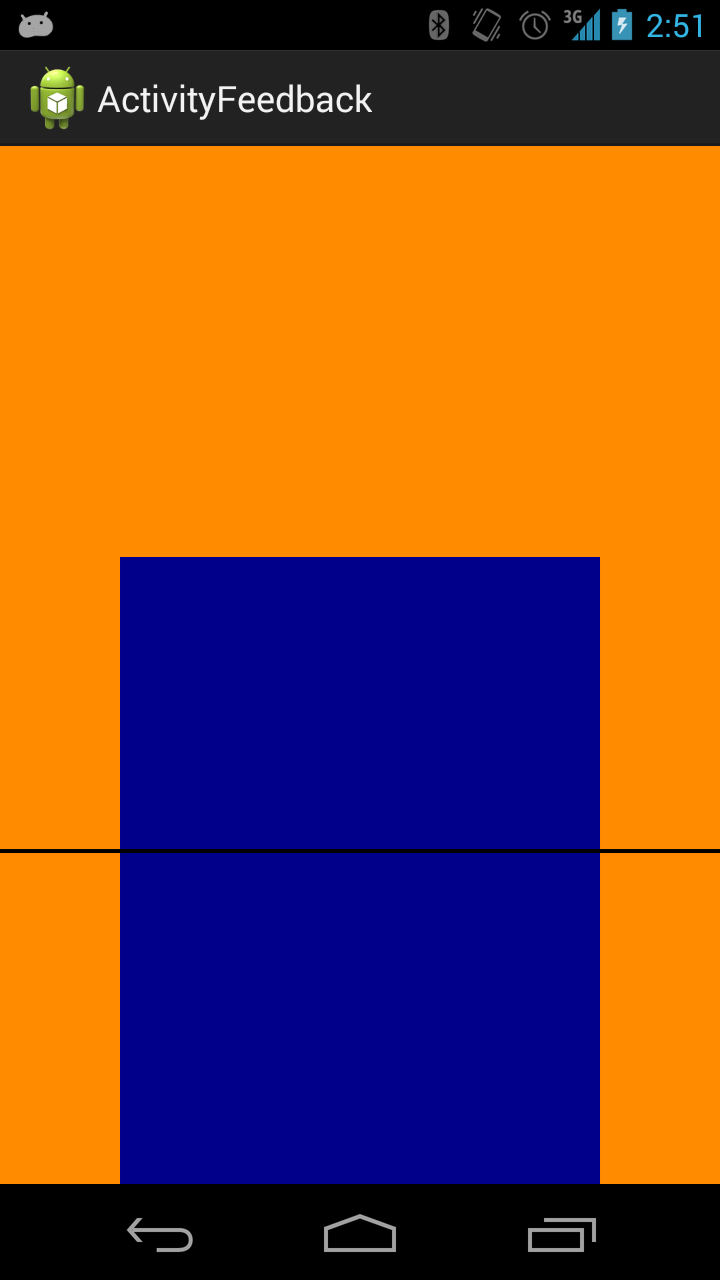
\includegraphics[width=0.800\linewidth]{early-prototype-feedback-bar-w-history.png}
\caption[Feedback bar with history]{Feedback bar with history.}\label{ch-design/index:fig-early-prototype-feedback-bar-w-history}\end{subfigure}
\begin{subfigure}[t]{0.30\linewidth}
\centering
\capstart

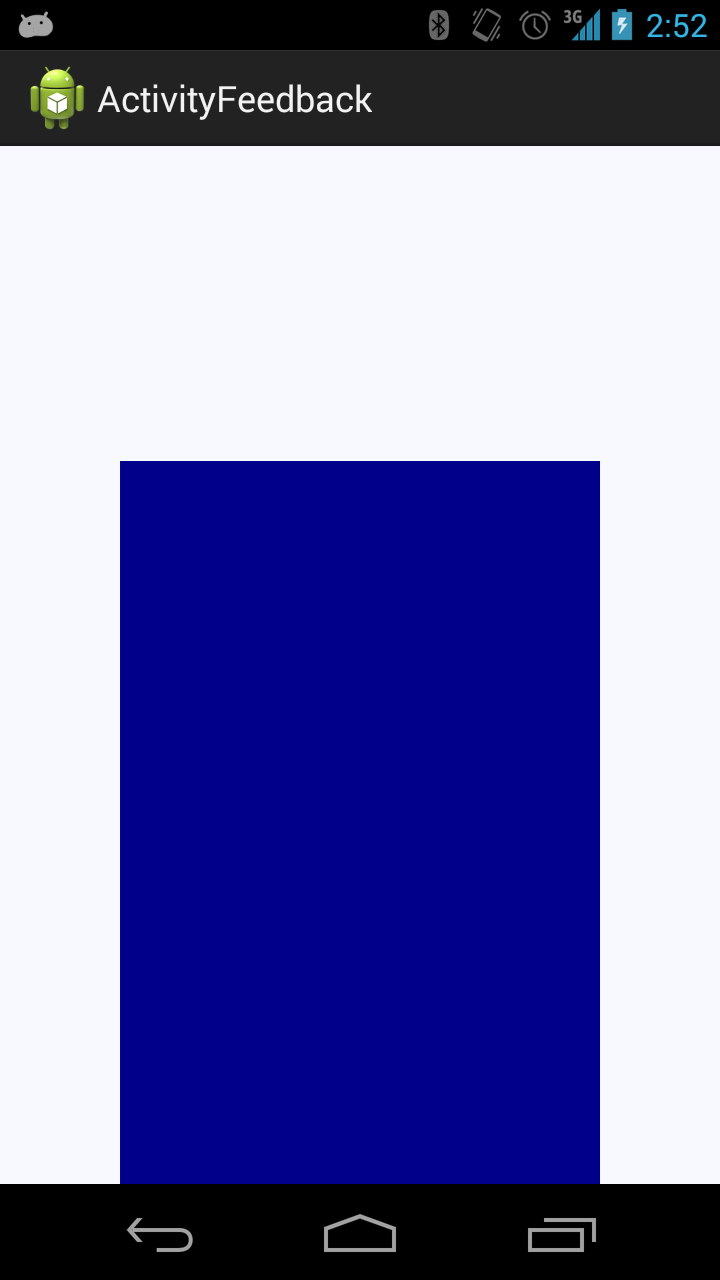
\includegraphics[width=0.800\linewidth]{early-prototype-feedback-bar-growing.png}
\caption[Feedback bar growing]{Feedback bar growing gradually based on the summed alpha.}\label{ch-design/index:fig-early-prototype-feedback-bar-growing}\end{subfigure}
\begin{subfigure}[t]{0.30\linewidth}
\centering
\capstart

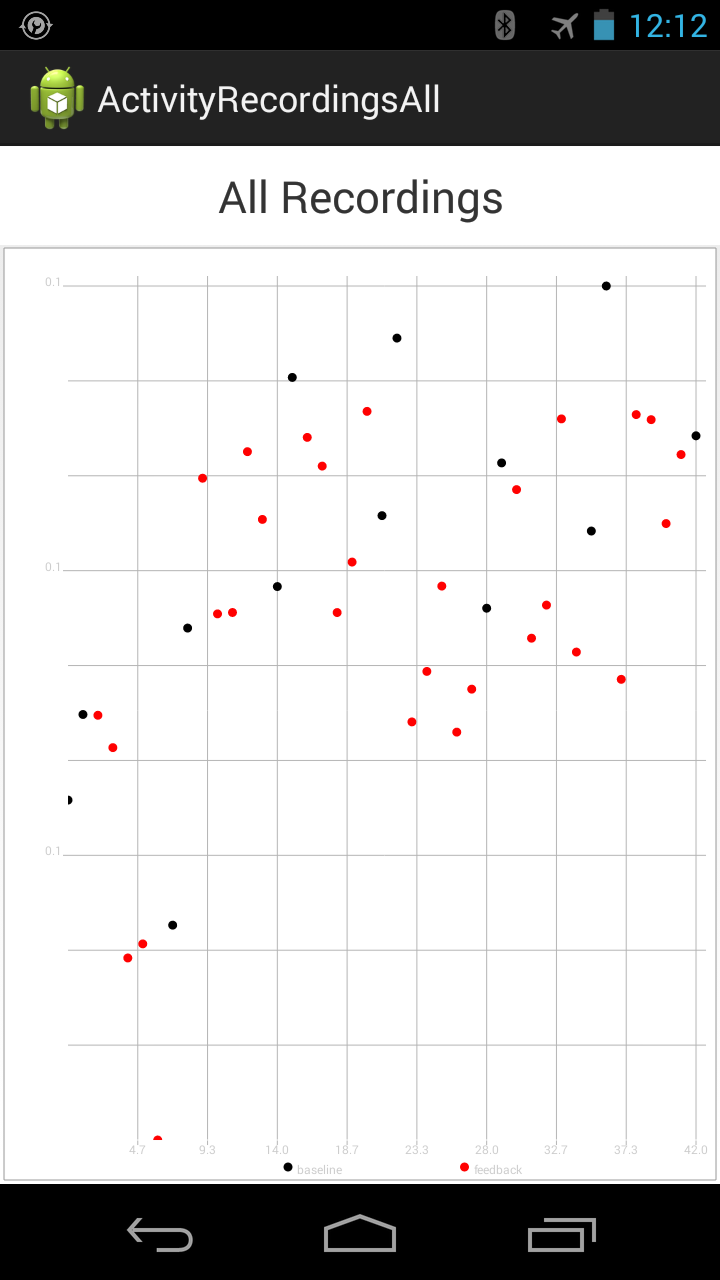
\includegraphics[width=0.800\linewidth]{early-prototype-screen-history.png}
\caption[History screen]{History screen: Baselines (black dots) and feedbacks (red dots).}\label{ch-design/index:fig-early-prototype-screen-history}\end{subfigure}
\caption[Screen shoots from early Android prototype]{Screenshots from the early prototype Android application using default Android UI components and manual interaction.}\phantomsection\label{ch-design/index:fig-early-prototype}

\end{figure}


We tested the prototype informally on ourselves, fellow students, friends and a
domain expert within BCI and HCI. From our testing three notions became clear.

First, we had to revisit our manual interaction and focus on \emph{accessibility}
regarding app functionality. It is not enough that the individual alpha peak can
be determined, baseline can be recorded, etc. when relying on the user to
calibrate (twice a day) and record baseline (once a day) - the user should not
even have to know about these concepts. We shifted our focus from \emph{availability}
to \emph{accessibility} in delegating the responsibility of taking appropriate
actions to the app by means of a proactive interaction described below in the
design of AlphaTrainer (Section {\hyperref[ch-design/index:ch-design-alphatrainer]{4.3}}).

Second, we gained several important insights about the 5
feedbacks. Interestingly, the bar height was perceived inversely proportional to
how it was designed. By design, a high bar represents high alpha from an alpha
performance metaphor ``more alpha is good''. However, some subjects experienced
the interface expressing state of mind from a ``low mind activity is good'' where
the obvious goal state of the feedback would be a low bar. We adopted the latter
metaphor when designing a new set of feedbacks for the next generation of
interfaces. However, the bar was generally experienced to be unpleasant for
other reasons - namely due to its radical shifts - why we excluded it from this
point. During the testing of the prototype, the idea of supporting other
modalities than sight was generated. This expanded the design space of the
feedbacks and led to the development of audio and tactile feedbacks. We ended
out with a set of 5 feedbacks: 2 visual (1 with history), 2 auditive (1 with
history) and 1 tactile. They are described below in the design of AlphaTrainer
(Section {\hyperref[ch-design/index:ch-design-alphatrainer]{4.3}}).

Third, we learned that the immediate impression of the app through the UI design
was an important part of the general experience of using the app. When
non-developers tried the prototype, they responded negatively to the standard
Android layout (see Figure \ref{ch-design/index:fig-early-prototype-app-screen-start})
which looks a lot more rough than they are used to from other apps.  We noted
that the general user is not able to abstract away from the graphical
layout. Since we wanted to deploy the app for real world usage, we wanted to
remove this obstacle of users distancing from the app due to its
layout. Assisted by a digital designer, we updated the graphical design.  The
result can be seen below in the final design of AlphaTrainer (Figure \ref{ch-design/index:fig-final-prototype-app-flow}).

Finally the last iteration of our prototype consisted of a test and analysis by
an interaction design expert and a pilot evaluation performed by our
selves. This had a set of concrete outcomes:
\begin{itemize}
\item {} 
The app should yield training performance immediately after a training has
been performed.

\item {} 
When headset connection fails, try to reconnect and/or show the user as
precise as possibly where the problem is.

\item {} 
History of training performance should be kept in the simple app design with a \emph{high
ink-to-information ratio} \cite{tufte_envisioning_1990}.

\end{itemize}

This ends our chronological journey through the design process. We now move
on to describe the AlphaTrainer system in its current state
- the version used in the user evaluation (Chapter {\hyperref[ch-evaluation/index:ch-evaluation]{6}}).


\section{AlphaTrainer}
\label{ch-design/index:ch-design-alphatrainer}\label{ch-design/index:alphatrainer}
This chapter concludes with a description of the resulting AlphaTrainer
prototype design. When the app is launched, the user is met by the home screen
(Figure \ref{ch-design/index:fig-final-prototype-app-flow-app-screen-start}). The home
screen contains a logo and the 3 buttons: ``Training'', ``History'' and
``Settings''. The logo is the Greek letter alpha, which we imagine the user of
AlphaTrainer (our personas) might recognize. The colors form a toned down blue
palette and in conjunction with the logo we aim at conveying that AlphaTrainer
is a serious tool.

\begin{figure}
\centering
\capstart
\begin{subfigure}[t]{0.30\linewidth}
\centering
\capstart

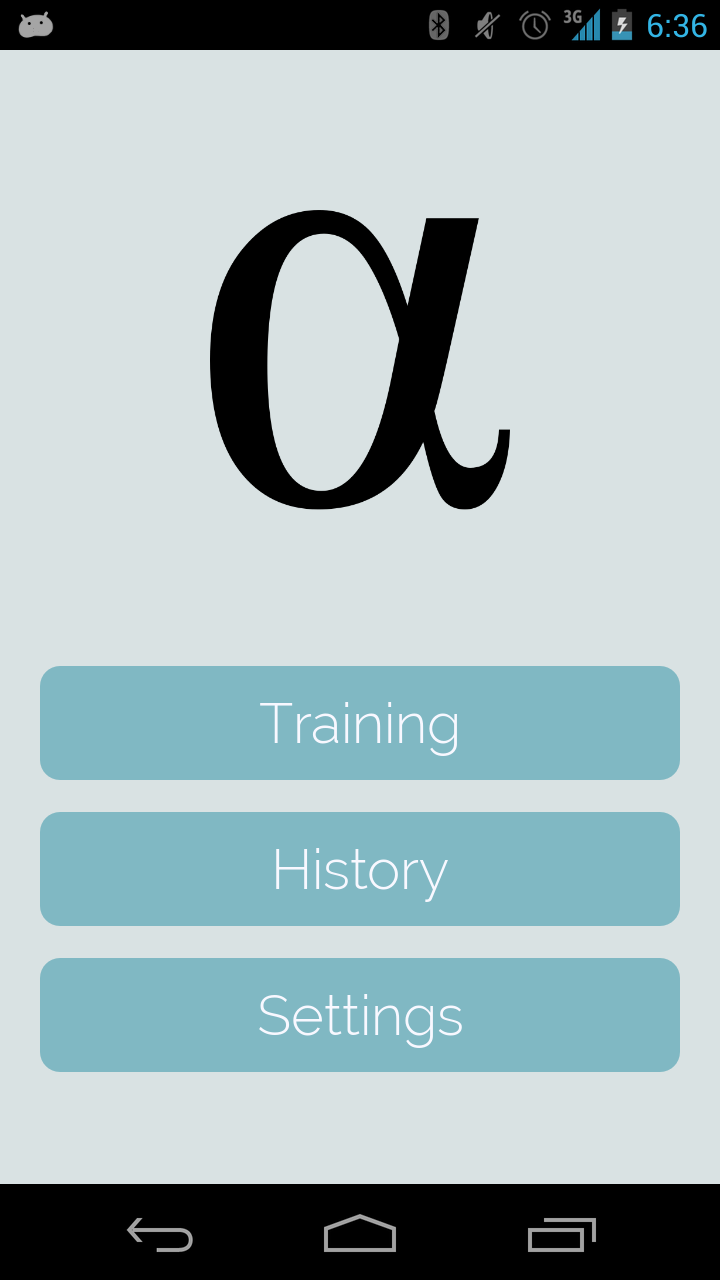
\includegraphics[width=0.800\linewidth]{final-prototype-start.png}
\caption[Start screen]{Start screen.}\label{ch-design/index:fig-final-prototype-app-flow-app-screen-start}\end{subfigure}
\begin{subfigure}[t]{0.30\linewidth}
\centering
\capstart

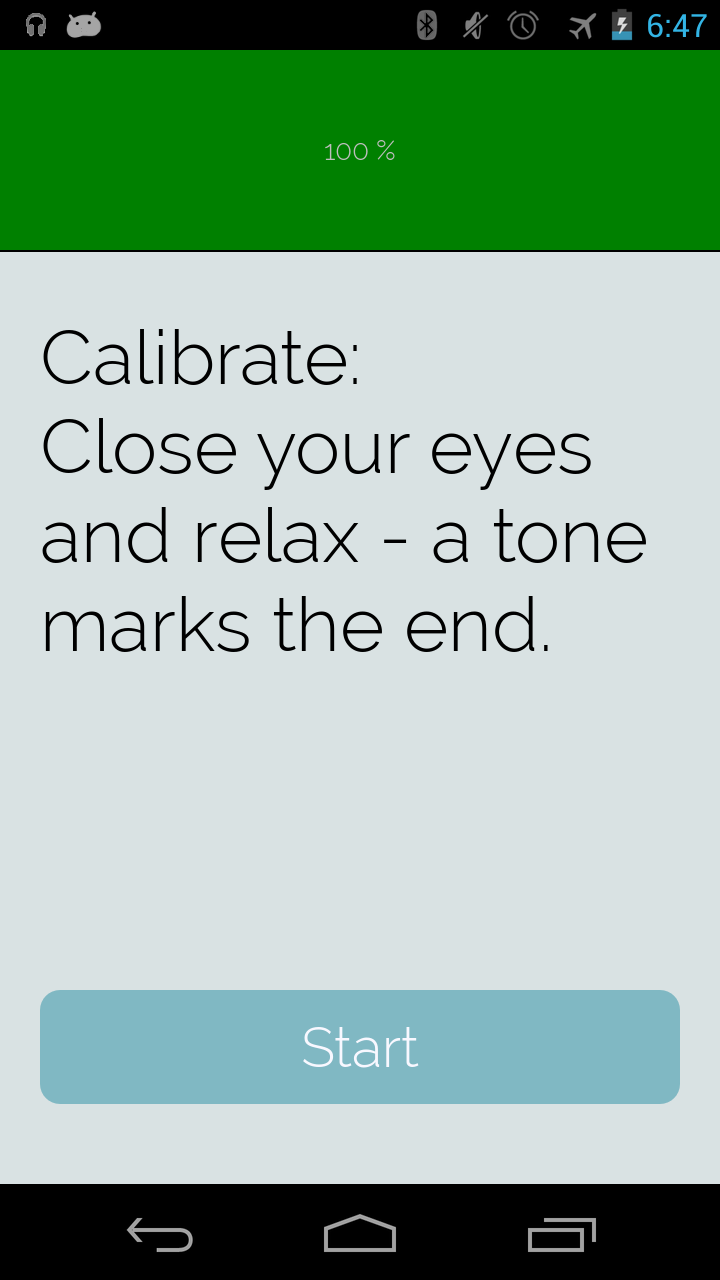
\includegraphics[width=0.800\linewidth]{final-prototype-calibrate-step-1.png}
\caption[Calibrate step 1]{Calibrate step 1.}\label{ch-design/index:fig-final-prototype-app-flow-calibrate-step-1}\end{subfigure}
\begin{subfigure}[t]{0.30\linewidth}
\centering
\capstart


\includegraphics[width=0.800\linewidth]{final-prototype-calibrate-step-2.png}
\caption[Calibrate step 2]{Calibrate step 2.}\label{ch-design/index:fig-final-prototype-app-flow-calibrate-step-2}\end{subfigure}
\begin{subfigure}[t]{0.30\linewidth}
\centering
\capstart

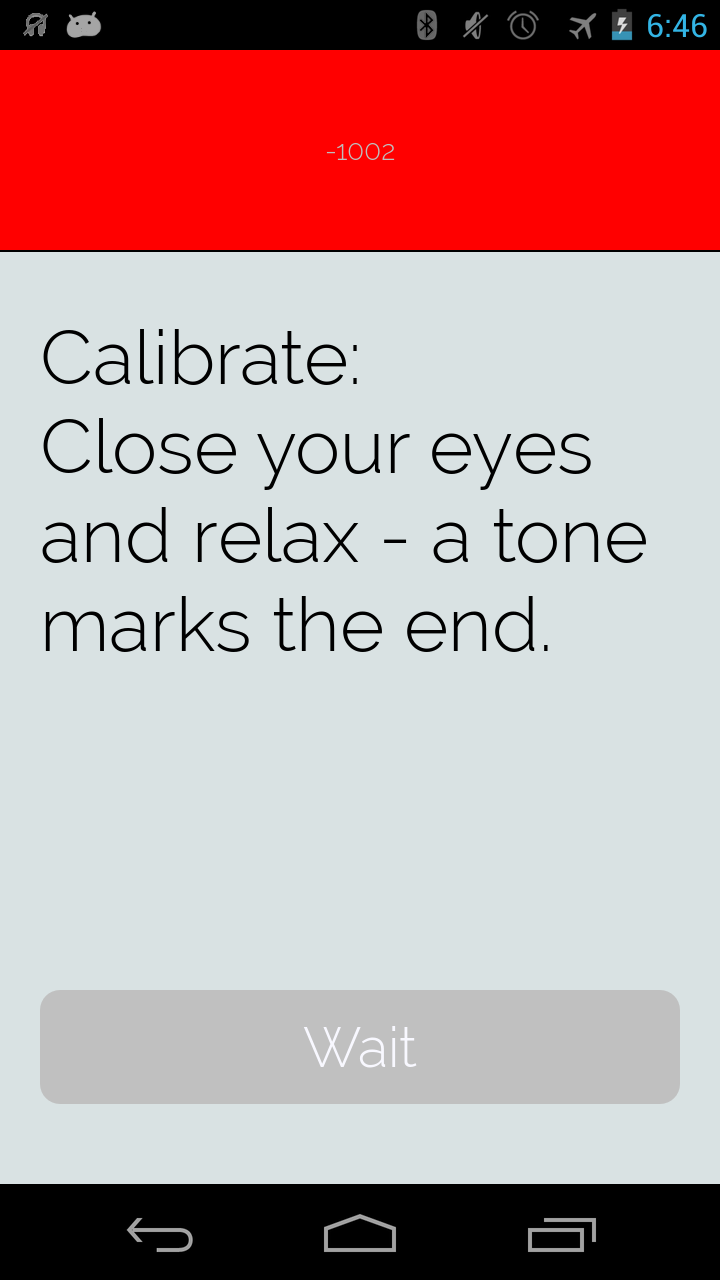
\includegraphics[width=0.800\linewidth]{final-prototype-calibrate-no-connect.png}
\caption[Not connected]{Not connected (headset).}\label{ch-design/index:fig-final-prototype-app-flow-calibrate-no-connect}\end{subfigure}
\begin{subfigure}[t]{0.30\linewidth}
\centering
\capstart

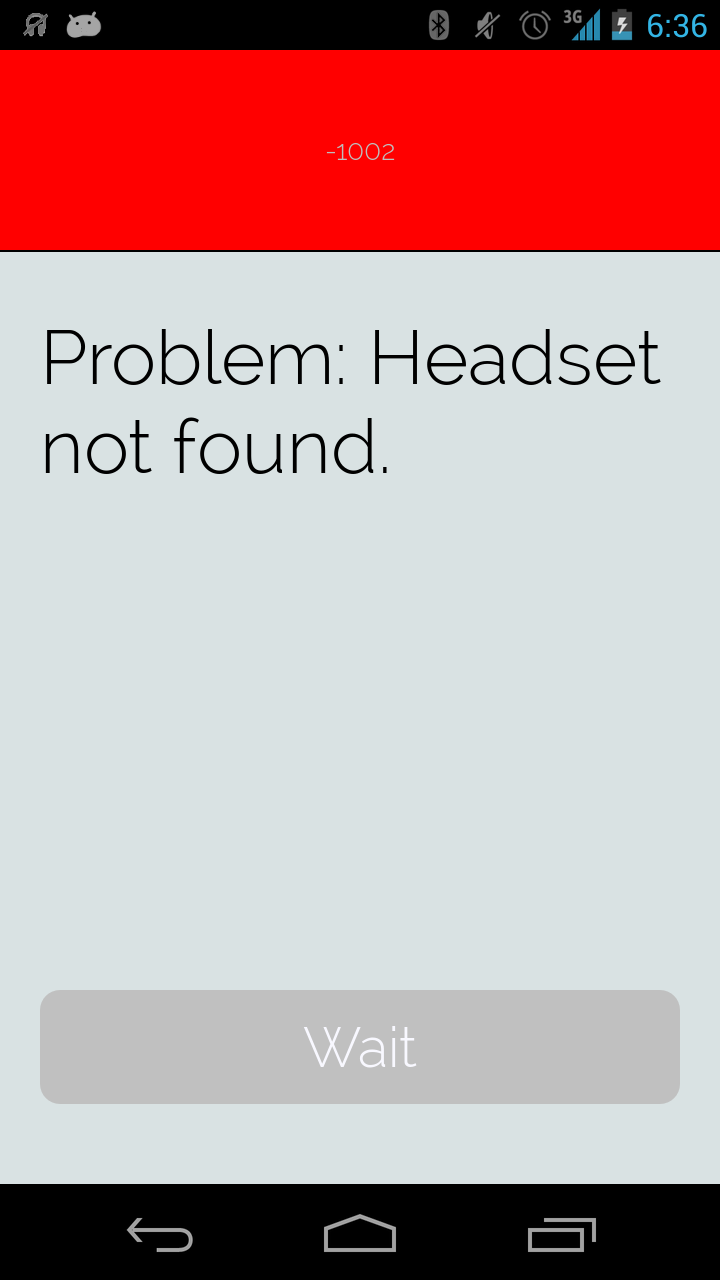
\includegraphics[width=0.800\linewidth]{final-prototype-no-headset-found.png}
\caption[No headset found]{No headset found.}\label{ch-design/index:fig-final-prototype-app-flow-no-headset-found}\end{subfigure}
\begin{subfigure}[t]{0.30\linewidth}
\centering
\capstart

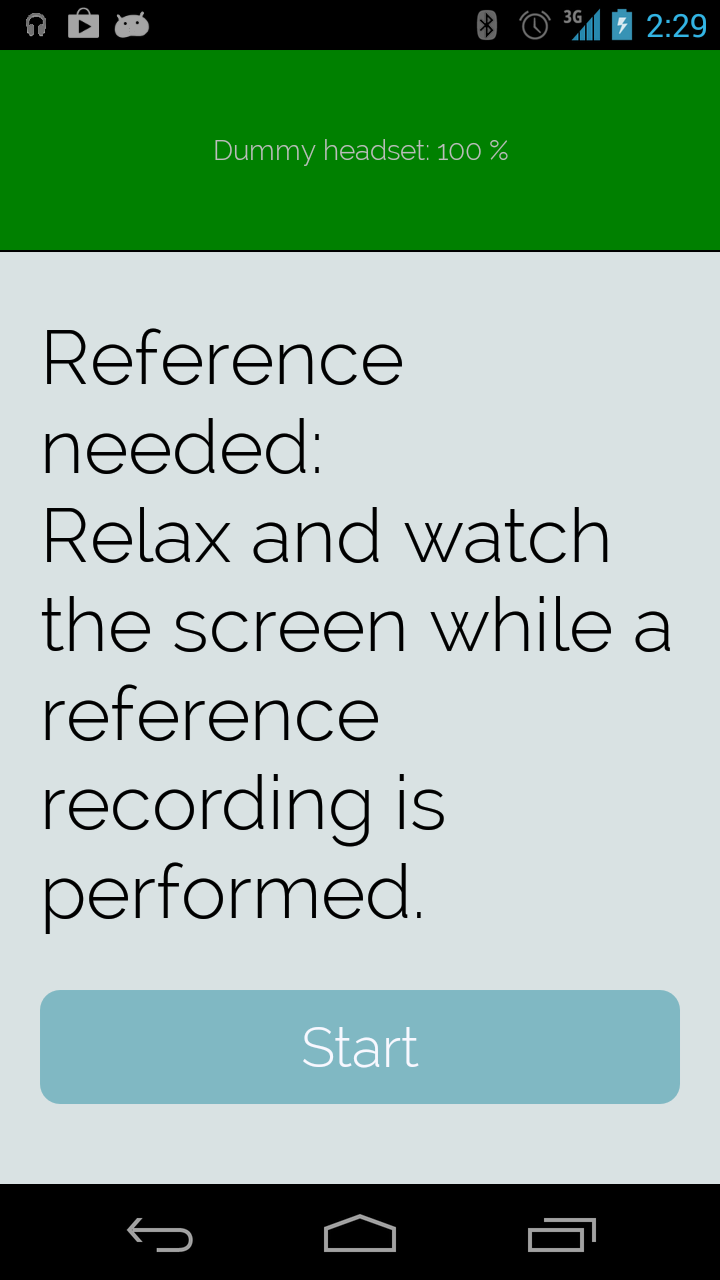
\includegraphics[width=0.800\linewidth]{final-prototype-reference.png}
\caption[Start reference recording]{Start ref. recording.}\label{ch-design/index:fig-final-prototype-app-flow-prototype-reference}\end{subfigure}
\begin{subfigure}[t]{0.30\linewidth}
\centering
\capstart

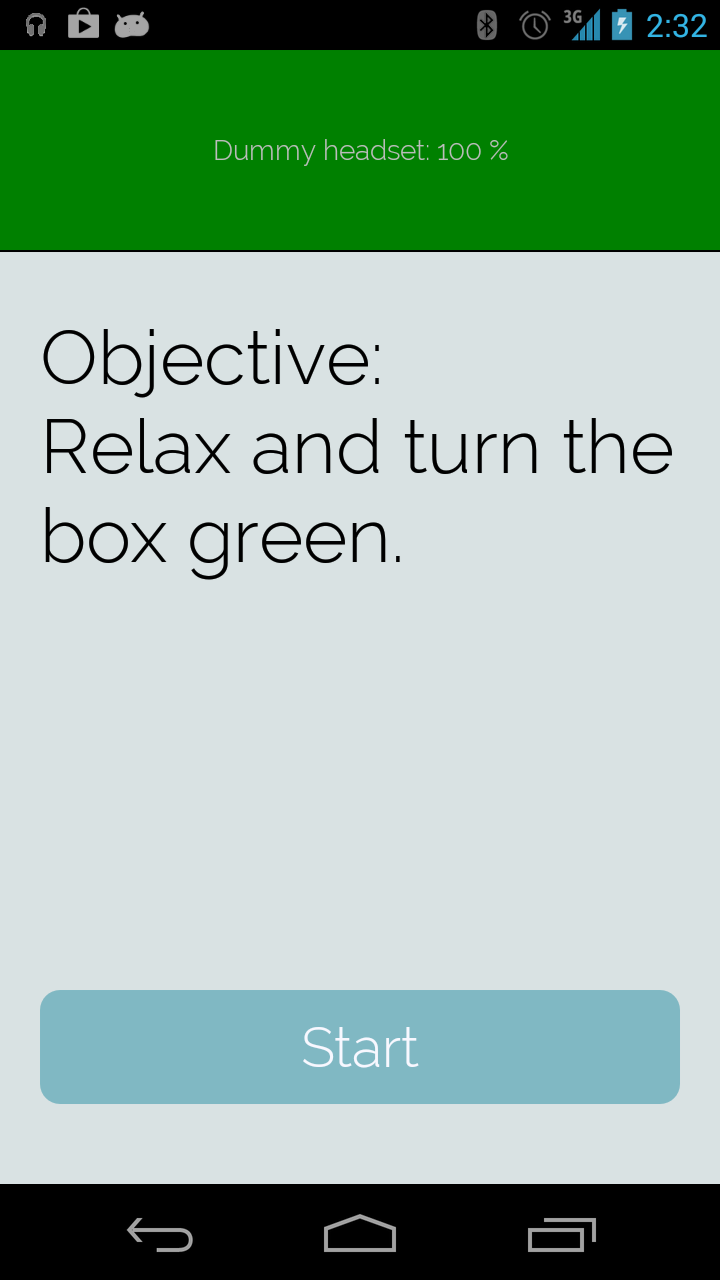
\includegraphics[width=0.800\linewidth]{final-prototype-training-start.png}
\caption[Training feedback instructions]{Training feedback instructions.}\label{ch-design/index:fig-final-prototype-app-flow-training-start}\end{subfigure}
\begin{subfigure}[t]{0.30\linewidth}
\centering
\capstart

\includegraphics[width=0.800\linewidth]{final-prototype-training-completed.png}
\caption[Training completed]{Training completed.}\label{ch-design/index:fig-final-prototype-app-flow-training-completed}\end{subfigure}
\begin{subfigure}[t]{0.30\linewidth}
\centering
\capstart

\includegraphics[width=0.800\linewidth]{final-prototype-history-overview.png}
\caption[Training history]{Training history (per day, week and month). Plots the last 10 feedback
recordings and the last 5 reference recordings.}\label{ch-design/index:fig-final-prototype-app-flow-training-history}\end{subfigure}
\caption[Screen shoots from the app flow of the final AlphaTrainer Android prototype]{Screen shoots from the app flow of the final AlphaTrainer Android
prototype.}\phantomsection\label{ch-design/index:fig-final-prototype-app-flow}

\end{figure}


When the user clicks ``Training'', the app takes on a proactive interaction. It
decides whether it needs to calibrate or to record a baseline before training
can be performed. The appropriate action is decided from these rules: (\emph{i}) if
calibration has not been performed within 8 hours, calibrate now; (\emph{ii}) if a
baseline has not been recorded today, record one now; finally (\emph{iii}) if the first two
criteria are met, the user is set to perform alpha feedback training.  The
headset connection status is shown in top of the screen both as a number (0 -
100\%) and by a color varying between red (0\%) over yellow (between 0\% and 100\%)
to green (100\%) (Figure \ref{ch-design/index:fig-final-prototype-app-flow-calibrate-step-1}). While connection is not
yet established, the button for starting the appropriate action is grayed
out. Should connection to the headset fail, the app will try its best to tell
the user what the problem is - for example in case the headset is turned off
(Figure \ref{ch-design/index:fig-final-prototype-app-flow-calibrate-no-connect}). The
app continuously tries to establish connection while being inside the ``Training''
area.

When ready to perform alpha feedback training, the app looks up which feedback
has been selected in the settings. The trainees objective is presented,
e.g. ``Relax and turn the box green'' in case of the box changing colors feedback
mentioned earlier. We ended up with 5 different feedbacks:
\begin{enumerate}
\item {} 
Box changing colors. This feedback contains no performance history (Figure \ref{ch-design/index:fig-final-prototype-feedback-1-box-colors}).

\item {} 
Circles that move according to alpha level from the logic that high alpha
amplitude (quiet state of mind) makes circle movement less. The circles are
affected by gravity which conveys the recent performance history - when alpha
level increases, it takes some time for the circles through the gravity to
reach a state in which they are still (Figure \ref{ch-design/index:fig-final-prototype-feedback-2-circles}).

\item {} 
Vibration feedback in which high alpha amplitude makes the phone vibrate
less. This feedback contains no performance history (Figure \ref{ch-design/index:fig-final-prototype-feedback-3-4-5}).

\item {} 
Tone generator in which the pitch of the tone represents the current alpha
level from the logic that high alpha amplitude (quiet state of mind) lowers
the pitch. This feedback contains no performance history (Figure \ref{ch-design/index:fig-final-prototype-feedback-3-4-5}).

\item {} 
Bell sounds appearing in which the number of bells represent the alpha level
from the logic that high alpha amplitude (quiet state of mind) makes a quiet
sound scape by having fewer bell sounds appear. When alpha level increase, it
takes some time for the bell sounds to disappear. Thereby the duration of the
bell sounds convey performance history (Figure \ref{ch-design/index:fig-final-prototype-feedback-3-4-5}).

\end{enumerate}

\begin{figure}
\centering
\capstart
\begin{subfigure}[t]{0.30\linewidth}
\centering
\capstart

\includegraphics[width=0.800\linewidth]{final-prototype-feedback-1-box-colors.png}
\caption[Feedback 1 with changing colors.]{Feedback 1 with changing colors objective is to turn the color
green (from red).}\label{ch-design/index:fig-final-prototype-feedback-1-box-colors}\end{subfigure}
\begin{subfigure}[t]{0.30\linewidth}
\centering
\capstart

\includegraphics[width=0.800\linewidth]{final-prototype-feedback-2-circles.png}
\caption[Moving circles.]{Feedback 2 with moving circles - objective less movements.}\label{ch-design/index:fig-final-prototype-feedback-2-circles}\end{subfigure}
\begin{subfigure}[t]{0.30\linewidth}
\centering
\capstart

\includegraphics[width=0.800\linewidth]{final-prototype-feedback-3-4-5.png}
\caption[Vibration, tone generator and bell sounds.]{Vibration, tone generator and bell sounds - they all share the
same screen instruction. Objectives make less vibration, lower
pitch of tone and less bells.}\label{ch-design/index:fig-final-prototype-feedback-3-4-5}\end{subfigure}
\caption[Screen shoots from the 5 feedbacks of the final Android prototype.]{Screen shoots from the 5 feedbacks of the final AlphaTrainer Android prototype.}\phantomsection\label{ch-design/index:fig-final-prototype-app-feedbacks}

\end{figure}


After a training has been performed, the user is immediately presented with a
number representing performance in percent. This number is calculated by comparing the
currently ended training session to the most recent training before that (Figure \ref{ch-design/index:fig-final-prototype-app-flow-training-completed}). The user can
then choose to train again by pushing the ``Try again'' button. This concludes the
``Training'' area of the app.

When the user selects ``History'' from the home screen, she is presented with a
simple history dashboard (Figure \ref{ch-design/index:fig-final-prototype-app-flow-training-history}). The training performance
of current day, current week and current month is presented in the top and
conveys the set of trainings compared to all training sessions performed. The
dashboard also has two simple graphs showing the recent training sessions and
the recent baseline recordings.

When the user selects ``Settings'' from the home screen, she is presented with a
conventional Android settings screen which enables her to choose among the 5
feedbacks described above.

We have now presented the AlphaTrainer and are now ready to cover the actual
implementations in detail in Chapter {\hyperref[ch-implementation/index:ch-implementation]{5}}.


\chapter{Implementation}
\label{ch-implementation/index:implementation}\label{ch-implementation/index:ch-implementation}\label{ch-implementation/index::doc}\begin{figure}[tbp]
\centering
\capstart

\includegraphics[width=1.000\linewidth]{alphatrainer-system-overview.png}
\caption[AlphaTrainer system overview]{Overview of the AlphaTrainer system components}\label{ch-implementation/index:fig-implementation-alphatrainer-system-overview}\end{figure}

AlphaTrainer is a system composed of several components. This chapter presents
each of their implementation. Figure \ref{ch-implementation/index:fig-implementation-alphatrainer-system-overview} gives an overview of
the different parts of AlphaTrainer and their relationship.


\section{Signal processing library}
\label{ch-implementation/index:ch-implementation-signal-processing-library}\label{ch-implementation/index:signal-processing-library}
Starting low level, we have implemented a small \emph{C++} library for processing raw
EEG data (Appendix {\hyperref[appendix_software:appendix-alphatrainer-signal-processing-library]{\emph{AlphaTrainer signal processing library}}}). It is based on the
open-source OpenCV 2 library \footnote{
\href{http://opencv.org}{http://opencv.org}
}.

OpenCV is primarily used for computer vision and contains methods for image
analysis and processing. OpenCV 2 has been rewritten from \emph{C} to \emph{C++} and is
optimized to handle numerical data like vectors or matrices of float values \cite{baggio_mastering_2012}. This is exactly what we need when
processing EEG data which at this level is represented as
arrays of float values.

The implementation of this library is based on the signal processing and EEG
data knowledge gained from the BCI Evaluation Chapter {\hyperref[ch-experiment/index:ch-experiment]{3}}. The strategies, algorithms and data cleaning are roughly
mirrored 1:1 in this library the main difference being that this library is
intended for real-time usage.

Implementing the signal processing in C++ was chosen due to its performance
advantages over Java in regard to numerical manipulation
\cite{ratabouil_android_2012}. This may seem overkill for the current
MindWave BCI configuration in which 512 data points are processed every second,
but it secures scalability for future headsets presumably increasing sample rate
and depth. For the same reason, we refrain from making the assumption that a headset
carries only one channel by letting the library support multichannel EEG data \footnote{
Multichannel EEG would require small adjustments in regard to the communicating with the library.
}.

The library can be called from the Java Virtual Machine (JVM) through the Java
Native Interface (JNI) \footnote{
\href{http://docs.oracle.com/javase/7/docs/technotes/guides/jni}{http://docs.oracle.com/javase/7/docs/technotes/guides/jni}.
} \cite{liu_android_2013}.

Usage of the library is defined in the \code{opencvbrainprocessor.h} interface:

\begin{Verbatim}[commandchars=\\\{\},numbers=left,firstnumber=1,stepnumber=1]
 \PYG{err}{\PYGZsh{}}\PYG{n}{include} \PYG{l+s}{\PYGZdq{}}\PYG{l+s}{opencv2/core/core.hpp}\PYG{l+s}{\PYGZdq{}}
 \PYG{err}{\PYGZsh{}}\PYG{n}{include} \PYG{l+s}{\PYGZdq{}}\PYG{l+s}{signalprocessingutil.h}\PYG{l+s}{\PYGZdq{}}

 \PYG{err}{\PYGZsh{}}\PYG{n}{ifndef} \PYG{n}{OPENCVBRAINPROCESSOR\PYGZus{}H\PYGZus{}}
 \PYG{err}{\PYGZsh{}}\PYG{n}{define} \PYG{n}{OPENCVBRAINPROCESSOR\PYGZus{}H\PYGZus{}}

 \PYG{k+kt}{float} \PYG{n}{getBrainProcessed}\PYG{p}{(}\PYG{k+kt}{float} \PYG{n}{eeg}\PYG{p}{[}\PYG{p}{]}\PYG{p}{,} \PYG{k+kt}{int} \PYG{n}{channels}\PYG{p}{,} \PYG{k+kt}{int} \PYG{n}{samples}\PYG{p}{,} \PYG{k+kt}{int} \PYG{n}{Fs}\PYG{p}{,}
                         \PYG{k+kt}{float} \PYG{n}{lowCutFq}\PYG{p}{,} \PYG{k+kt}{float} \PYG{n}{highCutFq}\PYG{p}{,} \PYG{k+kt}{float} \PYG{n}{alphaPeak}\PYG{p}{)}\PYG{p}{;}
 \PYG{k+kt}{float} \PYG{n+nf}{getAlphaPeak}\PYG{p}{(}\PYG{k+kt}{float} \PYG{n}{eeg}\PYG{p}{[}\PYG{p}{]}\PYG{p}{,} \PYG{k+kt}{int} \PYG{n}{channels}\PYG{p}{,} \PYG{k+kt}{int} \PYG{n}{samples}\PYG{p}{,} \PYG{k+kt}{int} \PYG{n}{Fs}\PYG{p}{)}\PYG{p}{;}
 \PYG{k+kt}{void} \PYG{n+nf}{getMinMax}\PYG{p}{(}\PYG{k+kt}{float} \PYG{n}{alphaLevels}\PYG{p}{[}\PYG{p}{]}\PYG{p}{,} \PYG{k+kt}{float}\PYG{o}{*} \PYG{n}{result}\PYG{p}{,} \PYG{k+kt}{int} \PYG{n}{alphaLevelsLength}\PYG{p}{,} \PYG{k+kt}{int} \PYG{n}{factor}\PYG{p}{)}\PYG{p}{;}
 \PYG{err}{\PYGZsh{}}\PYG{n}{endif} \PYG{c+cm}{/* OPENCVBRAINPROCESSOR\PYGZus{}H\PYGZus{} */}
\end{Verbatim}

This interface is implemented in \code{opencvbrainprocessor.cpp}. It contains three
methods which in combination make up our signal processing. We now briefly
explain the substance of each method.

The \code{getRelativeAlphaLevel()} method computes the relative alpha level taking
raw EEG data and the alpha peak frequency as input. The procedure consists of:
(\emph{i}) applying FFT to the EEG data; (\emph{ii}) then for each frequency bin of the
FFT output, the value is squared (to go from amplitude to power); finally
(\emph{iii}) return the relative alpha level which is calculated by dividing the
power of the alpha band (defined as 1 Hz to either side of the alpha peak
frequency) with the power of the total band (defined as the band between the
lowCutFq and highCutFq parameters).  During the BCI evaluation we had good
experiences with a low cut frequency of 5 Hz and a high cut frequency of 25
Hz ({\hyperref[ch-experiment/index:ch-experiment-processing]{3.2.2}}). These values are currently used by AlphaTrainer.

The \code{getAlphaPeak()} method computes which frequency has the highest occurring
amplitude within the alpha band (7 Hz - 13 Hz) taking raw EEG (recorded during
calibration) as input. The procedure is this: (\emph{i}) apply FFT to the EEG data;
(\emph{ii}) trim the resulting frequency domain down to the alpha band and; (\emph{iii}) find
the maximum amplitude and return the corresponding frequency.

Finally, the method \code{getMinMax()} computes how alpha levels should be mapped
to feedback states.  The resulting min and max values determine, for example,
the thresholds for the Box feedbacks red and green states. It takes an array of
relative alpha levels (from a baseline recording) as input. The procedure is to:
(\emph{i}) calculate mean and standard deviation of the input alpha levels; (\emph{ii})
set min/max values to mean +/- the standard deviation multiplied with a factor
(a method parameter); finally (\emph{iii}) if min \textless{} 0 it is replaced by the lowest
appearing value in the input data.

By design, this signal processing library is kept stateless. For example, it
receives the alpha peak frequency and sample rate for every alpha level
processing call. Keeping the processing module stateless simplifies the
integration with the app by allowing a low coupling. This will be elaborated in
the following section in which the library's user - the Android app - is
explained.


\section{Android app}
\label{ch-implementation/index:android-app}
Android is an open source operating system (OS) for mobile devices initiated by
Google. Our rationales for choosing
this platform includes that: (\emph{i}) fits well for prototyping; (\emph{ii}) has gained wide
adoption; and (\emph{iii}) has unrestricted deployment to end users through the Google Play store.

Android is a mature OS and is currently released in version 4.4. AlphaTrainer
requires Android 3.0 (API level 9) or later \footnote{
Main parts of the AlphaTrainer Android App work even from version
2.3 (API level 9) and up except of the Circle feedback covered within Section {\hyperref[ch-implementation/index:ch-implementation-feedback-ui-s]{5.2.6}}
which relies on browsers that implement Scalable Vector Graphics (SVG).
}.

An introduction to the Android programming model is out of scope - the interested reader
is referred to the comprehensive official documentation \footnote{
\href{http://developer.android.com/}{http://developer.android.com/}
}.
Instead, this section will focus on the overall architecture and the most important design patterns
used in the AlphaTrainer Android app implementation.


\subsection{Overview}
\label{ch-implementation/index:overview}\begin{figure}[tbp]
\centering
\capstart

\includegraphics[width=1.000\linewidth]{alphatrainer-android-app-architecture.png}
\caption[AlphaTrainer Android app architecture overview]{AlphaTrainer Android app architecture overview.}\label{ch-implementation/index:fig-implementation-alphatrainer-android-app-architecture}\end{figure}

An overview of the architecture is shown in Figure \ref{ch-implementation/index:fig-implementation-alphatrainer-android-app-architecture}. The diagram is
by no means exhaustive and the aim is to highlight the relationships between
BCIs (headsets), data processing, feedback views, application state and
persistent storage. This diagram will function as the reference throughout the
presentation of the Android app in the succeeding sections.

A main architectural goal of the implementation is a modular design which
enables replacement of the different components i.e. the headset, data processor
or the feedback view. How modularity is achieved will emerge during the
discussion of the individual components and their relations to other components.


\subsection{State management}
\label{ch-implementation/index:state-management}
We take a singleton approach \cite{bloch_effective_2008} to global app
state management. The singleton is implemented in the \code{App} class which
extends the Android framework \code{Application}. In short, the Android framework
guarantees that exactly one instance of the class is loaded at all times
throughout the lifetime of the application, which makes it safe to write a
\code{getInstance()} method \footnote{
\href{http://developer.android.com/reference/android/app/Application.html}{http://developer.android.com/reference/android/app/Application.html}
}.
Our application singleton is the center point for: (\emph{i}) reading user
preferences which takes place in the \code{SessionManager}; (\emph{ii}) reading and
writing from persistent storage which takes place in the data access object
\code{DAO}; and (\emph{iii}) managing headset connection which is takes place in
\code{HeadsetManager} as well as in the singleton itself.


\subsection{Headset}
\label{ch-implementation/index:headset}
To support future consumer BCIs such as the already announced Muse and Emotiv
INSIGHT (see Section {\hyperref[ch-background/index:ch-background-future-headsets]{2.2.4}}), we have put effort into
being as headset agnostic as
possible. Implementing the signal processing ourselves is one way of doing so
since this allows us not to rely on the signal processing abilities of a
specific BCIs SDK.

Another way to obtain headset agnosticism is by communicating with the specific
BCIs through a thin interface thus abstracting from the specific BCIs API by
wrapping it in an implementation of the \code{\textless{}\textless{}IHeadsetManagement\textgreater{}\textgreater{}} interface:

\begin{Verbatim}[commandchars=\\\{\},numbers=left,firstnumber=1,stepnumber=1]
 \PYG{k+kn}{package} \PYG{n}{dk}\PYG{o}{.}\PYG{n+na}{itu}\PYG{o}{.}\PYG{n+na}{alphatrainer}\PYG{o}{.}\PYG{n+na}{interfaces}\PYG{o}{;}
 \PYG{k+kd}{public} \PYG{k+kd}{interface} \PYG{n+nc}{IHeadset} \PYG{o}{\PYGZob{}}
     \PYG{k+kd}{public} \PYG{k+kt}{int} \PYG{n+nf}{getNrOfChannels}\PYG{o}{(}\PYG{o}{)}\PYG{o}{;}
     \PYG{k+kd}{public} \PYG{k+kt}{int} \PYG{n+nf}{getSampleRate}\PYG{o}{(}\PYG{o}{)}\PYG{o}{;}
     \PYG{k+kd}{public} \PYG{k+kt}{int} \PYG{n+nf}{getIcon}\PYG{o}{(}\PYG{o}{)}\PYG{o}{;}
 \PYG{o}{\PYGZcb{}}
 \PYG{k+kd}{public} \PYG{k+kd}{interface} \PYG{n+nc}{IHeadsetManagement} \PYG{k+kd}{extends} \PYG{n}{IHeadset} \PYG{o}{\PYGZob{}}
     \PYG{k+kd}{public} \PYG{k+kt}{void} \PYG{n+nf}{startDataStream}\PYG{o}{(}\PYG{o}{)}\PYG{o}{;}
     \PYG{k+kd}{public} \PYG{k+kt}{void} \PYG{n+nf}{stopDataStream}\PYG{o}{(}\PYG{o}{)}\PYG{o}{;}
 \PYG{o}{\PYGZcb{}}
\end{Verbatim}

Only the \code{HeadsetManager} uses the \code{\textless{}\textless{}IHeadsetManagement\textgreater{}\textgreater{}} interface. All other
communication with the headset goes through the methods defined by \code{\textless{}\textless{}IHeadset\textgreater{}\textgreater{}}
through which meta-data about the headset can be accessed.

AlphaTrainer currently contains two \code{\textless{}\textless{}IHeadsetManagement\textgreater{}\textgreater{}} implementations:
\code{DummyHeadset} and \code{MindWaveMobile} - both in the
\code{dk.itu.alphatrainer.headset} package. The \code{DummyHeadset} is used for
development and testing and it outputs a random signal.  The \code{MindWaveMobile}
implements and uses the \emph{ThinkGear} API \footnote{
\href{http://developer.neurosky.com/docs/doku.php?id=thinkgear\_connector\_tgc}{http://developer.neurosky.com/docs/doku.php?id=thinkgear\_connector\_tgc}
} bundled with the MindWave Mobile headset
(Section {\hyperref[ch-background/index:ch-background-mindwave]{2.2.2}}). Concrete communication with the
MindWave headset goes through the \code{TGDevice} class. An example of the
\code{\textless{}\textless{}IHeadsetManagement\textgreater{}\textgreater{}} interface implementation is shown below:

\begin{Verbatim}[commandchars=\\\{\},numbers=left,firstnumber=1,stepnumber=1]
 \PYG{k+kn}{package} \PYG{n}{dk}\PYG{o}{.}\PYG{n+na}{itu}\PYG{o}{.}\PYG{n+na}{alphatrainer}\PYG{o}{.}\PYG{n+na}{headset}\PYG{o}{;}
 \PYG{o}{.}\PYG{o}{.}\PYG{o}{.}
 \PYG{k+kn}{import} \PYG{n+nn}{com.neurosky.thinkgear.TGDevice}\PYG{o}{;}
 \PYG{k+kd}{public} \PYG{k+kd}{class} \PYG{n+nc}{MindWaveMobile} \PYG{k+kd}{implements} \PYG{n}{IHeadsetManagement} \PYG{o}{\PYGZob{}}
     \PYG{k+kd}{private} \PYG{n}{BluetoothAdapter} \PYG{n}{bluetoothAdapter}\PYG{o}{;}
     \PYG{k+kd}{private} \PYG{n}{TGDevice} \PYG{n}{tgDevice}\PYG{o}{;}
     \PYG{o}{.}\PYG{o}{.}\PYG{o}{.}
     \PYG{k+kd}{public} \PYG{n+nf}{MindWaveMobile}\PYG{o}{(}\PYG{n}{IHeadsetListener} \PYG{n}{listener}\PYG{o}{)} \PYG{o}{\PYGZob{}}
         \PYG{k}{this}\PYG{o}{.}\PYG{n+na}{listener} \PYG{o}{=} \PYG{n}{listener}\PYG{o}{;}
     \PYG{o}{\PYGZcb{}}
     \PYG{o}{.}\PYG{o}{.}\PYG{o}{.}
     \PYG{n+nd}{@Override}
     \PYG{k+kd}{public} \PYG{k+kt}{void} \PYG{n+nf}{startDataStream}\PYG{o}{(}\PYG{o}{)} \PYG{o}{\PYGZob{}}
         \PYG{o}{.}\PYG{o}{.}\PYG{o}{.}
         \PYG{n}{bluetoothAdapter} \PYG{o}{=} \PYG{n}{BluetoothAdapter}\PYG{o}{.}\PYG{n+na}{getDefaultAdapter}\PYG{o}{(}\PYG{o}{)}\PYG{o}{;}
         \PYG{o}{.}\PYG{o}{.}\PYG{o}{.}
         \PYG{k}{if} \PYG{o}{(}\PYG{n}{bluetoothAdapter} \PYG{o}{!}\PYG{o}{=} \PYG{k+kc}{null}\PYG{o}{)} \PYG{o}{\PYGZob{}}
             \PYG{n}{tgDevice} \PYG{o}{=} \PYG{k}{new} \PYG{n}{TGDevice}\PYG{o}{(}\PYG{n}{bluetoothAdapter}\PYG{o}{,} \PYG{n}{handler}\PYG{o}{)}\PYG{o}{;}
         \PYG{o}{\PYGZcb{}}
         \PYG{o}{.}\PYG{o}{.}\PYG{o}{.}
         \PYG{n}{tgDevice}\PYG{o}{.}\PYG{n+na}{connect}\PYG{o}{(}\PYG{k+kc}{true}\PYG{o}{)}\PYG{o}{;}
         \PYG{o}{.}\PYG{o}{.}\PYG{o}{.}
     \PYG{o}{\PYGZcb{}}
     \PYG{n+nd}{@Override}
     \PYG{k+kd}{public} \PYG{k+kt}{void} \PYG{n+nf}{stopDataStream}\PYG{o}{(}\PYG{o}{)} \PYG{o}{\PYGZob{}}
         \PYG{n}{tgDevice}\PYG{o}{.}\PYG{n+na}{stop}\PYG{o}{(}\PYG{o}{)}\PYG{o}{;}
         \PYG{n}{tgDevice}\PYG{o}{.}\PYG{n+na}{close}\PYG{o}{(}\PYG{o}{)}\PYG{o}{;}
     \PYG{o}{\PYGZcb{}}
     \PYG{o}{.}\PYG{o}{.}\PYG{o}{.}
\end{Verbatim}

Distribution of data from the headset is implemented in a publish subscribe pattern.
In order to receive data from the headset, a class must implement the \code{\textless{}\textless{}IHeadsetDataListener\textgreater{}\textgreater{}}
interface:

\begin{Verbatim}[commandchars=\\\{\},numbers=left,firstnumber=1,stepnumber=1]
\PYG{k+kn}{package} \PYG{n}{dk}\PYG{o}{.}\PYG{n+na}{itu}\PYG{o}{.}\PYG{n+na}{alphatrainer}\PYG{o}{.}\PYG{n+na}{interfaces}\PYG{o}{;}
    \PYG{k+kd}{public} \PYG{k+kd}{interface} \PYG{n+nc}{IHeadsetDataListener} \PYG{o}{\PYGZob{}}
    \PYG{k+kd}{public} \PYG{k+kt}{void} \PYG{n+nf}{onDataPacket}\PYG{o}{(}\PYG{k+kt}{int} \PYG{n}{channels}\PYG{o}{,} \PYG{k+kt}{float}\PYG{o}{[}\PYG{o}{]}\PYG{o}{[}\PYG{o}{]} \PYG{n}{data}\PYG{o}{)}\PYG{o}{;}
\PYG{o}{\PYGZcb{}}
\end{Verbatim}

Whenever a headset receives data, it calls its \code{\textless{}\textless{}IHeadsetListener\textgreater{}\textgreater{}} with the data formatted
in the form of an array of float arrays each representing an EEG channel. This will
always be the \code{HeadsetManager} which is the only class implementing the \code{\textless{}\textless{}IHeadsetListener\textgreater{}\textgreater{}}
interface which generalizes the \code{\textless{}\textless{}IHeadsetDataListener\textgreater{}\textgreater{}} and \code{\textless{}\textless{}IHeadsetConnectionStatusListener\textgreater{}\textgreater{}}
interfaces. The HeadsetManager then distributes the data to each of its registered
\code{\textless{}\textless{}IHeadsetDataListener\textgreater{}\textgreater{}} thus carrying out the publisher act. Below we see an example
showing how the private class \code{CalibrationDataHandler} within \code{ActivityCalibrate}
first registers itself for receiving EEG data (l. 7) and later calls the headset for
meta-data (l. 8-9).

\begin{Verbatim}[commandchars=\\\{\},numbers=left,firstnumber=1,stepnumber=1]
 \PYG{k+kn}{package} \PYG{n}{dk}\PYG{o}{.}\PYG{n+na}{itu}\PYG{o}{.}\PYG{n+na}{alphatrainer}\PYG{o}{.}\PYG{n+na}{calibration}\PYG{o}{;}
 \PYG{o}{.}\PYG{o}{.}\PYG{o}{.}
 \PYG{k+kd}{private} \PYG{k+kd}{class} \PYG{n+nc}{CalibrationDataHandler} \PYG{k+kd}{implements} \PYG{n}{IHeadsetDataListener} \PYG{o}{\PYGZob{}}
     \PYG{o}{.}\PYG{o}{.}\PYG{o}{.}
     \PYG{k+kd}{public} \PYG{n+nf}{CalibrationDataHandler}\PYG{o}{(}\PYG{n}{ActivityCalibrate} \PYG{n}{parent}\PYG{o}{)} \PYG{o}{\PYGZob{}}
         \PYG{k}{this}\PYG{o}{.}\PYG{n+na}{parent} \PYG{o}{=} \PYG{n}{parent}\PYG{o}{;}
         \PYG{n}{App}\PYG{o}{.}\PYG{n+na}{getInstance}\PYG{o}{(}\PYG{o}{)}\PYG{o}{.}\PYG{n+na}{getHeadsetManager}\PYG{o}{(}\PYG{o}{)}\PYG{o}{.}\PYG{n+na}{subscribeData}\PYG{o}{(}\PYG{k}{this}\PYG{o}{)}\PYG{o}{;}
         \PYG{n}{Fs} \PYG{o}{=} \PYG{n}{App}\PYG{o}{.}\PYG{n+na}{getInstance}\PYG{o}{(}\PYG{o}{)}\PYG{o}{.}\PYG{n+na}{getHeadsetManager}\PYG{o}{(}\PYG{o}{)}\PYG{o}{.}\PYG{n+na}{getHeadset}\PYG{o}{(}\PYG{o}{)}\PYG{o}{.}\PYG{n+na}{getSampleRate}\PYG{o}{(}\PYG{o}{)}\PYG{o}{;}
         \PYG{k+kt}{int} \PYG{n}{numberOfChannels} \PYG{o}{=} \PYG{n}{App}\PYG{o}{.}\PYG{n+na}{getInstance}\PYG{o}{(}\PYG{o}{)}\PYG{o}{.}\PYG{n+na}{getHeadsetManager}\PYG{o}{(}\PYG{o}{)}\PYG{o}{.}\PYG{n+na}{getHeadset}\PYG{o}{(}\PYG{o}{)}\PYG{o}{.}\PYG{n+na}{getNrOfChannels}\PYG{o}{(}\PYG{o}{)}\PYG{o}{;}
         \PYG{o}{.}\PYG{o}{.}\PYG{o}{.}
\end{Verbatim}

The distribution of connection status updates is similarly implemented in a
publish subscribe pattern using the \code{\textless{}\textless{}IHeadsetConnectionStatusListener\textgreater{}\textgreater{}}
interface.

Since the headset can be changed by the user through a settings entry and we
generally want the app to depend as little as possible on the concrete
headset implementations, we have implemented the factory pattern. Specifically,
the headsets are instantiated by the \code{HeadsetFactory} in the package
\code{dk.itu.alphatrainer.factories} which is responsible for instantiating a concrete
headset appropriate for the current headset settings entry.


\subsection{Signal processing}
\label{ch-implementation/index:signal-processing}
The implementation of the signal processing takes the same approach as was
taken with the
headsets to achieve modularity.
Again, the communication goes through a thin interface which allows for
easy replacement of the signal processing module.

\begin{Verbatim}[commandchars=\\\{\},numbers=left,firstnumber=1,stepnumber=1]
 \PYG{k+kn}{package} \PYG{n}{dk}\PYG{o}{.}\PYG{n+na}{itu}\PYG{o}{.}\PYG{n+na}{alphatrainer}\PYG{o}{.}\PYG{n+na}{interfaces}\PYG{o}{;}
 \PYG{k+kn}{import} \PYG{n+nn}{dk.itu.alphatrainer.model.AlphaMinMax}\PYG{o}{;}
 \PYG{k+kd}{public} \PYG{k+kd}{interface} \PYG{n+nc}{ISignalProcessor} \PYG{o}{\PYGZob{}}
     \PYG{k+kd}{public} \PYG{k+kt}{void} \PYG{n+nf}{getBandPower}\PYG{o}{(}\PYG{k+kt}{float}\PYG{o}{[}\PYG{o}{]}\PYG{o}{[}\PYG{o}{]} \PYG{n}{data}\PYG{o}{,} \PYG{k+kt}{int} \PYG{n}{Fs}\PYG{o}{,} \PYG{k+kt}{float} \PYG{n}{alphaPeak}\PYG{o}{)}\PYG{o}{;}
     \PYG{k+kd}{public} \PYG{k+kt}{float} \PYG{n+nf}{getAlphaPeak}\PYG{o}{(}\PYG{k+kt}{float}\PYG{o}{[}\PYG{o}{]}\PYG{o}{[}\PYG{o}{]} \PYG{n}{data}\PYG{o}{,} \PYG{k+kt}{int} \PYG{n}{Fs}\PYG{o}{)}\PYG{o}{;}
     \PYG{k+kd}{public} \PYG{n}{AlphaMinMax} \PYG{n+nf}{getMinMax}\PYG{o}{(}\PYG{k+kt}{float}\PYG{o}{[}\PYG{o}{]} \PYG{n}{alphaPowers}\PYG{o}{)}\PYG{o}{;}
 \PYG{o}{\PYGZcb{}}
 \PYG{k+kd}{public} \PYG{k+kd}{interface} \PYG{n+nc}{ISignalProcessingListener} \PYG{o}{\PYGZob{}}
     \PYG{k+kd}{public} \PYG{k+kt}{void} \PYG{n+nf}{onSignalProcessed}\PYG{o}{(}\PYG{k+kt}{float} \PYG{n}{bandPower}\PYG{o}{)}\PYG{o}{;}
 \PYG{o}{\PYGZcb{}}
\end{Verbatim}

\code{\textless{}\textless{}ISignalProcessor\textgreater{}\textgreater{}} is currently implemented by \code{DummySignalProcessor} and
\code{OpenCVSignalProcessor} found in the \code{dk.itu.alphatrainer.signalprocessing}
package. The \code{DummySignalProcessor} is for development and testing, and it
simply outputs dummy values. \code{OpenCVSignalProcessor} encapsulates the OpenCV
based library described in Section {\hyperref[ch-implementation/index:ch-implementation-signal-processing-library]{5.1}}. In the example below,
important lines of
\code{OpenCVSignalProcessor} are shown in which it receives its listener
in the constructor and
declares its usage of the C++ library (Section {\hyperref[ch-implementation/index:ch-implementation-signal-processing-library]{5.1}}) through the \code{native}
keyword:

\begin{Verbatim}[commandchars=\\\{\},numbers=left,firstnumber=1,stepnumber=1]
 \PYG{k+kn}{package} \PYG{n}{dk}\PYG{o}{.}\PYG{n+na}{itu}\PYG{o}{.}\PYG{n+na}{alphatrainer}\PYG{o}{.}\PYG{n+na}{signalprocessing}\PYG{o}{;}
 \PYG{o}{.}\PYG{o}{.}\PYG{o}{.}
 \PYG{k+kd}{public} \PYG{k+kd}{class} \PYG{n+nc}{OpenCVSignalProcessor} \PYG{k+kd}{implements} \PYG{n}{ISignalProcessor} \PYG{o}{\PYGZob{}}
     \PYG{o}{.}\PYG{o}{.}\PYG{o}{.}
     \PYG{k+kd}{private} \PYG{n}{ISignalProcessingListener} \PYG{n}{listener}\PYG{o}{;}
     \PYG{k+kd}{public} \PYG{n+nf}{OpenCVSignalProcessor}\PYG{o}{(}\PYG{n}{ISignalProcessingListener} \PYG{n}{listener}\PYG{o}{)} \PYG{o}{\PYGZob{}}
         \PYG{k}{this}\PYG{o}{.}\PYG{n+na}{listener} \PYG{o}{=} \PYG{n}{listener}\PYG{o}{;}
     \PYG{o}{\PYGZcb{}}
     \PYG{o}{.}\PYG{o}{.}\PYG{o}{.}
     \PYG{k+kd}{public} \PYG{k+kd}{native} \PYG{k+kt}{float} \PYG{n+nf}{getRelativeAlphaLevel}\PYG{o}{(}\PYG{k+kt}{float}\PYG{o}{[}\PYG{o}{]} \PYG{n}{eeg}\PYG{o}{,} \PYG{k+kt}{int} \PYG{n}{samples}\PYG{o}{,} \PYG{k+kt}{int} \PYG{n}{Fs}\PYG{o}{,} \PYG{k+kt}{float} \PYG{n}{alphaPeak}\PYG{o}{)}\PYG{o}{;}
     \PYG{o}{.}\PYG{o}{.}\PYG{o}{.}
\end{Verbatim}


\subsection{Data flow}
\label{ch-implementation/index:data-flow}
This section describes the data flow and call hierarchy involved from
the point where the BCI receives raw EEG data up till the point where the
feedback view is called with a processed and normalized alpha level.

As can be seen in the app overview diagram Figure \ref{ch-implementation/index:fig-implementation-alphatrainer-android-app-architecture}, the
\code{FeedbackLogic} class connects the raw EEG data, the signal processing and the
feedback UI. Figure \ref{ch-implementation/index:fig-flow-diagram-feedback} shows a
flow diagram of the calls involved from raw EEG is received to the feedback UI
is called. Notice how all calls between the classes are interface method calls
and would be exactly the same for other combinations of headset, processor and
feedback UI.

The diagram also shows our usage of the publish subscribe pattern in that the
\code{HeadsetManager} distributes the received EEG data to all listeners
registered for receiving data.
\begin{figure}[tbp]
\centering
\capstart

\includegraphics[width=1.000\linewidth]{flow-diagram-feedback.png}
\caption[Flow from EEG to feedback]{Flow of data from from headset receiving raw EEG to the feedback is drawn.}\label{ch-implementation/index:fig-flow-diagram-feedback}\end{figure}


\subsection{Feedback user interfaces}
\label{ch-implementation/index:ch-implementation-feedback-ui-s}\label{ch-implementation/index:feedback-user-interfaces}
A feedback UI is generalized in a simple interface:

\begin{Verbatim}[commandchars=\\\{\},numbers=left,firstnumber=1,stepnumber=1]
 \PYG{k+kn}{package} \PYG{n}{dk}\PYG{o}{.}\PYG{n+na}{itu}\PYG{o}{.}\PYG{n+na}{alphatrainer}\PYG{o}{.}\PYG{n+na}{interfaces}\PYG{o}{;}
 \PYG{k+kd}{public} \PYG{k+kd}{interface} \PYG{n+nc}{IFeedbackUi} \PYG{o}{\PYGZob{}}
     \PYG{k+kd}{public} \PYG{k+kt}{void} \PYG{n+nf}{drawFeedback}\PYG{o}{(}\PYG{k+kt}{int} \PYG{n}{i}\PYG{o}{)}\PYG{o}{;}
     \PYG{k+kd}{public} \PYG{k+kt}{void} \PYG{n+nf}{stop}\PYG{o}{(}\PYG{o}{)}\PYG{o}{;}
 \PYG{o}{\PYGZcb{}}
\end{Verbatim}

The \code{drawFeedback()} method takes a normalized alpha level from 0 to 100 and
transforms this number into a visible, auditive or tactile feedback to the user.
We have currently implemented 5 different feedback UIs found in the
\code{dk.itu.alphatrainer.ui.feedback} package - reference the Design Chapter {\hyperref[ch-design/index:ch-design]{4}} for a visual and conceptual explanation of each feedback
Figure \ref{ch-design/index:fig-final-prototype-app-feedbacks}. The feedback package
consists of:
\begin{enumerate}
\item {} 
\emph{Box} is implemented in the \code{FeedbackBox} class. It uses build-in Android
animation features to make the transitions from red to green depending on the
normalized alpha level.

\item {} 
\emph{Circles} is implemented in the \code{FeedbackCollision} class. It uses an
Android WebView and the circles are based on the open-source visualization
Javascript library \emph{d3.js} \footnote{
\emph{d3.js} is written in Javascript and it heavily relies on SVG - \href{http://d3js.org}{http://d3js.org}
}. The WebView
loads the Javascript and HTML/CSS from the Android specific \emph{assets} folder
within the AlphaTrainer Android app.
On receiving a normalized alpha level, \code{FeedbackCollision} dispatches it
to the WebView which handles the feedback actuation in a Javascript method.

\item {} 
\emph{Vibration} is implemented in the \code{FeedbackVibrate} class and utilizes the
Android system service architecture through which the vibration of the phone
can be accessed.

\item {} 
\emph{Tone} is implemented in the \code{FeedbackAudioSynth} class. It uses the build
in Android audio library in conjunction with pure Java to crate a small
synthesizer.

\item {} 
\emph{Bells} is implemented in the \code{FeedbackAudioClips} class. It uses another
build in Android audio library able to load and play sound clips from files.

\end{enumerate}

Similar to the headsets, the feedbacks can be changed by the user through a setting.
For the same reason, we also use the factory pattern to
instantiate a concrete feedback UI class. This responsibility is delegated
to the \code{FeedbackUiFactory} which read the user setting and instantiate the
appropriate feedback.


\subsection{Models and persistent storage}
\label{ch-implementation/index:ch-implementation-models-persistent-storage}\label{ch-implementation/index:models-and-persistent-storage}
We have benefited of the built in SQLite \footnote{
\href{http://www.sqlite.org/}{http://www.sqlite.org/}
} database
within the Android framework. All training data such as alpha peak frequencies and
the relative alpha levels are timestamped and persistently stored in the SQLite database
from where they can be
queried with SQL \footnote{
\href{http://en.wikipedia.org/wiki/SQL}{http://en.wikipedia.org/wiki/SQL}
}. The raw EEG data is currently
stored in plain text files on the mobile device's SD card.

All concrete database communication takes place in the \code{DAO} class from the
\code{dk.itu.alphatrainer.datastorage} package. This encapsulation
represents another typical design-pattern with Java and Android \cite{wei_android_2012}.

We have modeled a training and a processed alpha level respectively as
\code{Recording} and \code{AlphaLevel} classes within the \code{dk.itu.alphatrainer.model} package.
Below a snippet from the \code{AlphaLevel} class:

\begin{Verbatim}[commandchars=\\\{\},numbers=left,firstnumber=1,stepnumber=1]
 \PYG{k+kn}{package} \PYG{n}{dk}\PYG{o}{.}\PYG{n+na}{itu}\PYG{o}{.}\PYG{n+na}{alphatrainer}\PYG{o}{.}\PYG{n+na}{model}\PYG{o}{;}
 \PYG{o}{.}\PYG{o}{.}\PYG{o}{.}
 \PYG{k+kn}{import} \PYG{n+nn}{com.google.gson.annotations.Expose}\PYG{o}{;}
 \PYG{k+kn}{import} \PYG{n+nn}{com.google.gson.annotations.SerializedName}\PYG{o}{;}
 \PYG{o}{.}\PYG{o}{.}\PYG{o}{.}
 \PYG{k+kd}{public} \PYG{k+kd}{class} \PYG{n+nc}{AlphaLevel} \PYG{o}{\PYGZob{}}
     \PYG{n+nd}{@Expose}
     \PYG{n+nd}{@SerializedName}\PYG{o}{(}\PYG{l+s}{\PYGZdq{}alpha\PYGZus{}level\PYGZdq{}}\PYG{o}{)}
     \PYG{k+kd}{private} \PYG{k+kt}{float} \PYG{n}{alphaLevel}\PYG{o}{;}
     \PYG{n+nd}{@Expose}
     \PYG{n+nd}{@SerializedName}\PYG{o}{(}\PYG{l+s}{\PYGZdq{}normalized\PYGZus{}alpha\PYGZus{}level\PYGZdq{}}\PYG{o}{)}
     \PYG{k+kd}{private} \PYG{k+kt}{int} \PYG{n}{normalizedAlphaLevel}\PYG{o}{;}
     \PYG{n+nd}{@Expose}
     \PYG{n+nd}{@SerializedName}\PYG{o}{(}\PYG{l+s}{\PYGZdq{}time\PYGZus{}stamp\PYGZdq{}}\PYG{o}{)}
     \PYG{k+kd}{private} \PYG{k+kt}{long} \PYG{n}{timeStamp}\PYG{o}{;}
     \PYG{k+kd}{public} \PYG{n+nf}{AlphaLevel}\PYG{o}{(}\PYG{k+kt}{float} \PYG{n}{alphaLevel}\PYG{o}{,} \PYG{k+kt}{int} \PYG{n}{normalizedAlphaLevel}\PYG{o}{,} \PYG{k+kt}{long} \PYG{n}{timeStamp}\PYG{o}{)} \PYG{o}{\PYGZob{}}
         \PYG{k}{this}\PYG{o}{.}\PYG{n+na}{alphaLevel} \PYG{o}{=} \PYG{n}{alphaLevel}\PYG{o}{;}
         \PYG{k}{this}\PYG{o}{.}\PYG{n+na}{normalizedAlphaLevel} \PYG{o}{=} \PYG{n}{normalizedAlphaLevel}\PYG{o}{;}
         \PYG{k}{this}\PYG{o}{.}\PYG{n+na}{timeStamp} \PYG{o}{=} \PYG{n}{timeStamp}\PYG{o}{;}
     \PYG{o}{\PYGZcb{}}
     \PYG{k+kd}{public} \PYG{k+kt}{float} \PYG{n+nf}{getAlphaLevel}\PYG{o}{(}\PYG{o}{)} \PYG{o}{\PYGZob{}}
         \PYG{k}{return} \PYG{n}{alphaLevel}\PYG{o}{;}
     \PYG{o}{\PYGZcb{}}
     \PYG{k+kd}{public} \PYG{k+kt}{int} \PYG{n+nf}{getNormalizedAlphaLevel}\PYG{o}{(}\PYG{o}{)} \PYG{o}{\PYGZob{}}
         \PYG{k}{return} \PYG{n}{normalizedAlphaLevel}\PYG{o}{;}
     \PYG{o}{\PYGZcb{}}
     \PYG{k+kd}{public} \PYG{k+kt}{long} \PYG{n+nf}{getTimeStamp}\PYG{o}{(}\PYG{o}{)} \PYG{o}{\PYGZob{}}
         \PYG{k}{return} \PYG{n}{timeStamp}\PYG{o}{;}
     \PYG{o}{\PYGZcb{}}
 \PYG{o}{\PYGZcb{}}
\end{Verbatim}

Some fields of the \code{AlphaLevel} class are annotated with \code{@Expose} and \code{@SerializedName}.
This is part of the Gson library \footnote{
\href{https://code.google.com/p/google-gson}{https://code.google.com/p/google-gson}
} which we use to serialize the models to JavaScript objects (JSON) \footnote{
\href{http://json.org}{http://json.org}
}. With the annotations we can control which fields of the class should be serialized and how the naming should be. We post the JSON serialized
training data to a cloud based web service over HTTP, which is elaborated below in Section {\hyperref[ch-implementation/index:ch-implementation-alphatrainer-cloud-based-storage]{5.3}}). The JSON training object has this structure:

\begin{Verbatim}[commandchars=\\\{\}]
 \PYGZob{}
     "user\_id" : "9cc6e095-4efa-4cc2-85ff-c792b34e40f5" ,
     "type" : "Baseline" ,
     "alpha\_levels" : [
         \PYGZob{}
             "time\_stamp" : 1382695986 ,
             "normalized\_alpha\_level" : 6 ,
             "alpha\_level" : 0.016940186
         \PYGZcb{},
         ...
     ] ,
     "headset\_type" : "mindwave\_mobile" ,
     "feedback\_ui\_type" : "feedback\_audio\_clips" ,
     "average\_alpha\_level" : 0.07930513 ,
     "time\_stamp\_start" : 1382695986 ,
     "time\_stamp\_end" : 1382696286 ,
     "length" : 300 ,
     "max\_alpha\_level" : 0.15 ,
     "min\_alpha\_level" : 0.008 ,
     "alpha\_peak\_fq" : 9.362069
 \PYGZcb{}
\end{Verbatim}

The \code{user\_id} is in an id anonymously generated client side (in the Android app)
using the \code{UUID} class from the standard Java library. Generating and storing the id
client side ensures that the web service cannot know who the user behind the id is.

The actual post to the cloud based storage is handled in a non-blocking asynchronous
task - the \code{PostRecordingToServiceTask} class in the \code{dk.itu.alphatrainer.cloud}
package - which is called when a feedback or baseline recording is finished. If the
recording is not successfully posted to the service (which is identified by the absence
of a returned row-number from the service), this will be attempted again later.


\section{Cloud based storage}
\label{ch-implementation/index:ch-implementation-alphatrainer-cloud-based-storage}\label{ch-implementation/index:cloud-based-storage}
The AlphaTrainer system currently relies on a cloud based NoSQL database to
store training data from its users (Appendix {\hyperref[appendix_software:appendix-alphatrainer-mongolab-cloud-storage]{\emph{Mongolab cloud storage}}}). We currently use the
open-source MongoDB \footnote{
\href{http://www.mongodb.org}{http://www.mongodb.org}
} database hosted in the cloud
as a service by MongoLab \footnote{
\href{https://mongolab.com}{https://mongolab.com}
} - but MongoDB can in
principle be installed anywhere. MongoDB is a document based database opposed
to a traditional relational database like SQLite which we use within the
AlphaTrainer Android app (Section {\hyperref[ch-implementation/index:ch-implementation-models-persistent-storage]{5.2.7}}). MongoDB stores data, for
example a training session including an array of alpha levels, as documents
grouped into collections - the
documents are very similar to JSON objects \cite{nayak_instant_2013}.

This database storage choice for the current AlphaTrainer system is founded in
the \emph{software as a service} (SaaS) concept - ``\emph{... SaaS delivers software and
data as a service over the internet ...}`` \cite{fox_engineering_2013}. Advantages of the cloud based MongoDB at
MongoLab include that we can access it: (\emph{i}) through command line and do queries
directly in the database; (\emph{ii}) through a specific language dependent driver
for example for Java; finally (\emph{iii}) MongoLab exposes an RESTful web service
API out of the box offering Create, Read, Update and Delete (CRUD) operations \cite{coulouris_distributed_2012}. This cloud service component of the
AlphaTrainer system enables the AlphaTrainer Android app to upload training
data which can be consumed by the AlphaTrainerService Client explained
below in Section {\hyperref[ch-implementation/index:ch-implementation-alphatrainer-service-client]{5.3.1}} and
any future clients with the need for accessing the data - for example a client created
for usage by a clinical professional.

At last we show our usage of one of the features MongoDB offers, namely the ability to map
reduce large data set - the map reduce concept is taken from
functional programming \cite{abelson_structure_1996}. The following example
shows how all the average alpha level per user interface can be
queried from all recordings in the training dataset through map reduction:

\begin{Verbatim}[commandchars=\\\{\},numbers=left,firstnumber=1,stepnumber=1]
 \PYG{k+kd}{var} \PYG{n+nx}{mapFeedbackUIAvgAlpha} \PYG{o}{=} \PYG{k+kd}{function}\PYG{p}{(}\PYG{p}{)} \PYG{p}{\PYGZob{}}
   \PYG{n+nx}{emit}\PYG{p}{(}\PYG{k}{this}\PYG{p}{.}\PYG{n+nx}{feedback\PYGZus{}ui\PYGZus{}type}\PYG{p}{,} \PYG{k}{this}\PYG{p}{.}\PYG{n+nx}{average\PYGZus{}alpha\PYGZus{}level}\PYG{p}{)}\PYG{p}{;}
 \PYG{p}{\PYGZcb{}}\PYG{p}{;}
 \PYG{k+kd}{var} \PYG{n+nx}{reduceAvgAlpha} \PYG{o}{=} \PYG{k+kd}{function}\PYG{p}{(}\PYG{n+nx}{feedbackUIType}\PYG{p}{,} \PYG{n+nx}{averageAlphaLevel}\PYG{p}{)} \PYG{p}{\PYGZob{}}
   \PYG{k}{return} \PYG{n+nb}{Array}\PYG{p}{.}\PYG{n+nx}{avg}\PYG{p}{(}\PYG{n+nx}{averageAlphaLevel}\PYG{p}{)}\PYG{p}{;}
 \PYG{p}{\PYGZcb{}}\PYG{p}{;}
 \PYG{k+kd}{function} \PYG{n+nx}{showFeedbackUITypeAvgAlphaLevelAvg}\PYG{p}{(}\PYG{p}{)} \PYG{p}{\PYGZob{}}
   \PYG{n+nx}{db}\PYG{p}{.}\PYG{n+nx}{trainings}\PYG{p}{.}\PYG{n+nx}{mapReduce}\PYG{p}{(}
     \PYG{n+nx}{mapFeedbackUIAvgAlpha}\PYG{p}{,}
     \PYG{n+nx}{reduceAvgAlpha}\PYG{p}{,}
     \PYG{p}{\PYGZob{}} \PYG{n+nx}{out}\PYG{o}{:} \PYG{l+s+s2}{\PYGZdq{}feedback\PYGZus{}ui\PYGZus{}alpha\PYGZus{}average\PYGZdq{}} \PYG{p}{\PYGZcb{}}\PYG{p}{)}\PYG{p}{;}
   \PYG{k}{return} \PYG{n+nx}{db}\PYG{p}{.}\PYG{n+nx}{feedback\PYGZus{}ui\PYGZus{}alpha\PYGZus{}average}\PYG{p}{.}\PYG{n+nx}{find}\PYG{p}{(}\PYG{p}{)}\PYG{p}{;}
 \PYG{p}{\PYGZcb{}}
 \PYG{n+nx}{showFeedbackUITypeAvgAlphaLevelAvg}\PYG{p}{(}\PYG{p}{)}\PYG{p}{;}
\end{Verbatim}

First the function maps all the feedback user interfaces and average alpha levels
from all the trainings and then reduce it by averaging the items created in the
map step. This procedure produces the following JSON response:

\begin{Verbatim}[commandchars=\\\{\}]
 \PYGZob{} "\_id" : "feedback\_box", "value" : 0.09779977771875001 \PYGZcb{} // Box
 \PYGZob{} "\_id" : "feedback\_collision", "value" : 0.09649314506956522 \PYGZcb{} // Circles
 \PYGZob{} "\_id" : "feedback\_vibrate", "value" : 0.14137012283529413 \PYGZcb{} // Vibrate
 \PYGZob{} "\_id" : "feedback\_audio\_clips", "value" : 0.0934931038888889 \PYGZcb{} // Bells
 \PYGZob{} "\_id" : "feedback\_audio\_synth", "value" : 0.11333089719230771 \PYGZcb{} // Tone
\end{Verbatim}

This in an example of a query which would be really interesting to run when AlphaTrainer
(hopefully) has been used by many people over a long period of time. We return to this
perspective in the Future works Section {\hyperref[ch-conclusion/index:sec-future-work]{7.1}}.


\subsection{AlphaTrainserService Client}
\label{ch-implementation/index:alphatrainserservice-client}\label{ch-implementation/index:ch-implementation-alphatrainer-service-client}
We have created a simple \emph{webapp} client - AlphaTrainserService
which can consume the cloud based storage at MongoLab (Appendix {\hyperref[appendix_software:appendix-alphatrainerservice-client]{\emph{AlphaTrainerService client}}}). At the moment this webapp
simply allows viewing the recorded data grouped by (anonymous) users and
their training sessions, see  Figure \ref{ch-implementation/index:fig-alpha-trainer-service}.
\begin{figure}[tbp]
\centering
\capstart

\includegraphics[width=0.800\linewidth]{alphatrainer-service.png}
\caption[AlphaTrainerService]{Screenshot of the AlphaTrainerService webapp}\label{ch-implementation/index:fig-alpha-trainer-service}\end{figure}

The AlphaTrainserService webapp is implemented with the Play Framework \footnote{
\href{http://www.playframework.com}{http://www.playframework.com}
} which is written in Scala \footnote{
\href{http://www.scala-lang.org}{http://www.scala-lang.org}
} - a functional
programming language built on top of Java \cite{hilton_play_2013}. The webapp uses the the Bootstrap front-end
framework \footnote{
\href{http://getbootstrap.com}{http://getbootstrap.com}
} for the user interface combined with
BackBone.js \footnote{
\href{http://backbonejs.org}{http://backbonejs.org}
} - a MVC based JavaScript
framework. Bootstrap is highly flexible and
met our simple UI requirements out of the box. BackBone.js is used to
continuously pull in new training recordings without reloading the webpage \cite{mirgorod_backbone._2013}.

The AlphaTrainserService Client is currently deployed to Heroku \footnote{
\href{https://www.heroku.com}{https://www.heroku.com}
} - a SaaS hosting environment built on top of the
Amazon AWS infrastructure \footnote{
\href{http://aws.amazon.com}{http://aws.amazon.com}
}.

JSON and RESTful web service are first citizen concepts within the Play
Framework. This means AlphaTrainserService could also expose a web service if,
for example, the AlphaTrainer system should encounter requirements which can not
be meet by the MongoLab web service. Additionally, the Play Framework can be
used to build type-safe and a highly scalable web services as well.

With this cloud based client and data storage in hand we have a solid, flexible
and highly scalable storage as an important infra structure underneath the
AlphaTrainer Android application.


\section{Summary}
\label{ch-implementation/index:summary}
In this chapter, we have explained the central concepts of the implementation
of AlphaTrainer. Most importantly, several design patterns have been applied
to ensure a modular architecture of the Android app. This enables easy support for
future headsets and new feedback views as well as replacement of the signal
processing. The modularity ensures that the contribution of implementing the
AlphaTrainer system still has value even if it should become apparent, for example,
that the current state of BCIs are not good enough for performing neurofeedback.

Through the explanation of the Android app, only few Android specific components
were mentioned. The same is true for the app overview diagram in
Figure \ref{ch-implementation/index:fig-implementation-alphatrainer-android-app-architecture} which
has no dependencies on Android. This carries the point that we
have separated the logic as much as possible from the Android specific components.
This makes it easy to port the application to, for example, iOS even though it
will have to be rewritten in Objective C for the iOS environment.
The concepts are the same and the native signal processing library
can even be compiled to and called from iOS as well. The cloud based storage
is of course agnostic in regard to the OS of its clients as long as they speak HTTP.

The scalable cloud based approach to data storage and the simple webapp consuming this
data makes the proof of concept that the AlphaTrainer system could easily be integrated in,
for example, a
clinical context - in which case a client for the clinician would have to be designed and build
for this purpose. This would raise some solvable security issues deemed out of scope for this
AlphaTrainer system prototype.


\chapter{User evaluation}
\label{ch-evaluation/index::doc}\label{ch-evaluation/index:ch-evaluation}\label{ch-evaluation/index:user-evaluation}
The evaluating of AlphaTrainer seeks to validate its design and investigate whether AlphaTrainer actually enables alpha feedback training in an everyday context. We derived a set of research questions targeting \emph{A} the AlphaTrainer design and \emph{B} its use in context:

\emph{A}: How is training perceived and affected by specific feedbacks?
\begin{itemize}
\item {} 
are specific feedbacks perceived to be more pleasant/precise/etc than others?

\item {} 
does specific feedbacks enable/disable training in certain situations?

\end{itemize}

\emph{B}: How does alpha feedback training on a mobile device fit into an everyday context?
\begin{itemize}
\item {} 
is it hard to make time/room for training?

\item {} 
are there (practical) obstacles for alpha feedback training in an everyday context?

\item {} 
is alpha feedback training perceived to be rewarding or hard work?

\end{itemize}

\textbf{Limitations and scope}

The biggest limitation of this evaluation lies in the number of evaluation participants. Due to the hardware dependency on a BCI, we can only involve a limited number of participants. We have 2 such interfaces at our disposal which means we can run our study with 2 participants at a time. We have chosen a duration of 1 work week per participant and we will run the evaluation for 2 weeks which gives us a total of 4 participants only.

In regard to initially verifying the \emph{design} of AlphaTrainer, we can gain useful data from even a few number of participants. For example, it is argued by Virzi that 4 participants is enough to uncover 80\% of a systems usability problems \cite{virzi_refining_1992}. We compensate for the low number of participants by collecting both quantitative, qualitative and logged data.

Regarding the
\emph{usage in context}, 4 participants are too few to represent a target group. Accordingly, we will treat the evaluation findings only as an initial hint as to whether it makes sense for people to perform alpha training in an everyday setting on a mobile device.

We will not try to make any statistical arguments based on data collected from our 4 evaluation participants. However, we still collect and discuss numerical data but only to look for hints and suggestions.

The evaluation participants are acquaintances of us which carries the possibility that they are biased and want to ``perform good''. We will convey to our best ability that anything negative they might experience is valuable information to us. Furthermore, we will keep this potential bias in mind while observing and interviewing them.

Since we want to learn about the effects of different feedbacks, we choose a factorial experiment \cite{mackenzie_human-computer_2013} in which the different \emph{feedbacks} are independent variables (i.e. factors). This is somehow a trade-off since a longitudinal study \cite{mackenzie_human-computer_2013} in which the \emph{amount of practice} is the independent variable would have been exiting as well. We choose the former since a week is a very short period anyway for a longitudinal study trying to establish a training effect. As mentioned in the Background Chapter {\hyperref[ch-background/index:ch-background]{2}}, neurofeedback training typically involves 40-80 sessions of 45-60 minutes duration. Thus, the investigation of training effect is deemed out of scope in this evaluation. We will pick up the challenge of setting up an experiment to document the training effect of AlphaTrainer in the Future Works Section {\hyperref[ch-conclusion/index:sec-future-work]{7.1}}.


\section{Method}
\label{ch-evaluation/index:method}
Before the experiment start, we met with each test subject to install AlphaTrainer on his phone (participant 3 + 4) or hand out a phone with AlphaTrainer installed (participant 1 + 2). The test subject is also handed out a MindWave BCI and instructed how to use the system, connect to the headset etc. in order to abstract away any learning curve of the system.

In order to learn about the different feedback types and modalities, the participants are instructed to change feedback every day according to a schema which is also handed out before experiment start (Appendix {\hyperref[appendix_evaluation:appendix-final-evaluation]{\emph{User evaluation}}}). To avoid order effects, the distribution of feedbacks across the participants is balanced as shown in Table \ref{ch-evaluation/index:table-latin-square-feedbacks}.


\begin{table}
\capstart
\begin{center}

\begin{tabular}{r l l l l l}

\toprule
\textsf{\relax 
Participant
} & \textsf{\relax 
Day 1
} & \textsf{\relax 
Day 2
} & \textsf{\relax 
Day 3
} & \textsf{\relax 
Day 4
} & \textsf{\relax 
Day 5
}\\
\hline\midrule

1
 & 
Box
 & 
Vibration
 & 
Bells
 & 
Circles
 & 
Tone
\\

2
 & 
Vibration
 & 
Circles
 & 
Box
 & 
Tone
 & 
Bells
\\

3
 & 
Circles
 & 
Tone
 & 
Vibration
 & 
Bells
 & 
Box
\\

4
 & 
Tone
 & 
Bells
 & 
Circles
 & 
Box
 & 
Vibration
\\
\hline\bottomrule

\end{tabular}
\caption[The distribution of feedbacks across participants during their 5 days of training]{The distribution of feedbacks across participants during their 5 days of training.}\phantomsection\label{ch-evaluation/index:table-latin-square-feedbacks}
\end{center}
\end{table}

The experiment lasts for 5 working days in which the subjects are committed to perform at least two training sessions per day - preferably one training within a working context and one in a home context. Before initiating the evaluation, we ran a pilot for a week on ourselves in order to catch any experiment flaws and to validate the Android application robustness.

During the 5 days of the experiment, we collect data in the following ways: (\emph{i}) survey;
(\emph{ii}) participant observation and a semi-structured interview; and (\emph{iii}) data logging.


\subsection{Survey}
\label{ch-evaluation/index:survey}
The participants are asked to answer a small questionnaire after each AlphaTrainer usage (Appendix {\hyperref[appendix_evaluation:appendix-final-evaluation]{\emph{User evaluation}}}). A 5-point Likert scale is used, in which participants mark their agreement with the statements below from 1 (strongly agree) to 5 (strongly disagree) \cite{lazar_research_2010}.

The first statement target the perceived relaxation benefit feedback type/modality:
\begin{enumerate}
\item {} 
I feel more relaxed after training than before

\end{enumerate}

The next statements target the specific feedback type/modality:
\begin{enumerate}
\setcounter{enumi}{1}
\item {} 
The feedback was pleasant

\item {} 
The feedback was precise

\end{enumerate}

The next 3 statements target the training in context:
\begin{enumerate}
\setcounter{enumi}{3}
\item {} 
I was disturbed by my surroundings

\item {} 
My surroundings were disturbed by me

\item {} 
It was easy to find time for training

\end{enumerate}

The final statement targets the comfort of the MindWave headset:
\begin{enumerate}
\setcounter{enumi}{6}
\item {} 
It was comfortable to wear the headset

\end{enumerate}


\subsection{Participant observation and a semi-structured interview}
\label{ch-evaluation/index:participant-observation-and-a-semi-structured-interview}
Since alpha training in an everyday setting is not a well understood activity, we can not be sure which interesting issues could arise let alone capture them through a survey. Therefor we observe the participants while they perform their training which enables us openly to address the issues that might arise. Observing is done via \emph{Skype} which is both more flexible (we can sit ``stand by'' until the participant is ready to train) and less intrusive for the training practice than if we were sitting next to the participant in their home or at their work.

While observing the training, we pay attention to: (\emph{i}) interaction with app/headset, how is it used?; (\emph{ii}) interaction with surroundings, does something enable/disable training?; and (\emph{iii}) anything that has influence on the training.

We write notes while observing and anything interesting can be followed up in a short semi-structured post training interview structured by this brief interview guide: (\emph{i}) follow up on observations; (\emph{ii}) how was the training experience?; (\emph{iii}) did the setting make a difference?; (\emph{ii-ii}) did the feedback make a difference?; and (\emph{v}) when and how have you been training since last time?


\subsection{Data logging}
\label{ch-evaluation/index:data-logging}
While performing alpha feedback training, the processed training data and meta data (e.g. alpha levels, feedback type, etc.) is: (\emph{i}) posted to a web service (Section {\hyperref[ch-implementation/index:ch-implementation-alphatrainer-cloud-based-storage]{5.3}}); and (\emph{ii}) stored locally on the phone as processed alpha levels along with the raw EEG data (Section {\hyperref[ch-implementation/index:ch-implementation-models-persistent-storage]{5.2.7}}). The collection of this data enables us to look for hints as to whether the system works as expected. E.g. it is expected that: (\emph{i}) baseline alpha levels are generally higher when participants have closed eyes; and (\emph{ii}) alpha levels are higher when the user actually controls the feedback compared to the baseline recording of the same feedback (feedback effect).

Furthermore, the raw EEG enables us to follow up on unexpected results in pursuit of what might be the cause (e.g. noise).


\section{Participants}
\label{ch-evaluation/index:participants}
The participants are chosen among our acquaintances matching our target group - manifested in our personas - as much as possible (Section {\hyperref[ch-design/index:ch-design-model-and-method]{4.1}}). They have been guaranteed anonymity in this thesis and have verbally agreed that we can use the data collected during the evaluation and show their photo. They count 3 males and 1 female with an average age of 33 years.


\section{Result}
\label{ch-evaluation/index:result}
After two weeks of evaluation we got 4 sets of data each including observation notes, semi-structured interview notes, questionnaires and the logged training data. The survey results are first presented and discussed. Then we move on to present the most important notions from the observations and interviews after which we present some insights from the logged data.

In total, 63 training sessions and 19 baselines were performed and 39 questionnaires were answered.


\subsection{Survey results}
\label{ch-evaluation/index:survey-results}
To get an overview of the results, we have calculated mean and standard deviation of the questionnaire answers. One participant missed a training during the evaluation so the results are based on 39 filled out questionnaires. The results are shown in Table \ref{ch-evaluation/index:table-micro-questionary-result}

The first statement \textbf{I feel more relaxed after training than before} relates to the immediately experienced effect of performing alpha training. It shows us that the participants were generally feeling slightly more relaxed after training. This does not vary significantly over the different feedbacks which could suggest that the main source of the increased relaxation is to be found in something general for the alpha training practice. That alpha training is perceived to be immediately rewarding is backed up by several observations during the evaluation period. For example, participant 1 stated that she experienced to become very relaxed using AlphaTrainer when training at work (she is a teacher and trained in her classroom). She also used it as a way to stress down when she got home after work.

The next 2 statements \textbf{The feedback was pleasant} and \textbf{The feedback was precise} relates to how the specific feedbacks were experienced. The Box and the Bells feedbacks are generally perceived to be a little less pleasant then the others. Looking at the std.dev. these two feedbacks are also the ones causing greatest division between the participants. Again, this is backed up during observations where participant 3 describes the Bells feedback as the best metaphor for training relaxation while participant 4 states that he got a shock whenever a bell sound was triggered. Regarding precision, the results are quite similar - the Box and the Bells feedbacks are perceived slightly less precise. Overall, the two questions do not reveal big differences between the feedbacks, rather that the participants had different feedback preferences.

The next 3 statements - \textbf{I was disturbed by my surroundings.}, \textbf{My surroundings were disturbed by me} and \textbf{It was easy to find time for training} - relates to the usage of AlphaTrainer in context. It appears that the participants were at times slightly disturbed by their surroundings and that the degree varies between trainings and participants. It also appears that the participants were hardly disturbing their surroundings. In general across all training sessions the participants found it quite easy to find time for training though this also varied some between the trainings. This means that if they only had to train once a day - which a participant mentioned during observations would be more natural than 2 times a day - it would become easy to find the time.

The answers to the final statement \textbf{It was comfortable to wear the headset} informs us that the participants were generally perceiving the MindWave as neutrally comfortable (which matches the findings in the BCI Evaluation Chapter {\hyperref[ch-experiment/index:ch-experiment]{3}}) and thereby not a significant obstacle for the participants' usage of AlphaTrainer.


\begin{table}
\capstart
\begin{center}

\bodyspacing

\begin{tabular}{>{\raggedright\arraybackslash}p{0.30\linewidth} p{0.10\linewidth}  p{0.10\linewidth}  p{0.10\linewidth}  p{0.10\linewidth}  p{0.10\linewidth}}

\toprule
\textsf{\relax 
Statement
} & \textsf{\relax 
Box
} & \textsf{\relax 
Vibration
} & \textsf{\relax 
Circles
} & \textsf{\relax 
Tone
} & \textsf{\relax 
Bells
}\\
\hline\midrule

\textbf{I feel more relaxed after
training than before.}
 & 
2.1 \(\pm\)0.4
 & 
2.1 \(\pm\)0.4
 & 
2.5 \(\pm\)0.5
 & 
2.0 \(\pm\)0.8
 & 
1.8 \(\pm\)0.4
\\

\textbf{The feedback was
pleasant.}
 & 
2.6 \(\pm\)1.0
 & 
2.1 \(\pm\)0.6
 & 
2.0 \(\pm\)0.9
 & 
1.9 \(\pm\)0.7
 & 
2.7 \(\pm\)1.4
\\

\textbf{The feedback was
precise.}
 & 
2.7 \(\pm\)0.8
 & 
2.2 \(\pm\)0.7
 & 
2.1 \(\pm\)0.6
 & 
2.1 \(\pm\)0.9
 & 
2.5 \(\pm\)1.0
\\

\textbf{I was disturbed by my
surroundings.}
 & 
3.7 \(\pm\)1.0
 & 
2.6 \(\pm\)1.2
 & 
2.4 \(\pm\)1.4
 & 
2.4 \(\pm\)1.0
 & 
3.5 \(\pm\)1.2
\\

\textbf{My surroundings were
disturbed by me.}
 & 
4.4 \(\pm\)0.5
 & 
4.2 \(\pm\)1.0
 & 
3.9 \(\pm\)1.6
 & 
3.6 \(\pm\)1.1
 & 
4.3 \(\pm\)0.5
\\

\textbf{It was easy to find time
for training.}
 & 
3.1 \(\pm\)1.1
 & 
2.6 \(\pm\)1.2
 & 
3.0 \(\pm\)1.1
 & 
3.0 \(\pm\)1.4
 & 
2.2 \(\pm\)1.0
\\

\textbf{It was comfortable to wear
the headset.}
 & 
3.0 \(\pm\)1.0
 & 
2.1 \(\pm\)1.0
 & 
2.9 \(\pm\)0.6
 & 
2.7 \(\pm\)1.0
 & 
2.7 \(\pm\)0.5
\\
\hline\bottomrule

\end{tabular}
\caption[Result of survey]{Post training survey results showing the degree to which participants agree with the statements from 1 (strongly agrees) to 5 (strongly disagree). Results are based on 4 participants answering a total of 39 questionnaires.}\phantomsection\label{ch-evaluation/index:table-micro-questionary-result}
\end{center}
\end{table}


\subsection{Observation and interview}
\label{ch-evaluation/index:observation-and-interview}
In the process of analyzing the notes taken during the observations and the interviews, we condensed them into short sentences which were coded and categorized. From this overview, some general themes appeared which we present in this section.

First of all, none of the 4 evaluation participants experienced any technical problems using the system. At one point, we observed a training situation in which the AlphaTrainer app was not able to connect to the MindWave headset. The participant (1) immediately found out that her hair was tangled up in the power switch which had turned the headset off. She turned it on after which the app successfully connected to the headset and she continued her training. This was the closest to a technical problem we observed or heard about. This testifies to the robustness of our design and validates the technical feasibility of AlphaTrainer.

One of the themes emerging from the observation and interview notes relates to the interaction metaphors encountered in the Design Chapter {\hyperref[ch-design/index:ch-design]{4}}. It became apparent that the participants perceive alpha training through different interaction metaphors. Especially one participant (2) who can be described as competitive in general noted that the feedbacks seemed opposite. He described that it would be more natural for him to experience greater feedback effect when his alpha level was highest, thus perceiving the feedback through the performance centered ``more alpha means more feedback'' metaphor. Conversely, another participant described how he felt that the Circles and Bells feedback were the most aligned with his mental model of the feedback describing his state of mind, thus perceiving the feedback through the ``quiet mind (more alpha) means less feedback'' metaphor.

Another theme from the observations is how the feedback in itself can have a negative effect on the relaxation and thereby on alpha performance. All participants at some point expressed that they would momentarily be interrupted from a relaxed state by the feedback. For example, one participant (4) explained that he got a shock every time a bell sound popped up as he is generally very sensitive to auditive stimuli. In most cases, however, the negative feedback effect occurred in situations where it was conveying poor alpha performance causing the participants to focus their attention on increasing alpha. As we know from the Background Chapter {\hyperref[ch-background/index:ch-background]{2}}, this attention and state of alertness can reduce alpha activity. We suspect this to be somewhat related to the chosen metaphor behind the feedback in which the feedback is highest when alpha performance is lowest thus giving a ``negative feedback''. Interestingly, this negative effect was higher for certain feedbacks and it varied between the participants which feedbacks were giving this effect the most. For example, participant 2 finds the Tone stressing while participant 1 oppositely felt that the Tone was the least stressing and that the Box was most stressing feedback. The degree to which a feedback was - in their own words - ``stressing'' was often a reason given by the participants when stating that one feedback is better than another.

A somehow related theme from the participant observation and interview notes is that knowledge of the nature of alpha waves is an important component in perceiving the feedback. Participant 2 explained that he experienced to get stressed when the Tone feedback increased pitch (meaning lower alpha) and that it did so in oscillations of a few seconds. We explained that alpha levels naturally follow the oscillating pattern that he had described which made him perceive the feedback very differently - he went from disliking the Tone feedback into liking it the most. For him, at least, the knowledge that high alpha activity naturally come in chunks of a few seconds made him much less stressed when he was given feedback on low alpha level by the Tone feedback. A similar experience was documented when interviewing participant 1 and the Box feedback.

Last, we present some general notions on alpha training \emph{in situ}. Most notably, the usage of AlphaTrainer was generally very successful. The participants all found it rewarding to perform alpha training in their daily lives. This is an interesting and promising result - that the actual training practice is perceived as beneficial - since the training effect (increased alpha over time) presumably have changed very little during the week of evaluating. The participants related the alpha training practice to yoga (participant 2) and meditation (participant 3 and 4) and that AlphaTrainer fit among such de-stressing practices makes a strong argument for its feasibility.


\subsection{Analysis of logged data}
\label{ch-evaluation/index:analysis-of-logged-data}
As mentioned earlier, the data logged during the evaluation is not suitable for statistical analysis due to the low sampling size, the varying feedback views and the uncontrolled environment. However, we can still look for some indications that the system performs as expected.

The first thing we look for is whether we can see higher alpha levels in the baselines recorded with closed eyes (Vibration, Tone and Bells feedbacks) than the baselines recorded with open eyes (Box and Circles feedbacks). This comparison is the closest we can get to the method we used when comparing BCIs ability to measure alpha in Chapter {\hyperref[ch-experiment/index:ch-experiment]{3}}, and we expect higher alpha levels when the participants have closed eyes. That said, there are a number of factors not controlled in this comparison (e.g. the recording setup) and we can not account for the feedbacks impact on the participants ability to relax. In sum, we must be careful to not draw unsupported conclusions from the result of this comparison. To get a little more data, we decided to include the data collected during the pilot evaluation since the procedure for training did not change between the pilot and the user evaluation. The results are shown in Table \ref{ch-evaluation/index:table-logged-data-avg-alpha-baseline-open-closed-eyes-per-user}.

The results show the tendency expected, that the baselines recorded with eyes closed are generally higher than the baselines recorded with eyes open. Participant 2, however, differs for some reason consistently from this tendency. In his baselines, all recordings with open eyes are higher than the recordings with closed eyes. This could be due to a number of reasons including noise, a negative effect of the feedback stimulus or that he did not actually close his eyes eyes.

Another way of looking at the data is to order each participants baselines according to alpha level (Appendix {\hyperref[appendix_evaluation:appendix-final-evaluation-ordered-baseline-recordings]{\emph{Ordered baseline recordings}}}). Excluding the baselines from participant 2, it only appears in 3 cases of the 24 remaining baselines that a baseline recorded with closed eyes was lower than a baseline recorded with open eyes. If AlphaTrainer was not able to detect alpha levels, we would have expected the order of the baselines to be random. The order of baselines and the general trend that baselines recorded with closed eyes are higher than baselines recorded with open eyes suggest that alpha levels are actually measured by AlphaTrainer.


\begin{table}
\capstart
\begin{center}

\bodyspacing

\begin{tabular}{>{\raggedright\arraybackslash}p{0.30\linewidth} p{0.20\linewidth}  p{0.20\linewidth}  p{0.20\linewidth}}

\toprule
\textsf{\relax 
User
} & \textsf{\relax 
Average baselines
(open eyes)
} & \textsf{\relax 
Average baselines
(closed eyes)
} & \textsf{\relax 
Closed eyes /
open eyes
}\\
\hline\midrule

\textbf{Participant 1}
 & 
0.0885 (2)
 & 
0.0941 (3)
 & 
1.0632
\\

\textbf{Participant 2}
 & 
0.1202 (2)
 & 
0.1021 (2)
 & 
0.8488
\\

\textbf{Participant 3}
 & 
0.1120 (2)
 & 
0.1143 (3)
 & 
1.0208
\\

\textbf{Participant 4}
 & 
0.1041 (2)
 & 
0.1867 (3)
 & 
1.7933
\\

\textbf{Pilot 1}
 & 
0.0885 (2)
 & 
0.1098 (3)
 & 
1.2406
\\

\textbf{Pilot 2}
 & 
0.0720 (2)
 & 
0.1041 (2)
 & 
1.4469
\\
\hline\bottomrule

\end{tabular}
\caption[Average of all alpha per baselines per user grouped by open and closed eyes feedbacks]{Average alpha of baselines per user grouped by open and closed eyes feedbacks. They are divided to get their relationship. We expect baselines under closed-eyes condition to be higher than baselines with open-eyes condition.}\phantomsection\label{ch-evaluation/index:table-logged-data-avg-alpha-baseline-open-closed-eyes-per-user}
\end{center}
\end{table}

The second thing we will look for in the data is the feedback effect - the difference between the baseline and the training recordings under the same feedback. We expect alpha levels to be highest during training when the participant's alpha level control the feedback. We have calculated each relationship between a training and a baseline recording (by dividing them) - which expresses the feedback effect - and for each feedback, we have calculated the mean feedback effect per participant. Again, we have chosen to include the data from the evaluation pilot. The results are shown in Table \ref{ch-evaluation/index:table-logged-data-avg-alpha-baseline-per-user}. The number in parenthesis to the right of the feedback effect shows how many training sessions it is based on. The table also shows the average feedback effect per feedback weighted according to the number of training sessions.

Looking at the feedback effect for participant 3 and 4, they are for some reason quite consistently negative. The weighted average feedback for participant 3 is 0.90 and for participant 4 it is 0.86. Again, it is hard to comment on the reasons for this, but some reasons could be their mental strategy while training, noise (for example, person 4 mostly trained in uncomfortable backstage areas) or that they are so-called ``non-responders'' unable to alter their brain frequencies which according to \cite{stopczynski_smartphones_2013} has been repeatedly reported and which excluded 26\% (6 of 23) of the participants in their study. For this reason, we have calculated the weighted average feedback effect excluding participant 3 and 4.

The results show a slight general tendency of alpha levels being higher when the participants are in control of the feedback. Especially when excluding participant 3 and 4, we see a quite consistent positive feedback effect with only 3 out of 18 exceptions from the pattern that alpha levels are higher during feedback than while recording the baseline. Looking at participant 1, the feedback effect seems especially consistent across the 21 recordings she performed during the evaluation (5 baselines and 16 training sessions). The consistent pattern of alpha level being higher under feedback control (opposite but still consistent in case of participant 3 and 4) together with a clear feedback effect of participant 1 suggest that AlphaTrainer's feedback mechanism does have an effect. If there was no feedback effect, we would expect to see a more random distribution of alpha levels - especially across the participants.

We will refrain from drawing conclusions on the difference between the feedbacks due to no clear indications in the data and the small sample size. This would be very interesting to explore in a future experiment though.


\begin{table}
\capstart
\begin{center}

\begin{tabular}{l l l l l l}

\toprule
\textsf{\relax } & \textsf{\relax 
Box
} & \textsf{\relax 
Circles
} & \textsf{\relax 
Vibration
} & \textsf{\relax 
Tone
} & \textsf{\relax 
Bells
}\\
\hline\midrule

Participant 1
 & 
1.24 (2)
 & 
1.11 (3)
 & 
1.20 (4)
 & 
1.23 (3)
 & 
1.11 (4)
\\

Participant 2
 & 
1.24 (2)
 & 
0.91 (2)
 & 
1.08 (3)
 & 
1.02 (3)
 & 
N/A
\\

Participant 3
 & 
0.81 (3)
 & 
0.83 (6)
 & 
1.02 (4)
 & 
0.85 (5)
 & 
1.11 (2)
\\

Participant 4
 & 
0.80 (4)
 & 
1.01 (3)
 & 
0.93 (3)
 & 
0.86 (3)
 & 
0.64 (2)
\\

Pilot 1
 & 
1.25 (2)
 & 
0.97 (1)
 & 
0.80 (1)
 & 
1.01 (3)
 & 
1.10 (3)
\\

Pilot 2
 & 
1.23 (6)
 & 
1.23 (6)
 & 
N/A
 & 
1.02 (5)
 & 
1.10 (3)
\\

\textbf{Weighted Average
all}
 & 
1.08
 & 
1.02
 & 
1.05
 & 
0.98
 & 
1.04
\\

\textbf{Weighted Average
all excl. 3 + 4}
 & 
1.24
 & 
1.12
 & 
1.11
 & 
1.06
 & 
1.03
\\
\hline\bottomrule

\end{tabular}
\caption[Average of all alpha per feedback per user divided with the baseline for that feedback]{Average of all alpha per feedback per user divided with the baseline for that specific feedback. The number of times the feedback was used per user is in (\textless{}num\textgreater{}). Some baselines are unfortunately not available and mark with N/A. The Pilot data is included.}\phantomsection\label{ch-evaluation/index:table-logged-data-avg-alpha-baseline-per-user}
\end{center}
\end{table}


\subsection{Sum up of results}
\label{ch-evaluation/index:sum-up-of-results}\label{ch-evaluation/index:table-logged-data-avg-alpha-baseline-per-user}
First of all, the biggest result of the evaluation - directly addressing our thesis hypothesis - is that \emph{it is feasible to build a system for performing alpha feedback training using a mobile device and a consumer BCI}. We base this result on these notions from the evaluation of AlphaTrainer: (\emph{i}) the participants generally responded positively to using AlphaTrainer. The training practice was understood by the participants as a form of de-stressing practice and perceived to be immediately rewarding; (\emph{ii}) all participants could see themselves using AlphaTrainer in the future - several of them could see them selves buying a BCI in order to use AlphaTrainer (though some would wait for the BCIs to get more discrete, comfortable and cheaper); (\emph{iii}) the participants found it relatively easy to find the time to use AlphaTrainer; (\emph{ii-ii}) during the evaluation, AlphaTrainer was successfully used in several situations including at home, at work and while traveling (e.g. in backstage areas); (\emph{v}) while deployed for real world use, AlphaTrainer worked as expected without any technical problems. It was observed to handle volatility by reestablish BCI connection after an evaluation participant got the BCI's power switch tangled with her hair which turned the BCI off; additionally (\emph{vi}) the data collected during the evaluation suggest that AlphaTrainer is able to measure the amount of alpha and that the feedback mechanism seems to positively affect the participants alpha level (in case of some participants at least).

Besides verifying our hypothesis, the evaluation has given some valuable insights to many aspects of AlphaTrainer. We now try to operationalize these insights by coming up with design changes to address the problems revealed and the ideas generated during the evaluation. The set of design revisions point towards the future work of AlphaTrainer.
\begin{itemize}
\item {} 
It became apparent during the evaluation that the participants perceived the feedbacks from two different metaphors, ``more alpha means more feedback'' and ``quiet mind (more alpha) means less feedback''. To support both perceptions, we suggest a user setting for reversing the highest feedback reaction from low to high alpha.

\item {} 
A participant forgot to train one day. If he had not forgot, he would easily have had the time to train. We support his request for a reminder function to which could initiate a reminder notification if the user has not trained for some fixed amount of time.

\item {} 
Another participant experienced many notifications - especially from emails which he receives a lot of. As a counter measure, we suggest to include some sort of in-app shortcut to turn on a quiet phone profile. An approach to this could be to rely on scripts for third party event-based applications such as On.X \footnote{
on\{X\} Android app: \href{https://play.google.com/store/apps/details?id=com.microsoft.onx.app}{https://play.google.com/store/apps/details?id=com.microsoft.onx.app}
} or Tasker \footnote{
Tasker Android app: \href{https://play.google.com/store/apps/details?id=net.dinglisch.android.taskerm}{https://play.google.com/store/apps/details?id=net.dinglisch.android.taskerm}
} which would allow a ``put phone in silent mode and enable Bluetooth'' script to be executed when the app launches.

\item {} 
At one point during the evaluation, a participant had started training with a feedback scheduled for the day before. After changing to the feedback of the day, the AlphaTrainer app did not ask for a baseline recording since the logic only states that a baseline recording has to be performed once a day. As a result, we did not get a baseline with the feedback of that day which we missed for data analysis. Furthermore the participant did not get optimal feedback since the feedback intensity (e.g. when the Box feedback is red or green) was based on a baseline performed under a different feedback. As a countermeasure, we suggest to add the rule to the proactive interaction logic that switching feedback should always be proceeded by a baseline recording before training is allowed.

\item {} 
Lastly the history view caused some confusions at times. Since alpha levels are higher when eyes are closed and the feedbacks shifted every day, the recent performances and baselines often varied very much from day to day. A way of handling this could be to only include baselines and training performances of the same feedback as the currently selected. Another way to handle this would be to subtract some sort of ``closed-eyes offset'' which might allow for comparisons across different feedback modalities. Whether any of these suggestions are viable solutions to the problem would of course have to be tested in a future design iteration.

\end{itemize}

Finally we conclude that the method of putting AlphaTrainer out in real world usage has been productive. Through real world usage, we have learned a lot about neurofeedback training in practice and validated the design of AlphaTrainer in a way not possible in a lab study.


\chapter{Conclusion}
\label{ch-conclusion/index:ch-conclusion}\label{ch-conclusion/index::doc}\label{ch-conclusion/index:conclusion}
This thesis has examined the feasibility of building a system comprising of a low cost consumer BCI and a mobile device which enables alpha feedback training embedded in everyday life. We started our investigations by evaluating three consumer BCIs of interest - especially regarding their ability to measure alpha waves. Based on the results, we chose to use the MindWave Mobile BCI since it is able to measure alpha and is the best exponent for the next generation of consumer BCIs.

We continued our investigation by designing, implementing and evaluating AlphaTrainer, an Android based alpha feedback training system. The AlphaTrainer app features:
\begin{itemize}
\item {} 
Neurofeedback with multiple modalities (vision, audio and tactile).

\item {} 
Analysis of raw EEG data which enables feedback on individually determined frequency bands.

\item {} 
Performance history tracking.

\item {} 
Proactive interaction which keeps track of when to calibrate and record baseline.

\item {} 
A modular architecture which enables addition of headsets, data processing modules and feedbacks.

\end{itemize}

We performed a real world evaluation in which 4 evaluation participants used AlphaTrainer for a week at home, at work and while traveling. We learned that:
\begin{itemize}
\item {} 
The participants experienced using AlphaTrainer to be immediately rewarding and perceived the training practice as a de-stressing exercise.

\item {} 
Participants were generally positive about using AlphaTrainer and could see themselves use it and even buy a BCI in order to perform alpha training.

\item {} 
The data collected during the evaluation indicates that AlphaTrainer deployed in a real world scenario is able to measure alpha and that the feedback mechanism increases alpha.

\item {} 
The AlphaTrainer system performed as expected during the evaluation without noticeable technical problems.

\end{itemize}

From the evaluation results we are able to verify our hypothesis and conclude that \emph{it is possible to build a neurofeedback system comprising of a consumer BCI and a mobile device}.

An interesting next step would be to investigate the training effect of using AlphaTrainer over a longer period of time. Though this is deemed out of scope in this thesis, we have initiated the first steps to make such an investigation. We have done so by planning a release of AlphaTrainer during December 2013 to the \emph{Google Play Store} \footnote{
\href{https://play.google.com}{https://play.google.com}
}.


\section{Future work}
\label{ch-conclusion/index:future-work}\label{ch-conclusion/index:sec-future-work}
In the short term, we will finish an iteration of the AlphaTrainer design taking the concrete outcomes of the user evaluation as input.

In the long term, it would be interesting to investigate the efficacy of AlphaTrainer. As mentioned above, the AlphaTrainer app support data collection which enables anonymous tracking of individual development in alpha levels over time. Still, this method would not conclusively answer whether any observed increase in alpha was caused by the feedback mechanism - for example, an increase in alpha could be caused by just taking the time to relax, by a method (such as meditation) performed while using AlphaTrainer or some unrelated change in the subjects situation. The neurofeedback component of AlphaTrainer could be isolate and investigated in a controlled longitudinal study including three groups: (\emph{i}) one group would perform alpha feedback training; (\emph{ii}) a ``placebo'' group would think they performed alpha feedback training but without actually controlling the feedback (which could for example be pre-programmed); finally (\emph{iii}) a third group would perform a control activity i.e. performing a de-stressing breathing exercise or just lying comfortably on the floor while getting their EEG activity measured. These three groups would perform an equal amount of their activities respectively over a substantial period of time. Comparing the development in baseline alpha levels between the groups would inform about the efficacy of the neurofeedback component of AlphaTrainer.

If AlphaTrainer in conjunction with the MindWave BCI - the configuration investigated in this thesis - turns out not to be effective, it would be interesting to see how it performs with future headsets. Same thing goes for new feedbacks and processing modules which are replaceable due to the modular architecture of AlphaTrainer. We speculate that a consumer BCI headset, at some point at least, will meet the requirements for neurofeedback training. This point illustrates that this thesis' contribution of designing, implementing and evaluating AlphaTrainer still has value should the case be that the current MindWave configuration of AlphaTrainer turn out not to be efficacious.

If (or when) AlphaTrainer on the other hand turns out to be effective, it opens up to a lot of exciting future research. It would be extremely interesting to investigate how AlphaTrainer or the neurofeedback principles of the AlphaTrainer app might fit in a clinical context. For example, patients could be ordered neurofeedback training on their phone as part of their treatment. This would give the patients the convenience of performing neurofeedback training where and when it fits them best. Clinical professionals would be able to monitor the training progress. The system could include an event model in which a clinical professional would be notified if a certain patterns in the training data occurred. The frequency band on which the feedback is given (the alpha band in case of AlphaTrainer) could be changed in order to widen the neurofeedback application areas to for example ADHD in which case beta and theta frequency bands are often the basis for neurofeedback training.

In a consumer context, it is an open and exiting question whether there is a base for adopting neurofeedback training as it is expressed in AlphaTrainer and how this potential consumer base develop over time when new generations of consumer BCIs appear. The evaluation hints that there could be a potential for AlphaTrainer adaptation - at least our 4 test participants found value in using AlphaTrainer. To further investigate this potential, our plan is to collect as much data as possible when releasing AlphaTrainer for free (or rather letting users pay with anonymous data) to the Google Play Store. This data, usage patterns and user feedback is valuable and could lead to the development of the next generation of AlphaTrainer, which might realize some commercial potential.

The vision for AlphaTrainer's future is to put the prospects of neurofeedback into the hands of everyone with a smart phone and a low-cost consumer BCI.

\appendix
\phantomsection\label{appendix_background_testbench::doc}

\chapter{Emotiv EPOC TestBench}
\label{appendix_background_testbench:appendix-background-testbench}\label{appendix_background_testbench:emotiv-epoc-testbench}
TestBench in action recording EEG. Dot marks the status of each
electrode: (\emph{i}) green if connected; (\emph{ii}) yellow if nearly
connected; (\emph{iii}) read not connected - there is no skin contact at
all; and (\emph{ii-ii}) black marks a reference.

{\scalebox{0.500000}{\includegraphics{emotiv_epoc_testbench.png}}\hfill}
\phantomsection\label{appendix_background_truesense_console::doc}

\chapter{TrueSense Kit console}
\label{appendix_background_truesense_console:appendix-background-truesense-console}\label{appendix_background_truesense_console:truesense-kit-console}
TrueSense Kit console in action recording EEG. Clock-wise:: (\emph{i})
\emph{LiveDisp} to enable a sensor for example number 195 - multiple
sensors can be attached; (\emph{ii}) console with access to live view and
to the build in applications for yoga and sleep analysis; (\emph{iii}) live
viewer for sensor 195 printing signal as raw eeg and processed as a
spectrogram; and (\emph{ii-ii}) the posture viewer drawing movements.

{\scalebox{0.450000}{\includegraphics{truesense-kit-console-in-action.png}}\hfill}
\phantomsection\label{appendix_experiment::doc}

\chapter{Experiment - signal processing}
\label{appendix_experiment:experiment-signal-processing}\label{appendix_experiment:appendix-experiment}

\section{Run analysis}
\label{appendix_experiment:run-analysis}

\subsection{Download code}
\label{appendix_experiment:download-code}
Download code from (clone or zip): \href{https://github.com/AlphaTrainer/alpha\_bci\_experiment/tree/final\_handin}{https://github.com/AlphaTrainer/alpha\_bci\_experiment/tree/final\_handin}


\subsection{Prerequests}
\label{appendix_experiment:prerequests}
Octave 3.6.4 and up \footnote{
\href{http://www.gnu.org/software/octave/download.html}{http://www.gnu.org/software/octave/download.html}
}.


\subsection{Load and run}
\label{appendix_experiment:load-and-run}
\begin{Verbatim}[commandchars=\\\{\}]
\$ cd alpha\_bci\_experiment
\# load signal processing package of Octave
octave\textgreater{} libs\_install\_and\_load
...
  class opts;
  \textasciicircum{}\textasciitilde{}\textasciitilde{}\textasciitilde{}\textasciitilde{}
  struct
1 warning generated.
\end{Verbatim}

Just ignore the warning for now we have loaded the signal package successfully
and are ready to run the analysis - do:

\begin{Verbatim}[commandchars=\\\{\}]
octave\textgreater{} run\_analysis
number\_of\_files =  24
mindwave/1-20130814-pelle-2-open.mat
OPEN EYES FIRST
Discarded bins:0
Discarded bins:0
alpha\_peak\_start\_sample =  19
alpha\_peak\_end\_sample =  23
...
...
\end{Verbatim}

Coffee break while the whole data of the experiment gets processed and
analyzed - at the end we get the result that is added to Table \ref{ch-experiment/index:table-experiment-final-result-mean}.
\phantomsection\label{appendix_experiment_mindwave_fora_posts::doc}

\chapter{MindWave forum posts}
\label{appendix_experiment_mindwave_fora_posts:appendix-experiment-mindwave-fora-posts}\label{appendix_experiment_mindwave_fora_posts:mindwave-forum-posts}
{\hfill\includegraphics[width=1.000\linewidth]{support_neurosky_com_discussions_sdk_developers_1934_outlier_1.png}\hfill}

{\hfill\includegraphics[width=1.000\linewidth]{support_neurosky_com_discussions_sdk_developers_1934_outlier_2.png}\hfill}

{\hfill\includegraphics[width=1.000\linewidth]{support_neurosky_com_discussions_sdk_developers_1934_outlier_3.png}\hfill}

{\hfill\includegraphics[width=1.000\linewidth]{support_neurosky_com_discussions_sdk_developers_1934_outlier_4.png}\hfill}
\phantomsection\label{appendix_design_personas::doc}

\chapter{Design - personas}
\label{appendix_design_personas:appendix-design-personas}\label{appendix_design_personas:design-personas}

\section{4 personas}
\label{appendix_design_personas:personas}

\subsection{Morten}
\label{appendix_design_personas:morten}
Age: 52 years.

Marital status: Married, 3 children.

Profession: Project manager.

Phone: Sony Xperia Z (always the newest generation of Android phones, switches approximately every 9 months).

Has had stress related problems and has picked up mindfulness
meditation 5 years ago.

Eats healthy and generally takes it serious to take care of his health

Morten like to listen to \emph{Kraut-rock} and \emph{New Age} music from his
young days especially \emph{Brian Eno}. When he has the time he read a good
novel last one red was \emph{The Savage Detectives} by \emph{Roberto Bolaño}.

Morten recently got a grandson and a granddaughter and dreams about
remaining physical and mental fit for many more years.


\subsection{Niels}
\label{appendix_design_personas:niels}
Age: 28 years.

Marital status: Single, had a boyfriend for some time ago but likes to be
independent.

Profession: Business IT Consultant, newly graduated from CBS

Phone: Has an IPhone 5, looking for a replacement and has been
wanting to switch since the HTC One. He will likely get the One soon
but is locked into Apples ecosystem

Niels is a techie, has been over-clocking his computer since middle
school and has a general interest in how technology can support all
aspects of life.

Has used self-tracking to track sleep, exercise and eating.

Has career ambitions but has noticed the tough consultant environment
and seriously consider how he can be able to deal with this stress
over time.

He dreams about traveling especially Asia attracts him. Some years ago
he backpacked through Thailand, Cambodia and Laos.


\subsection{Olivia}
\label{appendix_design_personas:olivia}
Age: 42.

Marital status: divorced, 2 children.

Profession: HR manager at a medium sized private company.

Phone: Has a Motorola MotoX.

Struggles daily with navigation between work time and spare time.

Practices Yoga, gives her a lot of stress relief and energy.

She uses daily around 1 hour to commute between work and home.

On a silent evening she like to read her all time favorite is \emph{To the
Lighthouse} by \emph{Virginia Woolf} perhaps combined with a music in the
background which could be some classical music by \emph{Arvo Pärt}.

Olivia want to live a healthy life and be happy - which she see as a skill
and is willing to put in some effort in order to achieve.


\subsection{Peter}
\label{appendix_design_personas:peter}
Age: 35, in a relationship, no children (yet)

Profession: IT Professional, system architect
Phone: Has a private IPhone and a work HTC Android phone

Works a lot, loves his work but has lately wanted to balance his work
life with his private life in considering to start a family with
children etc.

Is very interested in enhancing his performance by means of technique
and technology - has for example been polyphase sleeping to get more
wake hours a day.

If his girlfriend forces him to relax with a book on their holidays it
could probably be some novels by \emph{Haruki Murakami}. Together the like
to listen to some pop music and when he listen lonely he like to pick
up some electronic music perhaps by \emph{Alva Noto} flavored by some piano
music by \emph{Ryuichi Sakamoto}.

Exercises with kettle weights after thorough cost benefit research of
different exercise methods.

Uses Sleep Cycle to analyze his sleeping patterns.

Peter dreams about traveling more and perhaps one day to run New York Marathon.
\phantomsection\label{appendix_design_storyboards::doc}

\chapter{Design - storyboards}
\label{appendix_design_storyboards:appendix-design-storyboards}\label{appendix_design_storyboards:design-storyboards}
The storyboards frame 3 scenarios of AlphaTrainer system: (\emph{i}) home; (\emph{ii}) work; and (\emph{iii}) in between (commutting).

{\hfill\includegraphics[width=1.000\linewidth]{design-scenario-work.png}\hfill}

Scenario 1: Peter performing alpha training at work. Frame 1: Peter has a busy day with a lot of deadlines waiting around the corner. Frame 2: Before lunch, he finds a quiet spot. Frame 3: He performs 15 minutes of alpha training. Frame 4: He finds himself relaxed and gets back to work.

{\hfill\includegraphics[width=1.000\linewidth]{design-scenario-commuting.png}\hfill}

Scenario 2: Peter performing alpha training on the train home. Frame 1: Peter waits for the train. Frame 2: He finds a seat. Frame 3: To best abstract from the surroundings, he chooses to train with closed eyes. Frame 4: He performs 5 minutes of alpha training and raises his alpha level substantially which gives him a score of 120\%.

{\hfill\includegraphics[width=1.000\linewidth]{design-scenario-home.png}\hfill}

Scenario 3: Peter performing alpha training at work. Frame 1: Peter sits at home and decides to train some alpha with his favorite visual feedback. Frame 2: He trains and gets more relaxed. Frame 3: After a 5 minute training session has finished, he decides to train again. Frame 4: He feels relaxed and moves on to reading a book.
\phantomsection\label{appendix_software::doc}

\chapter{Software}
\label{appendix_software:appendix-software}\label{appendix_software:software}

\section{AlphaTrainer signal processing library}
\label{appendix_software:appendix-alphatrainer-signal-processing-library}\label{appendix_software:alphatrainer-signal-processing-library}
Download code from (clone or zip): \href{https://github.com/AlphaTrainer/opencvbrain/tree/finalhandin}{https://github.com/AlphaTrainer/opencvbrain/tree/finalhandin}


\subsection{Prerequests}
\label{appendix_software:prerequests}
CMake \footnote{
\href{http://www.cmake.org}{http://www.cmake.org}.
} and OpenCV \footnote{
\href{http://opencv.org}{http://opencv.org}
}.


\subsection{Load and run}
\label{appendix_software:load-and-run}
\begin{Verbatim}[commandchars=\\\{\}]
\$ cd opencvbrain/opencvbrain/build
\$ cmake ..
\$ make
\# run the main\_brain.cpp of library
\$./opencvbrain
-- The C compiler identification is Clang 4.2.0
...
[100\%] Built target opencvbrain
---------------------------------
getBrainProcessed(...): 6.22933e-17
expected: 6.22933e-17
---------------------------------
getAlphaPeak(): 10
expected: 10
---------------------------------
getMinMax(): 0 - 1.03917e+13
expected: 0 - 1.03917e+13
---------------------------------
\end{Verbatim}


\section{AlphaTrainer Android App}
\label{appendix_software:alphatrainer-android-app}\label{appendix_software:appendix-alphatrainer-android-app}
Download code from (clone or zip):

\href{https://github.com/AlphaTrainer/AlphaTrainerAndroid/tree/finalhandin}{https://github.com/AlphaTrainer/AlphaTrainerAndroid/tree/finalhandin}


\subsection{Quick}
\label{appendix_software:quick}
Simply install the AlphaTrainerApp-debug.apk

\begin{Verbatim}[commandchars=\\\{\}]
\$ wget https://github.com/AlphaTrainer/AlphaTrainerAndroid/raw/finalhandin/AlphaTrainerApp-debug.apk
\$ adb install \textless{}path-to-apk\textgreater{}/AlphaTrainerApp-debug.apk
\end{Verbatim}


\subsection{Build from scratch}
\label{appendix_software:build-from-scratch}
** Prerequests **

We assume all Android tools (ADT) like adb, NDK \footnote{
\href{http://developer.android.com/tools/sdk/ndk/index.html}{http://developer.android.com/tools/sdk/ndk/index.html}
}, etc are setup.

OpenCV Android SDK 2.4.6 \footnote{
\href{http://opencv.org/downloads.html}{http://opencv.org/downloads.html}
} and have it set
in the build path:

\begin{Verbatim}[commandchars=\\\{\}]
\$ ls \$OPENCV\_ANDROID\_SDK
etc java    native
\end{Verbatim}

** Use the shell scripts **

\begin{Verbatim}[commandchars=\\\{\}]
\$ cd \textless{}some dir that have a check out of opencvbrain\textgreater{}
\$ ls
AlphaTrainerAndroid opencvbrain
...
\$ cd AlphaTrainerAndroid
\# step 0: build native lib stand alone
\$ build\_0\_opencvbrain.sh
...
\# step 1: build native lib into app with ndk
\$ build\_1\_ndk\_brainapp.sh
\# step 2 build and install android app:
\$ build\_2\_android\_brainapp.sh
\end{Verbatim}


\section{AlphaTrainerService}
\label{appendix_software:alphatrainerservice}\label{appendix_software:appendix-alphatrainer-service}
Runs at MongoLab \footnote{
\href{https://mongolab.com}{https://mongolab.com}
} and Heroku \footnote{
\href{https://www.heroku.com}{https://www.heroku.com}
}: \href{http://alpha-trainer.herokuapp.com/}{http://alpha-trainer.herokuapp.com/}.


\subsection{Mongolab cloud storage}
\label{appendix_software:appendix-alphatrainer-mongolab-cloud-storage}\label{appendix_software:mongolab-cloud-storage}
Using the the version 2 beta we can for example query all feedback trainings and ignore the \emph{alpha\_levels}:

\begin{Verbatim}[commandchars=\\\{\}]
GET https://data-api.mongolab.com/v2/apis/dk5jpmcf2g1bg/collections/trainings
/documents?fields=\%7B\%22alpha\_levels\%22\%3A0\%7D\&query=\%7B\%22type\%22\%3A\%22Feedback\%22\%7D\textless{}/code\textgreater{}
\end{Verbatim}

Last part not url encoded:

\begin{Verbatim}[commandchars=\\\{\}]
/documents?q=\PYGZob{}"type":"Feedback"\PYGZcb{}\&fields=\PYGZob{}"alpha\_levels":0\PYGZcb{}\textless{}/code\textgreater{}
\end{Verbatim}

Reference the full API at \href{http://alpha-trainer.herokuapp.com/}{http://alpha-trainer.herokuapp.com/}.


\subsection{AlphaTrainerService client}
\label{appendix_software:alphatrainerservice-client}\label{appendix_software:appendix-alphatrainerservice-client}
Download code from (clone or zip):

\href{https://github.com/AlphaTrainer/AlphaTrainerService/tree/finalhandin}{https://github.com/AlphaTrainer/AlphaTrainerService/tree/finalhandin}

Download the \emph{Typesafe Activator} a tool on top of the \emph{Play Framework}
\footnote{
\href{http://www.playframework.com/download}{http://www.playframework.com/download}
}. Ensure to have \emph{Activator} in your
build path:

\begin{Verbatim}[commandchars=\\\{\}]
\$ which activator
\textless{}path to\textgreater{}/activator-1.0.0/activator
\end{Verbatim}

OK then start it:

\begin{Verbatim}[commandchars=\\\{\}]
\$ cd \textless{}path to\textgreater{}/AlphaTrainerService
\$ ./activator run
\# listen to file changes use
\$ ./activator \textasciitilde{}run
\end{Verbatim}

And then open the client in a browser.
\phantomsection\label{appendix_evaluation::doc}

\chapter{User evaluation}
\label{appendix_evaluation:appendix-final-evaluation}\label{appendix_evaluation:user-evaluation}

\section{Hand out}
\label{appendix_evaluation:hand-out}\label{appendix_evaluation:appendix-final-evaluation-hand-out}
Schema handed out to the participants.

\textbf{Participant}

Gender: F \textbar{} M
Age: \_\_\_\_\_\_\_\_\_\_\_\_\_\_\_

Participant: 1 \textbar{} 2 \textbar{} 3 \textbar{} 4
(filled in by the evaluators)

\textbf{Day \textless{}number\textgreater{}}

Choose feedback through the AlphaTrainer application:  Box \textbar{} Vibration \textbar{} Circles \textbar{} Tone \textbar{} Bells (marked by the evaluators)

\textbf{Training A}

Where did you train? \_\_\_\_\_\_\_\_\_\_\_\_\_\_\_\_\_\_\_\_\_\_\_\_\_\_\_\_\_\_\_\_\_
How may times did you train in a row ? \_\_\_\_\_\_\_\_\_\_\_\_\_\_\_\_\_\_\_\_\_\_\_\_\_\_\_

Please select the number below that best represents how you
feel about your recent alpha training for each statement.

{\scalebox{1.000000}{\includegraphics{final_evaluation_questionnaire.png}}\hfill}

\textbf{Training B}

Repeated whats in \emph{Training A}.

\textbf{Helper}
\begin{enumerate}
\item {} 
Turn on headset - a blue lamp should be blinking.

\item {} 
Bring on headset - ensure to attach clip to the ear-lob and that the sensor is attached to the skin.

{\hfill\includegraphics[width=0.500\linewidth]{mindwave_mobile_setup.jpg}\hfill}

\item {} 
Start the AlphaTrainer Android application.

\item {} 
Take of headset and turn off the power.

\item {} 
Remember to charge the Android phone nightly.

\end{enumerate}


\section{Ordered baseline recordings}
\label{appendix_evaluation:ordered-baseline-recordings}\label{appendix_evaluation:appendix-final-evaluation-ordered-baseline-recordings}
The data is to order by each participants baselines according to alpha level.

\textbf{Person 1}

\begin{Verbatim}[commandchars=\\\{\}]
\PYG{n}{Baseline}\PYG{o}{\textbar{}}\PYG{n}{feedback\PYGZus{}box}\PYG{o}{\textbar{}}\PYG{l+m+mf}{0.0748699083924294}
\PYG{n}{Feedback}\PYG{o}{\textbar{}}\PYG{n}{feedback\PYGZus{}box}\PYG{o}{\textbar{}}\PYG{l+m+mf}{0.0795906856656075}
\PYG{n}{Feedback}\PYG{o}{\textbar{}}\PYG{n}{feedback\PYGZus{}box}\PYG{o}{\textbar{}}\PYG{l+m+mf}{0.105853267014027}

\PYG{n}{Baseline}\PYG{o}{\textbar{}}\PYG{n}{feedback\PYGZus{}vibrate}\PYG{o}{\textbar{}}\PYG{l+m+mf}{0.0955281630158424}
\PYG{n}{Feedback}\PYG{o}{\textbar{}}\PYG{n}{feedback\PYGZus{}vibrate}\PYG{o}{\textbar{}}\PYG{l+m+mf}{0.0991984605789185}
\PYG{n}{Feedback}\PYG{o}{\textbar{}}\PYG{n}{feedback\PYGZus{}vibrate}\PYG{o}{\textbar{}}\PYG{l+m+mf}{0.132098972797394}
\PYG{n}{Feedback}\PYG{o}{\textbar{}}\PYG{n}{feedback\PYGZus{}vibrate}\PYG{o}{\textbar{}}\PYG{l+m+mf}{0.108336806297302}
\PYG{n}{Feedback}\PYG{o}{\textbar{}}\PYG{n}{feedback\PYGZus{}vibrate}\PYG{o}{\textbar{}}\PYG{l+m+mf}{0.119316846132278}

\PYG{n}{Baseline}\PYG{o}{\textbar{}}\PYG{n}{feedback\PYGZus{}audio\PYGZus{}clips}\PYG{o}{\textbar{}}\PYG{l+m+mf}{0.0966365113854408}
\PYG{n}{Feedback}\PYG{o}{\textbar{}}\PYG{n}{feedback\PYGZus{}audio\PYGZus{}clips}\PYG{o}{\textbar{}}\PYG{l+m+mf}{0.11055614054203}
\PYG{n}{Feedback}\PYG{o}{\textbar{}}\PYG{n}{feedback\PYGZus{}audio\PYGZus{}clips}\PYG{o}{\textbar{}}\PYG{l+m+mf}{0.111081063747406}
\PYG{n}{Feedback}\PYG{o}{\textbar{}}\PYG{n}{feedback\PYGZus{}audio\PYGZus{}clips}\PYG{o}{\textbar{}}\PYG{l+m+mf}{0.120809569954872}
\PYG{n}{Feedback}\PYG{o}{\textbar{}}\PYG{n}{feedback\PYGZus{}audio\PYGZus{}clips}\PYG{o}{\textbar{}}\PYG{l+m+mf}{0.0853465273976326}

\PYG{n}{Baseline}\PYG{o}{\textbar{}}\PYG{n}{feedback\PYGZus{}collision}\PYG{o}{\textbar{}}\PYG{l+m+mf}{0.102063372731209}
\PYG{n}{Feedback}\PYG{o}{\textbar{}}\PYG{n}{feedback\PYGZus{}collision}\PYG{o}{\textbar{}}\PYG{l+m+mf}{0.118450820446014}
\PYG{n}{Feedback}\PYG{o}{\textbar{}}\PYG{n}{feedback\PYGZus{}collision}\PYG{o}{\textbar{}}\PYG{l+m+mf}{0.116510726511478}
\PYG{n}{Feedback}\PYG{o}{\textbar{}}\PYG{n}{feedback\PYGZus{}collision}\PYG{o}{\textbar{}}\PYG{l+m+mf}{0.10384389013052}

\PYG{n}{Baseline}\PYG{o}{\textbar{}}\PYG{n}{feedback\PYGZus{}audio\PYGZus{}synth}\PYG{o}{\textbar{}}\PYG{l+m+mf}{0.0900116935372353}
\PYG{n}{Feedback}\PYG{o}{\textbar{}}\PYG{n}{feedback\PYGZus{}audio\PYGZus{}synth}\PYG{o}{\textbar{}}\PYG{l+m+mf}{0.099056139588356}
\PYG{n}{Feedback}\PYG{o}{\textbar{}}\PYG{n}{feedback\PYGZus{}audio\PYGZus{}synth}\PYG{o}{\textbar{}}\PYG{l+m+mf}{0.134804680943489}
\PYG{n}{Feedback}\PYG{o}{\textbar{}}\PYG{n}{feedback\PYGZus{}audio\PYGZus{}synth}\PYG{o}{\textbar{}}\PYG{l+m+mf}{0.0988185256719589}
\end{Verbatim}

\textbf{Person 2}

\begin{Verbatim}[commandchars=\\\{\}]
Baseline\textbar{}feedback\_vibrate\textbar{}0.0987723246216774
Feedback\textbar{}feedback\_vibrate\textbar{}0.100397661328316
Feedback\textbar{}feedback\_vibrate\textbar{}0.119221583008766
Feedback\textbar{}feedback\_vibrate\textbar{}0.101614952087402

Baseline\textbar{}feedback\_collision\textbar{}0.119308114051819
Feedback\textbar{}feedback\_collision\textbar{}0.0917378216981888
Feedback\textbar{}feedback\_collision\textbar{}0.125906825065613

Baseline\textbar{}feedback\_box\textbar{}0.121146105229855
Feedback\textbar{}feedback\_box\textbar{}0.155871793627739
Feedback\textbar{}feedback\_box\textbar{}0.144879370927811

??? - BASELINE NEEDED
Feedback\textbar{}feedback\_audio\_synth\textbar{}0.101205192506313
Feedback\textbar{}feedback\_audio\_synth\textbar{}0.120678253471851

Baseline\textbar{}feedback\_audio\_synth\textbar{}0.105333186686039
Feedback\textbar{}feedback\_audio\_synth\textbar{}0.1014259532094

??? - BASELINE NEEDED
Feedback\textbar{}feedback\_audio\_clips\textbar{}0.105146333575249
Feedback\textbar{}feedback\_audio\_clips\textbar{}0.0893903225660324
\end{Verbatim}

\textbf{Person 3}

\begin{Verbatim}[commandchars=\\\{\}]
\PYG{n}{Baseline}\PYG{o}{\textbar{}}\PYG{n}{feedback\PYGZus{}collision}\PYG{o}{\textbar{}}\PYG{l+m+mf}{0.105134434998035}
\PYG{n}{Feedback}\PYG{o}{\textbar{}}\PYG{n}{feedback\PYGZus{}collision}\PYG{o}{\textbar{}}\PYG{l+m+mf}{0.10310272872448}
\PYG{n}{Feedback}\PYG{o}{\textbar{}}\PYG{n}{feedback\PYGZus{}collision}\PYG{o}{\textbar{}}\PYG{l+m+mf}{0.0958361625671387}
\PYG{n}{Feedback}\PYG{o}{\textbar{}}\PYG{n}{feedback\PYGZus{}collision}\PYG{o}{\textbar{}}\PYG{l+m+mf}{0.0887904837727547}
\PYG{n}{Feedback}\PYG{o}{\textbar{}}\PYG{n}{feedback\PYGZus{}collision}\PYG{o}{\textbar{}}\PYG{l+m+mf}{0.0813872665166855}
\PYG{n}{Feedback}\PYG{o}{\textbar{}}\PYG{n}{feedback\PYGZus{}collision}\PYG{o}{\textbar{}}\PYG{l+m+mf}{0.0867800489068031}
\PYG{n}{Feedback}\PYG{o}{\textbar{}}\PYG{n}{feedback\PYGZus{}collision}\PYG{o}{\textbar{}}\PYG{l+m+mf}{0.0706308037042618}

\PYG{n}{Baseline}\PYG{o}{\textbar{}}\PYG{n}{feedback\PYGZus{}audio\PYGZus{}synth}\PYG{o}{\textbar{}}\PYG{l+m+mf}{0.130459442734718}
\PYG{n}{Feedback}\PYG{o}{\textbar{}}\PYG{n}{feedback\PYGZus{}audio\PYGZus{}synth}\PYG{o}{\textbar{}}\PYG{l+m+mf}{0.129751697182655}
\PYG{n}{Feedback}\PYG{o}{\textbar{}}\PYG{n}{feedback\PYGZus{}audio\PYGZus{}synth}\PYG{o}{\textbar{}}\PYG{l+m+mf}{0.105608582496643}
\PYG{n}{Feedback}\PYG{o}{\textbar{}}\PYG{n}{feedback\PYGZus{}audio\PYGZus{}synth}\PYG{o}{\textbar{}}\PYG{l+m+mf}{0.0996931046247482}
\PYG{n}{Feedback}\PYG{o}{\textbar{}}\PYG{n}{feedback\PYGZus{}audio\PYGZus{}synth}\PYG{o}{\textbar{}}\PYG{l+m+mf}{0.11997053027153}
\PYG{n}{Feedback}\PYG{o}{\textbar{}}\PYG{n}{feedback\PYGZus{}audio\PYGZus{}synth}\PYG{o}{\textbar{}}\PYG{l+m+mf}{0.0965548679232597}

\PYG{n}{Baseline}\PYG{o}{\textbar{}}\PYG{n}{feedback\PYGZus{}vibrate}\PYG{o}{\textbar{}}\PYG{l+m+mf}{0.130258351564407}
\PYG{n}{Feedback}\PYG{o}{\textbar{}}\PYG{n}{feedback\PYGZus{}vibrate}\PYG{o}{\textbar{}}\PYG{l+m+mf}{0.11822721362114}
\PYG{n}{Feedback}\PYG{o}{\textbar{}}\PYG{n}{feedback\PYGZus{}vibrate}\PYG{o}{\textbar{}}\PYG{l+m+mf}{0.140906989574432}
\PYG{n}{Feedback}\PYG{o}{\textbar{}}\PYG{n}{feedback\PYGZus{}vibrate}\PYG{o}{\textbar{}}\PYG{l+m+mf}{0.147401303052902}
\PYG{n}{Feedback}\PYG{o}{\textbar{}}\PYG{n}{feedback\PYGZus{}vibrate}\PYG{o}{\textbar{}}\PYG{l+m+mf}{0.123775370419025}

\PYG{n}{Baseline}\PYG{o}{\textbar{}}\PYG{n}{feedback\PYGZus{}box}\PYG{o}{\textbar{}}\PYG{l+m+mf}{0.118772350251675}
\PYG{n}{Feedback}\PYG{o}{\textbar{}}\PYG{n}{feedback\PYGZus{}box}\PYG{o}{\textbar{}}\PYG{l+m+mf}{0.0973722115159035}
\PYG{n}{Feedback}\PYG{o}{\textbar{}}\PYG{n}{feedback\PYGZus{}box}\PYG{o}{\textbar{}}\PYG{l+m+mf}{0.0930206328630447}
\PYG{n}{Feedback}\PYG{o}{\textbar{}}\PYG{n}{feedback\PYGZus{}box}\PYG{o}{\textbar{}}\PYG{l+m+mf}{0.0985453799366951}

\PYG{n}{Baseline}\PYG{o}{\textbar{}}\PYG{n}{feedback\PYGZus{}audio\PYGZus{}clips}\PYG{o}{\textbar{}}\PYG{l+m+mf}{0.0821172967553139}
\PYG{n}{Feedback}\PYG{o}{\textbar{}}\PYG{n}{feedback\PYGZus{}audio\PYGZus{}clips}\PYG{o}{\textbar{}}\PYG{l+m+mf}{0.0767084732651711}
\PYG{n}{Feedback}\PYG{o}{\textbar{}}\PYG{n}{feedback\PYGZus{}audio\PYGZus{}clips}\PYG{o}{\textbar{}}\PYG{l+m+mf}{0.106305181980133}
\end{Verbatim}

\textbf{P4 (Morten)}

\begin{Verbatim}[commandchars=\\\{\}]
\PYG{n}{Baseline}\PYG{o}{\textbar{}}\PYG{n}{feedback\PYGZus{}audio\PYGZus{}synth}\PYG{o}{\textbar{}}\PYG{l+m+mf}{0.184045940637589}
\PYG{n}{Feedback}\PYG{o}{\textbar{}}\PYG{n}{feedback\PYGZus{}audio\PYGZus{}synth}\PYG{o}{\textbar{}}\PYG{l+m+mf}{0.161301583051682}
\PYG{n}{Feedback}\PYG{o}{\textbar{}}\PYG{n}{feedback\PYGZus{}audio\PYGZus{}synth}\PYG{o}{\textbar{}}\PYG{l+m+mf}{0.157192721962929}
\PYG{n}{Feedback}\PYG{o}{\textbar{}}\PYG{n}{feedback\PYGZus{}audio\PYGZus{}synth}\PYG{o}{\textbar{}}\PYG{l+m+mf}{0.156435072422028}

\PYG{n}{Baseline}\PYG{o}{\textbar{}}\PYG{n}{feedback\PYGZus{}audio\PYGZus{}clips}\PYG{o}{\textbar{}}\PYG{l+m+mf}{0.207016110420227}
\PYG{n}{Feedback}\PYG{o}{\textbar{}}\PYG{n}{feedback\PYGZus{}audio\PYGZus{}clips}\PYG{o}{\textbar{}}\PYG{l+m+mf}{0.127788901329041}
\PYG{n}{Feedback}\PYG{o}{\textbar{}}\PYG{n}{feedback\PYGZus{}audio\PYGZus{}clips}\PYG{o}{\textbar{}}\PYG{l+m+mf}{0.136331424117088}

\PYG{n}{Baseline}\PYG{o}{\textbar{}}\PYG{n}{feedback\PYGZus{}collision}\PYG{o}{\textbar{}}\PYG{l+m+mf}{0.0952290520071983}
\PYG{n}{Feedback}\PYG{o}{\textbar{}}\PYG{n}{feedback\PYGZus{}collision}\PYG{o}{\textbar{}}\PYG{l+m+mf}{0.0937773808836937}
\PYG{n}{Feedback}\PYG{o}{\textbar{}}\PYG{n}{feedback\PYGZus{}collision}\PYG{o}{\textbar{}}\PYG{l+m+mf}{0.111754521727562}
\PYG{n}{Feedback}\PYG{o}{\textbar{}}\PYG{n}{feedback\PYGZus{}collision}\PYG{o}{\textbar{}}\PYG{l+m+mf}{0.0840806216001511}

\PYG{n}{Baseline}\PYG{o}{\textbar{}}\PYG{n}{feedback\PYGZus{}box}\PYG{o}{\textbar{}}\PYG{l+m+mf}{0.112990573048592}
\PYG{n}{Feedback}\PYG{o}{\textbar{}}\PYG{n}{feedback\PYGZus{}box}\PYG{o}{\textbar{}}\PYG{l+m+mf}{0.0992246344685555}
\PYG{n}{Feedback}\PYG{o}{\textbar{}}\PYG{n}{feedback\PYGZus{}box}\PYG{o}{\textbar{}}\PYG{l+m+mf}{0.0916369184851646}
\PYG{n}{Feedback}\PYG{o}{\textbar{}}\PYG{n}{feedback\PYGZus{}box}\PYG{o}{\textbar{}}\PYG{l+m+mf}{0.0899822413921356}
\PYG{n}{Feedback}\PYG{o}{\textbar{}}\PYG{n}{feedback\PYGZus{}box}\PYG{o}{\textbar{}}\PYG{l+m+mf}{0.0804533064365387}

\PYG{n}{Baseline}\PYG{o}{\textbar{}}\PYG{n}{feedback\PYGZus{}vibrate}\PYG{o}{\textbar{}}\PYG{l+m+mf}{0.169038251042366}
\PYG{n}{Feedback}\PYG{o}{\textbar{}}\PYG{n}{feedback\PYGZus{}vibrate}\PYG{o}{\textbar{}}\PYG{l+m+mf}{0.168128445744514}
\PYG{n}{Feedback}\PYG{o}{\textbar{}}\PYG{n}{feedback\PYGZus{}vibrate}\PYG{o}{\textbar{}}\PYG{l+m+mf}{0.138531193137169}
\PYG{n}{Feedback}\PYG{o}{\textbar{}}\PYG{n}{feedback\PYGZus{}vibrate}\PYG{o}{\textbar{}}\PYG{l+m+mf}{0.164972335100174}
\end{Verbatim}

\textbf{Pilot 1}

\begin{Verbatim}[commandchars=\\\{\}]
\PYG{n}{Baseline}\PYG{o}{\textbar{}}\PYG{n}{feedback\PYGZus{}box}\PYG{o}{\textbar{}}\PYG{l+m+mf}{0.0903623178601265}
\PYG{n}{Feedback}\PYG{o}{\textbar{}}\PYG{n}{feedback\PYGZus{}box}\PYG{o}{\textbar{}}\PYG{l+m+mf}{0.126605808734894}
\PYG{n}{Feedback}\PYG{o}{\textbar{}}\PYG{n}{feedback\PYGZus{}box}\PYG{o}{\textbar{}}\PYG{l+m+mf}{0.0992843806743622}

\PYG{n}{Baseline}\PYG{o}{\textbar{}}\PYG{n}{feedback\PYGZus{}collision}\PYG{o}{\textbar{}}\PYG{l+m+mf}{0.0866829007863998}
\PYG{n}{Feedback}\PYG{o}{\textbar{}}\PYG{n}{feedback\PYGZus{}collision}\PYG{o}{\textbar{}}\PYG{l+m+mf}{0.0840329304337502}

\PYG{n}{Baseline}\PYG{o}{\textbar{}}\PYG{n}{feedback\PYGZus{}vibrate}\PYG{o}{\textbar{}}\PYG{l+m+mf}{0.118690125644207}
\PYG{n}{Feedback}\PYG{o}{\textbar{}}\PYG{n}{feedback\PYGZus{}vibrate}\PYG{o}{\textbar{}}\PYG{l+m+mf}{0.0947581827640533}

\PYG{n}{Baseline}\PYG{o}{\textbar{}}\PYG{n}{feedback\PYGZus{}audio\PYGZus{}synth}\PYG{o}{\textbar{}}\PYG{l+m+mf}{0.111464120447636}
\PYG{n}{Feedback}\PYG{o}{\textbar{}}\PYG{n}{feedback\PYGZus{}audio\PYGZus{}synth}\PYG{o}{\textbar{}}\PYG{l+m+mf}{0.114507429301739}
\PYG{n}{Feedback}\PYG{o}{\textbar{}}\PYG{n}{feedback\PYGZus{}audio\PYGZus{}synth}\PYG{o}{\textbar{}}\PYG{l+m+mf}{0.117919556796551}
\PYG{n}{Feedback}\PYG{o}{\textbar{}}\PYG{n}{feedback\PYGZus{}audio\PYGZus{}synth}\PYG{o}{\textbar{}}\PYG{l+m+mf}{0.105000719428062}

\PYG{n}{Baseline}\PYG{o}{\textbar{}}\PYG{n}{feedback\PYGZus{}audio\PYGZus{}clips}\PYG{o}{\textbar{}}\PYG{l+m+mf}{0.0992960855364799}
\PYG{n}{Feedback}\PYG{o}{\textbar{}}\PYG{n}{feedback\PYGZus{}audio\PYGZus{}clips}\PYG{o}{\textbar{}}\PYG{l+m+mf}{0.107017315924168}
\PYG{n}{Feedback}\PYG{o}{\textbar{}}\PYG{n}{feedback\PYGZus{}audio\PYGZus{}clips}\PYG{o}{\textbar{}}\PYG{l+m+mf}{0.107197441160679}
\PYG{n}{Feedback}\PYG{o}{\textbar{}}\PYG{n}{feedback\PYGZus{}audio\PYGZus{}clips}\PYG{o}{\textbar{}}\PYG{l+m+mf}{0.114198744297028}
\end{Verbatim}

\textbf{Pilot 2}

\begin{Verbatim}[commandchars=\\\{\}]
Baseline\textbar{}feedback\_audio\_clips\textbar{}0.0793051272630692
Feedback\textbar{}feedback\_audio\_clips\textbar{}0.0856634080410004
Feedback\textbar{}feedback\_audio\_clips\textbar{}0.0882096067070961
Feedback\textbar{}feedback\_audio\_clips\textbar{}0.0881557464599609

Baseline\textbar{}feedback\_audio\_synth\textbar{}0.128948673605919
Feedback\textbar{}feedback\_audio\_synth\textbar{}0.130064263939857
Feedback\textbar{}feedback\_audio\_synth\textbar{}0.128819465637207
Feedback\textbar{}feedback\_audio\_synth\textbar{}0.135159030556679
Feedback\textbar{}feedback\_audio\_synth\textbar{}0.128667920827866
Feedback\textbar{}feedback\_audio\_synth\textbar{}0.133776649832726

??? - BASELINE NEEDED
Feedback\textbar{}feedback\_vibrate\textbar{}0.106828294694424
Feedback\textbar{}feedback\_vibrate\textbar{}0.129459515213966
Feedback\textbar{}feedback\_vibrate\textbar{}0.126018390059471
Feedback\textbar{}feedback\_vibrate\textbar{}0.117967203259468
Feedback\textbar{}feedback\_vibrate\textbar{}0.120155863463879
Feedback\textbar{}feedback\_vibrate\textbar{}0.12348672747612

Baseline\textbar{}feedback\_collision\textbar{}0.0796105414628983
Feedback\textbar{}feedback\_collision\textbar{}0.101417362689972
Feedback\textbar{}feedback\_collision\textbar{}0.107857331633568
Feedback\textbar{}feedback\_collision\textbar{}0.105241321027279
Feedback\textbar{}feedback\_collision\textbar{}0.0695364400744438
Feedback\textbar{}feedback\_collision\textbar{}0.0933116674423218
Feedback\textbar{}feedback\_collision\textbar{}0.108181580901146

Baseline\textbar{}feedback\_box\textbar{}0.0643191933631897
Feedback\textbar{}feedback\_box\textbar{}0.0712279677391052
Feedback\textbar{}feedback\_box\textbar{}0.069434218108654
Feedback\textbar{}feedback\_box\textbar{}0.105725206434727
Feedback\textbar{}feedback\_box\textbar{}0.0832352340221405
Feedback\textbar{}feedback\_box\textbar{}0.0682065561413765
Feedback\textbar{}feedback\_box\textbar{}0.0753804966807365
\end{Verbatim}


\input{footer._tex}


\renewcommand{\indexname}{Index}

\end{document}
